% =====================================================================
%  GMN2 《穿墙、Hitchin 系统与 WKB 近似》中译本  主文件
%  原文：arXiv:0907.3987v2（2009），180 页
%  版本 v1.0：全文（§1–§14 + 附录 A–E），534 个编号公式；v0.1 只含 §1 样板章（已归档）
% =====================================================================
\documentclass[UTF8,a4paper,12pt,fontset=fandol,scheme=chinese]{ctexart}
% !TEX program = xelatex
% GMN1 中译 —— 主控导言区（改自数译 SY01-25 模板，保留原文字母宏以便逐式核对）
\usepackage[a4paper,margin=2.6cm,top=2.8cm,bottom=2.8cm]{geometry}
\usepackage{amsmath,amssymb,amsfonts,amsthm,mathtools}
\usepackage{mathrsfs}
\usepackage{bm}
\usepackage{graphicx}
\usepackage{booktabs}
\usepackage{array}
\usepackage{enumitem}
\usepackage{xcolor}
\usepackage{tcolorbox}
\usepackage{hyperref}
\usepackage{xspace}
\usepackage{tikz}
\usepackage{epigraph}

\graphicspath{{figures/}}

% ---------- 字体与行距 ----------
\linespread{1.18}
\setlength{\parskip}{0.25em}
\emergencystretch=1.2em
\sloppy

% 公式按节编号（与原刊排版一致：(1.1)、(2.18)…）
\numberwithin{equation}{section}

% ---------- 超链接 ----------
\hypersetup{
  colorlinks=true,
  linkcolor=blue!45!black,
  citecolor=green!40!black,
  urlcolor=magenta!60!black,
  pdftitle={四维穿墙：经由三维场论},
  pdfauthor={Gaiotto--Moore--Neitzke},
}

% ---------- 定理类环境（与数译体例一致：各类独立连续编号） ----------
\theoremstyle{plain}
\newtheorem{thm}{定理}
\newtheorem{lem}[thm]{引理}
\newtheorem{prop}[thm]{命题}
\newtheorem{cor}[thm]{推论}
\newtheorem{conj}[thm]{猜想}
\theoremstyle{definition}
\newtheorem{defn}{定义}
\newtheorem{exmp}{例}
\newtheorem{prob}{问题}
\theoremstyle{remark}
\newtheorem{rem}{注}
\newtheorem*{conv}{约定}
\newtheorem*{notn}{记号}

% ---------- 译注 ----------
\newcounter{transnote}
\newenvironment{yizhu}
  {\par\medskip\refstepcounter{transnote}%
   \begin{tcolorbox}[colback=orange!4,colframe=orange!55!black,boxrule=0.5pt,
                     left=4pt,right=4pt,top=3pt,bottom=3pt,arc=1pt]
   \noindent\textbf{译注 \thetransnote：}}
  {\end{tcolorbox}\par\medskip}
% 行内短译注：\zy{...} 生成脚注
\newcommand{\zy}[1]{\footnote{\textcolor{orange!70!black}{【译注】}#1}}

% ---------- 原文字母宏（与 wcf-paper.tex 对齐，便于逐式核对） ----------
\newcommand{\IC}{\mathbb{C}}
\newcommand{\IN}{\mathbb{N}}
\newcommand{\IZ}{\mathbb{Z}}
\newcommand{\IR}{\mathbb{R}}
\newcommand{\IP}{\mathbb{P}}
\newcommand{\IQ}{\mathbb{Q}}

\newcommand{\CA}{\mathcal{A}}
\newcommand{\CB}{\mathcal{B}}
\newcommand{\CC}{\mathcal{C}}
\newcommand{\CD}{\mathcal{D}}
\newcommand{\CE}{\mathcal{E}}
\newcommand{\CF}{\mathcal{F}}
\newcommand{\CG}{\mathcal{G}}
\newcommand{\CH}{\mathcal{H}}
\newcommand{\CI}{\mathcal{I}}
\newcommand{\CJ}{\mathcal{J}}
\newcommand{\CK}{\mathcal{K}}
\newcommand{\CL}{\mathcal{L}}
\newcommand{\CM}{\mathcal{M}}
\newcommand{\CN}{\mathcal{N}}
\newcommand{\CO}{\mathcal{O}}
\newcommand{\CP}{\mathcal{P}}
\newcommand{\CQ}{\mathcal{Q}}
\newcommand{\CR}{\mathcal{R}}
\newcommand{\CS}{\mathcal{S}}
\newcommand{\CT}{\mathcal{T}}
\newcommand{\CU}{\mathcal{U}}
\newcommand{\CV}{\mathcal{V}}
\newcommand{\CW}{\mathcal{W}}
\newcommand{\CX}{\mathcal{X}}
\newcommand{\CY}{\mathcal{Y}}
\newcommand{\CZ}{\mathcal{Z}}

\newcommand{\N}{\mathcal{N}}
\newcommand{\la}{\langle}
\newcommand{\ra}{\rangle}
\newcommand{\half}{\tfrac{1}{2}}
\newcommand{\abs}[1]{\lvert #1 \rvert}
\newcommand{\norm}[1]{\lVert #1 \rVert}
\newcommand{\inprod}[1]{\langle #1 \rangle}
\newcommand{\pz}{(\zeta)}
\newcommand{\ti}[1]{\textit{#1}}
\newcommand{\re}{\operatorname{Re}}
\newcommand{\im}{\operatorname{Im}}
\newcommand{\tr}{\operatorname{tr}}
\newcommand{\sgn}{\operatorname{sgn}}
\newcommand{\vol}{\operatorname{vol}}
\newcommand{\Res}{\operatorname{Res}}
\newcommand{\Tr}{\operatorname{Tr}}
\newcommand{\sfm}{\mathrm{sf}}
\newcommand{\hk}{超凯勒}
\newcommand{\qk}{四元数凯勒}
\newcommand{\kahler}{凯勒}
\newcommand{\elec}{\mathrm{e}}
\newcommand{\magn}{\mathrm{m}}
\newcommand{\degen}{\Omega}
\newcommand{\hsymp}{\varpi}
\newcommand{\clat}{\Gamma}
\newcommand{\vm}{\CB}
\newcommand{\p}{\partial}
\newcommand{\pb}{\bar\partial}
\newcommand{\inst}{\mathrm{inst}}
\newcommand{\elecm}{\mathrm{e}}
\newcommand{\cwarrow}{\text{\Large$\curvearrowright$}}
\newcommand{\ccwarrow}{\text{\Large$\curvearrowleft$}}

% —— 原文自定义宏（与原文同名，便于逐式核对；勿在各 chunk 里重复定义）——
\renewcommand\sf{{\mathrm{sf}}}
\def\tp{\tilde\phi}
\def\n{\vec{n}}
\def\nd{\vec{n}^{\dagger}}
\newcommand{\plog}[1]{#1\partial_{#1}}
\newcommand{\eps}{\epsilon}

% —— GMN2（0907.3987）追加的原文宏 ——
\newcommand{\RH}{{\rm RH}}
\newcommand{\WKB}{{\rm WKB}}
\newcommand{\IH}{{\mathbb{H}}}
\newcommand{\fg}{{\mathfrak{g}}}
\newcommand{\qtr}{{\textstyle\frac{1}{4}}}
\newcommand{\tM}{\tilde{M}}
\newcommand{\insfig}[3]{\begin{figure}[htbp]\centering\includegraphics[width=#1]{figures/#2-crop.pdf}\caption{#3}\label{fig:#2}\end{figure}}

% 译者常用的几家译名（统一在此，便于全系列一致）
\newcommand{\KS}{Kontsevich--Soibelman\xspace}
\newcommand{\SW}{Seiberg--Witten\xspace}
\newcommand{\CFT}{CFT\xspace}


\hypersetup{
  pdftitle={穿墙、Hitchin 系统与 WKB 近似（中译注本）},
  pdfauthor={Davide Gaiotto, Gregory W. Moore, Andrew Neitzke；译：数译（DSH agent）},
  pdfsubject={arXiv:0907.3987v2 中译注本 v1.0},
}

\begin{document}

% ------------------------------ 标题页 ------------------------------
\pagestyle{plain}
\thispagestyle{empty}

\begin{center}

{\LARGE\bfseries 穿墙、Hitchin 系统与 WKB 近似}\\[0.35em]
{\large Wall-crossing, Hitchin Systems, and the WKB Approximation}\\[1.0em]

{\large Davide Gaiotto$^{1}$,\quad Gregory W.~Moore$^{2}$,\quad Andrew Neitzke$^{3}$}\\[0.5em]
{\small $^{1}$ 高等研究院（IAS，普林斯顿）\quad $^{2}$ 罗格斯大学 NHETC 与物理与天文系\quad $^{3}$ 哈佛大学物理系}\\[0.6em]

{\small 原文：arXiv:0907.3987v2\quad 180 页\quad 2009 年}\\[0.3em]
{\small 译者：数译（DSH agent）\quad 版本：v1.0\quad 2026-11-21}

\end{center}

\vspace{1.2em}
\begin{center}\rule{0.85\textwidth}{0.4pt}\end{center}
\vspace{0.4em}

% ------------------------------ 摘要 ------------------------------
\section*{摘要}
\addcontentsline{toc}{section}{摘要}

我们考虑一大类 $d=4$、$\CN=2$ 场论中的 BPS 态；这些理论由六维 $(2,0)$ 超共形场论在黎曼面上约化得到，并在黎曼面上的若干点处插入缺陷算符。进一步在 $S^1$ 上作维数约化给出 sigma 模型，其靶空间是黎曼面上带分歧的 Higgs 丛的模空间。在 Higgs 丛秩为 $2$ 的情形，我们在其模空间上构造典范的达布坐标系。这些坐标系之间通过伴随 BPS 态的泊松变换相联系，并且具有由 WKB 近似得到的、控制良好的渐近行为。这些坐标的存在蕴涵 BPS 谱的 Kontsevich–Soibelman 穿墙公式。这一构造为 \cite{Gaiotto:2008cd} 中所提出的、关于穿墙公式的一般物理解释提供了一个具体实现。它还给出一种利用黎曼面三角剖分之组合学来计算谱的新方法。

\vspace{0.6em}
\begin{center}\rule{0.85\textwidth}{0.4pt}\end{center}

% ------------------------------ 目录 ------------------------------
\newpage
\tableofcontents
\newpage

% ------------------------------ 正文 ------------------------------
% =====================================================================
%  GMN2 §1  叙述式目录（A narrative table of contents）
%  原文：wkb-paper.tex 325–1031 行；PDF（印刷）p.4–14；编号公式 (1.1)–(1.9) 共 9 条；脚注 11 条
%  本块全部公式均在块内，故 \eqref 可用；跨块引用暂写原文编号并加 % TODO
% =====================================================================

\section{叙述式目录}
\label{sec:IntroductionAndSummary}

超对称规范理论一直是理论物理与数学两方面丰沛的美妙惊喜之源。其中格外丰富的一类，是具有 $d=4$、$\CN=2$ 超对称的理论（下称 $\CN=2$ 超对称）。在这一背景下，希尔伯特空间中一个重要的、被单独挑出的子空间是 BPS 态的空间。这些态处于超对称代数的「小」表示或「刚性」表示之中；正是这种刚性使它们便于分析，而这又成了这些理论已知精确结果的基础。然而，尽管 $\CN=2$ 的 BPS 表示是刚性的，BPS 子空间仍然同时非平凡地依赖于紫外参数与该理论量子真空的选取——这一现象称为穿墙。

尽管 BPS 子空间如此基本，给定一个任意的 $\CN=2$ 理论及其真空选取，却并没有把它算出来的算法。事实上，BPS 谱只在少数例子中被显式知道，而那里都要用到专门的\emph{特设}技巧。本文的主要结果是一个新算法，用以确定某一无穷族 $\CN=2$ 理论的 BPS 谱。我们的方法所适用的理论在第 3 节中描述% TODO 合稿改 \ref{sec:physics}
，新算法在本文第 11 节中描述% TODO 合稿改 \ref{sec:UniversalStokesMatrix}
。这个结果之所以值得期待，是因为有迹象表明，该算法的推广将适用于远为广泛的一类 $\CN=2$ 理论。

我们的主要结果所适用的那类理论，是各节点处规范群为 $SU(2)$ 因子的线性箭图规范理论。它们是更大的一类特殊 $\CN=2$ 规范理论的一部分，第 3 节对此有详细描述。这个更大的理论类我们称为 $\CS$（取「六」之意），它来自 M5-膜在带穿刺点的黎曼面 $C$ 上的紧化。\footnote{更准确地说，我们考虑的是由引力脱耦而得到的低能 $(2,0)$ 超共形场论；随后我们把该理论在 $C$ 上紧化，并对 $d=6$ 的 $(2,0)$ 超代数作部分扭转，以保持 $\CN=2$ 超对称。} 超共形 $(2,0)$ 理论有 A-D-E 分类，因此 $\CS$ 中的元素可由一个单连通的「规范群」、一个黎曼面 $C$、以及用「缺陷算符」对 $C$ 的穿刺点所作的一种装饰来标定。$\CS$ 类中的理论有一个重要性质：它们与 Hitchin 系统关系密切。这一关系是本文的绝对核心，它在再进一步紧化到圆上的三维时显现出来。低能下，三维有效理论是一个靶空间为 $\CM$ 的 $d=3$、$\CN=4$ sigma 模型。作为黎曼流形，这个靶空间可以等同于某个 Hitchin 系统之解构成的模空间。要说明这一点，关键的观察是：不必先在 $C$ 上、再在 $S^1$ 上紧化；我们可以——借助场论版本的「Fubini 定理」——先在 $S^1$ 上、再在 $C$ 上紧化，从而构造出同一个三维有效理论。先对 $S^1$ 紧化给出五维超对称 Yang–Mills 理论；随后把（扭过的）$d=5$ 超 Yang–Mills 理论在 $C$ 上紧化，所得的 BPS 方程正是众所周知的 Hitchin 方程。特别地，若从 $K$ 个 M5-膜出发（即六维中的超共形 $u(K)$ $(2,0)$ 理论），则 Hitchin 方程就是下面的 \eqref{eq:hitchin-1}–\eqref{eq:hitchin-3}：

\begin{align}
F + R^2 [\varphi , \bar\varphi] & = 0, \label{eq:hitchin-1}\\
\partial_{\bar z} \varphi  + [ A_{\bar z}  ,\varphi] & = 0, \label{eq:hitchin-2}\\
\partial_z \bar\varphi  + [ A_z,\bar\varphi]  & = 0, \label{eq:hitchin-3}
\end{align}

其中 $R$ 是圆的半径，$F$ 是 $C$ 上 $u(K)$ 规范场 $A$ 的场强，$\varphi$ 是取值于伴随丛的 $1$-形式的 $(1,0)$ 部分；$z$ 是 $C$ 上的局部全纯坐标。

若不指定 $(A,\varphi)$ 在 $C$ 的穿刺点处的边界条件，对 Hitchin 系统的描述就是不完整的。在这些穿刺点处，场 $(A,\varphi)$ 带有奇性。物理上，这些奇性编码了六维超共形理论中那些多少有些神秘的「缺陷算符」（而实际上，缺陷算符正是由 $(A,\varphi)$ 被指定的奇性来定义的）。要考虑的最简单的算符——也是我们关注的那些——来自多重 $u(K)$ M5-膜理论与「横向」单重缠绕 M5-膜在 $C$ 的穿刺点处的相交。所谓横向，指的是下面这个意思。一般而言，曲线 $C$ 作为一条全纯曲线嵌在某个超凯勒流形 $Q$ 中；引力脱耦极限允许我们把 $Q$ 换成 $T^*C$ 零截面的一个邻域。横向的五膜填满 $\CN=2$ 理论的四维时空 $\IR^{1,3}$，并沿着投影 $T^*C \to C$ 的纤维延伸。在第 3 节中我们说明如何把这一物理图像翻译成对 $(A,\varphi)$ 之奇性的条件。这些奇性在第 3.2.4 节中有详细描述：正则奇性的情形见 (3.74)、(3.75)、(3.76)；% TODO 跨块引用
不规则奇性的情形见第 3.2.6 节的方程 (3.115)、(3.116) 以及第 9.3 节。

Hitchin 系统在全文各处都起核心作用，本文第 4 节% TODO \ref{sec:hitchin}
概述了我们所需关于 Hitchin 系统的基本事实。偏数学的读者可以跳过第 3 节，直接读第 4 节的简要总结——只不过那样一来，寻找 BPS 态的规则可能会显得有些缺乏动机。

$\CS$ 类中理论的一批格外重要的例子，由 Witten 用 NS5-膜与 D4-膜阵列对 $\CN=2$ 理论所作的几何构造给出\cite{Witten:1997sc}。这些构造常常用图 5% TODO 图号待合稿
这样的图来概括。第 3 节的大部分内容仅是对 Witten 构造的回顾，熟悉文献 \cite{Klemm:1996bj,Witten:1997sc} 的读者可以安全跳过。不过我们要指出，第 3.2.4、3.2.5、3.2.6 节% TODO 跨块引用
中含有一些新的要点，讲的是如何用物理图像来描述 $(A,\varphi)$ 的边界条件。此外，第 3.2.8 与 3.2.9 节% TODO 跨块引用
分别含有关于 Hitchin 模空间之间的同构、以及关于味对称的一些新评论。特别地，第 3.2.8 节的同构应当具有一定的数学意义；Philip Boalch 最近独立地注意到了类似的一类同构\cite{irkm}。

$C$ 上 Hitchin 系统的几何，优美地编码了 $\CS$ 中\emph{四维} $\CN=2$ 理论低能有效 Seiberg–Witten 理论的关键数据。首先，Seiberg–Witten 曲线——即 $C$ 的一个分歧覆盖 $\Sigma$——恰好以 Hitchin 系统谱曲线的身份漂亮地呈现出来。于是 $\Sigma \subset T^*C$，而且覆盖的各叶可以由 $\varphi$ 的本征值来标记。相当一般地，余切丛 $T^*C$ 上典范地带有某个辛形式，而这个辛形式又被一个一形式典范地平凡化；把这个一形式限制到 $\Sigma$ 上，就得到 Seiberg–Witten 微分，记作 $\lambda$。

既然本文的主题是 BPS 谱，我们理应弄懂如何在 Hitchin 系统的语境中描述这个谱。既然这些理论源自缠绕在 $C$ 上的 M5-膜，人们可以系统地用六维理论中的弦来理解 BPS 态，而这些弦又来自终止于 M5-膜上的开 M2-膜\cite{Strominger:1996ac}。把对 BPS 态的这种描述翻译成 Hitchin 系统的语言，见第 3.1.1 与 3.1.3 节% TODO 跨块引用
。在 $K=2$ 的情形，我们回到 Klemm 等人一个众所周知的构造\cite{Klemm:1996bj}：BPS 态与 $C$ 上使弦的局部张力极小的曲线相关联。用数学的话说，在曲线上一点 $z_0$ 附近，我们选取覆盖的一个单值分支，并用 $w = \int^z_{z_0} \lambda$ 定义局部坐标；于是该曲线在 $w$-平面中是一条直线。BPS（半）超多重态与那些起止于覆盖 $\Sigma \to C$ 的分支点上的曲线相关联，而 BPS 矢量多重态与那些闭合的曲线相关联。出于下面将要解释的理由，这两类曲线我们都称为\emph{有限 WKB 曲线}。插图见图 3 与图 4。% TODO 图号待合稿
相应 BPS 态的中心荷是 $Z_\gamma = \pi^{-1} \oint_{\gamma} \lambda$。下面一个要点是：这个中心荷的相位，就是 $w$ 平面中该直线与 ${\rm Re}(w)$ 轴之间的夹角 $\vartheta$。当 $K>2$ 时，对 BPS 态的类似描述要更复杂一些，并要用到 $C$ 上的弦网。

正如常有的情形，我们的主要结果其实并不是这项工作最初的目标。最初的动机来自最近一个关于超凯勒度量的构造\cite{Gaiotto:2008cd}，而那个构造本身又是为 Kontsevich–Soibelman 穿墙公式\cite{ks1}寻找物理根基的努力所促成的。为使本导读余下的部分可读，我们必须先在此回顾 \cite{Gaiotto:2008cd} 中最本质的几点；更技术性的总结见本文第 2 节% TODO \ref{sec:review}
。

\cite{Gaiotto:2008cd} 的出发点是：把一个一般的 $d=4$、$\CN=2$ 理论放在半径为 $R$ 的圆上紧化。如上面提到的，低能下该理论是一个三维 sigma 模型，其靶空间 $\CM$ 必须带有超凯勒度量。空间 $\CM$ 有一个纤维化 $\CM \to \CB$，其中 $\CB$ 是四维理论的真空模空间，而一般的纤维是维数为 $\dim \CB$ 的实环面。当 $R\to\infty$ 时，$\CM$ 上的度量指数式地接近于一个简单而显式的度量；该度量是超凯勒的，但在实余维二处有奇性。这个度量称为「半平坦度量」，记作 $g^{\sf}$。它很容易由 Seiberg–Witten 有效拉氏量沿 $S^1$ 的朴素量纲约化得到。$R$ 取有限值时的量子修正把 $g^{\sf}$ 抹平。此外，这些量子修正只依赖于 BPS 态的谱；而这个谱本身又是（四维）真空的函数，所以度量的光滑性蕴含着一个穿墙公式。在 \cite{Gaiotto:2008cd} 中证明了这正是 Kontsevich–Soibelman 穿墙公式（KSWCF）。

从纯粹数学的观点看，可以把 \cite{Gaiotto:2008cd} 视为由下面三件数据出发构造超凯勒度量：

\begin{itemize}

\item D1：格的局部系统 $\hat \Gamma\to \CB$，其纤维上带一个整值反对称形式 $\langle,\rangle$（可以退化）。令 $\Gamma$ 为用 $\hat \Gamma$ 的根除所得的辛格局部系统，则要求 $\CB$ 的实维数等于 $\Gamma$ 的秩。

\item D2：中心荷函数 $Z \in {\rm Hom}(\hat \Gamma, \IC)$，满足 $\langle dZ, dZ \rangle = 0$，其中 $d$ 是沿 $\CB$ 的微分。

\item D3：分段常值函数 $\Omega: \hat \Gamma \to \IZ$，满足 KSWCF。

\end{itemize}

当一个物理的 $\CN=2$ 理论提供数据 D1、D2、D3 时，该物理问题的模空间 $\CM$ 可以等同于 $\CB$ 上纤维化 $\Gamma^* \otimes \IR/2\pi \IZ$ 的全空间。于是我们预期：仅给出 D1、D2、D3，就能在 $\CM=\Gamma^* \otimes \IR/2\pi \IZ$ 上构造出超凯勒度量——而事实证明正是如此。实际上，我们构造的是 $\CM$ 上一\emph{族}超凯勒度量；族的参数下面会说明。

构造 $\CM$ 上度量的一个本质部分，涉及超凯勒度量的扭量描述。利用 $\hat \Gamma^* \otimes \IR/2\pi \IZ$ 具有环面纤维化这一事实，可以把扭量空间上适当全纯数据的构造，归结为构造某个映射 $\CX^\RH: \CM \times \IC^\times \to \hat \Gamma^* \otimes \IC^\times$\footnote{在 \cite{Gaiotto:2008cd} 中这个映射就叫做 $\CX$。}，其中定义域中的因子 $\IC^\times$ 是扭量球的一部分。把 $\CX^\RH$ 与 $\gamma\in \hat \Gamma$ 缩并，记作 $\CX^\RH_{\gamma}: \CM \to \IC^\times$，这会非常方便。我们把这些函数称为\emph{达布坐标}\footnote{这里有一处我们引以为憾的术语滥用。一旦选取 $\Gamma$ 的一组与某个拉格朗日分解相容的基 $\{\gamma_i\}$，并把它提升到 $\hat \Gamma$，则 $\log \CX_{\gamma_i}^\RH$ 才真正给出全纯辛流形 $\CM$ 上的一组达布坐标。}。注意 $\CX^\RH_{\gamma}\CX^\RH_{\gamma'} = \CX^\RH_{\gamma+\gamma'}$。映射 $\CX^\RH$ 受一列定义性质的约束。详细性质的完整清单在第 2 节中回顾，但有三个关键性质必须在此陈述：

\begin{itemize}

\item P1：第一，泊松结构由方程 (\ref{eq:poisson}) 定义：
\begin{equation}
\{ \CX^\RH_{\gamma}, \CX^\RH_{\gamma'} \} = \langle \gamma,\gamma' \rangle \CX^\RH_{\gamma+\gamma'}. \label{eq:poisson}
\end{equation}

\item P2：第二，$\CX^\RH_{\gamma}$ 渐近于与半平坦度量 $g^{\sf}$ 相伴的类似函数 $\CX_{\gamma}^{\sf}$。设 $\zeta \in \IC^\times$ 是扭量球上的一个元素，则半平坦达布坐标可以非常显式地写成
\begin{equation}\label{eq:P2-sf}
\CX_{\gamma}^{\sf} := \exp \left( \pi R\zeta^{-1} Z_\gamma + i \theta_\gamma + \pi R \zeta \bar Z_\gamma \right),
\end{equation}
其中 $\theta_\gamma: \hat \Gamma^*\otimes \IR/2\pi \IZ \to \IR/2\pi \IZ$ 由缩并典范地定义。我们要求 $\CX_{\gamma}^\RH \sim \CX_{\gamma}^{\rm sf}$，\emph{既}在 $\zeta\to 0, \infty$ 时、\emph{也}在 $R\to \infty$ 时成立。

\item P3：第三，$\CX^\RH$ 作为 $\zeta$ 的函数，其解析结构受到如下约束。称射线 $\ell_{\gamma,u} := \{ \zeta: Z_\gamma(u)/\zeta \in \IR_-\}$ 为\emph{BPS 射线}。于是，当 $\zeta$ 穿过一条 BPS 射线 $\ell_{\gamma_0,u}$ 时，$\CX^\RH_{\gamma}$ 会有一个由泊松变换 $\CK_{\gamma_0}^{\Omega(\gamma_0;u)}$ 给出的间断，其中\footnote{其实应当考虑 $\gamma_0$ 的所有倍数，因此正确的变换是 $\prod_{\gamma_0'' \parallel \gamma_0} \CK_{\gamma_0''}^{\Omega(\gamma_0'';u)}$。在我们研究的例子里，只有单个电荷对该间断有贡献。}
\begin{equation}
\CK_{\gamma_0} : \CX^\RH_\gamma \to \CX^\RH_{\gamma} (1 \pm \CX^\RH_{\gamma_0} )^{\langle \gamma, \gamma_0 \rangle}. \label{eq:KS-Transfm}
\end{equation}
变换 $\CK_{\gamma_0}$ 将被称为 \emph{KS 变换}。更精确的方程（尤其是 $\pm$ 号的选取）见下面的 (\ref{eq:KS-Transfm})。此外，$\CX_\gamma^\RH$ 作为 $\zeta$ 的函数，必须在带 $\Omega(\gamma;u) \not=0$ 的那些 BPS 射线 $\ell_{\gamma,u}$ 之集合的补集上\emph{全纯}（不带任何奇性）。
\end{itemize}

如 \cite{Gaiotto:2008cd} 中所解释，由函数 $\CX^\RH_{\gamma}$ 可以恢复 $\CM$ 上的超凯勒度量。所得度量把 $g^{\sf}$ 的实余维二奇性抹平（但某些实余维四的奇性可能仍在）。

回到物理的观点，函数 $\CX^\RH_{\gamma}$ 有很好的解释：它们既可以在三维拓扑场论中表示成线算符的期望值，也可以看作某个手征环的元素。我们希望另文描述 $\CX^\RH_\gamma$ 的这些方面（附录 A 的注 3 中我们也会再简短提及这一点）。

上面我们说得到了一族超凯勒度量。要理解这一点，首先注意 $\hat \Gamma$ 的根，物理上就是味荷格。我们有
\begin{equation}
0 \rightarrow \Gamma_{\rm flavor} \rightarrow \hat \Gamma \rightarrow \Gamma \rightarrow 0, \label{eq:flavor-seq}
\end{equation}
而辛格 $\Gamma$ 是电磁规范荷格。流形 $\hat \Gamma^*\otimes \IR/2\pi \IZ$ 被 $\CM$ 的许多拷贝叶层化。此外，对 $\gamma \in \Gamma_{\rm flavor}$，$\CX^\RH_{\gamma}$ 取 (\ref{eq:P2-sf}) 的精确形式，其中 $Z_\gamma$ 编码超多重态质量、$\theta_\gamma$ 编码味 Wilson 线。这些参数连同 $R$ 一起，参数化了 $\CM$ 上那族超凯勒度量。

关于 \cite{Gaiotto:2008cd} 我们必须回顾的最后一点是 $\CX^\RH$ 的显式构造。做法是：利用性质 P2 与 P3，把 $\CX^\RH$ 刻画成某个黎曼–希尔伯特问题的解，而该问题又等价于一个积分方程；再通过一系列操作把它解出来。顺便说一下，这个积分方程其实是热力学贝特拟设（TBA）的一个版本\footnote{四维超 Yang–Mills 理论与 TBA 之间的另一个关系最近由 Nekrasov 与 Shatashvili 讨论过\cite{Nekrasov:2009ui}。}。\emph{只要}半径 $R$ 很大，这个 TBA 方程就可以用迭代求解。结果是多重积分给出的显式级数展开，当 $\CX_{\gamma}^{\sf}$ 很小时其被积函数也很小。于是我们得到超凯勒度量的显式构造。必须强调，$R$ 应当很大，才能保证用迭代解积分方程是合理的。（这里用到的一个重要事实是：当 $R\to \infty$ 时 $\CX_\gamma^{\sf}$ 在 $\ell_{\gamma,u}$ 上是指数式小的。）

回顾完 \cite{Gaiotto:2008cd} 的主要特征，我们终于可以回到撰写本文的原初目标：给出 $\CX^\RH_{\gamma}$ 的另一种构造，它不依赖那个积分方程，且对一切 $R$ 成立。本文确实将给出与 $SU(2)$ Hitchin 系统相伴的 $\CS$ 类理论中函数 $\CX^\RH_{\gamma}$ 的另一种构造。我们的定义对\emph{一切 $R$ 值}都合理；而且这个新构造还便于对关键定义性质 P1、P2 以及 P3 的（一部分）作优雅的几何验证\footnote{熟悉热力学贝特拟设的读者可以把我们的结果看作对 \cite{Dorey:1999uk} 的一个宽泛推广：在那里，TBA 方程的解（在「共形极限」下）基本上是由某个全纯联络的单值数据构造出来的。}。

在解释这个新构造之前，我们必须一开始就坦白：有一个困难将仍然悬而未决。关于达布坐标在小 $R$ 时的行为，本文与 \cite{Gaiotto:2008cd} 之间有些不一致。在 \cite{Gaiotto:2008cd} 中我们设想 TBA 方程对一切 $R$ 都有正则解，那样就会给出一个在 $\zeta$-平面上没有极点的 $\CX^\RH$\footnote{更准确地说，$\CX^\RH$ 在带 $\Omega\not=0$ 的 BPS 射线之集合的补集上是全纯的。}。本文的结果提示真相也许更复杂：我们确实找到了 $\CX^\RH$ 的一个自然候选，而且它确实对一切 $R$ 都有定义；但当 $R$ 小时，我们无法证明它无极点。另一方面，也很难设想存在两个\ti{不同}的 $\CX^\RH$、一个有极点一个没有的情形。于是我们看到两个合理的选项。其一，本文的 $\CX^\RH_\gamma$ 其实没有极点；那样它们对一切 $R$ 都能与 \cite{Gaiotto:2008cd} 积分方程的解等同起来。其二，本文的 $\CX^\RH_\gamma$ 确有极点；那么严格说来，它们在小 $R$ 时就不是 \cite{Gaiotto:2008cd} 那个积分方程的解。这种「额外极点」随参数变化而出现的现象，在 TBA 的文献中早已为人熟知（例如见 \cite{Dorey:1996re}），并且在那个语境下是可以处理的。显然，这些问题值得进一步关注！

现在让我们综述 $\CX^\RH_{\gamma}$ 的新构造。关键的想法始于这样一个事实：Hitchin 模空间 $\CM$ \emph{同时}是绕 $C$ 的穿刺点具有固定单值\footnote{由于 Hitchin 系统可以同时带有正则与不规则奇性，这里的「单值数据」包含 Stokes 数据。}的平坦联络的模空间。确实，给定 Hitchin 方程的一个解，我们可以构造一个非酉联络（即下面的 \eqref{eq:def-CA}）
\begin{equation}
\CA : = \frac{R}{\zeta} \varphi + A + R \zeta \bar \varphi, \label{eq:def-CA}
\end{equation}
而 Hitchin 方程蕴涵它对任意 $\zeta \in \IC^\times$ 都是 $C$ 上的平坦联络；反之，这样一个联络对一切 $\zeta$ 的平坦性也蕴涵 $(A,\varphi)$ 解 Hitchin 方程。下一个观察是：Fock 与 Goncharov 利用 $C$ 的一个三角剖分的数据，构造了平坦联络模空间上一组漂亮的坐标\cite{MR2233852}。（这组有用的坐标只在 $C$ 至少有一个穿刺点时才存在；因此即使物理理论在 $C$ 没有穿刺点时也有意义，我们也不打算把 $\CX_\gamma$ 的构造推广到那种情形之外。）我们将用 Fock–Goncharov 坐标来构造函数 $\CX_{\gamma}$。我们的纲领大致如下：第一步，给定一个角\footnote{$\vartheta$ 的周期性可以是 $2\pi$ 的整数倍，它甚至可以取值于万有覆叠 $\IR$。} $\vartheta$，我们定义一个特殊的三角剖分，称为\emph{WKB 三角剖分}；第二步，把 Fock–Goncharov 构造应用于该三角剖分，得到一组函数 $\CX_{\gamma}^{\vartheta}: \CM \times \IC^\times \to \IC^\times$；接着令 $\vartheta = {\rm arg}(\zeta)$，用 $\CX_{\gamma}^{\vartheta}$ 反过来构造 $\CX^\RH_{\gamma}$；第三步，证明所得函数满足第 2 节中概述的那些定义性质（尤其是 P1、P2、P3）。下面我们稍详细地勾勒一下这个纲领是如何实现的。

在第 5 节% TODO \ref{sec:fg-coordinates}
中我们回顾 Fock 与 Goncharov 的构造\cite{MR2233852}。我们在两处偏离了他们的讨论。一个相当次要的差别是：我们更愿意使用\emph{装饰三角剖分}（decorated triangulation）。在正则奇点（我们主要关注的情形）下，这就是顶点取在 Hitchin 系统奇点 $\CP_i$ 处的理想三角剖分，但我们在每个点 $\CP_i$ 处多加一件数据。具体说，我们考虑解 $(d+\CA)s=0$ 的平坦截面 $s$，而 $\CP_i$ 处的装饰就是在其邻域内选一个只定到标度因子的平坦截面 $s_i$。这样的平坦截面必然是绕 $\CP_i$ 的单值的本征向量；等价地说，装饰就是在该单值的两条本征线中选定一条。（对不规则奇点的类似「装饰三角剖分」概念，在第 8 节% TODO \ref{sec:irregular}
中解释。）与 Fock 和 Goncharov 的工作相比第二个、也是更重要的偏离是：BPS 谱中矢量多重态的存在，迫使我们把三角剖分的概念扩充，以容纳更精细的对象，我们称之为「极限三角剖分」（limit triangulation）。这些在第 5.9 节% TODO
中描述。Fock–Goncharov 构造的核心，是用（平行移动后的）平坦截面 $s_i$ 之间的「交叠」来描述平坦联络 $\CA$ 的单值。在附录 A% TODO \ref{app:MonodromyX}
中我们说明如何做到这一点；这一程序自然导致方程 (5.2) 中那个关键定义。% TODO 跨块引用

$\CX^\RH_\gamma$ 的性质 P1 会正确地显现出来，这一点在这个阶段已经可以看得很清楚。Hitchin 模空间带有一个自然的全纯辛形式，即 (4.10) 中给出的% TODO
\begin{equation}
\varpi_\zeta = \frac{1}{2}\int_{C} {\Tr} \delta \CA \wedge \delta \CA. \label{eq:symplectic}
\end{equation}
Fock–Goncharov 坐标相应的泊松括号于是取简单形式 (5.9)。% TODO 跨块引用
为自足起见，我们在第 5.4–5.5 节% TODO
中用附录 B% TODO \ref{app:poorman}
的结果给出这些泊松括号的一个初等推导。

坐标 $\CX^\RH_{\gamma}$ 的第二个关键定义性质（上面的 P2）是它们在 $\zeta \to 0,\infty$ 与 $R \to \infty$ 时的渐近行为。正是这个性质促成了我们对 WKB 三角剖分的定义。如第 6 节% TODO \ref{sec:WKB-triangulation}
所述，我们定义相位为 $\vartheta$ 的 WKB 曲线满足 $\langle \lambda, \partial_t \rangle = e^{i \vartheta}$。当然，我们在上面讨论 BPS 态时已经遇到过这个条件！它等价于说：在局部坐标 $w = \int^z_{z_0} \lambda$（其中 $z_0$ 是曲线上一点）中，该曲线是一条平行于 $e^{i \vartheta}$ 的直线。这些 WKB 曲线倾向于被奇点「俘获」（如第 6.2 节% TODO \ref{sec:wkb-local}
的局部分析所示），因此一般的 WKB 曲线起止于奇点。WKB 三角剖分于是通过选取适当一个有限的、「拓扑上互不相同」的一般 WKB 曲线集来定义，所用程序在第 6.3 与 6.4 节% TODO
中解释。此外还有一个典范的装饰：选取沿一条坠入奇点的 WKB 曲线指数式变小的那个平坦截面。这一装饰三角剖分的选取，是由对平坦截面方程 $(d+\CA)s=0$ 作 WKB 分析（小参数为 $\zeta$、$1/\zeta$ 或 $1/R$）所促成的。回忆一下：在 WKB 近似中，指数式小的波函数可以可靠地算出，而指数式大的波函数则因为可以加上一个未知的指数式小分量而有歧义。正因如此，在计算从 $C$ 上不同位置 $\CP_i$ 平移来的平坦截面 $s_i$ 的「交叠」时必须小心：我们必须沿着 WKB 曲线来平移这些截面。总之，给定一个角 $\vartheta$ 与一个真空 $u\in \CB$——或者更好，给定一个 Seiberg–Witten 微分 $\lambda$——我们就有一个典范确定的装饰三角剖分。它记作 $T_\WKB(\vartheta,u)$ 或 $T_\WKB(\vartheta, \lambda^2)$；后一种记法反映了这样一个事实：边是无向的，因而只依赖于二次微分 $\lambda^2$。

现在转向第三个关键性质 P3：我们必须考虑，在固定 $\lambda$ 的情况下改变 $\vartheta$ 时，不同的 WKB 三角剖分之间如何相互关联。相当一般地，不同的装饰三角剖分（不一定是 WKB 型的）之间可以通过一系列初等变换互相转换，我们把这些变换称为 \emph{flip}、\emph{juggle} 与 \emph{pop}。% 译者注：这三个词是 Fock–Goncharov 与本文作者的术语造词，保留原文
我们可以把装饰三角剖分看作某个群胚中的对象，而 flip、juggle、pop 就是生成该群胚中所有其他态射的初等态射。flip 就是在两个三角形拼成的四边形内翻转一条边这一标准变换（如图 16 所示），% TODO 图号
装饰保持不变。pop 则不改动三角剖分，只改变某个指定顶点处那条特殊本征线的选取；当 $\CA$ 的结构群是 $SL(2,\IC)$ 且奇点是单值可对角化的正则奇点时，pop 变换就是互换那两条本征线。最难的变换 juggle 则联系不同的极限三角剖分；详细讨论见第 5.9 节，图示见图 29。% TODO
Fock–Goncharov 理论的一个重要方面是：在 flip 之下坐标经历 \emph{cluster 变换}。这些 cluster 变换原来是 Kontsevich–Soibelman 变换 $\CK_{\gamma_0}$ 的特例。pop 之下的变换是显式已知的，但一般相当繁冗。对我们的主要结果而言重要的一点是：尽管如此，\emph{omnipop}——即同时对所有顶点作 pop 的变换——仍是一个简单且可计算的变换 $\mathbf{S}$，我们称之为\emph{谱生成元}，理由下面会清楚。omnipop 变换 $\mathbf{S}$ 在第 11.1 节% TODO \ref{subsec:SuperPop}
中推导；juggle 之下的变换在第 5.9 节中描述。

在第 5 与第 6 节% TODO
中把全部机器搭好之后，我们终于给出函数 $\CX^{\vartheta}_\gamma:\CM \times \IC^\times \to \IC$ 的关键定义，即方程 (7.3) 与 (7.4)。% TODO 跨块引用
由于该定义是用 Fock–Goncharov 坐标给出的，泊松括号（上面的性质 P1）自然随之而来。此外，我们所选的装饰三角剖分 $T_\WKB(\vartheta, \lambda^2)$ 使得 $\zeta \to 0, \infty$ 与 $R \to \infty$ 的渐近行为可以直截了当地推出——这正是它被设计出来要做的事。现在，相当漂亮的是：当 $\vartheta$ 变化时，WKB 三角剖分恰好发生在 $\vartheta$ 等于某条 BPS 射线 $\ell_{\gamma,u}$ 的倾角时经历 flip、juggle 与 pop。这其实很自然，因为如上面所述，\cite{Klemm:1996bj} 的结果简单说来就是：BPS 态与非一般的\emph{有限} WKB 曲线相关联；回忆一下，这些曲线或是闭合的，或是起止于覆盖 $\Sigma \to C$ 的分支点上的。这些基本态射如图 27 与图 29 所示，% TODO 图号
而方程 (7.33) 与 (7.56) 表明：$\CX^{\vartheta}_{\gamma}$ 中相应的间断恰恰就是与 KS 变换相伴随的那些间断，且 $\Omega$ 的值正确。

在第 11 节% TODO \ref{sec:UniversalStokesMatrix}
中，我们用第 7 节的结果给出计算 $K=2$ 理论 BPS 谱的算法。在复 $\zeta$ 平面中取由角 $[\vartheta, \vartheta + \pi]$ 处两条射线所界定的半平面 $\CH(\vartheta,\vartheta+\pi)$，并考虑让三角剖分 $T_\WKB(\vartheta,\lambda^2)$ 随 $e^{i\vartheta}$ 在该半平面内转至 $-e^{i \vartheta}$ 而演化。值得注意的是，在这一连续演化中，pop 总是发生在特殊的场合\footnote{更技术性地说：pop 发生在一个退化三角形的中心，例如图 19 所示。}，使得 $\CX^{\vartheta}_{\gamma}$ 的相应变换恰好是恒等变换。这一出人意料的事实在第 7.6.3 节% TODO \ref{sec:no-flavor-jump}
中被证明。于是，让 $\vartheta \to \vartheta + \pi$ 演化所得的总变换只涉及一列 flip 与 juggle，而它对达布坐标的作用就是变换 ${\bf S} = \prod \CK_{\gamma}^{\Omega(\gamma;u)}$，其中因子按 $\arg Z_\gamma$ 排序。现在，每个 BPS 态（或其反粒子）在所选半平面 $\CH(\vartheta,\vartheta+\pi)$ 中都有一条 BPS 射线，所以这个乘积恰好捕获谱的一半，另一半只是反粒子。另一方面，初、末两个三角剖分 $T_\WKB(\vartheta, \lambda^2)$ 与 $T_\WKB(\vartheta+\pi,\lambda^2)$ 原来只相差一个 omnipop，而如上面所述，那个变换可以显式算出（第 11 节）。既然乘积分解 ${\bf S} = \prod \CK_{\gamma}^{\Omega(\gamma;u)}$ 是唯一的（在给定 BPS 射线次序的前提下，而该次序又由 $u$ 决定），我们就能从名字起得恰如其分的谱生成元 ${\bf S}$ 读出谱来。值得一问的是：这个算法比 \cite{Klemm:1996bj} 中已给出的、用于计算 $\CS$ 类 $A_1$ 理论 BPS 谱的方案好在哪里？后一方案要求人们预先知道使 BPS 态存在的那些 $\vartheta$ 的临界值；上面算法的要点恰恰是：只需选取一个一般的 $\vartheta$ 值，完全不需要预先知道被占据的 BPS 中心荷的相位。

在第 9 与第 10 节% TODO
中我们算出本形式体系的大量例子。在第 9 节中我们说明线性 $SU(2)$ 箭图理论的各种极限如何囊括所有可能的 Argyres–Douglas（AD）超共形理论。AD 理论最简单的例子就已经为 KSWCF 提供了漂亮的例证：原来这些理论中所有的穿墙恒等式都可由一个基本的五边形恒等式 (9.31) 推出。% TODO 跨块引用
在第 10 节中我们考虑带 $N_f=0,1,2,3,4$ 种基本超多重态味的 $SU(2)$ 规范理论。此时 BPS 谱非常精细，穿墙通常涉及 KS 变换的无穷乘积，推广了 $N_f=0$ 时出现的基本例子，即方程 (10.2)。% TODO 跨块引用
结果是：这些例子中所有的穿墙公式——无论多么复杂——都可以由这个基本恒等式与五边形恒等式的反复使用得到。最精细也最漂亮的谱出现在 $N_f=4$ 的情形。我们定位出一个格外有意思的强耦合区域，其中有限的谱分裂成两个 $N=4$ 的 AD 点，因而可以被非常具体地描述。我们预期这一观察在将来某些研究中会有用。

让我们以回到原初目标来结束这篇导读：定义与 \cite{Gaiotto:2008cd} 的构造相关的那些函数 $\CX^\RH_\gamma$。一个重要的预备结果在第 13 节% TODO \ref{sec:R-To-Infinity}
中给出：我们证明，在 $R\to \infty$ 极限下，只要 $\zeta$ 位于以 $e^{i \vartheta}$ 为中心的那个半平面 $\IH_{\vartheta}$ 内，$\CX_{\gamma}^{\vartheta}$ 确实渐近于半平坦坐标 $\CX_{\gamma}^{\sf}$。证明用到与黎曼面 $C$ 上 sinh-Gordon 方程（及其推广）的一个有趣联系\footnote{顺便说，这个关系最近在 Alday 与 Maldacena 的工作\cite{Alday:2009yn}中也起了有益的作用，而正是那个联系使那两位作者得以很好地利用本文的部分结果。我们在第 9.4.3 节% TODO \ref{sec:pnut}
中再稍多讨论一下这个联系。}。由此我们可以推出：$\CX_{\gamma}^{\vartheta = \arg \zeta}$ 的奇性只有 $\zeta = 0,\infty$ 处的本性奇性，以及穿过那些 $\Omega\not=0$ 的 BPS 射线时的间断。结合第 7 节的其他结果可知：它们满足第 2 节中全套定义性质，因而确实提供了我们所要寻求的那种替代构造。令人恼火的是，如我们已经提到的，这一推理对足够大的 $R$ 成立，但在某个有限的 $R$ 可能失效（第 14 节% TODO \ref{sec:comparison}
有解释）。于是，当 $R$ 减小到零时的行为就成了一个重要的公开问题。

最后我们以若干评论与未来可能的研究方向作结：

\begin{itemize}

\item 首先，也最显然的是：应当把结果推广到更高秩的理论（$K>2$）。自本文第一个预印本版本出现以来，我们在这方面已有一些进展；一般的情形将出现在 \cite{gmn5-to-appear} 中，一些重要的例子将出现在 \cite{gmn6-to-appear} 中。

\item 我们的构造提出了一些诱人的可能联系，通往用 Hall 代数计数 BPS 态的数学（也许还能从那里通往 BPS 态代数）。看起来很可能在这套故事背后应当有一个范畴，某种「黎曼面中一维流形的 Fukaya 范畴」。如我们在第 7.8 节% TODO \ref{sec:bps-comments}
中所评论，可以设想这个范畴其实等价于某个箭图表示的范畴。此外，我们所考虑的 $C$ 的分解的几何，提示了一种在该范畴中实现 Harder–Narasimhan 滤链的方法。我们在第 12 节% TODO \ref{sec:category}
中简要勾勒这些想法。

\item 我们结果的一个推论，是对某些 Higgs 丛模空间上超凯勒度量的新描述。Higgs 丛的模空间在 \cite{geom-lang-n4} 所开创的几何 Langlands 纲领的新进路中扮演重要角色；而本文中这些模空间出现的方式，与它们在 \cite{geom-lang-n4} 中出现的方式确实并非无关。因此自然要问：我们的结果对几何 Langlands 是否有用。

\item Fock 与 Goncharov 的构造，部分动机是想要构造新的无穷维模函子（与 Liouville 理论及其更高秩的「Toda」推广相关联）。我们相信本文的某些想法——尤其是「极限三角剖分」的概念——也许能为这些新的模函子提供一些有用的洞见。

\item 本文的故事最直接地适用于非共形的 $\N=2$ 理论。不过还有一些密切相关的共形理论（在 \cite{Gaiotto:2009we} 中进一步讨论），可以通过把 $C$ 上奇点处单值的本征值调到零来得到。在二维 $\N=(2,2)$ 理论的密切类比情形中，\cite{Cecotti:1993rm} 利用了关于大质量形变的信息来获取关于共形点的信息（例如其共形维数谱）。自然要问：类似的技巧在这里是否也行得通。

\item 最后，如上面所提，理解本文所构造的函数 $\CX_\gamma$ 在小 $R$ 时的解析结构将会非常有意思。

\end{itemize}


% 以下块按 BRIEF.md 分块表逐块补齐后解除注释：
% =====================================================================
%  GMN2 §2  综述（Review）
%  原文：wkb-paper.tex 1032–1373 行；PDF（印刷）p.14–18
%  编号公式 (2.1)–(2.11) 共 11 条；脚注 4 条
%  块内公式用 \eqref；跨块引用暂写原文节号并加 % TODO
% =====================================================================

\section{综述}
\label{sec:review}

我们先把 \cite{Gaiotto:2008cd} 的设定、记号与主要提议扼要回顾一遍；更详细的讨论请参看该文。

\subsection{设定}

我们考虑一个 $d=4$、$\CN=2$ 超对称规范理论，记其库仑分支为 $\CB$。在每一点 $u \in \CB$ 处，规范群破缺到极大环面 $U(1)^r$。有一个电荷格 $\hat\Gamma_u$，其上带一个反对称的整值配对 $\inprod{,}$。此配对的根是味荷子格 $(\Gamma_{\rm flavor})_u$。对它取商，便得到规范荷的商格 $\Gamma_u$。$\Gamma_u$ 的秩为 $2r$，并带一个辛配对。

格 $\hat\Gamma_u$ 是某个局部系统 $\hat\Gamma$ 的纤维；围绕 $\CB$ 中那些复余维一的奇点轨迹——在那些地方，某些 BPS 粒子变成无质量——$\hat\Gamma$ 有非平凡的单值。存在一个「中心荷」同态
\begin{equation}
Z: \hat\Gamma_u \to \IC \label{ch2:eq:central-charge}
\end{equation}
它随 $u$ 全纯地变化。特别地，给定 $\hat\Gamma$ 的任一局部截面 $\gamma$，就有相应的、局部定义的全纯函数 $Z_\gamma(u)$，即电荷为 $\gamma$ 的粒子的中心荷。

我们把该理论表述在 $\IR^3 \times S^1$ 上，其中 $S^1$ 的半径为 $R$。在能量 $\ll 1/R$ 时，这个理论看起来是有效三维的。它的模空间局部上是两个\hk 流形之积。一个因子是 $d=4$ 理论的 Higgs 分支，本文不予考虑；另一个因子是 $d=3$ 的库仑分支 $\CM$。在 $\CM$ 的一般非奇异点处，Higgs 分支实际上并不出现。$\CM$ 是一个纤维化
\begin{equation}
\pi: \CM \to \CB \label{ch2:eq:fibration}
\end{equation}
其一般纤维是 $2r$-环面。环面纤维之所以出现，是因为 $d=4$ 中的规范场在 $d=3$ 中给出标量，即规范场（电与磁）绕 $S^1$ 的和乐（holonomy）。对每个 $\gamma \in \Gamma_u$，我们有相应的圆值和乐 $\theta_\gamma$，满足 $\theta_{\gamma+\gamma'} = \theta_\gamma + \theta_{\gamma'}$。

由于超对称，$\CM$ 上的度量 $g$ 是超凯勒的。对 $g$ 的一个初步近似 $g^{\sf}$ 可由朴素的量纲约化得到。要精确地确定 $g$，还必须计入瞬子（以及多瞬子）效应，它们来自 $d=4$ 理论中绕 $S^1$ 缠绕的 BPS 粒子。这些效应的权重是第二螺旋度超迹 $\Omega(\gamma;u)$，后者计数电荷为 $\gamma$ 的粒子。

\subsection{达布坐标}

在 \cite{Gaiotto:2008cd} 中我们给出了 $g$ 的一个精确描述。主要想法是：要描述 $g$，只需描述 $\CM$（看作全纯辛流形）上的全纯达布坐标。

这一构造在底空间 $\CB$ 上是局部的。固定一个开集 $U \subset \CB$，使 $\hat\Gamma$ 在其上可平凡化；再固定反对称配对模 $2$ 的一个二次加细 $\sigma: \hat\Gamma \to \{ \pm 1 \}$。我们的全纯达布坐标由 $\hat\Gamma$ 在 $U$ 上的截面 $\gamma$ 来标号。它们是 $\pi^{-1}(U) \times \IC^\times$ 上的函数 $\CX_\gamma$，满足

\begin{enumerate}[label=\alph*)]

\item $\CX_{\gamma+\gamma'} = \CX_\gamma \CX_{\gamma'}$.

\item 对任意固定的 $\zeta \in \IC^\times$，$\CX_\gamma(\cdot; \zeta)$ 取值于 $\IC^\times$，并且关于 $\CM$ 上的复结构 $J^{\pz}$ 全纯。（回忆一下：$\CM$ 是\hk 的，因而有一族 $\IC\IP^1$ 的复结构。）

\item 诸 $\CX_\gamma$ 的全纯泊松括号由下式给出\footnote{为后文方便，我们相对 \cite{Gaiotto:2008cd} 把泊松括号重新标度了一个因子 $4\pi^2 R$。}：
\begin{equation} \label{ch2:eq:poisson}
\left\{ \CX_\gamma, \CX_{\gamma'} \right\} = \inprod{\gamma, \gamma'} \CX_\gamma \CX_{\gamma'}.
\end{equation}

\item 对任意固定的 $(u, \theta) \in \CM$，$\CX_\gamma(u, \theta; \zeta)$ 关于 $\zeta$ 全纯。这里 $\theta$ 是 $\CM \to \CB$ 在 $u$ 上方那条纤维上的角坐标。

\item $\CX_{\gamma}(\cdot; \zeta) = \overline{\CX_{-\gamma}(\cdot; -1/\bar\zeta)}$.

\end{enumerate}

此外，在 \cite{Gaiotto:2008cd} 中，考虑还满足如下进一步渐近条件的坐标系显得格外有意思，即

\begin{enumerate}[label=\alph*)]
\setcounter{enumi}{5}

\item $\lim_{\zeta \to 0} \CX_\gamma(u, \theta; \zeta) \exp \left[ - \zeta^{-1} \pi R Z_\gamma(u) \right]$ 存在。

\end{enumerate}

然而，这里有一个斯托克斯现象在起作用：对于我们所关心的 $\CM$，结果是不可能构造出满足条件 a)–f) 的达布坐标。正确的做法是：只要求一切所需性质在某个以射线 $e^{i \vartheta}\IR_+$ 为中心的半平面内成立\footnote{我们要强调：在某些情形下，$\CX_\gamma^\vartheta$ 实际上依赖于 $\vartheta \in \IR$，而不只是 $\vartheta \in \IR/2\pi\IZ$。下文第 8 节% TODO 合稿改 \ref{sec:irregular}
、第 9 节% TODO 合稿改 \ref{section:Superconformal}
与第 11 节% TODO 合稿改 \ref{sec:UniversalStokesMatrix}
会遇到这种情形。}，
\begin{equation} \label{ch2:eq:halfplane}
\IH_\vartheta := \left\{ \zeta: \vartheta-\frac{\pi}{2} < \arg \zeta < \vartheta+\frac{\pi}{2} \right\},
\end{equation}
并且只对单个 $u_0 \in U \subset \CB$ 成立。于是我们要求的是一\emph{族}坐标系 $\CX_\gamma^{\vartheta, u_0}$，每一个都定义在 $\pi^{-1}(U) \times \IH_\vartheta$ 上。每一个都应满足 a)–c)，以及

\begin{enumerate}[label=\alph*')]
\setcounter{enumi}{3}

\item $\CX^{\vartheta, u_0}_\gamma(u, \theta; \zeta)$ 关于 $\zeta$ 全纯，只要 $\zeta \in \IH_\vartheta$。

\item $\CX^{\vartheta, u_0}_{\gamma}(\cdot; \zeta) = \overline{\CX^{\vartheta+\pi, u_0}_{-\gamma}(\cdot; -1/\bar\zeta)}$.

\item $\lim_{\zeta \to 0} \CX_\gamma^{\vartheta, u_0}(u_0, \theta; \zeta) \exp \left[ - \zeta^{-1} \pi R Z_\gamma(u_0) \right]$ 存在，其中 $\zeta$ 限制在 $\IH_\vartheta$ 内。

\end{enumerate}

本文将对充分大的 $R$ 给出满足这些条件的函数 $\CX_\gamma^{\vartheta, u_0}$ 的一个构造。这些 $\CX_\gamma^{\vartheta, u_0}$ 确实依赖于 $(\vartheta, u_0)$：在 $(\vartheta, u_0)$ 的空间中存在一个实余维一的子集，$\CX_\gamma^{\vartheta, u_0}$ 在其上发生跳变。由 b)、c) 可知，这些跳变都是全纯泊松态射。

这些坐标 $\CX_\gamma^{\vartheta, u_0}$ 的跳变是整个故事中最重要的部分。特别地，跳变由 $d=4$ 场论的 BPS 简并度所决定，并且反过来决定后者。若把 $u_0$ 视为固定，则跳变发生在特定的 $\vartheta$ 值处，即那些等于以 $u_0$ 标号的真空里 BPS 态中心荷相位的 $\vartheta$。此外，跳变的具体形式由 BPS 态的规范荷决定。我们更精确地表述如下：

\begin{enumerate}[label=\alph*)]
\setcounter{enumi}{6}

\item $\CX_\gamma^{\vartheta, u_0}$ 作为 $(\vartheta, u_0)$ 的函数是分段常值的，其不连续点出现在这样的数对 $(\vartheta, u_0)$ 处：存在某个 $\gamma_{\rm BPS}$，使得 $\arg -Z_{\gamma_{\rm BPS}}(u_0) = \vartheta$ 且 $\Omega(\gamma_{\rm BPS}; u_0) \neq 0$。

\item 固定 $\vartheta_0 \in \IR/2\pi\IZ$、$u_0 \in \CB$，并定义
\begin{equation} \label{ch2:eq:Sdef}
\mathbf{S}_{\vartheta_0, u_0} := \prod_{\gamma_{\rm BPS}: \ \arg -Z_{\gamma_{\rm BPS}}(u_0) = \vartheta_0} \CK_{\gamma_{\rm BPS}}^{\Omega(\gamma_{\rm BPS}; u_0)},
\end{equation}
其中 $\CK_{\gamma_{\rm BPS}}$ 是诸 $\CX_\gamma$ 的一个全纯泊松变换，由
\begin{equation} \label{ch2:eq:KStransf}
\CK_{\gamma_{\rm BPS}}: \CX_{\gamma} \mapsto \CX_{\gamma} \left( 1-\sigma(\gamma_{\rm BPS}) \CX_{\gamma_{\rm BPS}} \right)^{\inprod{\gamma, \gamma_{\rm BPS}}}
\end{equation}
给出。于是\footnote{我们这里的约定与 \cite{Gaiotto:2008cd} 相差一个符号。}
\begin{equation} \label{ch2:eq:jump}
\left( \lim_{\vartheta \to \vartheta_0^+} \CX^{\vartheta, u_0}_\gamma \right) = \mathbf{S}_{\vartheta_0, u_0} \left( \lim_{\vartheta \to \vartheta_0^-} \CX^{\vartheta, u_0}_\gamma \right).
\end{equation}
（这里作了一个一般性假设：满足 $\arg -Z_{\gamma_{\rm BPS}}(u_0) = \vartheta_0$ 的那些电荷都彼此成比例，因此无需对 $\mathbf{S}_{\vartheta_0, u_0}$ 中的乘积排序。）

\end{enumerate}

最后一个重要性质是

\begin{enumerate}[label=\alph*)]
\setcounter{enumi}{8}

\item 当 $\zeta \in \IH_\vartheta$ 时，有如下大 $R$ 渐近
\begin{equation} \label{ch2:eq:largeR}
\CX_{\gamma} \sim \CX^{\sf}_{\gamma},
\end{equation}
而且事实上修正项是指数式小的，即在那些与 $\CB$ 的奇点保持正距离的区域内，$\CX_\gamma = \CX^{\sf}_\gamma (1 + \CO(e^{-{\rm const} \cdot R}))$。

\end{enumerate}

在本文余下的部分，我们有时会放松记号：在不刻意强调 $u_0$ 依赖时，把 $\CX_\gamma^{\vartheta, u_0}$ 简写作 $\CX_\gamma^\vartheta$，甚至简写作 $\CX_\gamma$。（这个 $\CX_\gamma$ \emph{不}可与 \cite{Gaiotto:2008cd} 中的 $\CX_\gamma$ 混淆：那些函数在本文中记作 $\CX^{\RH}_\gamma$。见下文第 \ref{subsec:RH-problem} 节。）

\subsection{穿墙}
\label{subsec:wallcrossing}

正如我们刚刚回顾的，至少对充分大的 $R$，模空间 $\CM$ 上带有一族局部坐标系 $\CX^{\vartheta, u_0}_\gamma$，满足条件 a)–c)、d$'$)–f$'$)、g)–i)。

这些坐标的仅仅是存在，就已经给出相当强的推论。考虑一点 $u \in \CB$ 与两个不同的相位 $\vartheta_\pm$，满足 $\vartheta_+ - \vartheta_- < \pi$。坐标系 $\CX^{\vartheta_\pm, u}_\gamma$ 一般并不相等；要看出它们如何相关联，须对介于 $\vartheta_-$ 与 $\vartheta_+$ 之间的每条斯托克斯线应用 \eqref{ch2:eq:jump}。由此得到关系
\begin{equation} \label{ch2:eq:relate}
\CX_{\gamma}^{\vartheta_+, u} = \mathbf{S}(\vartheta_-, \vartheta_+; u) \CX_{\gamma}^{\vartheta_-, u},
\end{equation}
其中
\begin{equation} \label{ch2:eq:product}
\mathbf{S}(\vartheta_-, \vartheta_+; u) = \prod^{\ccwarrow}_{\gamma_{\rm BPS}: \ \vartheta_- < \arg -Z_{\gamma_{\rm BPS}}(u) < \vartheta_+} \CK_{\gamma_{\rm BPS}}^{\Omega(\gamma_{\rm BPS}; u)},
\end{equation}
而乘积按 $\arg -Z_{\gamma_{\rm BPS}}(u)$ 递增的次序取。

一个关键的代数事实 \cite{ks1} 是：形如 \eqref{ch2:eq:product} 的乘积分解是唯一的——\eqref{ch2:eq:product} 实际上\emph{确定}了 $\arg -Z_{\gamma_{\rm BPS}}(u)$ 介于 $\vartheta_-$ 与 $\vartheta_+$ 之间的那些 $\Omega(\gamma_{\rm BPS}; u)$（例外是 $\gamma_{\rm BPS} \in \Gamma_{\rm flavor}$，它们有 $\CK_{\gamma_{\rm BPS}} = \mathrm{id}$，因而在 $\mathbf{S}(\vartheta_-, \vartheta_+; u)$ 中不可见）。于是可以把 $\mathbf{S}(\vartheta_-, \vartheta_+; u)$ 看作诸 $\Omega(\gamma_{\rm BPS}; u)$ 的某种「生成函数」。

现在设我们把 $u$ 连续形变到 $u'$。只要在这个过程中没有 $\arg Z_{\gamma_{\rm BPS}}(u)$ 越过 $\vartheta_+$ 或 $\vartheta_-$，由 g) 即得 $\CX_\gamma^{\vartheta_\pm, u} = \CX_\gamma^{\vartheta_\pm, u'}$，从而
\begin{equation} \label{ch2:eq:wcf}
\mathbf{S}(\vartheta_-, \vartheta_+; u) = \mathbf{S}(\vartheta_-, \vartheta_+; u').
\end{equation}
公式 \eqref{ch2:eq:wcf} 在给定 $\Omega(\gamma_{\rm BPS}; u)$ 之后确定 $\Omega(\gamma_{\rm BPS}; u')$，因而给出了穿墙问题的一个完整解答。在我们的语境中，它只是函数 $\CX^{\vartheta, u}_\gamma$ 存在性的直接推论。

由于乘积 \eqref{ch2:eq:product} 一般是无穷的，我们或许应当说明它该如何理解。首先要找到 $\hat\Gamma$ 的某一组基 $\{\gamma_i\}$，使得对 $\mathbf{S}(\vartheta_-, \vartheta_+; u)$ 有贡献的所有 $\gamma_{\rm BPS}$ 都是诸 $\gamma_i$ 的\emph{非负}线性组合。这组基依赖于 $(\vartheta_-, \vartheta_+, u)$。\footnote{其实，这样的基的存在性并不显然。在 \cite{ks1} 的数学工作中附加了一个技术性条件来保证它，人们希望该条件在所有物理例子中都成立。本文第 7.8 节% TODO 合稿改 \ref{sec:bps-comments}
将证明，在我们所考虑的例子中这样的基确实存在。}每个 $\CK_\gamma$ 定义了代数 $F := \IC[[x_{\gamma_1}, \dots, x_{\gamma_i}]]$ 的一个泊松自同构。（无穷泰勒级数出现，是因为我们展开分母：$1/(1-x) = 1 + x + \cdots$。）那么它们的乘积如何理解？为此，我们先定义一族有限维幂幺群 $G_N(\vartheta_-, \vartheta_+; u)$（$N \ge 0$）。先用基 $\gamma_i$ 把 $\gamma = \sum n_i \gamma_i$ 的次数定义为 $\vert \gamma \vert := \sum_i n_i$，并粗略地说「把 $F$ 截断到次数不超过 $N$ 的 Fourier 模」。更精确地说，$F$ 有一列由次数大于 $N$ 的单式生成的理想 $I_N \subset F$ 给出的滤过。由于 $\CK_\gamma$ 把 $I_N$ 映入自身，满足 $\vartheta_- < -\arg Z_\gamma(u) < \vartheta_+$ 的那些变换生成 $F_N := F / I_N$ 的一个泊松自同构群 $G_N(\vartheta_-, \vartheta_+; u)$。此外，仍因诸 $\CK_\gamma$ 保持该滤过，存在投影映射 $G_N \to G_{N-1}$；用这些映射可把群 $G(\vartheta_-, \vartheta_+; u)$ 定义为诸 $G_N(\vartheta_-, \vartheta_+; u)$ 所成系统的逆向极限。投影到任一 $G_N(\vartheta_-, \vartheta_+; u)$ 之后，乘积 \eqref{ch2:eq:product} 只涉及有限多个非平凡因子，因而良定义；并且它与投影 $G_N \to G_{N-1}$ 相容。这就足以在 $G(\vartheta_-, \vartheta_+; u)$ 中定义它。

我们再来稍多谈谈上面所称的乘积分解的唯一性。有 $\CK_\gamma = e^{f_\gamma}$，其中 $f_\gamma := \sum_{n \ge 1} \frac{\sigma(n\gamma)}{n^2} \{ \CX_{n \gamma}, \cdot \}$。满足 $\vartheta_- < -\arg Z_\gamma(u) < \vartheta_+$ 的诸 $f_\gamma$ 张成 $G(\vartheta_-, \vartheta_+; u)$ 的李代数。对幂幺群 $G_N$，指数映射是双射。由此可知，一个群元素 $g \in G(\vartheta_-, \vartheta_+; u)$ 分解成形如 \eqref{ch2:eq:product} 的乘积确实唯一。从更实用的角度看，有一个从 $\mathbf{S}(\vartheta_-, \vartheta_+; u)$ 中提取诸 $\Omega(\gamma_{\rm BPS}; u)$ 的算法，对任何合理小的 $\gamma_{\rm BPS}$ 都容易在计算机上实现。它归结为归纳地考虑 $\mathbf{S}(\vartheta_-, \vartheta_+; u)$ 到各层子群 $G_N(\vartheta_-, \vartheta_+; u)$ 的投影：在第 $N$ 步，可以定出满足 $\vert \gamma_{\rm BPS} \vert \le N$ 的 $\Omega(\gamma_{\rm BPS}; u)$。

公式 \eqref{ch2:eq:wcf} 最早在 \cite{ks1} 中以非常一般的框架给出。它推广了原始与半原始穿墙公式，后者最先由 \cite{Denef:2007vg} 利用 Denef 的 $\CN=2$ 超引力的多中心 BPS 黑洞解 \cite{Denef:2000nb} 导出。\cite{Denef:2007vg} 的论证对超引力及其场论极限都适用。遗憾的是，\cite{Gaiotto:2008cd} 与本文的构造都只限于场论。于是仍留下一个重要公开问题：对紧 Calabi–Yau 上的 II 型弦理论给出 \eqref{ch2:eq:wcf} 的物理推导。

\subsection{黎曼–希尔伯特问题}
\label{subsec:RH-problem}

在 \cite{Gaiotto:2008cd} 中，我们并未显式引入函数 $\CX^\vartheta_\gamma$；我们表述的是一个黎曼–希尔伯特问题，其解将给出\emph{单个}达布坐标系 $\CX^{\RH}_\gamma(\zeta)$，它对一切 $\zeta$ 满足 a)–f)，\emph{例外}仅在于：$\CX^{\RH}_\gamma(\zeta)$ 关于 $\zeta$ 不是全纯的，而只是分片全纯的；它沿每条射线 $\zeta \in Z_{\gamma_{\rm BPS}}\IR_-$ 按 $\CK_{\gamma_{\rm BPS}}^{\Omega(\gamma_{\rm BPS}; u)}$ 跳变。我们还论证了：对充分大的 $R$，解确实存在。

\begin{yizhu}
原文的黎曼–希尔伯特问题由四要素确定：$\zeta \to 0, \infty$ 处的渐近行为（条件 f)，以及 e) 给出的共轭版本）、穿过 BPS 射线时的跳变（条件 g)、h)）、在 $\zeta$-平面上整体单值（由条件 a) 的乘性与上述跳变拼接而成），以及增长与全纯性要求（条件 b)、d)）。见原文 §2.2 条件 a)–f) 与式 (2.7)。
\end{yizhu}

这样的 $\CX^{\RH}_\gamma(\zeta)$ 与满足 a)–c)、d$'$)–f$'$) 的 $\CX_\gamma^{\vartheta}(\zeta)$ 之间有一个简单的对应。给定 $\CX^{\RH}_\gamma(\zeta)$，$\CX_\gamma^{\vartheta}(\zeta)$ 可由 $\CX^{\RH}_\gamma(\zeta)$ 在 $\zeta$ 中从射线 $\zeta \in e^{i \vartheta}\IR_+$ 出发作解析延拓得到。反之，给定 $\CX_\gamma^\vartheta(\zeta)$，我们把 $\zeta$-平面用 BPS 射线切成若干窄条，并规定 $\CX^{\RH}_\gamma(\zeta)$ 在包含射线 $\zeta \in e^{i \vartheta}\IR_+$ 的那个窄条上与 $\CX_\gamma^\vartheta(\zeta)$ 一致。

人们自然会猜想：若把这一手续施于本文所构造的 $\CX^\vartheta_\gamma(\zeta)$，所得的 $\CX^{\RH}_\gamma(\zeta)$ 将对一切 $R$ 给出 \cite{Gaiotto:2008cd} 中定义的黎曼–希尔伯特问题的一个解。然而，本文并不证明这一点。关键的问题在于：所得的 $\CX^{\RH}_\gamma(\zeta)$ 可能只是分片\emph{亚纯}的（在 $\zeta = 0, \infty$ 之外）。这与黎曼–希尔伯特问题不相容，因为其中要求 $\CX^{\RH}_\gamma(\zeta)$ 是分片\emph{全纯}的。在 $R$ 充分大时这不成问题：各个 $\CX^\vartheta_\gamma$ 的极点落在扇形区 $\IH_\vartheta$ 之外，不会出现在 $\CX^{\RH}_\gamma$ 中。重要的问题是：当我们走向小 $R$ 时，这些极点是否会移入围绕射线 $\zeta \in e^{i \vartheta}\IR_+$ 的那个窄条中。

尽管我们关于穿墙与 BPS 简并度的结果与这个问题无关，但它对用 \cite{Gaiotto:2008cd} 的方法描述\hk 度量一事是相关的。我们将在第 14 节% TODO 合稿改 \ref{sec:comparison}
中对此作稍为详细的讨论。

% =====================================================================
%  GMN2 §3.1  从膜构造到 Hitchin 系统
%  原文：wkb-paper.tex 1374–2190 行；印刷 p.19–31；PDF p.20–32
%  编号公式 (3.1)–(3.40) 共 40 条（含原文一处 3 行 align 拆成 3 个 equation）；脚注 6 条；插图 4 幅
%  本块内 \eqref/\ref 指向本文件内的 label；跨块引用硬编码原文编号并加 % TODO
%  插图文件名：string / m2-branch / bps-disc / bps-annulus（图 1–4）
% =====================================================================

\section{从膜构造到 Hitchin 系统} \label{sec:physics}

本节我们描述一类 $d=4$、$\CN=2$ 场论，其超凯勒流形 $\CM$ 是 Hitchin 方程之解的模空间。

在第 \ref{sec:scft} 节中，我们以六维 $(2,0)$ 理论在黎曼面 $C$ 上约化的语言来讨论这些理论——$C$ 的若干点上还带有实余维 2 的缺陷——并解释为什么把它们进一步紧化到圆上就会给出 Hitchin 方程。在第 3.2 节% TODO 合稿改 \ref{subsec:WittenConstruction}
中，我们通过与 \cite{Witten:1997sc} 所述 D4/D6/NS5-膜构造对接，给出我们所考虑的一大类理论的纯四维定义。最后，在第 3.3 节% TODO 合稿改 \ref{sec:iib}
中，我们简要回顾另一种会给出同一批理论的 Type IIB 弦论构造，其中涉及一个以 $C$ 为 ADE 奇点曲线的 Calabi–Yau 三维流形。

\subsection{紧化 $(2,0)$ 理论} \label{sec:scft}

从著名的六维 $(2,0)$ 超共形场论出发，在适当的黎曼面 $C$ 上紧化，就能得到极大一类 $d=4$、$\CN=2$ 场论。正如我们将在下面第 \ref{subsubsec:20AndCoulomb}–\ref{subsubsec:KineticTerms} 节中所描述的，这一构造还自然地把这些理论中的 Seiberg–Witten 曲线实现为 $T^*C$ 内 $C$ 的分歧覆盖，同时给出直接把握 BPS 谱的办法，从而推广了 \cite{Klemm:1996bj} 中描述的一幅图像。

本文的主要兴趣在于：把这些四维理论进一步紧化到圆上会发生什么。也就是说，我们考虑 $\IR^{1,2} \times S^1 \times C$ 上的 $(2,0)$ 理论，其中 $S^1$ 的半径为 $R$。于是低能下我们得到一个三维 sigma 模型，其靶空间 $\CM$ 是超凯勒流形。

$\CM$ 是什么？为回答这个问题，我们把同一个理论换一种方式来描述，即颠倒紧化的顺序。若先把六维 $(2,0)$ 理论紧化在 $S^1$ 上，低能物理由五维超对称 Yang–Mills 理论描述。随后我们可以把这个五维理论进一步紧化在 $C$ 上。从这个观点看，三维超庞加莱不变的真空所成的模空间，就是 $C$ 上规范场与标量场的某些 BPS 方程之解的模空间。而这些 BPS 方程正是 $C$ 上的 Hitchin 方程。这两种紧化对应不同的极限，但我们预期：在交换 $C$ 与 $S^1$ 的相对长度标度时，低能物理不会发生相变。理由是：我们所研究的受 BPS 保护的量对 $C$ 上度量的共形标度不敏感——这要归功于下面要讲的拓扑扭转。因此，我们可以把三维 sigma 模型的靶空间 $\CM$ 等同于 $C$ 上 Hitchin 方程之解的模空间。这一点我们在第 \ref{sec:hiteq} 节中说明。

本文余下部分对 $\CM$ 所作的分析，只有在 $C$ 上带有某些缺陷算符（插入在点 $\CP_i$ 处）时才适用。关于这些缺陷，我们在第 \ref{sec:defects}–\ref{sec:bc-intersection} 节中作一些评论。

\subsubsection{$\IR^{1,5}$ 上的 $(2,0)$ 理论及其库仑分支}\label{subsubsec:20AndCoulomb}

我们从六维时空中的 $(2,0)$ 超共形理论讲起\cite{Witten:1995zh,Strominger:1996ac,Witten:1995em,Seiberg:1996vs,Seiberg:1997ax,Seiberg:1997zk}。这些理论具有 $osp(6,2\vert 4)$ 超共形不变性。模去拓扑上的微妙之处，它们由两类基本构件的乘积得到：一类是带 ADE 分类的相互作用理论，另一类是带阿贝尔「规范群」的自由理论。本文的主要兴趣在 A 系列的理论。从 M 理论的观点看，「规范群」为 $U(K)$ 的理论可以描述为 $K$ 个重合 M5-膜所成系统的解耦极限\cite{Strominger:1996ac}。我们经常把这一图像当作理解该理论性质的便捷捷径。

让我们简要回顾 $(2,0)$ 理论手征算符的一些信息；更多细节见 \cite{Aharony:1998an}，另可参看 \cite{Bhattacharya:2008zy}，尤其是第 31 页的表。存在一组算符基，它们在 $osp(6,2\vert 4)$ 的短表示中变换，并以 ADE 群 $\fg$ 的卡西米尔算符来标记。把这些卡西米尔算符记为 $k=1, \dots, r$。在第 $k$ 个短多重态中，我们将关注共形权最低的算符所张成的子空间 $V_k$。$V_k$ 是 $so(5)$ R 对称性的一个不可约表示，其共形权是 $\fg$ 的指数 $d_k$ 的两倍。

该理论有一个「库仑分支」，由这些手征算符的真空期望值参数化。在 $A_{K-1}$ 理论中，这个分支特别容易理解：它就是 $(\IR^5)^K / S_K$，参数化 $K$ 个 M5-膜在横向 $\IR^5$ 中彼此分离的组态。

在库仑分支上，理论含有 BPS 弦；几何上它们被描述为在分离的 M5-膜之间伸展的 M2-膜的边界。见图 \ref{fig:string}。

\insfig{4in}{string}{左：三个分离的 M5-膜，其中包括在两膜之间伸展的两段 M2-膜。右：$K=3$ 时 $A_{K-1}$ $(2,0)$ 理论中的对应图像；两段 M2-膜已被投影成弦段。}

把从膜 $i$ 与膜 $j$ 之间伸展的 M2-膜所得的弦称为 $ij$-弦。这些弦是有向的；反向则把 $ij$-弦与 $ji$-弦互换。BPS 条件要求这些弦是 $\IR^{5,1}$ 中的直线。BPS $ij$-弦的张力可由 M2-膜图像算出\footnote{M2-膜的张力是 $2\pi/\ell^3$，电磁对偶的 M5-膜的张力是 $2\pi/\ell^6$，其中 $\ell$ 是 11 维普朗克长度。}
\begin{equation}
T_{ij} = \frac{2 \pi}{\ell^3} |x_i-x_j|
\end{equation}
其中 $|x_i-x_j|$ 是 $\IR^5$ 中的距离（量纲为长度）。由 BPS 非重整化定理，人们预期这一几何图像其实给出精确的张力——即使在（本文最关心的）膜间距为 $\ell$ 量级的区域也是如此。

可以有超对称的「汇点」，在那里 $ij$、$jk$、$ki$ 型的三条弦相交。这种汇点在 $(2,0)$ 理论中的出现已在 \cite{Lee:2006gqa} 中指出。单条 $ij$-弦所保持的超对称，既依赖于弦在 M5-膜世界体中的斜率，也依赖于 $x_i-x_j$ 在 $\IR^5$ 中的方向。要找四分之一 BPS 汇点的条件，我们可以仿照 $(p,q)$ 弦汇点的标准设置\cite{Sen:1997xi, Aharony:1997bh, Dasgupta:1997pu}：把汇点平面内三条弦的相对斜率，与向量 $(x_i-x_j)$、$(x_j-x_k)$、$(x_k-x_i)$ 在 $\IR^5$ 中由三点 $x_i, x_j, x_k$ 所定平面内的相对斜率对应起来。注意，这自动给出汇点处的力学平衡：因为三段弦的张力向量此时与 $(x_i-x_j)$、$(x_j-x_k)$、$(x_k-x_i)$ 线性相关，故其和为零。

\subsubsection{$\IR^{1,3} \times C$ 上的 $(2,0)$ 理论及其库仑分支}

为了在 $C$ 上紧化 $(2,0)$ 理论而不破坏四维超对称，我们需要考虑一种部分扭转。$osp(6,2\vert 4)$ 的超庞加莱子代数的玻色部分为 $so(5,1) \oplus usp(4)\cong so(5,1) \oplus so(5)$。$Spin(1,5)$ 与 $Spin(5)$ 的旋量表示都是 $\IH^2$，其中 $\IH$ 是四元数。因此庞加莱超荷在 $so(5,1) \oplus so(5)$ 的 $(\IC^4\otimes \IC^4)_{+}$ 中变换，其中下标 $+$ 表示辛 Majorana 实在性约束。在 $C$ 上紧化后，我们保持子代数 $so(3,1)\oplus so(2)_C \oplus so(3) \oplus so(2)_R$，超荷在其中按
\begin{equation}
\left( \left((2,1)_{\half} \oplus (1,2)_{-\half} \right) \otimes
\left(2_{\half} \oplus 2_{-\half} \right) \right)_+
\end{equation}
变换。扭转的做法是：把 $so(2)_C\oplus so(2)_R$ 的对角 $so(2)$ 与 $C$ 的和乐代数等同起来；于是剩下的超荷在 $so(3,1) \oplus so(3) \oplus so(2)_C'$ 下按
\begin{equation}\label{eq:supercharge-decomp}
(2,1;2)_{1} \oplus (2,1;2)_0 \oplus (1,2;2)_0 \oplus (1,2;2)_{-1}
\end{equation}
变换。我们可以引入相应的超荷基：
\begin{equation}
Q_z^{\alpha A} ; Q^{\alpha A}; \bar Q^{\dot \alpha A}; \bar Q_{\bar z}^{\dot \alpha A}
\end{equation}
其中 $\alpha, \dot \alpha, A$ 都取 $1,2$，$z$ 是局部坐标，使得 $dz$ 带 $so(2)_C'$ 荷 $+1$。由于 (\ref{eq:supercharge-decomp}) 中间两项的超荷 $Q^{\alpha A}; \bar Q^{\dot \alpha A}$ 在 $so(2)_C$ 下不带荷，它们是良定义的四维超荷，因此我们保持了四维 $\CN=2$ 超对称。对易子 $\left\{ \bar Q^{\dot \alpha A}, \bar Q_{\bar z}^{\dot \beta B}\right\} \sim \epsilon^{\dot \alpha \dot \beta} \epsilon^{AB}\p_{\bar z}$ 在下面考虑被 $\bar Q^{\dot \alpha A}$ 湮灭的算符的手征环时会很有用。

四维理论的模空间本质上由六维理论的库仑分支作量纲约化得到。更确切地说，取 $so(5)$ R 对称性的一个嘉当子代数 $so(2)_R \oplus so(2)$，并令 $\CO_k$ 为 $V_k$ 中权为 $(d_k, 0)$ 的算符。该算符在该多重态中具有最大的 $so(2)_R$ 荷，因此必被任何带正 $so(2)_R$ 荷的超荷（例如 $\bar Q^{\dot \alpha A}$）湮灭。把真空期望值赋给这些手征算符，就到达 $d=4$ 的库仑分支。

扭转之后，$\CO_k$ 是 $C$ 上丛 $K^{\otimes d_k}$ 的截面，其真空期望值 $\inprod{\CO_k}$ 尤其如此。由于 $\CO_k$ 被 $\bar Q^{\dot \alpha A}$ 湮灭，而 $\bar Q^{\dot \alpha A}$-恰当算符的真空期望值为零\cite{Witten:1988ze}，故 $\inprod{\CO_k}$ 必被 $\bar\partial$ 湮灭。这是对 $\inprod{\CO_k}$ 的唯一条件，于是参数化这些真空期望值的 $d=4$ 库仑分支就是
\begin{equation}
\CB = \bigoplus_{k=1}^r H^0(C, K^{\otimes d_k}).
\end{equation}

在 $A_{K-1}$ 情形，$\CB$ 有一个漂亮的几何解释。我们考虑的是 $K$ 个 M5-膜所成系统的低能极限，这些膜包在某个超凯勒四维流形 $Q$ 内的全纯闭链 $C$ 上。要到库仑分支，我们把诸膜分开，使它们包在 $Q$ 内的另一条闭链 $\Sigma$ 上。\footnote{也可以把这些膜在三个平坦的横向方向上分开；那对应走到 $d=4$ 的希格斯分支，本文不涉及。} 与平坦空间的情形不同，我们将考虑膜无法完全分开的情形，于是 $\Sigma$ 是 $Q$ 内的一个\emph{连通}除子。取 $Q$（作为全纯辛流形）的全纯达布坐标 $(x,z)$，就可以把 $C$ 的一个邻域等同于全纯余切丛 $T^*C$。$\CB$ 中一点的选择，恰好对应选取方程
\begin{equation} \label{eq:sigma-eq}
x^K + \sum_{k=2}^K u_k(z) x^{K-k} = 0
\end{equation}
的系数 $u_k \in H^0(C, K^{\otimes k})$，$k = 2, \dots, K$，而该方程定义了 $\Sigma \subset T^* C$。

我们把坐标归一化，使得全纯辛形式为
\begin{equation}
\Omega = \frac{\ell^3}{2 \pi^2} dx \wedge dz.
\end{equation}
投影映射 $T^* C \to C$ 把 $\Sigma$ 实现为 $C$ 的 $K$ 重覆盖。第 $i$ 叶与第 $j$ 叶之间的距离是 $C$ 上的一个 1-形式，我们称之为 $\lambda_{ij}$。

下面我们将看到，$\Sigma$ 应等同于约化理论的 Seiberg–Witten 曲线。典范一形式
\begin{equation}
\lambda = x\,dz,
\end{equation}
限制到 $\Sigma$ 上，将等同于 Seiberg–Witten 微分。

\subsubsection{库仑分支上的 BPS 弦} \label{sec:bps-strings}

我们对库仑分支的几何图像，是读取 BPS 弦性质的一条便捷途径。与平坦空间的情形一样，局部我们有以叶对 $(i,j)$ 标记的 BPS $ij$-弦，以及三条此类弦相交的 BPS 汇点。$ij$-弦的 BPS 张力是 $\frac{1}{\pi} \abs{\lambda_{ij}}$；与平坦空间不同，这个张力依赖于 $C$ 上的点。$C$ 上还有一些特殊点，即 $\lambda_{ij} = 0$ 的 $ij$-\emph{分支点}，也就是 $\Sigma$ 的第 $i$ 叶与第 $j$ 叶相合之处。$ij$-弦可以终止于 $ij$-分支点。导出这一事实的一条捷径是回想这些态在 M5-膜图像中的描述：$ij$-弦是一张 M2-膜，它被连接第 $i$ 叶与第 $j$ 叶的线段所叶化；当这些线段收缩到零长时，膜便光滑地终止。见图 \ref{fig:m2-branch}。

\insfig{4in}{m2-branch}{左：一张在 M5-膜两叶之间伸展的 M2-膜的局部。该 M2-膜被「vertical」线段所叶化，每条这样的线段都落在 $T^* C$ 的单个纤维中。在两叶相合的分支点处，这些竖直线段收缩为零长。右：该 M2-膜到 $C$ 上的投影是 $(2,0)$ 理论中的一条弦，它终止于该分支点。}

沿曲线 $c$ 伸展的一段 $ij$-弦，其中心荷为
\begin{equation}\label{eq:Z-fragment}
Z = \frac{1}{\pi} \int_c \lambda_{ij}.
\end{equation}
另一方面，同一段弦的质量不过是张力的积分，
\begin{equation} \label{eq:stringmass}
M = \frac{1}{\pi} \int_c \abs{\lambda_{ij}}.
\end{equation}
于是 BPS 界 $M \ge \abs{Z}$ 取等，当且仅当 $\lambda_{ij}$ 沿曲线 $c$ 处处有相同相位 $\vartheta$；也就是说，若以 $\partial_t$ 记 $c$ 的切向量，我们要求
\begin{equation}\label{eq:BPS-WKB-curve}
\lambda_{ij} \cdot \partial_t \in e^{i \vartheta} \IR_+.
\end{equation}
此时 $Z = e^{i \vartheta} M$。

对多弦汇点，相位 $\vartheta$ 必须对所有弦股相同。这个条件等价于汇点处的无力条件：确实，代表 $ij$-股对汇点所施之力的向量可以写成复数 $e^{i \vartheta} \bar{\lambda}_{ij}$；既然三个 $\lambda_{ij}$ 之和为零，力之和也为零。

最简单的 BPS 物体是张在两个 $ij$-分支点之间的 $ij$-弦。在 M5-膜图像中它由一张圆盘代表；见图 \ref{fig:bps-disc}。这样的 M2-膜没有模。其量子化给出四维中一个 BPS 超多重态。

\insfig{5in}{bps-disc}{左：一张包在圆盘 $D$ 上的 M2-膜，它张在承载 M5-膜的曲线 $\Sigma$ 的两叶之间。右：在投影 $T^* C \to C$ 下，该圆盘投影为 $(2,0)$ 理论中的一条弦，后者终止于分支点。}

类似地，我们可以考虑沿 $C$ 中一条闭合回路 $c$ 伸展的 $ij$-弦。在 M5-膜图像中，这样的弦由一张柱面状的 M2-膜代表；见图 \ref{fig:bps-annulus}。这样的 M2-膜有一个玻色模及相应的费米零模。其量子化给出一个 BPS 矢量多重态。

\insfig{5in}{bps-annulus}{左：一张包在柱面上的 M2-膜，它张在承载 M5-膜的曲线 $\Sigma$ 的两叶之间。右：在投影 $T^* C \to C$ 下，该圆盘投影为 $(2,0)$ 理论中的一条闭弦。}

若 $K=2$，这些情形穷尽了所有可能；对态的这种描述曾在 \cite{Klemm:1996bj,Brandhuber:1996xk} 中用来研究 BPS 谱。对 $K>2$，还应考虑弦 web。同样把每一股 $c$ 提升为 $c_i - c_j$，所有提升之和给出 $\Sigma$ 中的一个闭链，它给出 BPS 粒子的荷。玻色模的个数等于 $c$ 中圈的个数 $\ell$。确实，$\ell = 1+(j-b)/2$，其中 $b$ 是分支端点的个数，$j$ 是三弦汇点的个数。每一股都可以垂直于自身移动，只不过连到分支点的每一股失去这个自由度；此外，每个汇点只有两个自由度，因而对终止于其上的三股再加一个约束。弦股的总数是 $(b+3j)/2$，于是这种朴素的玻色模计数给出 $(j-b)/2$。稍加努力就能看出，汇点处各约束的一个整体组合是平凡的，因而多出一个模，总共为 $\ell$（见 \cite{Aharony:1997bh} 式 23）。由超对称，我们应当还有 $\ell$ 个费米模。把这些费米模计入，我们预期量子化应给出自旋为 $\half(\ell+1)$ 的多重态。\footnote{由于模空间带有边界，视具体的边界条件而定，也可能出现自旋更低的多重态。}

最后让我们考虑这些 BPS 态的中心荷。$C$ 上代表 BPS $ij$-弦的有向曲线 $c$ 可以提升为 $\Sigma$ 上的一对曲线 $c_i$、$c_j$：即取 $c$ 在第 $i$ 叶与第 $j$ 叶上的原像，其中 $c_i$ 与 $c$ 定向相同，$c_j$ 定向相反。于是 \eqref{eq:Z-fragment} 可改写为
\begin{equation} \label{eq:central-lambda}
Z = \frac{1}{\pi} \int_c \lambda_{ij} = \frac{1}{\pi} \left( \int_{c_i} \lambda - \int_{c_j} \lambda \right).
\end{equation}
对代表某个 BPS 态的任何 $ij$-弦组合，提升后各曲线之和是 $\Sigma$ 上的一个闭链 $\gamma$；它正是代表该 BPS 态的 M2-膜的边界。我们得到的是
\begin{equation} \label{eq:central-charge}
Z = \frac{1}{\pi} \oint_\gamma \lambda.
\end{equation}
这个公式在本文余下部分至关重要。

顺便一提，也可以把 \eqref{eq:central-charge} 理解为斯托克斯定理与下述事实的推论：BPS 条件要求 M2-膜在 $Q$ 中是特殊拉格朗日的，即限制到该 M2-膜上时，全纯辛形式 $\Omega = \frac{\ell^3}{2 \pi^2} d \lambda$ 等于体积形式乘以 $e^{i \vartheta}$。在场论极限中，我们考虑的是紧贴 $T^* C \subset Q$ 之零截面 $C$ 的 M5-膜；在此极限下，特殊拉格朗日 M2-膜变得「vertical」，并退化为弦 web（相关讨论见 \cite{Mikhailov:1997jv}）。

\subsubsection{电荷格} \label{subsubsec:ChargeLattices}

这里正好停下来考虑 $d=4$ 理论中全部荷（味荷与规范荷）所成的格 $\hat\Gamma$。上面我们说过，BPS 态的荷由一个 1-圈 $\gamma \subset \Sigma$ 决定，它是终止于 M5-膜上的 M2-膜的边界。于是一个人可能天真地把电荷格等同于 $H_1(\Sigma; \IZ)$。这稍微有点不对，原因有二。

第一，$H_1(\Sigma; \IZ)$ 中并非所有类都能承载 BPS 态。这在 $K=2$ 的情形最容易看出：既然所有 BPS 态都来自连接两叶的膜，它们在两个操作的复合下不变——交换两叶，以及反转定向。由此，所有 BPS 荷都落在 $H_1(\Sigma; \IZ)$ 中在这一复合操作下不变的子格里。

第二，$H_1(\Sigma; \IZ)$ 中某些类应被视为物理上等价，因为从一个走到另一个不花能量。当 $C$ 上某处插入的缺陷处存在未破缺的非阿贝尔规范对称性时，这在 $K>2$ 时会发生；此时覆盖的若干叶在该缺陷附近变得等同，特别地，绕该缺陷的一个圈可以在这些叶之间自由移动。所以要得到物理的电荷格，我们必须取商。假定没有偶然简并，可以把这一商操作地描述为模去 $Z$ 的核，即把具有相同周期 $Z_\gamma$ 的圈 $\gamma$ 等同起来。于是总的来说，$\hat\Gamma$ 是 $H_1(\Sigma; \IZ)$ 的一个子商（一个子格的商）。

规范荷之格 $\Gamma$ 描述起来更简单：它就是 $H_1(\bar\Sigma, \IZ)$，其中 $\bar\Sigma$ 是把 $\Sigma$ 的穿刺点填上所得的紧黎曼面。味格 $\Gamma_{\rm flav} \subset \hat\Gamma$ 是 $H_1(\Sigma;\IZ)$ 上相交配对 $\inprod{,}$ 的根。$\Gamma_{\rm flav}$ 中任何元素都可由绕穿刺点的小圈之线性组合代表。$\hat\Gamma$ 是 $\Gamma$ 被 $\Gamma_{\rm flav}$ 的扩张，
\begin{equation}\label{eq:Lattice-ExactSeq}
0 \to \Gamma_{\rm flav} \to \hat\Gamma \to \Gamma \to 0.
\end{equation}

当我们在库仑分支 $\CB$ 中移动时，曲线 $\Sigma$ 随之变化，特别地 $H_1(\Sigma; \IZ)$ 可能在 $\Sigma$ 退化的轨迹周围有单值性。因此 $\hat\Gamma$ 与 $\Gamma$ 都不是固定的格，而是随 $\CB$ 变化的格的局部系统。相形之下，$\Gamma_{\rm flav}$ 是单值不变的。

\subsubsection{动能项}\label{subsubsec:KineticTerms}

为完整起见，让我们稍详细地讨论把 $(2,0)$ 理论在 $C$ 上紧化所得的四维拉氏量，并验证 $\Sigma$ 确实是 Seiberg–Witten 曲线、$\lambda$ 确实是 Seiberg–Witten 微分。

我们先从库仑分支的 M5-膜图像出发，计算红外四维规范理论中矢量多重态标量的动能项。M5-膜作用量的标量部分就是 DBI 作用量，即 $2 \pi / \ell^6$ 乘以体积形式。四维理论的一个真空由某条固定的全纯曲线 $\Sigma_0 \subset Q$ 确定。我们考虑 M5-膜的这样的组态：在 $\IR^{3,1}$ 的无穷远处趋于 $\IR^{3,1} \times \Sigma_0$，但在 $\IR^{3,1}$ 内部可以涨落。这种涨落（至少是足够温和的那些，而这里我们需要的也只是这些）由映射
\begin{equation}
f: \IR^{3,1} \times \Sigma_0 \to Q
\end{equation}
给出。令 $y\in \IR^{3,1}$，并定义 $f_y:=f(y,\cdot): \Sigma_0 \to Q$。我们要求当 $y\to \infty$ 时 $f_y$ 趋于恒等映射。

在低能极限下，我们只关注势能为零的映射，即要求 $\Sigma_y := f_y(\Sigma_0)$ 对一切 $y$ 都是体积极小的闭链。等价地，要求 $\Sigma_y$ 对一切 $y$ 都在 $Q$ 中全纯。于是可以定义 $\hat f: y\to \Sigma_y$ 为映入「$\Sigma$ 的一切全纯形变」所成空间 $\CD$ 的映射，
\begin{equation}
\hat f: \IR^{3,1} \to \CD.
\end{equation}
现在我们要计算这种映射的动能。我们在 $\hat f$ 于 $\IR^{3,1}$ 上\emph{缓变}的近似下工作，从而可以截断到变分 $\partial_\mu \hat f$ 的二阶。这些变分是 $\hat f(y) \in \CD$ 处切空间的元素，而该切空间又可等同于法丛的全纯截面空间 $T_{\hat f(y)}(\CD) \cong H^0(N(\Sigma_y))$。把 DBI 作用量按导数展开到二阶（减去常数部分），得
\begin{equation} \label{eq:KK-volume}
S = \frac{\pi}{\ell^6} \int_{\IR^{1,3}} d^4x \, \eta^{\mu\nu}
\inprod{\partial_\mu \hat f, \partial_\nu \hat f},
\end{equation}
其中 $\inprod{,}$ 是 $N(\Sigma_y)$ 的截面空间上标准的厄米度量，由 $Q$ 上的度量诱导而来。我们关心使 $S$ 有限的涨落；为此我们要求对每个 $\mu$，$\partial_\mu \hat f$ 都是\emph{可归一化的}，
\begin{equation}
\norm{\partial_\mu \hat f}^2 < \infty.
\end{equation}
可归一化模张成 $T\CD$ 的一个子空间，并在 $\CD$ 上定义一个可积分布。令 $\CB$ 为过 $\Sigma_0$ 的那片叶。我们称 $\CB$ 为 $\Sigma_0$ 的「可归一化形变」空间。于是我们把注意力限制在映射
\begin{equation}
\hat f: \IR^{3,1} \to \CB.
\end{equation}
上。令 $r$ 记可归一化模的个数，即 $\CB$ 的复维数。

至此我们发现，四维理论的标量部分是一个映入 $\CB$ 的 sigma 模型。六维张量多重态还含有一个带自对偶场强的阿贝尔 2-形式规范势，该场的 Kaluza–Klein 约化给出四维阿贝尔规范场。独立规范场的个数等于 $\Sigma$ 上可归一化调和 1-形式空间维数的一半，等价地等于 $\Sigma$ 上可归一化全纯 1-形式空间的维数。事实上这也等于 $r$。为看出这一点，让我们简要考察 $\Sigma$ 附近 $Q$ 上的度量。令 $z$ 为 $\Sigma$ 上的局部坐标，则可取横向坐标 $x'$，使 $\Sigma$ 是轨迹 $x' = 0$，且 $\Omega = \frac{\ell^3}{2 \pi^2} dx' \wedge dz$，而凯勒形式形如
\begin{equation}
\omega \vert_\Sigma = i g(z, \bar{z}) d z \wedge d \bar{z} + i \frac{\ell^6}{4 \pi^4} g^{-1}(z, \bar{z}) Dx' \wedge D\bar{x}',
\end{equation}
其中 $D$ 是 $N(\Sigma)$ 中的协变导数。现在，由伴随公式，存在同构 $N(\Sigma) \cong T^{*1,0}\Sigma$，用与 $\Omega$ 缩并来描述最为方便。此外，$H^0(N(\Sigma))$ 与 $H^0(T^{*1,0}\Sigma)$ 上分别有厄米内积
\begin{equation}
\langle v_1 \frac{\p}{\p x'}, v_2 \frac{\p}{\p x'} \rangle:=
\int_{\Sigma} \left( v_1 \bar v_2 \frac{\ell^6}{4\pi^4}
g^{-1}(z,\bar z) \right) g(z, \bar z) \frac{i}{2} dz d\bar z
\end{equation}
与
\begin{equation}
\langle \omega_1, \omega_2 \rangle:=  \frac{i}{2} \int_{\Sigma}
\omega_1 \overline{\omega_2}.
\end{equation}
取定这些内积后，与 $\Omega$ 的缩并是等距：
\begin{equation} \label{eq:inprod-equiv}
\norm{v \partial_{x'}}^2 = \frac{i}{2}\int_{\Sigma} \left( g(z,
\bar{z}) dz \wedge d\bar{z} \right) \frac{\ell^6}{4 \pi^4} g^{-1}(z,
\bar{z}) \abs{v}^2 = \frac{i}{2} \frac{\ell^6}{4 \pi^4}
\int_{\Sigma} \abs{v dz}^2 = \frac{\ell^6}{4 \pi^4} \norm{v dz}^2.
\end{equation}
特别地，$v dz$ 可归一化当且仅当 $v \partial_{x'}$ 可归一化。

总之，我们得到了一个四维阿贝尔 $\CN=2$ 超对称规范理论，含 $r$ 个矢量多重态。（回忆阿贝尔矢量多重态含一个复标量与一个规范场。）

我们还没有用标准方式描述这个 $\CN=2$ 理论。为此，设 $\Sigma$ 紧贴 $C$，并像上面那样把 $C$ 的一个邻域等同于 $T^* C$。要得到可归一化全纯 1-形式空间的一组好基，方便的做法是记住：它们正是那些可全纯延拓到 $\bar\Sigma$ 上的形式。于是在 $\bar\Sigma$ 上取一组 $A$、$B$ 圈基 $\{A^I, B_I\}$，$I=1,\dots, r$，并令 $\{\alpha_I\}$ 记对偶于 $A$ 圈的可归一化全纯 1-形式，
\begin{equation}
\oint_{A^I} \alpha_J = \delta^I_J.
\end{equation}
于是还可以照常定义 $\bar\Sigma$ 的周期矩阵
\begin{equation}
\tau_{IJ} := \oint_{B_I} \alpha_J.
\end{equation}
$\Sigma$ 上可归一化全纯 1-形式上的度量，与 $\bar\Sigma$ 上全纯 1-形式上的度量相同：
\begin{equation} \label{eq:metric-1-forms}
\inprod{\alpha_I, \alpha_J} = (\im \tau)_{IJ}.
\end{equation}

再定义
\begin{equation}
a^I := \frac{1}{\pi} \oint_{A^I} \lambda.
\end{equation}
这些 $a^I$ 给出 $\CB$ 上的局部坐标。我们想用这些坐标描述标量作用量 \eqref{eq:KK-volume}。为此需要更显式地理解 $T\CB$ 与 $H^0(N(\Sigma))_{\rm normalizable}$ 之间的等距。我们断言：若 $v_J dz = \pi \alpha_J$，则 $\frac{\p}{\p a^J} \to v_J \frac{\p}{\p x'}$。要看出这一点，注意 $v \frac{\p}{\p x'}$ 的作用是把曲面平移，使得
\begin{equation}
\pi \left( v \frac{\p}{\p x'}\right) a^I = \int_{A^{I'}}  \lambda
-\int_{A^{I}}   \lambda= \int_{W^I}   d\lambda = \int_{A^I} \iota( v
\frac{\p}{\p x'})  d \lambda =   \int_{A^I} v dz
\end{equation}
其中 $W^I$ 是把 $A^I$ 沿向量场 $v \frac{\p}{\p x'}$ 推挤所得的曲面的一小块无穷小部分。

现在，结合等距 \eqref{eq:inprod-equiv}，我们有
\begin{equation}
\p_\mu \hat f \cong \p_\mu a^I \frac{\p}{\p a^I} \to \p_\mu a^I
\frac{\ell^3}{2\pi} \alpha_I
\end{equation}
从而
\begin{equation} S = \frac{1}{4\pi} \int_{\IR^{1,3}}
d^4x \, \eta^{\mu\nu} (\im \tau)_{IJ} \partial_\mu a^I \partial_\nu
\bar{a}^J.
\end{equation}
这正是阿贝尔 $\CN=2$ 理论中动能项的标准形式；在这里我们\emph{把 $\Sigma$ 认同为 Seiberg–Witten 曲线，把 $\lambda$ 认同为 Seiberg–Witten 微分}。

\subsubsection{在 $C \times S^1$ 上紧化 $(2,0)$ 理论：Hitchin 方程} \label{sec:hiteq}

现在我们准备好考虑把理论从 $d=4$ 沿 $S^1$ 进一步量纲约化到 $d=3$ 所得的理论。

如前所述，我们理解这个理论的办法是回到六维，考虑\emph{先}在 $S^1$ 上、\emph{再}在 $C$ 上紧化。于是我们先在半径为 $R$ 的 $S^1$ 上紧化 $(2,0)$ 理论。所得理论在低能下是五维超对称 Yang–Mills 理论。我们感兴趣的是把这个五维理论在 $C$ 上进一步紧化，并作适当的拓扑扭转。

所得三维理论的模空间 $\CM$ 正是五维理论的 BPS 组态空间——这些组态还在 $\IR^3$ 中庞加莱不变。这些组态是什么？把超 Yang–Mills 理论的伴随标量记为 $Y^I$，$I=1, \dots, 5$，使得
\begin{equation} \label{eq:phiy}
\varphi := \half(Y^1 + i Y^2)
\end{equation}
带 $so(2)_R$ 荷 $+1$，而 $Y^{3,4,5}$ 荷为零。在扭转后的理论中，$\varphi = \varphi_z dz$ 是 $C$ 上的 $(1,0)$ 形式。于是 BPS 方程就是 $C$ 上规范场 $A = A_z dz + A_{\bar z} d\bar z$ 与伴随标量 $\varphi$ 的 Hitchin 方程：\footnote{证明 BPS 方程就是 Hitchin 方程的一条简洁途径如下。我们研究的是 $S^1 \times C \times \IR^3$ 上的一叠 M5-膜，等价地是 $C \times \IR^3$ 上的一叠 D4-膜，并寻找在 $\IR^3$ 平移下不变的 BPS 组态。众所周知，一叠 D4-膜上沿某个平移方向不变的 BPS 组态由自对偶 Yang–Mills 方程的解给出。而自对偶 Yang–Mills 方程在沿两个方向平移不变的组态上求值时，就变成 Hitchin 方程\cite{MR89a:32021}。}
\begin{equation} \label{eq:hitchin-3d-1}
F + R^2 [\varphi , \bar\varphi] = 0,
\end{equation}
\begin{equation} \label{eq:hitchin-3d-2}
\bar\p_A \varphi := d\bar z\left( \p_{\bar z} \varphi  + [ A_{\bar z}  ,\varphi]\right) = 0,
\end{equation}
\begin{equation} \label{eq:hitchin-3d-3}
\p_A \bar\varphi := dz\left( \p_z \bar\varphi  + [ A_z,\bar\varphi] \right) = 0.
\end{equation}

我们稍作插叙，解释 \eqref{eq:hitchin-3d-1} 中出现的、略显非常规的因子 $R^2$ 的来源。首先注意，在半径为 $R$ 的圆上约化 $(2,0)$ 理论后，得到的五维 SYM 作用量形如\footnote{由 $\varphi$ 与 $Y$ 之间的关系 \eqref{eq:phiy}、以及 $Z$ 与 $\varphi$ 之间的关系 \eqref{eq:central-charge} 可知：当 $Y^I = y^I \sigma^3$ 时，张在两个 M5-膜之间的开膜产生张力为 $\frac{1}{2\pi} y^I$ 的弦。既然膜的张力是 $2\pi/\ell^3$，可知沿横向到膜的实际距离是 $\frac{\ell^3}{4\pi^2} y^I$。检验 \eqref{eq:D4-action} 两项相对归一化的一个好办法，是计算 W 玻色子的质量，即两片错位的 D4-膜之间运行的弦的质量，结果为 $Ry^I$。而整体归一化可由约化六维 DBI 作用量得到。}
\begin{equation}\label{eq:D4-action}
S =  \frac{ R}{8\pi^2} \int_{\IR^{1,2}\times C} {\rm Tr} \left(
\frac{1}{R^2} F \wedge \star F + DY^I \wedge \star D Y^I + \cdots
\right)
\end{equation}
我们可以作重标度 $Y^I = R^{-1} \hat Y^I$ 以达到标准归一化：
\begin{equation}\label{eq:5deeAct}
S = \frac{1}{8\pi^2 R} \int_{\IR^{1,2}\times C} {\rm Tr} \left( F
\wedge \star F + D\hat Y^I \wedge \star D \hat Y^I + \cdots \right)
\end{equation}
正是在这个标架下，BPS 方程取与 $R$ 无关的形式 $F + [\hat \varphi, \overline{\hat \varphi}]\,dz\,d \bar z=0$。这就解释了 \eqref{eq:hitchin-3d-1} 中的因子 $R^2$。我们宁愿用 $\varphi$ 而不用重标度后的 $\hat \varphi$，理由是：用 $\varphi$ 表达时，希格斯场在奇点处的边界条件与 $R$ 无关——这一点后面会看到。

于是我们发现，$d=3$ 理论的模空间 $\CM$ 就是 $C$ 上 Hitchin 方程的解空间。在 \cite{Cherkis:1997aa,Gukov:1998kt,Kapustin:1998xn,Cherkis:2000cj} 中，人们用对偶关系论证：$SU(K)$ 的 $d=4$、$\CN=2$ 超对称场论紧化在圆上之后的模空间，应等同于某个特定的 Hitchin 系统。本节把他们的结果推广了。\footnote{我们感谢 Edward Witten 建议一般的 Hitchin 系统可以这样实现。} M5-膜与 Hitchin 系统之间的一般关系，Witten 已在 \cite{Witten:1997sc} 第 2.3 节中粗略勾勒过。

人们已经注意到，许多 $\CN=2$ 理论的 Seiberg–Witten 解可以用已知的复可积系统来理解，例如见 \cite{Gorsky:1995zq,Martinec:1995by,Donagi:1996cf,Itoyama:1995nv} 的讨论。这里我们构造了一大类一般理论，其相应的复可积系统是 Hitchin 系统。

关于 $\CM$ 的一般结构，我们再讲几句。基于一般的场论理由\cite{Seiberg:1996nz}，我们预期 $\CM$ 是超凯勒的，并且是 $d=4$ 理论库仑分支 $\CB$ 上的纤维化，一般纤维是紧环面。此外还预期这个环面纤维相对于 $\CM$ 上某个「特异」复结构是全纯子流形。在我们这里如何看出这一结构？

从 $\CM$ 到 $\CB$ 的投影容易描述：$\CB$ 由真空期望值 $\inprod{\CO_k}$ 参数化，而这些在五维 Yang–Mills 理论中被认同为 $\varphi$ 的独立卡西米尔不变量，所以投影不过是
\begin{equation}
(A, \varphi) \mapsto \{ \text{$\varphi$ 的卡西米尔不变量} \}.
\end{equation}
这个映射在数学文献中称为「Hitchin 纤维化」\cite{MR89a:32021}。它在一般点 $u \in \CB$ 上的纤维确实是一个阿贝尔簇，即投影 $\bar\Sigma_u \to C$ 的 Prym 簇，定义为雅可比簇之间相应映射 $J(\bar \Sigma_u) \to J(C)$ 的核。在重要的特例 $C = \IC\IP^1$ 中，$J(C)$ 平凡，于是它就简单地是 $J(\bar\Sigma_u)$。

在 $A_{K-1}$ 理论的情形，如前所述，$\inprod{\CO_k}$ 确定 Seiberg–Witten 曲线 $\Sigma \subset T^* C$。既然我们已把这些认同为卡西米尔不变量 $\Tr \varphi^k$，由 \eqref{eq:sigma-eq} 给出的 $\Sigma$ 正是由 $\varphi$ 决定的\emph{谱曲线}，
\begin{equation}\label{eq:speccurve}
\det (x\,dz - \varphi) = 0.
\end{equation}
换言之，$\Sigma$ 各叶在余切方向上的位置 $x_i$（$i = 1, \dots, K$）可以解释为矩阵值 1-形式场 $\varphi$ 的各个\emph{本征值}。（于是 \eqref{eq:sigma-eq} 中的系数 $u_k(z)$ 是本征值的初等对称函数，可以写成 $\langle \CO_k \rangle$ 的多项式。）

\subsubsection{缺陷与几何 Langlands} \label{sec:defects}

到目前为止，我们对 $C$ 究竟该是什么、以及该给场加什么边界条件，说得还有些含糊。\emph{A priori} 人们会认为最简单的可能是：就取 $C$ 为紧黎曼面，并要求场处处正则。然而事实证明，所得 $\CN=2$ 理论的 BPS 谱很难用本文的方法分析。不过有一个简单的修改能使事情简化：我们让 $C$ 是紧黎曼面，并在有限多个点上插入\emph{缺陷}。为了对允许何种缺陷有所认识，我们现在从三维短暂绕道到二维。

若把三维 sigma 模型进一步紧化在圆 $\tilde S^1$ 上，我们得到二维 $\CN = (4,4)$ 非线性 sigma 模型，靶空间仍为 $\CM$。这一进一步紧化与 Witten 等人关于几何 Langlands 纲领的工作\cite{geom-lang-n4,Gukov:2006jk,Frenkel:2007tx}接上了。

确实，总的来说我们把 $(2,0)$ 理论先在 $C$ 上、然后在 $S^1 \times \tilde S^1$ 上紧化了。假设我们以相反的顺序来做。把 ADE $(2,0)$ 理论在 $S^1 \times \tilde S^1$ 上约化，得到四维 $\CN=4$ 超对称的 ADE 规范理论。如 \cite{Harvey:1995tg,Bershadsky:1995vm} 所指出的，把 $\CN=4$ 理论在黎曼面 $C$ 上约化，导致一个映入 $\CM$ 的 sigma 模型。这个理论正是 \cite{geom-lang-n4,Gukov:2006jk,Frenkel:2007tx} 的出发点。

在几何 Langlands 纲领的数学文献中，有一类被深入研究过的缺陷（或「分歧」）可以在 $C$ 上引入。这些缺陷通过指定 Hitchin 方程之解的某些奇性来定义。物理上，它们可以解释为来自四维超 Yang–Mills 理论中的面算符。这类算符已在 \cite{Gukov:2006jk} 中研究过。在场论内部，它们可以用两种方式定义：或者规定路径积分中场具有特定的奇异行为，或者把某个二维 sigma 模型耦合到四维规范理论。另外，某些初等缺陷算符可以通过取相交膜组态的场论极限来定义：让给出四维规范理论的那叠 D3-膜与一些额外的 D3-膜沿一个余维 2 的轨迹相交。

归根到底，四维规范理论中的这些面算符应当来自 $(2,0)$ 理论中余维 2 的缺陷。然而，我们用来在四维定义缺陷的方法在六维不适用：我们没有六维 $(2,0)$ 理论的路径积分定义，也不知道如何把它与生活在余维 2 轨迹上的四维理论耦合起来。作为替代，我们主要通过缺陷在理论受保护算符中诱导的奇性来刻画它们。对本文而言这足够了，因为我们主要关心与 $\CN=2$ 场论相伴的 Hitchin 系统，而后者只依赖于受保护算符中的奇性。

我们将假定：\cite{Gukov:2006jk,Witten:2007td} 中用来产生带分歧的 Hitchin 系统的所有缺陷，都降自六维 $(2,0)$ 理论中的缺陷。对此假定我们可以提供一些部分证据，如下。在第 \ref{sec:bc-intersection} 节中，我们将把某些简单缺陷描述为特定 M5-膜交叠的场论极限。类似的、在受保护算符中诱导同类型奇性的缺陷，会以非紧 $C$ 上「无穷远处」边界条件的形式出现。有了这些简单缺陷，Hitchin 系统中任意复杂的分歧都可以由它们的碰撞以及其它极限程序产生，而这些在四维 $\CN=2$ 场论中似乎有简单的物理意义。正文中我们将考虑几个例子。

虽然很难给出缺陷算符的精确六维定义，但在 $S^1$ 上紧化后，至少应能给出五维的定义。确实，在红外，五维规范耦合趋于零，剩下的应是生活在缺陷处的一些 $\CN=4$ 三维 SCFT，它们与五维规范理论弱耦合。把它们的身份认出来将会很有意思。

\subsubsection{五膜交叠给出的边界条件} \label{sec:bc-intersection}

现在让我们简要讨论一种相对容易理解的特定缺陷。（下面第 3.2 节% TODO 合稿改 \ref{subsec:WittenConstruction}
中我们还会遇到一些更复杂的缺陷。）

我们再次考虑 $A_{K-1}$ 理论这一特例，它是用包在 $C$ 上的 $K$ 个 M5-膜实现的。现在考虑 $C$ 与另一条承载单个 M5-膜的曲线 $C_i$ 之间的一个简单横截相交。设两者在点 $\CP_i \in C$ 相交。于是在 $C$ 附近，$C_i$ 就是 $T^* C$ 在 $\CP_i$ 上的纤维。在库仑分支的一般点上，理论有一个（不可归一化的）形变能把 $C_i$ 与 $C$ 之间的相交抹平。具体说，取局部坐标 $z$ 使 $\CP_i$ 位于 $z = 0$，我们要求 $\Sigma$ 的某一叶在 $\CP_i$ 附近形如 $xz = \rho_i$，其中 $\rho_i \neq 0$。更不变量地说，回忆 $x$ 与 $\varphi$ 的本征值的对应，我们要求 $\varphi$ 在 $\CP_i$ 附近规范等价于
\begin{equation}\label{eq:commonsing}
\varphi = \frac{ 1 }{z} \begin{pmatrix} \rho_i & & & & & \\ & 0 & & & & \\ & & & \ddots & & \\ & & & & & 0 \end{pmatrix}  + \cdots
\end{equation}
我们还必须为规范场选取边界条件；一个与 Hitchin 方程相容的自然选择是
\begin{equation}\label{eq:Aboundryc}
A =\frac{1}{2i}  \left(\frac{d z}{z} -
\frac{d \bar z}{\bar z}\right) \begin{pmatrix} \alpha_i & & & & & \\ & 0 & & & & \\ & & & \ddots & & \\ & & & & & 0 \end{pmatrix} + \cdots
\end{equation}
其中 $\alpha_i$ 是纯虚数。

正如我们后面在例子中会看到的，$\rho_i$ 有一个自然的解释：它是四维规范理论中某个 $U(1)$ 味对称性的质量参数。此外，在约化到三维之后，$\rho_i, \alpha_i$ 中编码的三个实参数可以解释为某个 $U(1)$ 味对称性矢量多重态中三个标量场的真空期望值。

方程 (\ref{eq:commonsing}) 在极限 $\rho_i \to 0$ 下应小心解释；下面第 3.2.6 节% TODO 合稿改 \ref{sec:couplings}
中我们会进一步讨论这一点。

\begin{yizhu}
原文中 $\ell$ 一符两用：既是 11 维普朗克长度（式 (3.1) 的脚注），又是弦 web 的圈数（本节 3.1.3 的 $\ell = 1+(j-b)/2$）。译文一仍其旧，请读者按上下文区分。
\end{yizhu}

% =====================================================================
%  GMN2 §3.2  Witten 的构造（§3.2.1 IIA 型 / §3.2.2 提升到 M 理论 / §3.2.3 共形箭图）
%  原文：wkb-paper.tex 2191–2793 行；印刷页 32–41；编号公式 (3.41)–(3.72) 共 32 条
%  本块公式编号全部落在块内，块内引用用 \eqref；跨块引用写原文编号并加 % TODO
%  图：witten-3 = 图 5、witten-2 = 图 6、witten-1 = 图 7（v0.1 硬编码，合稿改 \ref）
% =====================================================================

\subsection{Witten 的构造}
\label{subsec:WittenConstruction}

我们在第 3.1 节% TODO 跨块引用
讨论过的那套构造有一个重要的特例，多年前就由 Witten 考虑过\cite{Witten:1997sc}。确实，设想我们考虑一个 $\CN=2$、$d=4$ 理论，它由某个共形或渐近自由的酉群线性箭图（也许还带基本表示物质）所定义。在 \cite{Witten:1997sc} 中，这类箭图是用 IIA 型弦论中某些 D4/D6/NS5-膜位形来实现的。此外 Witten 还注意到，提升到 M 理论之后，这些膜位形可以自然地用单个 M5-膜来描述。

本节较为详细地回顾这一构造，并论证它可以看作第 3.1 节% TODO 跨块引用
一般图景的一个例子。特别地，在约化到 $d=3$ 之后，所得理论的模空间 $\CM$ 应当是一个 Hitchin 系统。于是我们给出一条规则：把 $\IC\IP^1$ 上某个特定的带分歧 Hitchin 系统配给任意一个共形或渐近自由的酉群线性箭图。这个 Hitchin 系统并不是最一般的可能——我们将看到，其中出现的缺陷算符属于一种受限的类型。

实际上，通过对箭图规范理论取适当进一步的标度/退耦极限，人们可以得到与 $\IC\IP^1$ 上乃至更高亏格曲线 $C$ 上更一般的 Hitchin 系统相联系的 $\CN=2$ 场论的纯四维实现。与一般黎曼面上具有正则奇性的 Hitchin 系统相联系的 $\CN=2$ 场论，其四维构造最近出现在 \cite{Gaiotto:2009we} 中。

\subsubsection{IIA 型}

沿用 Witten 的做法，我们从 IIA 型弦论出发。考虑 $n+1$ 个平行的 NS5-膜（$n\geq 1$），以 $\alpha = 0, 1, \dots, n$ 标记。这些膜沿方向 $x^{1,2,3,4,5}$ 延伸，在 $x^{7,8,9}$ 上取共同的值，并在 $x^6$ 方向上彼此分开。我们把区间
\begin{equation}
\label{eq:IIA-intervals}
I_\alpha := \{ x^6: x^6_{\alpha-1} < x^6 < x^6_{\alpha} \}
\end{equation}
称为第 $\alpha$ 个区间。接下来引入一族 D4-膜，它们位于 $x^{4,5,7,8,9}$ 的固定取值处，并沿 $x^6$ 方向延伸过某些区间、终止于 NS5-膜上。NS5-膜与 D4-膜全都位于 $x^{7,8,9}$ 的同一取值处。左侧（$x^6 \to -\infty$）有 $k_0$ 个半无穷 D4-膜，区间 $I_\alpha$ 中有 $k_\alpha$ 个 D4-膜（$1 \leq \alpha\leq n$），右侧（$x^6 \to +\infty$）有 $k_{n+1}$ 个半无穷 D4-膜。最后我们还可以引入 D6-膜，它们沿 $x^{1,2,3,7,8,9}$ 延伸，并位于 $x^{4,5,6}$ 的固定取值处。图 5% TODO 图号待合稿
画出了这样一个位形的例子。

\insfig{4.7in}{witten-3}{一个 IIA 型位形：NS5-膜（蓝）、D4-膜（紫）与 D6-膜（红圈内画叉）。这里取 $n = 2$ 与 $(k_0, k_1, k_2, k_3) = (2, 4, 3, 1)$。D6-膜位于 $x^{4,5,6}$ 的确定取值处。}

这个系统的基态保持 $8$ 个实超荷。在远大于弦长、也远大于 NS5-膜之间距离的尺度上，膜的涨落由时空 $x^\mu = x^{0,1,2,3}$ 中的一个 $d=4$、$\CN=2$ 规范理论描述。这个规范理论是一个线性箭图，规范群为 $U(k_1) \times\cdots \times U(k_n)$；见图 6% TODO 图号待合稿
。

\insfig{3in}{witten-2}{与图 5% TODO 图号待合稿
所示的 IIA 型位形相对应的线性箭图。圆形节点对应 $U(k_\alpha)$ 规范群。圆形节点之间的连线对应双基本表示物质。圆形节点与方形节点之间的连线对应基本表示物质，其重数由方形节点中的数 $d_\alpha$ 给出。}

这个箭图理论的物质内容，是每个 $U(k_\alpha)$ 因子有 $d_\alpha$ 个按基本表示变换的物质场。这些基本表示物质场有两个来源。第一，它们可以来自第 $\alpha$ 个区间内 D4-膜与 D6-膜之间伸展的弦，这时它们带 $U(k_\alpha)$ 的荷。第二，在 $x^6$ 区间任一端的那组半无穷 D4-膜与其相邻的那组 D4-膜之间伸展的弦，给出 $U(k_1)$ 的 $k_0$ 个基本表示与 $U(k_n)$ 的 $k_{n+1}$ 个基本表示。当 $n\geq 2$ 时，D4-D4 弦还给出 $U(k_\alpha) \times U(k_{\alpha+1})$ 的双基本表示超多重态，$\alpha = 1, \dots, n-1$。

正如 \cite{Witten:1997sc} 中所解释的，D4-膜对 NS5-膜施加的力与有效四维理论中各规范耦合的 β 函数之间，有一个漂亮的关系。这一关系表明，为避免大的反作用效应，我们必须把注意力限制在渐近自由或共形的理论上。因此我们要求 β 函数系数非负：
\begin{equation}
\label{eq:NegBetas}
b_\alpha:=  - 2k_\alpha  + k_{\alpha-1} +  k_{\alpha +1} +  d_\alpha \leq 0 , \qquad \alpha=1,\dots, n.
\end{equation}

规范群的中心 $U(1)_\alpha \subset U(k_\alpha)$ 不参与四维动力学。相对的 $U(1)$ 因子被希格斯化，因此商掉一个有限群之后，有效规范群是 $\prod_{\alpha} SU(k_\alpha)\times U(1)_d$；其中对角的 $U(1)_d \subset \prod_{\alpha} U(1)_{\alpha}$ 代表整族 D4-膜的总体质心坐标。这个对角的 $U(1)_d$ 是自由的，并退耦。

现在来总结这个理论的参数。UV 参数是规范耦合或 UV 标度 $\tau_\alpha$ 或 $\Lambda_\alpha$，再加上双基本表示质量 $\mu_\alpha$ 与基本表示质量 $\hat \mu_{\alpha,j}$，$1 \leq j \leq d_\alpha$（它们进入超势）。此外还有指定库仑分支上一点的 IR「$u$-参数」：记 $\Phi^{(\alpha)}$ 为 $SU(k_\alpha)$ 的矢量多重态中的伴随标量场，则对每个 $\alpha$，这些参数就是特征多项式 $\langle \det(y - \Phi^{(\alpha)}) \rangle$ 的系数。

最后我们指出，这个理论还有重要的味对称。每个双基本表示超多重态有一个 $U(1)$ 味对称（当双基本表示属于规范群 $SU(2) \times SU(2)$ 时增强为 $Sp(1)\sim SU(2)$）；每一组 $d_\alpha$ 个基本表示味有一个 $U(d_\alpha)$ 味对称（当基本表示属于规范群 $SU(2)$ 时增强为 $SO(2 d_\alpha)$）。这些味对称并不都在膜构造中显现。其中一些——例如 $SU(2)$ 规范群情形的增强——在六维 $(2,0)$ 理论框架中、把多余的 $U(1)$ 规范群因子剔除之后就会显现。另一些则只在流向四维规范理论之后才浮现。本文通篇我们将看到各种例子。

\subsubsection{提升到 M 理论}

Witten 构造的第二个关键要素，是把上面的 IIA 型位形提升到 M 理论。记 $x^{10}$ 为一条周期坐标为 $2\pi$ 的周期坐标，它参数化 M 理论圆。在没有 D6-膜时，我们取十一维 M 理论度规为
\begin{equation}\label{eq:MthryMetric}
ds^2 = \sum_{\mu=0,1,2,3} dx^\mu dx_\mu + \sum_{i=4,5,7,8,9}
(dx^i)^2 + R_{11}^2[(dx^6)^2 + (dx^{10})^2].
\end{equation}
（注意 $x^6$ 与 $x^{10}$ 是无量纲的。）有 D6-膜时，我们将把 \eqref{eq:MthryMetric} 中的某一项换成一个多中心 Taub-NUT 流形 $Q$：让 $x^{10}$ 圆非平凡地纤维化到由 $x^{4,5,6}$ 参数化的 $\IR^3$ 上。

NS5-膜与 D4-膜都提升为 M5-膜；在理论的库仑分支上，它们一般合并成单个光滑的 M5-膜，后者缠绕 $Q$ 中一条非紧的全纯曲线 $\Sigma$。对 $\Sigma$ 的约束来自一个要求：沿 $x^{10}$ 约化后必须还原出 IIA 型的图像。由此得到 $\Sigma$ 渐近形状的规则，这些规则在 \cite{Witten:1997sc} 中作了说明，并将在下一小节中回顾。理论的 IR 参数概括在定义曲线 $\Sigma$ 的多项式方程的系数之中。从 UV 参数 $\tau_\alpha,\Lambda_\alpha, \mu_\alpha, \hat \mu_{\alpha,j}, \langle \det(y^i - \Phi^{(\alpha)} ) \rangle$ 到这些 IR 参数之间有一个相当精细的映射，下一节将部分地说明它。

我们需要取 M 理论系统的一个极限，使 M 理论圆很大，即 $R_{11}/\ell \to \infty$，其中 $\ell$ 是 M 理论的长度标度。于是 IIA 型的弦耦合 $g_s = (R_{11}/\ell)^{3/2}$ 发散。尽管如此，我们仍想利用 D-膜的低能规范动力学。这是可行的，因为正如 \cite{Witten:1997sc} 第 2.3 节所解释的，规范理论的边缘与相关参数在 $g_s$ 与 $x^6$ 同时作标度变换下不变。特别地，我们希望保持四维规范耦合不变。用 D4-膜的标准 DBI 作用量，我们求得四维规范耦合 $(g_{YM}^{(\alpha)})^{-2} \sim g_s^{-1} \frac{R_{11}\Delta x^6}{\ell_s} \sim \left(\frac{\ell}{R_{11}}\right)^{1/2}(x^6_{\alpha} - x^6_{\alpha-1})$，$1\leq \alpha \leq n$，只差数值因子。因此 NS5-膜的间距为 $\Delta x^6 \to \infty$。关于这一构造适用区间的详细讨论，见 \cite{Witten:1997sc}。

我们的目的是重新解释这个膜设置，使这一构造能与前面关于 $(2,0)$ 理论的一般讨论对上：确实，它等价于在柱面上考虑一个 $A_{K-1}$ $(2,0)$ 理论，在柱面的若干有限点处带有简单缺陷，并在柱面两端带有（可能颇为复杂的）边界条件。为清楚起见，我们按复杂度递增的例子来展开。

\subsubsection{共形箭图}

最简单的设置涉及 $K$ 个无穷 D4-膜与 $n+1$ 个 NS5-膜相交。也就是说，取 $k_0 = k_1 = \cdots = k_{n+1} = K$。这对应于 $n$ 个 $SU(K)$ 规范群的线性箭图，其中第一个与最后一个因子各有 $K$ 个基本表示。

提升到 M 理论是直截了当的：$K$ 个 D4-膜提升为 $K$ 个 M5-膜，缠绕由 $s := x^6 + i x^{10}$ 参数化的柱面。这个柱面应当等同于第 3.1 节% TODO 跨块引用
的黎曼面 $C$。这 $K$ 个 M5-膜将在 $C$ 上给出一个 $A_{K-1}$ $(2,0)$ 理论。NS5-膜也提升为 M5-膜，它们在互不相同的点 $s = s_\alpha$（$\alpha=0, \dots, n$）处与柱面相交。它们的世界体充满 $x^4$–$x^5$ 平面。它们在 $C$ 上的 $A_{K-1}$ 理论中给出简单缺陷。

\insfig{3in}{witten-1}{$K$ 个 M5-膜缠绕柱面 $C$。另有 $n+1$ 个横向的单重缠绕五膜在点 $s_\alpha$ 处与 $C$ 相交。}

我们引入无量纲坐标 $t := e^{-s} \in \IC^\times$ 与 $v := (x^4 + i x^5)/\ell \in \IC$。\footnote{$t$ 与 $v$ 之间的代数关系，连同 $t$ 与 $s$ 之间的指数关系，最终导致耦合的对数式 RG 流。}图 7% TODO 图号待合稿
提示：M5-膜所缠绕的曲线 $\Sigma$ 就是 $\IC^\times \times \IC$ 中的轨迹
\begin{equation}\label{eq:degencurve}
v^K \prod_{\alpha = 0 }^n (t-t_\alpha) = 0.
\end{equation}
正如我们在描述四维规范理论解释时将会看到的，\eqref{eq:degencurve} 实际上对应共形点，此时所有质量以及所有真空期望值 $\langle {\Tr} (\Phi^{\alpha})^s \rangle $（$1\leq \alpha \leq n$，$s=1,\dots, k_\alpha$）均为零。在库仑分支上，这一设置的各个 M5-膜合并成单个光滑的黎曼面，它由 $(t,v)$ 中的一个多项式方程定义，该方程用 $v$ 的低阶项把 \eqref{eq:degencurve} 形变：
\begin{equation}\label{eq:swcurve1}
F(t,v) = v^K \prod_{\alpha =0 }^n (t-t_\alpha) + \sum_{i=1}^K p_i(t) v^{K-i} = 0.
\end{equation}
若 $p_1(t_\alpha)\not=0$，则在 $t = t_\alpha$ 处，根 $v(t)$ 当中恰有一个具有极点，留数为 $\rho_\alpha:=-\frac{p_1(t_\alpha)}{\prod_\beta (t_\alpha-t_\beta)}$。在 $t=t_\alpha$ 处对应这个发散根的 $\Sigma$ 的那一分支，在物理上被认定为 IIA 型图像中第 $\alpha$ 个 NS5-膜的 M 理论提升。

我们还希望有 $K$ 个五膜，在 $t$ 极大与极小时都趋向 $v$ 的常数值。当 $t$ 很小时，\eqref{eq:swcurve1} 的 $K$ 个根代表那 $K$ 个延伸到 $x^6 \to +\infty$ 的 D4-膜的渐近坐标。如果我们还希望在 $t \to \infty$ 的极限下 $v(t)$ 也有 $K$ 个互不相同的根，那么每个 $p_i$ 的次数至多为 $n+1$。因此 $F$ 也可以写成
\begin{equation} \label{eqn:sw1}
F(t,v)= \sum_{\alpha=0}^{n+1} q_\alpha(v) t^{n+1-\alpha} = 0.
\end{equation}
其中 $q_\alpha(v)$ 是 $v$ 的多项式，次数 $\leq K$。此外，$q_0(v)$ 与 $q_{n+1}(v)$ 的次数必须是 $K$。$q_0$ 与 $q_{n+1}$ 的根，分别是当 $t$ 极大或极小时根 $v(t)$ 的 $k_0=K$ 个与 $k_{n+1}=K$ 个渐近值。我们分别把它们记为 $v^{(0)}_1, \dots, v^{(0)}_K$ 与 $v^{(n+1)}_1, \dots, v^{(n+1)}_K$。

\subsubsection*{弱耦合}

我们希望对 $F(t,v)$ 各系数的物理含义有一些直觉。如果四维规范理论是弱耦合的，这就容易了。四维 $SU(K)$ 理论的规范耦合由两部分决定：伸缩子（它决定 D4-膜上五维规范理论的耦合），以及 NS5-膜在 $x^6$ 方向上的间距。提升到 M 理论后，这个组合只依赖于缺陷的坐标 $s$，而与柱面的总体标度 $R_{11}$ 无关。包含 θ 角的关系是
\begin{equation}
\label{eq:tau-s}
- i \pi \tau_\alpha = - i\pi \left(\frac{\theta_\alpha}{2 \pi} + \frac{4 \pi
i}{g_\alpha^2}\right) = s_{\alpha} - s_{\alpha-1}, \qquad\qquad \alpha = 1, \dots, n.
\end{equation}
这一关系基于一个假设：要读出规范耦合，先应从带缺陷的柱面上的 $(2,0)$ 理论下降到 D4-膜上的 5d SYM 世界体理论，再下降到四维低能理论，这样做是有意义的。这只在缺陷间距远大于柱面半径的极限下（即规范耦合很弱时）才成立。另一方面，在强耦合下 $\tau_\alpha$ 其实并没有精确的定义：即使理论是有限的，仍然存在依赖于重整化方案的有限重整化。最简单的选择，就是干脆把 $t_\alpha$（在总体重标度意义下）当作 $\CN=2$ SCFT 的边缘形变空间的一种方便参数化。

弱耦合下我们可以取
\begin{equation}\label{eq:wkcpl}
\frac{\vert t_{\alpha}\vert }{\vert t_{\alpha-1} \vert}  = \epsilon_\alpha \to
0, \qquad\qquad 1\leq \alpha \leq n,
\end{equation}
于是在 IIA 型的语言中 NS5-膜的间距很大。其次，令 $p_0(t) =\prod_{\alpha=0}^n (t-t_\alpha) = \sum_{s=0}^{n+1} c_{n+1-s}t^s $。那么在这个极限下 $\vert c_j\vert = \vert t_0 \cdots t_{j-1}\vert (1+ \CO(\epsilon_{j}) ) $，$j=1,\dots, n+1$。我们再令
\begin{equation}\label{eq:wkcpl2}
q_\alpha(v) = c_\alpha \tilde q_\alpha(v)
\end{equation}
断言是：首一多项式 $\tilde q_\alpha(v)$ 的根，参数化了第 $\alpha$ 组 D4-膜段的位置，也就是箭图中第 $\alpha$ 个规范群的库仑分支。确实，我们可以取 $\vert t\vert $ 落在区间
\begin{equation}
\label{eq:wkcpl-range}
\vert t_{\beta} \vert \ll \vert t \vert \ll \vert t_{\beta-1} \vert
\end{equation}
之中，使得在 IIA 型的语言里 D4-膜的 $x^6$ 位置深处于第 $\beta$ 个与第 $\beta-1$ 个 NS5-膜之间的区间内。于是
\begin{equation}
\label{eq:wkcpl-ineq1}
\vert t^{n+1} \vert \ll \vert t^{n} t_0 \vert \ll \cdots \ll \vert
t^{n+1-\beta} t_0 \cdots t_{\beta-1} \vert
\end{equation}
\begin{equation}
\label{eq:wkcpl-ineq2}
\vert t^{n+1-\beta} t_0 \cdots t_{\beta-1} \vert \gg \vert t^{n-\beta
}t_0\cdots t_{\beta} \vert \gg \cdots \gg \vert t_0 \cdots t_{n+1}
\vert
\end{equation}
从而在方程 $F(t,v) = 0$ 中主导项是
\begin{equation}
\label{eq:wkcpl-dom}
t^{n+1-\beta} t_0 \cdots t_{\beta-1} \tilde q_\beta(v) =0
\end{equation}
而 M5-膜或 D4-膜的横向位置接近于 $\tilde q_\beta(v)$ 的根。同样，在强耦合下这一近似陈述不再成立。与此同时，场论中依赖于方案的有限重整化与算符混合，使得谈论「第 $\alpha$ 个规范群的库仑分支」、并试图指认场论中特定算符的真空期望值 $\langle {\Tr} (\Phi^{\alpha})^s \rangle$，多少有点失去意义。

\subsubsection*{Seiberg–Witten 曲线}

\cite{Witten:1997sc} 的一个漂亮洞见是：曲线 \eqref{eq:swcurve1} 应当等同于四维线性箭图规范理论的 Seiberg–Witten 曲线。从我们目前的视角看，这一点可由第 3.1 节% TODO 跨块引用
的一般讨论推出。$F$ 中除 $t_\alpha$ 以外的参数，即多项式 $p_i(t)$ 的系数，编码了伴随标量的真空期望值与质量参数。

质量参数的精确指认是微妙而重要的。做到这一指认的关键，是一个观察：Seiberg–Witten 微分的留数编码了质量参数。对于手头的问题，这个微分有一个简单的标准形式，它在 \cite{Witten:1997sc} 中只是隐含的，后来在 \cite{Fayyazuddin:1997by,Henningson:1997hy,Mikhailov:1997jv} 中被明确写出。

这一计算是第 3.1.5 节% TODO 跨块引用
一般讨论的特例，但在这里更为直接，所以我们把它重复一遍。于是考虑 M5-膜的一个低能位形，其到 $\IR^{1,3}\times \IC^\times \times \IC$ 的嵌入由 $(x^\mu, t, v(t;\xi_i(x^\mu) ))$ 给出。这里 $\xi_i$ 是曲线的一组独立参数，比如说多项式 $F(t,v)$ 的系数。\footnote{注意 $t = e^{-s}$ \emph{不是}时间坐标；它是沿 $C = \IC^\times$ 的坐标。}模场 $\xi_i(x^\mu)$ 被假定为 $x^\mu$ 的缓变函数。M5-膜的作用量中有一项来自法丛标量经由诱导世界体度规产生的涨落。用 \eqref{eq:MthryMetric} 的度规 $ds^2 = dx^\mu dx_\mu + \ell^2 \vert dv\vert^2 + R_{11}^2 \vert \frac{dt}{t} \vert^2 + dx^2_{7,8,9}$，在减去参考位形中 M5-膜张力对应的能量之后，我们求得动能
\begin{equation}\label{eq:KEreduxii}
\frac{R_{11}^2}{\ell^2} \int_{\IR^{1,3}} dx^{0123}\int_{\Sigma}
\frac{dt d \bar t}{\vert t\vert^2} \frac{\partial v }{\partial \xi_i} \partial_\mu
\xi_i \overline{ \frac{\partial v }{\partial \xi_j} \partial_\mu \xi_j }.
\end{equation}
现在，由于 $\frac{\partial v }{\partial \xi_i}$ 是 $t$ 的全纯函数，我们可以这样来作 $\Sigma$ 上的积分。首先注意，如果一形式 $\frac{dt}{t}\frac{\partial v }{\partial \xi_i}$ 在 $t$ 的任一取值处（包括 $t=0, \infty$）有单极点，则积分发散。因此，$F(t,v)$ 各参数的\emph{可归一化}变分，正是那些不改变 $\lambda = v \frac{dt}{t}$ 之极点的变分。我们用 $u_i$ 标记这些可归一化参数。现在，令 $\bar \Sigma$ 为把 $\Sigma$ 嵌入射影空间并填上穿刺点后所得的紧黎曼面。这些穿刺点对应于 $t_\alpha$ 处的非紧分支，以及 $t=0,\infty$ 上方的 $K$ 个分支。引入 $H_1(\bar \Sigma;\IZ)$ 的一组基 $\gamma_a$，并令 $\CI^{ab}$ 为这组基下的（对偶）相交形式。于是我们可以算出
\begin{equation}
\label{eq:periods-intersection}
\int_{\Sigma} \frac{dt d \bar t}{\vert t\vert^2} \frac{\partial v }{\partial
\xi_i}   \overline{ \frac{\partial v }{\partial \xi_j}  }= \int_{\bar\Sigma}
\frac{dt d \bar t}{\vert t\vert^2} \frac{\partial v }{\partial \xi_i} \overline{
\frac{\partial v }{\partial \xi_j}  }=\sum_{a,b} \CI^{ab} \oint_{\gamma_a}
\frac{\partial   }{\partial \xi_i}\lambda \oint_{\gamma_b} \overline{\frac{\partial
}{\partial \xi_j}\lambda }.
\end{equation}
由此我们得到法丛标量动能项的低能有效作用量：
\begin{equation}\label{eq:dualinvtke}
\frac{R_{11}^2}{\ell^2} \int_{\IR^{1,3}} dx^{0123} \CI^{ab} \partial_\mu
\Pi_a \partial_\mu \bar \Pi_b
\end{equation}
其中 $\Pi_a = \oint_{\gamma_a} v \frac{dt}{t}  $。如果我们选取一个对偶标架 $(\gamma_I, \gamma^I)$，则 \eqref{eq:dualinvtke} 变成在 $\CN=2$ 有效作用量中常见的标准表达式 $\int {\rm Im}(\tau_{IJ}) \partial_\mu a^I \partial_\mu \bar a^J$。于是我们断定：Seiberg–Witten 微分是
\begin{equation}
\label{eq:SWdifferential}
\lambda_{SW} = \lambda = v \frac{dt}{t}.
\end{equation}

众所周知，Seiberg–Witten 微分的留数仿射线性地依赖于 UV 拉氏量的质量参数。微分 $v \frac{dt}{t}$ 在覆盖 $t=0$ 的 $K$ 个分支上与覆盖 $t=\infty$ 的 $K$ 个分支上有单极点。这些极点处的留数，分别是箭图左右两端半无穷 D4-膜在 $v$-平面中的渐近位置。我们可以如下验证它们仿射线性地依赖于质量：考虑 IIA 型图像，并设 $k_1$ 个 D4-膜位于第一个区间 $I_1$ 中共同的 $v$-位置 $v_0$。经典弦论表明，$SU(k_1)$ 基本表示的 $K$ 个场的质量为 $\ell_s^{-1}\vert v_i^{(0)} - v_0\vert $，其中 $v_i^{(0)}$ 是 $q_0(v)$ 的 $K$ 个根。由全纯性我们看到，复质量参数 $\hat \mu^{(1)}_i$ 满足 $ v_i^{(0)} - v_j^{(0)} \propto \hat \mu_{1,i} - \hat \mu_{1,j} $。对于延伸到 $t\to +\infty$ 的那些分支所对应的基本表示场，有类似的陈述。于是，每一端 $SU(K)$ 味对称所对应的质量参数之差，由 $q_0(v)$ 的根之间、以及 $q_{n+1}(v)$ 的根之间的差给出。

最后，对多项式的一般参数，正如我们已经看到的，当 $t\to t_\alpha$ 时恰有一个根 $v(t)$ 有单极点，导致 Seiberg–Witten 微分有留数为 $\rho_\alpha/t_\alpha$ 的单极点。在 \eqref{eq:wkcpl} 及其后所述的弱耦合区间里，不难证明：若写
\begin{equation}\label{eq:Paramqalpha}
q_{\alpha}(v) = c_\alpha (v^K- \mu_\alpha v^{K-1} - u_2^{(\alpha)} v^{K-2} - \cdots
- u_K^{(\alpha)} )
\end{equation}
则 $t_\alpha$ 处的留数约为 $(\mu_\alpha - \mu_{\alpha+1})$（$0\leq \alpha \leq n$），并且它们要么与箭图第 $\alpha$ 个与第 $\alpha+1$ 个节点之间双基本表示物质场的质量参数一致，要么（当 $\alpha=0$ 或 $\alpha=n$ 时）与箭图任一端基本表示物质场的总体 $U(1)$ 质量参数一致。

在场论极限下，M5-膜系统的总体质心自由度退耦。我们的目标是得到一个只涉及 $A_{K-1}$ $(2,0)$ 理论自由度的描述。忽略总体质心位移的一个自然办法，是消去 $F(t,s)$ 中 $v^{K-1}$ 的系数。% 原文如此，疑为 F(t,v) 之误
为此定义
\begin{equation}
\label{eq:tilde-v}
\tilde v := v - p(t)
\end{equation}
并作选择 $p(t) = -\frac{p_1(t)}{K\prod_\alpha (t-t_\alpha)}$。注意 $t=t_\alpha$ 处的留数是 $\rho_\alpha/K$。

其次回想，所有物理量都依赖于 Seiberg–Witten 微分沿 Seiberg–Witten 曲线中闭路的积分。在给定的 IR 理论中，Seiberg–Witten 微分 $\lambda$ 并不唯一：只要求它（在任一对偶标架中）满足
\begin{equation}
\label{eq:tau-from-period}
\tau_{IJ} = \frac{\partial}{\partial a^J} \oint_{\gamma_I} \lambda,
\end{equation}
但它可以被改动，加上一个不依赖于可归一化形变的一形式。（回想：可归一化形变这一概念，是由动能的有限性 \eqref{eq:KEreduxii} 定义的。）特别地，由于 $p(t)$ 是 $t$ 的单值有理函数，我们可以自由地用平移 $v \to v + p(t)$ 来改变 Seiberg–Witten 微分的定义。$p(t) \frac{dt}{t}$ 的留数是理论质量参数的线性组合，而一阶导数 $\lambda_{u_i}$ 不变，仍与 Seiberg–Witten 曲线上的全纯 1-形式一致。$\lambda$ 的周期则被平移了质量参数的某个线性组合。为了把中心荷写成「规范荷」与「味荷」两部分贡献之和，我们需要选取序列 (3.14)% TODO 跨块引用
的一个分裂。一旦作出这样的分裂，$\lambda$ 的平移就相当于把 BPS 粒子的味荷按其规范荷的整数倍平移，也就是对味流作一次合法的重新定义。味荷的平移并非只是无害，它实际上是一种有用的改进。例如在 $K=2$ 的情形我们看到，在场论极限下味对称群从 $U(1)$ 增强为 $SU(2)$。$\lambda$ 的平移给出 BPS 粒子的电荷赋值，它与按新的 $SU(2)$ 的不可约表示来组织相容（更多信息见第 3.2.9 节% TODO 跨块引用
）。

新的 Seiberg–Witten 微分 $\tilde v \frac{dt}{t}$ 在 $t=t_\alpha$ 上方的不同叶上有单极点，其留数列表为
\begin{equation}
\label{eq:residues-malpha}
\left( - (K-1) m_\alpha, m_\alpha, \dots, m_\alpha \right)
\end{equation}
其中
\begin{equation}\label{eq:def-m-alpha}
m_\alpha = \frac{1}{K t_\alpha} \frac{p_1(t_\alpha)}{\prod_{\beta \not=\alpha}
(t_\alpha -t_\beta)}= - \frac{\rho_\alpha}{K t_\alpha}
\end{equation}
被认定为某个 $U(1)$ 味对称的质量参数。

在 $t=0$ 处（$t=\infty$ 处类似），不同叶上的极点将具有形状
\begin{equation}
\label{eq:residues-m0}
\left( - \sum m_{0,i}, m_{0,1}, \dots, m_{0,N-1} \right)
\end{equation}
其中 $m_{0,i}$（以及 $t=\infty$ 处相应的 $m_{\infty,i}$）与半无穷 D4-膜的相对位置有关，并被认定为任一组 $K$ 个基本表示的 $SU(K)$ 味对称的质量参数。注意若 $K=2$，两类缺陷是相同的，而 $U(1)$ 确实被提升为 $Sp(1) \sim SU(2)$。

\subsubsection*{一个例子}

我们用一例来结束本节。考虑 $n=1$，于是我们有一个简单的规范群 $SU(K)$，带 $2K$ 个基本表示。这一理论的标准 Seiberg–Witten 曲线，表面上看来与这里所考虑的曲线很不一样，尤其是在把所有质量参数都包含进来时 \cite{Argyres:1995wt}：
\begin{align}
y^2 & = P(w)^2 - (1-g^2) Q(w) \label{eq:example-sw-1}\\
P(w) & = \langle \det(w-\Phi)\rangle  = w^K - u_2 w^{K-2} -\cdots
- u_K \label{eq:example-sw-2}\\
Q(w) & =\prod_{I=1}^{2K} (w + g \mu + \mu_I) \label{eq:example-sw-3}
\end{align}
这里参数 $\mu, \mu_I$ 通过 $\mu = \frac{1}{2K} \sum_{I=1}^{2K} m_I $ 与 $\mu_I = m_I - \mu$ 决定味质量。参数 $g$ 是耦合 $\tau$ 的某个模函数（见 \cite{Argyres:1995wt} 的 (5.15) 式），在弱耦合下约化为 $g= 1 + \CO(e^{i \pi \tau})$。Seiberg–Witten 微分是
\begin{equation}
\label{eq:SWstandard}
\lambda^{\rm Standard} = \frac{w + (g-1) \mu}{2\pi i} d \log \left(
\frac{y-P}{y+P} \right).
\end{equation}

通过变量变换，我们可以把曲线化成 $F(t,v)=0$ 的形式，其中 $F(t,v)$ 形如 \eqref{eq:swcurve1}。首先引入满足
\begin{equation}\label{eq:couplrel}
\frac{4}{(\gamma + \gamma^{-1})^2} = 1-g^2.
\end{equation}
的 $\gamma$。其次令 $v= w  + (g-1) \mu$；再引入 $v_I := m_I$，便有
\begin{equation}
\label{eq:Qw-as-v}
Q(w) = \prod_{j=1}^{2K} (v-v_I).
\end{equation}
对称群 $S_{2K}$ 作用在根集 $v_I$ 上。（$S_{2K}$ 是 $U(2K)$ 味对称群的 Weyl 群，而后者被质量破缺到其嘉当子代数。）现在我们显式地把对称性破缺到 $S_K \times S_K$：选取一组 $K$ 个根 $v_i$，$i=1,\dots, K$。我们把剩下的根记为 $\tilde v_i$，$i=1, \dots, K$。现在令
\begin{equation}
\label{eq:t-definition-example}
t=  \frac{1}{2}(\gamma + \gamma^{-1}) \frac{y-P(w)}{\prod_{i=1}^K( v-v_i)}
\end{equation}
最后取 $ \tilde P(v) = P(w)$。这样我们就把曲线化成了形状
\begin{equation}\label{eq:APStwo}
\prod_{i=1}^K (v-v_i) t^2 + (\gamma + \gamma^{-1}) \tilde P(v) t +
\prod_{i=1}^K (v-\tilde v_i) = 0
\end{equation}
它是 \eqref{eqn:sw1} 的形式。注意，若把 \eqref{eq:APStwo} 写成 \eqref{eq:swcurve1} 的形式，我们会发现 $t_0 = \gamma, t_1 = \gamma^{-1}$，于是由 \eqref{eq:couplrel} 我们确认 $t_0/t_1 \sim e^{i \pi \tau}$，与关于弱耦合极限的讨论相符。还要注意，在这一表述中 $p_1(t)\not=0$，所以我们尚未按标准方式固定质心自由度。

值得指出，标准的 Seiberg–Witten 微分与我们的讨论中自然出现的那一个并不相同：
\begin{equation}
\label{eq:SWstandard-vs-Hitchin}
i \pi \lambda^{\rm Standard} - \lambda^{\rm Hitchin} = \frac{1}{2} v d
\log \left( \frac{\prod_{i=1}^K (v-v_i)}{\prod_{i=1}^K (v-\tilde
v_i)} \right)
\end{equation}
差别的留数，即 $v_i$，正是质量参数，所以这同样对应于对味荷作一次简单的重新定义。在去掉质心部分之前，$\lambda^{\rm Hitchin}$ 在 $t_0= \gamma$ 或 $t_1 = \gamma^{-1}$ 处的单个叶上有极点。要穿过所有变量变换去提取留数需要一些功夫，但结果简单得出奇：$t_0$ 处的留数是 $\sum \tilde v_i$，即一侧 $K$ 个半无穷膜所对应的 $K$ 个基本表示味的总体质量参数。$t_1$ 处的留数类似地是 $\sum v_i$。

$\lambda^{\rm Hitchin}$ 在 $t=0, \infty$ 处的留数与 $v_i$ 或 $\tilde v_i$ 一致；但在我们去掉质心之后，留数被修改为 $v_i - \frac{1}{K} \sum v_i$ 与 $\tilde v_i - \frac{1}{K} \sum \tilde v_i$，它们就是作用在每一组 $K$ 个基本表示味上的 $SU(K)$ 味子群的质量参数。

这一分裂是自然的：从 $(2,0)$ 理论的角度看，$U(2K)$ 味对称是一个偶然的红外对称性。六维理论只有 $U(1)^2 \times SU(K)^2$ 味对称，而每个因子都以某种方式联系到 $t=0, t_0,t_1,\infty$ 四个穿刺点之一。注意 $0,\infty$ 处的穿刺点与 $t_0, t_1$ 处的穿刺点性质不同。下一小节我们将看到这一差别如何在 Hitchin 系统的语境中体现出来。

% =====================================================================
%  GMN2 §3.2.4–3.2.7
%    映射到 Hitchin 系统 / 带基本物质的线性共形箭图 /
%    弯膜与不规则奇点 / 渐近自由情形
%  原文：wkb-paper.tex 2794–3587 行；编号公式 (3.73)–(3.132) 共 60 条；插图 2 幅
%  说明：BRIEF 表把本块行号记作 2794–3263，但那一段只到 §3.2.5 末尾；
%        §3.2.6 起于 3264 行、§3.2.7 起于 3412 行、§3.2.8 起于 3588 行。
%        为覆盖块名所列的四个小节，本文件译至 3587 行止。
%  编号自检：(3.73) 紧接 §3.2.3 的 (3.72)；(3.74)–(3.76) 与 §1 所说
%        「正则奇性的情形见 (3.74)、(3.75)、(3.76)」一致；
%        (3.115)、(3.116) 与 §1 所说「不规则奇性的情形见 (3.115)、(3.116)」一致。
% =====================================================================

\subsubsection{映射到 Hitchin 系统}\label{subsubsec:MapToHitchin}

现在我们可以回到第 3.1 节% TODO 合稿改 \ref{sec:scft}
所描述的 Hitchin 系统了。我们把方程 $F(t,v)=0$ 的解的 $K$ 个分支 $\tilde v(t)$ 解释为 Higgs 场 $\varphi_s$ 的 $K$ 个本征值，因为它们正是 M5-膜的位置。我们固定质心以消去多项式 $F(t,v)$ 中的 $\tilde v^{K-1}$ 项，这一选择保证了 $\varphi_s$ 取值于 $SU(K)$ 而不取值于 $U(K)$。柱面上 Hitchin 系统的谱曲线按定义就是 $\det (\tilde v + \varphi_s) =0$。我们要把这条谱曲线等同于红外 M5-膜所缠绕的曲线 $F(t,v)=0$。唯一要紧的一点是记住：$\varphi_s$ 按一形式变换，即 $\varphi_t dt= \varphi_s ds$。把谱曲线与曲线 $F(t,v)=0$ 等同起来，并作定义 $x := \frac{\tilde v}{t}$，则 $T^* \IC^\times$ 中的谱曲线具有如下形式
\begin{equation}\label{eq:MatchHitchin}
% 原文此处另有一行被注释掉的旧写法（\det(x-\varphi_t)=x^K+\sum \frac{p_i(t)}{t^i\prod (t-t_\alpha)}x^{K-i}=0），未译。
\det (x-\varphi_t) = x^K + \sum_{i=2}^{K} \frac{\tilde p_i(t)}{ \left( t \prod_{\alpha=0}^{n} (t-t_\alpha) \right)^i } x^{K-i} = 0.
\end{equation}
（$\tilde p_i$ 与式 (3.45)% TODO 合稿改 \eqref{eq:swcurve1}
中出现的 $p_i$ 不同，因为我们对 $v$ 作了到 $\tilde v$ 的平移。）如果我们不把 $U(1)$ 自由度除掉，则要等同 $x=v/t$。无论哪种情形，这个方程都应与式 (3.38)% TODO 合稿改 \eqref{eq:speccurve}
等同。注意 SW 微分是 $x\,dt$，正如第 3.1 节所断言的那样。

为了更对称地处理这些奇点，把 $\IC^\times \to \IC \IP^1$ 通过 $t \to [t:1]$ 嵌入进来是有用的。于是我们看出，柱面两端（即 $t=0$ 与 $t=\infty$ 处）的边界条件说的是：$\varphi_t dt$ 有一个单极点，其留数由 $v$ 的渐近值给出。由此我们推出 Higgs 场上的边界条件：
\begin{equation}\label{eq:SimpleAtZero}
\varphi_t dt  \to \frac{dt}{t} {\rm Diag}\{v^{(0)}_1, \dots, v^{(0)}_K
\}\qquad t\to 0
\end{equation}
\begin{equation}\label{eq:SimpleAtInfty}
\varphi_t dt  \to \frac{dt}{t} {\rm Diag}\{v^{(n+1)}_1, \dots, v^{(n+1)}_K
\}\qquad t \to \infty
\end{equation}

此外，在 $t=t_\alpha$ 处还有单极点，其留数形如
\begin{equation}\label{eq:SimplePoleResidue}
{\rm Diag}\{-(K-1) m_\alpha, m_\alpha,m_\alpha,\cdots m_\alpha,m_\alpha \}  ,\qquad \alpha =
0, \dots, n
\end{equation}
这是把 $U(1)$ 自由度除掉之后的情形；若不除掉，则留数为 ${\rm Diag}\{\rho_\alpha, 0,\dots, 0 \}$。回忆 $m_\alpha$ 由式 (3.62)% TODO 合稿改 \eqref{eq:def-m-alpha}
给出。注意 $t=0, \infty$ 处的留数是 $su(K)$ 的一般半单元素，因而对应正则奇点；但当我们考虑 $t=t_\alpha$（$\alpha = 0, \dots, n$）处的留数时，对 $K>2$ 这完全不对，因为此时（对标准单根选取而言）这些留数被除第一个单根以外的所有单根零化。

我们要强调，条件 \eqref{eq:SimpleAtZero}、\eqref{eq:SimpleAtInfty} 与 \eqref{eq:SimplePoleResidue} 的意思是：存在一个局部规范，使得场可以被写成这种形式。

本文主体将集中于 $K=2$ 的情形。此时，按上述方式除掉质心 $U(1)$ 之后，两类奇点之间不再有任何区别。于是 Hitchin 系统成为 $\IC \IP^1$ 上带 $n+3$ 个正则奇点的一般 $SU(2)$ Hitchin 系统。方程 \eqref{eq:MatchHitchin} 等价于
\begin{equation}\label{eq:su2exple}
{\rm tr} \varphi_t^2 = \half \frac{ (p_1(t))^2 - 4 p_2(t)
\prod_{\alpha=0}^n (t-t_\alpha) }{(t \prod_0^n (t-t_\alpha))^2}.
\end{equation}
注意 $\varphi_t dt$ 在 $t = 0$ 与 $t = \infty$ 处、以及在 $n+1$ 个点 $t_a$ 处都有单极点。我们将在第 9 节% TODO 合稿改 \ref{section:Superconformal}
回到这个公式。

\subsubsection{带基本物质的线性共形箭图}
\label{subsubsec:LinConfQuivMatt}

把这一分析推广到带基本物质的更一般线性共形箭图是直截了当的。这是一种含 $SU(k_\alpha)$ 规范群的箭图，在第 $\alpha$ 个节点处有 $d_\alpha = 2 k_\alpha - k_{\alpha-1} - k_{\alpha + 1}$ 个基本场，$\alpha = 1, \dots, n$。这些额外的基本场在膜构造中由 $d_\alpha$ 个 D6-膜表示，它们处于固定的 $x^{4,5,6}$ 位置，且 $x^6$ 的值落在区间 $I_\alpha$ 内。我们用 $K$ 记诸 $k_\alpha$ 的最大值。当我们把 D6-膜包括进来时，左右两端的半无限 D4-膜并不以任何有趣的方式改变分析，所以本节余下部分我们将把它们略去。与之前一样，对 $\alpha =1,\dots, n$，$k_\alpha$ 个 D4-膜沿区间 $I_\alpha$ 张在 NS5-膜之间。我们假设最初没有 D4-膜终止于 D6-膜上。在弱 IIA 耦合极限下，D4-D6 弦提供基本物质。当这 $k_\alpha$ 个 D4-膜重合时，这些基本超多重态的质量参数由 D4-膜与 D6-膜的 $v$ 坐标之差给出。

我们刚刚描述的位形，其 M 理论提升是这样得到的：先把 D6-膜的位形提升为多中心 Taub-NUT 几何 $Q$，然后在库仑分支的真空上把 D4-膜与 NS5-膜提升为单独一张 M5-膜，其世界体为 $\IR^{1,3} \times \tilde \Sigma \times \{\CP\}$，其中 $\tilde \Sigma \subset Q$ 是一张全纯曲面。本节的目标是再一次与柱面上的 Hitchin 系统取得联系，并说明基本物质如何改变 Higgs 场上的边界条件。

结果表明，做到这一点有若干种不同的方式，因为同一膜系统可以经受某些形变，而这些形变给出相同的红外四维场论、却给出不同的中间六维构造。详细分析稍嫌繁复，所以我们先预揭主要结果。

对线性共形箭图存在一个典范选择，它仍然给出柱面上带正则奇点的 $SU(K)$ Hitchin 系统。$t=0$ 与 $t=\infty$ 处的边界条件，即 \eqref{eq:SimpleAtZero} 与 \eqref{eq:SimpleAtInfty}，有轻微的修改，因为 $v^{(0)}_i$ 与 $v^{(n+1)}_j$ 不再是通用的了。取而代之，$K$ 个 $v^{(0)}_i$ 被分成若干相同值的块，使得每一块由 $\alpha$ 个相同的 $v^{(0)}_i$ 组成、对应箭图第 $\alpha$ 个节点处的一个基本味；而每一块由 $\alpha$ 个相同的 $v^{(n+1)}_i$ 组成、对应箭图第 $(n+1-\alpha)$ 个节点处的一个基本味。例如 $K=3$ 时，我们有若干 $SU(3)$ 规范节点的箭图，可能在一端或两端各有一个 $SU(2)$ 规范群。若取 $k_1=2$、$k_2=k_3=3$，则 $d_1=d_2=1$、$d_3=3$，于是第一个节点处有一个基本场，第二个节点处又有一个。这时 $t=\infty$ 处正则奇点的留数将有两个相同的本征值。

这个典范 Hitchin 系统的特征是：四维理论的 $U(1)$ R 对称性与旋转 $v$ 的 $U(1)$ 对称性等同。其他的选择导致柱面上（秩高于 $K$ 的）Hitchin 系统，在 $t=0,\infty$ 之外没有穿刺点，而在 $t=0$ 或 $t=\infty$ 处有野分歧。四维理论的 $U(1)$ R 对称性被等同于旋转 $v$ 与旋转 $t$ 的两个 $U(1)$ 对称性的某个组合。同一四维场论——从而同一超凯勒模空间——竟由不同的 Hitchin 系统描述，这是令人惊讶的。关于物质我们将在第 3.2.8 节% TODO 合稿改 \ref{sec:surprise}
进一步讨论。

先来回忆 $Q$ 上的度量。$Q$ 上的度量由位置 $\vec r_a = (r_{1,a}, r_{2,a}, r_{3,a}) \in \IR^3$ 决定，其中 $a$ 跑遍某个指标集。若把 $Q$ 描述为 $\IR^3$ 上的圆丛，则度量为
\begin{equation}\label{eq:ch05-dsTN}
ds^2_{TN} = V^{-1} (d\psi +A)^2 + V d\vec r^2
\end{equation}
其中 $\psi \sim \psi + 4\pi$，
\begin{equation}\label{eq:ch05-V}
V =1 + \sum_{a} \frac{1}{\vert \vec r - \vec r_a\vert}
\end{equation}
且 $dA = *dV$。完整的 M 理论度量为
\begin{equation}\label{eq:ch05-dsM}
ds^2 = dx^\mu dx_\mu + \frac{R_{11}^2}{4} ds^2_{TN} + dx^2_{7,8,9}
\end{equation}
我们等同 $s = x^6 + i x^{10} = \half ( r_3 + i \psi)$ 与 $r_1+i r_2 = 2 \frac{\ell}{R_{11} } v$。Taub-NUT 空间 $Q$ 带有超凯勒结构，但其中有一个特殊的复结构，使得坐标 $v$ 是全纯的。在这个复结构下，流形 $Q$ 作为复流形有方程
\begin{equation}\label{eq:MultiCenterTNa}
UW  = \prod_a (v-v_a)
\end{equation}
参数 $v_a$ 是复结构参数，而 $x^6_a$ 是 $Q$ 上超凯勒度量的凯勒参数。

现在转向复流形 \eqref{eq:MultiCenterTNa} 中全纯曲线 $\tilde \Sigma$ 的描述。这条曲线可以描述为一个多项式方程 $\tilde F(W,v)=0$。或者在另一个坐标卡中，利用 $U=W^{-1} \prod_a (v-v_a)$，该方程也可以改写为 $\tilde G(U,v)=0$，其中 $\tilde G$ 是多项式。文献 \cite{Witten:1997sc} 表明，「左右两端都没有半无限 D4-膜」这一约束导致 $\tilde F(W,v)$ 具有如下结构：对每个区间 $I_\alpha := \{ x^6: {\rm Re}(s_{\alpha -1}) < x^6 < {\rm Re}(s_\alpha)\}$，联系一个次数为 $d_\alpha$ 的多项式：
\begin{equation}\label{eq:ch05-Jalpha}
J_\alpha(v):= \prod_{x^6_a\in I_\alpha} (v-v_a), \qquad\qquad \alpha=1,\dots, n.
\end{equation}
现在引入
\begin{equation}\label{eq:Aalphdef}
A_0(v) = c_0
\end{equation}
\begin{equation}\label{eq:Aalphdef-2}
A_\alpha(v) = c_\alpha g_\alpha(v) \prod_{\beta =1}^{\alpha }
J_\beta^{\alpha-\beta}(v), \qquad\qquad \alpha = 1, \dots, n
\end{equation}
\begin{equation}\label{eq:Aalphdef-3}
A_{n+1}(v)  = c_{n+1}   \prod_{\beta =1}^{n}
J_\beta^{n+1-\beta}(v),
\end{equation}
其中 $c_\alpha$（$\alpha = 0, \dots, n+1$）是非零常数，而 $g_{\alpha}(v)$ 是 $v$ 的次数为 $k_\alpha$ 的\emph{首一}多项式，$\alpha = 1, \dots, n$。（同时约定 $g_0 = g_{n+1}=1$ 也方便。）于是我们有曲线（文献 \cite{Witten:1997sc}，式 (3.23)）
\begin{equation}\label{eq:TNCurveii}
\tilde F(W,v) =  \sum_{\alpha=0}^{n+1} A_\alpha(v) W^{n+1-\alpha}=0
\end{equation}
或等价地
\begin{equation}\label{eq:TNCurveiii}
\tilde G(U,v) =  c_{n+1}U^{n+1} + c_n g_n(v) U^n + \sum_{\alpha=0}^{n-1}
g_{\alpha}(v)\left( \prod_{\beta = \alpha+1}^n J_\beta(v)^{\beta-\alpha}\right) U^\alpha =0
\end{equation}
此外，$g_{\alpha}(v)$ 的系数在文献 \cite{Witten:1997sc} 中被解释为 $SU(k_\alpha)$ 规范群通常的序参量 $\langle {\Tr}(\Phi^{(\alpha)})^s\rangle$。常数 $c_\alpha$ 当然可以乘上同一个非零因子重新标度，因此应视为射影空间中的一个点。它们编码规范耦合。（在弱耦合区域，$c_\alpha$ 可以用 $t_\alpha$ 的第 $\alpha$ 个初等对称函数表出。）

乍看之下，Taub-NUT 构造似乎不会导致 Hitchin 系统有用的情形，因为它与我们先前那幅「$T^*C$ 上 $K$ 张五膜缠绕 $C$、并带横向缺陷」的图景颇为不同。然而，正如我们现在要解释的，我们可以取 Taub-NUT 几何的一个极限，在其中重新得到 Hitchin 描述。

曲线 $\tilde \Sigma$ 将再次被解释为 SW 曲线。回忆多项式 $\tilde F(W,v)$ 与凯勒参数 $x^6_a$ 无关，$Q$ 的复结构亦然。正如我们在第 3.1.5 节% TODO 合稿改 \ref{subsubsec:KineticTerms}
以及在式 (3.54)% TODO 合稿改 \eqref{eq:KEreduxii}
及其后各式中看到的，动能项与 SW 微分只依赖于复结构，因而不受 $x^6_a$ 改变的影响：两个仅相差 D6-膜沿 $x^6$ 方向平移的理论，由同一个红外不动点描述。另一方面，在把 D6-膜远远移到 NS5-膜系统左侧或右侧的极限下，该位形与不带 D6-膜的位形极为相似，因为当 $\vec r$ 取有限值时，$\vert x^6_a\vert \to \infty$ 显然给出 $V\to 1$。

现在把 D6-膜分成两个不相交的子集 $\CL \amalg \CR$，并考虑一个极限：$a \in \CR$ 的 D6-膜远远右移，而 $a\in \CL$ 的 D6-膜远远左移。在附录 D% TODO 合稿改 \ref{app:HoloTN}
中我们证明，适当归一化之后 $W$ 的极限值是
\begin{equation}\label{eq:W-t-limit}
W \to t \prod_{a\in\CL}(v-v_a).
\end{equation}
把它代入 \eqref{eq:TNCurveii} 并化简。为此注意每个多项式 $J_\alpha(v)$ 都按照移向左方与移向右方的 D6-膜分解：$J_\alpha(v) = J_{\alpha,L}(v) J_{\alpha,R}(v)$。在提出因子 $\prod_{\alpha} J_{\alpha,L}^{n+1-\alpha}$ 之后，我们剩下
\begin{equation}\label{eq:Fhatcurve}
\hat F(t,v) = \sum_{\alpha=0}^{n+1} \hat g_{\alpha}(v) t^{n+1-\alpha},
\end{equation}
其中
\begin{equation}\label{eq:hatgee}
\hat g_0(v)  =  c_0 \prod_{\beta=1}^n J_{\beta,L}^\beta
\end{equation}
\begin{equation}\label{eq:hatgee-2}
\hat g_{\alpha}(v)  =  c_{\alpha} g_{\alpha}(v) \prod_{\beta=1}^{\alpha} J_{
\beta,R}^{\alpha-\beta} \prod_{\beta=\alpha+1}^{n}
J_{\beta,L}^{\beta-\alpha}\qquad\qquad \alpha =1, \dots, n-1
\end{equation}
\begin{equation}\label{eq:hatgee-3}
\hat g_n(v)  =  c_{n} g_{n}(v) \prod_{\beta=1}^{n} J_{
\beta,R}^{n-\beta}
\end{equation}
\begin{equation}\label{eq:hatgee-4}
\hat g_{n+1}(v) =  c_{n+1} \prod_{\beta=1}^{n}
J_{\beta,R}^{n+1-\beta}.
\end{equation}

对 $\hat g_{\alpha}(v)$ 中的各因子，有一个基于 Hanany–Witten 效应 \cite{Hanany:1996ie} 的漂亮解释。在我们的语境中，Hanany–Witten 效应说的是：对每个 D6-膜，「链接数」
\begin{equation}\label{eq:ch05-linking}
(L-R) - \half (l -r )
\end{equation}
是常数。这里 $l$（$r$）是该 D6-膜左侧（右侧）NS5-膜的数目，而 $L$（$R$）是从左（右）侧终止于该 D6-膜上的 D4-膜数目。特别地，若一个 D6-膜在固定 $v$ 下沿 $x^6$ 方向穿过一个 NS5-膜，则张在二者之间的一个 D4-膜被产生出来。在我们把 $a\in \CR$ 的 D6-膜远远右移、把 $a\in \CL$ 的 D6-膜远远左移之后，每个区间都由「自由」D4-膜与「冻结」D4-膜组成。\footnote{「冻结」这个形容词指的是文献 \cite{Hanany:1996ie} 中讨论的所谓 $S$-规则。由 D6-膜的横向运动产生、位于区间 $I_\alpha$ 中的 D4-膜，在保持超对称的同时不能在 $v$ 方向上独立移动。} $\hat g_\alpha$ 中的因子 $g_{\alpha}(v)$ 解释「自由」D4-膜。$g_{\alpha}(v)$ 的系数按通常方式对应可归一的形变。因子 $\prod_{\beta=1}^{\alpha} J_{R,\beta}^{\alpha-\beta}$ 解释区间 $I_\alpha$ 中因 D6-膜向右运动而产生的「冻结」D4-膜，而因子 $\prod_{\beta=\alpha+1}^{n} J_{\beta,L}^{\beta-\alpha}$ 解释区间 $I_\alpha$ 中因 D6-膜向左运动而产生的「冻结」D4-膜。

计算多项式 $\hat g_{\alpha}$ 的次数 $\hat k_\alpha$ 有一定意义。为此注意：一个 D6-膜以任一方向穿过区间 $I_\alpha$ 之后，$-2k_\alpha + k_{\alpha -1} + k_{\alpha +1} + d_\alpha$ 的净值保持不变。因此，既然我们初始的位形把这些值全取为零（为了共形性），就可推出：在所有 D6-膜都被移到最左或最右之后，有 $-2\hat k_\alpha + \hat k_{\alpha+1} + \hat k_{\alpha-1}=0$，$1\leq \alpha \leq n$。这里 $\hat k_0$ 是终止于左侧 D6-膜上的 D4-膜数目，即 $\prod J_{\beta,L}^\beta$ 的次数；类似地，$\hat k_{n+1}$ 是终止于右侧 D6-膜上的 D4-膜数目，即 $\prod J_{\beta,R}^{n+1-\beta}$ 的次数。利用附录 E% TODO 合稿改 \ref{app:ConvexKay}
的结果我们看到 $\frac{(\hat k_{n+1}  - \hat k_0 )}{n+1}=r$ 是非负整数，且
\begin{equation}\label{eq:solvekhat}
\hat k_\alpha = \hat k_0 + \alpha r.
\end{equation}

把 D6-膜向左、向右移动的方式有很多。一个极端是把它们全移到右边，于是 $\hat k_{0}=0$，而 $\hat k_\alpha$ 作为 $\alpha$ 的函数线性增大。当然，另一个极端是把所有 D6-膜放在左边，此时 $\hat k_\alpha$ 作为 $\alpha$ 的函数线性减小。在左右移动 D6-膜的种种方式之中，有一个典范选择，我们将称之为「平衡情形」。为描述它，我们再次求助于附录 E% TODO 合稿改 \ref{app:ConvexKay}
：注意 $k_\alpha$ 作为 $\alpha$ 的函数增大，直到某个最大值 $K$ 在某个 $\alpha=\alpha_{-}$ 处达到，然后 $k_\alpha=K$ 一直保持不变，直到某个 $\alpha=\alpha_+\geq \alpha_-$，此后 $k_\alpha$ 对 $\alpha > \alpha_+$ 单调减小。这提示 D6-膜的一种典范移动：把区间 $\alpha < \alpha_-$ 中的所有 D6-膜带到左边，把区间 $\alpha > \alpha_+$ 中的所有 D6-膜带到右边。在区间 $I_{\alpha_-}$ 中我们把 $k_{\alpha_-}-k_{\alpha_--1}$ 个膜带到左边，在区间 $I_{\alpha_+}$ 中我们把 $k_{\alpha_+}-k_{\alpha_++1}$ 个膜带到右边。不难证明这导致 $\hat k_{\alpha_--1} = \hat k_{\alpha_-} = \cdots = \hat k_{\alpha_+} = \hat k_{\alpha_++1}$。既然 $\hat k_\alpha$ 线性增长，就推出 $r=0$，从而全部 $\hat k_\alpha$ 都等于某个公共值 $\hat K$。

这种 D6-膜的「平衡」移动把系统映到一个与上一小节极为相似的系统。D6-膜左右分布的其余可能情形我们留到下一小节讨论，而本节余下部分只关注这个典范选择。此时曲线 \eqref{eq:Fhatcurve} 是 (3.46)% TODO 合稿改 \eqref{eqn:sw1}
的特例，其中 $q_\alpha(v)$ 形如 $\hat g_\alpha(v)$。与之前一样，我们可以把 $\hat F(t,v)$ 整理成 $v$ 的 $\hat K$ 次多项式，其形式为 (3.45)% TODO 合稿改 \eqref{eq:swcurve1}
：
\begin{equation}\label{eq:ch05-Fhatmonic}
\hat F(t,v) = v^{\hat K} \prod_{\alpha=0}^n(t-t_\alpha) + \sum_{i=1}^{\hat
K} v^{\hat K-i} p_i(t) 
\end{equation}
除以 $\prod_{\alpha=0}^n(t-t_\alpha)$，我们得到 $v$ 的首一多项式，其系数 $R_i(t) =
\frac{p_i(t)}{\prod_{\alpha=0}^n(t-t_\alpha)}$ 是 $t$ 的有理函数。现在把它解释为一条谱曲线的方程
\begin{equation}\label{eq:ch05-detspectral}
\det(v- t \varphi_t) =  v^{\hat K}   + \sum_{i=1}^{\hat K} v^{\hat
K-i} R_i(t)
\end{equation}
其中 Higgs 场 $\varphi_t$ 取值于 $u(\hat K)$。我们的目标现在是理解系数 $\hat g_\alpha(v)$ 的这种特殊结构，对 Higgs 场 $\varphi_t$ 在缺陷处的边界条件意味着什么。

于是，让我们分析 \eqref{eq:Fhatcurve} 的 $\hat K$ 个根 $v_i(t)$ 的行为。既然 $t$ 作为 $v$ 的函数有 $n+1$ 个根 $t(v)$，而 $v$ 可以自由趋于无穷，就必然存在 $(n+1)$ 个值 $t_\alpha$ 使 $v\to \infty$。一般地，$v$ 在 $t_\alpha$ 处有一个单极点。这些单极点意味着（在移走质心之后）$\varphi_t$ 有一个一阶极点，其留数恰如 \eqref{eq:SimplePoleResidue} 所述。这正是我们先前遇到的情形。

另一方面，$t\to 0$ 或 $t\to \infty$ 时根的行为，需要我们此前分析的某种精细化。$t\to 0$ 时根趋于 $\hat g_{n+1}(v)$ 的根，而 $t\to \infty$ 时趋于 $\hat g_0(v)$ 的根。这些根都在有限的 $v$ 值处。然而，$\hat g_0$ 中 $\beta>1$ 的因子 $J_{\beta,L}$（以及 $\hat g_{n+1}$ 中 $\beta < n+1$ 的因子 $J_{\beta,R}$）导致重根。一般地，系数 $q_0(v)$（或 $q_{n+1}(v)$）在 (3.46)% TODO 合稿改 \eqref{eqn:sw1}
中存在重根，意味着若干 D4-膜终止于同一个 D6-膜上。这里有一个重要的区别：一类重根来自把若干附着于单个 D4-膜的 D6-膜移到同一个 $v$ 坐标，另一类重根则来自 Hanany–Witten 效应。在前一情形，$q_0(v)$ 的根一般不同于 $\alpha>1$ 时 $q_\alpha(v)$ 的根。在后一情形，(3.90)% TODO 合稿改 \eqref{eq:hatgee}
及其后各式的结构表明，来自因子 $J_{\beta,L}$ 的重根同时也是 $\hat g_{\alpha}$（$\alpha < \beta$）的（重）根。于是，一般地，当 $t \to \infty$ 时，若 $q_0(v)$ 有一个 $\beta$ 重根 $v_*$，而 $v_*$ 不是 $q_1(v)$ 的根，则 $\beta$ 个根 $v_i(t)$ 的行为是
\begin{equation}\label{eq:FracRootLimit}
v_i(t) \to v_* + \frac{\xi_i}{t^{1/\beta}} + \cdots
\end{equation}
（当 $t\to\infty$），其中 $\xi_i$ 是与 $t,v$ 无关的常数。而另一方面，对来自 (3.90)% TODO 合稿改 \eqref{eq:hatgee}
中因子 $J_{\beta,L}$ 的重根，相应的 $\beta$ 个根 $v_i(t)$ 的行为是
\begin{equation}\label{eq:WholeRootLimit}
v_i(t) \to v_* + \frac{\xi_i}{t}+ \CO(t^{-2})
\end{equation}
对右侧 D6-膜所联系的根在 $t\to 0$ 时的行为，有完全类似的陈述。

我们刚刚描述的 $t\to \infty$ 时根 $v(t)$ 的行为，对 $t\to\infty$ 时 Higgs 场 $\varphi_t dt$ 的边界条件有含义。这个 Higgs 场的行为将是
\begin{equation}\label{eq:ch05-phiAsym}
\varphi_t \to \frac{R}{t} + \frac{R_2}{t^2} + \cdots
\end{equation}
把 $\hat F(t,v) = \hat g_0(v) t^{n+1} + \cdots $ 与 $\prod_0^n (t-t_\alpha) \det(v-t\varphi_t)$ 等同起来，并取 $t\to \infty$，我们看到留数 $R = t \varphi_t\vert_{t=\infty}$ 的特征多项式恰是 $\det(v-R) = \hat g_0(v)$。既然它有重根，我们就必须考虑 $R$ 具有非平凡 Jordan 型的可能。

现在我们断言：非平凡的 Jordan 型导致根的行为如 \eqref{eq:FracRootLimit}，而若 $R$ 半单，则根的行为如 \eqref{eq:WholeRootLimit}。我们可以如下证明。为简单起见，设特征多项式 $\det(v-R) = v^\beta$，其中整数 $\beta > 1$。现在考虑微扰 $R(t) = R + C/t $，其中 $t$ 很大而 $C$ 是\emph{通用}的。若 $R$ 半单，则 $R=0$，而 $R(t)$ 的本征值就是 $c_i/t$，其中 $c_i$ 是 $C$ 的互异本征值。另一个极端，设 $R$ 是一个大小为 $\beta$ 的 Jordan 块，我们把它记作 $N_\beta$。\footnote{即用矩阵单位来表示，$N_\beta = e_{1,2} + e_{2,3} + \cdots + e_{\beta-1,\beta}$。} 通过 $g= \exp[\epsilon/t]$ 作规范变换，我们可以把 $R(t)$ 化为
\begin{equation}\label{eq:ch05-Jordanpert}
R(t) \to N_\beta + \frac{1}{t}\left( \sum_{i=1}^\beta \mu_i
e_{\beta,i} \right) + \CO(1/t^2)
\end{equation}
其中 $\mu_i$ 为某些常数。这里 $e_{i,j}$ 是矩阵单位，即第 $i$ 行第 $j$ 列的元素为 $1$、其余元素为零的矩阵。另一方面，
\begin{equation}\label{eq:UsefulDet}
\det\left[ v - N_\beta -\frac{1}{t}\left( \sum_{i=1}^\beta \mu_i
e_{\beta,i} \right)\right]= v^{\beta} +
\frac{\mu_{\beta}}{t}v^{\beta-1} + \frac{\mu_{\beta-1}}{t}
v^{\beta-2} + \cdots + \frac{\mu_1}{t}
\end{equation}
由初等对称函数与幂和函数之间的标准关系推出，根满足 $v_i
\sim c_i t^{-1/\beta} + \CO(t^{-2/\beta}) $。在中间情形，即 $R$ 有若干个 Jordan 块时，根将以 $t$ 的分数幂衰减，而该分数幂由 $R$ 的最大 Jordan 块控制。

结论是：$t\to \infty$ 处 Higgs 场的边界条件呈块对角形式：
\begin{equation}\label{eq:RegSingBalanced}
\varphi_t dt \to  \frac{dt}{t} {\rm Diag}\{ \cdots  v^{(\beta)}_1
1_{\beta},\dots,v^{(\beta)}_{d_{\beta,L}} 1_{\beta}, \cdots \} +
\CO(t^{-2})
\end{equation}
其中 $1_{\beta}$ 是对角矩阵，而 $v^{(\beta)}_1
,\dots,v^{(\beta)}_{d_{\beta,L}}$ 是 $J_{\beta,L}$ 的根（为简单起见假定互异）。更简单地说，这些边界条件保持 $U(\hat K)$ 规范群的一个子群
\begin{equation}\label{eq:ch05-subgroup}
\prod_{\beta=1}^n (U(\beta))^{d_{\beta,L}}
\end{equation}
对 $t\to 0$ 的极限以及右侧的膜群，有完全平行的论述。

总之，酉群的共形线性箭图给出 $\IC \IP^1$ 上的 Hitchin 系统，它有两个一般类型的正则奇点，分别由 $K$ 的两个分拆 $K = \sum \beta d_{\beta,L}$ 与 $K = \sum \beta d_{\beta,R}$ 标记，此外还有任意多个「基本」奇点，联系于分拆 $K = (1) + (K-1)$。

\subsubsection{弯膜与不规则奇点}\label{subsubsec:Brane-bending}

我们继续研究上一小节的共形不变线性箭图，但现在考虑以「非平衡」方式移动 D6-膜、使得 $\hat k_{n+1} - \hat k_0$ 非零的情形。

这时根的行为极为不同。回忆 $\hat g_{\alpha}$ 的次数是 $\hat k_\alpha = \hat k_0 + \alpha r$。为简单起见设 $r>0$，于是按 \eqref{eq:solvekhat}，$\hat g_{n+1}= c_{n+1} v^{\hat k_{n+1}} + \cdots $ 含有 $v$ 的最高次幂。那么，既然 $v\to \infty$ 时 $\hat g_{n+1}$ 支配其他所有系数 $\hat g_\alpha(v)$，就推出没有任何根 $v(t)$ 在有限的 $t$ 值处趋于无穷。

只有两个 $t$ 方向的奇点这一事实，也可以通过理论的 $U(1)_R$ 对称性更物理地看出来。这个对称性旋转 $v \to e^{i \theta} v$，从而改变质量 $v_a \to e^{i \theta} v_a$。然而它不能改变耦合常数，因此 $c_\alpha \to c_\alpha$。在平衡情形，曲线 $\hat F(t,v)=0$ 在固定 $t$ 下对这个标度变换不变。另一方面，在非平衡情形这不再成立，我们必须同时标度 $(t,v) \to (e^{i r\theta} t, e^{i \theta} v)$。于是，位于有限点 $t_\alpha\in \IC^\times$ 的奇点将与方程不相容。

其次，考虑 $t\to 0$ 时的根。这里 $v_i(t)$ 简单地趋近 $\hat g_{n+1}(v)$ 的 $\hat k_{n+1}$ 个根；而如我们已经讨论过的，它们的行为是 $v_i(t) = v_i + \xi_{i,s} t + \cdots$。

另一方面，$t \to \infty$ 时根的行为更复杂。有 $\hat k_0$ 个根的行为是 $v_i(t) \to v_i + \frac{\xi_{i,a}}{t}+ \CO(1/t^2)$，其中 $v_i$ 是 $\hat g_0(v)$ 的根。由于 $\hat k_{n+1} > \hat k_0$，这并不能解释全部根。此外还有 $(n+1)r$ 个根使 $t, v$ 同时趋于无穷。此时保留 $\hat F(t,v)$ 中的首阶项，我们看到这些 $(t,v)$ 同时趋于无穷的根必定渐近于
\begin{equation}\label{eq:BigRoots}
0 = c_{n+1} v^{(n+1)r} + c_n t v^{nr} + \cdots + c_1 t^n v^r + c_{0}
t^{n+1} := c_{n+1} \prod_{i=1}^{n+1} (v^r - \nu_i t).
\end{equation}
的根。

\insfig{3.3in}{brane-bending}{共形但非平衡情形（$\hat k_{n+1} - \hat k_0 = (n+1) r > 0$）下的弯膜。注意有 $n+1$ 束、每束 $r$ 张膜当 $t\to \infty$ 时趋于无穷。这里 $r=3$，$n+1=4$。在 $t\to 0$ 处有 $\hat k_{n+1}=17$ 张水平膜。}

注意我们现在发现了「弯膜」现象：某些根 $v(t)$ 当 $t\to \infty$ 时趋于无穷。为把这一情形画出来，注意 $\Sigma$ 在 $(-\log\vert t\vert, \log \vert v \vert)$ 平面上的投影渐近于图 \ref{fig:brane-bending} 所示的形状。

现在考虑映射到 Hitchin 系统。此时我们如下认定 Higgs 场的特征多项式
\begin{equation}\label{eq:ch05-detchar}
\det(v - t \varphi_t) = \frac{1}{c_{n+1}} \left( \hat g_{n+1}(v) + t
\hat g_n(v) + \cdots + t^{n+1} \hat g_0(v) \right)
\end{equation}
其中 $\varphi_t \in u(\hat k_{n+1})$。由上面关于根的讨论，Higgs 场的全部奇点必定位于 $t=0$ 或 $t=\infty$。我们此前的讨论适用于 $t\to 0$ 处的根，因此 $\varphi_t$ 在 $t \to 0$ 处有一个正则奇点，如 \eqref{eq:RegSingBalanced} 所述。

相反，对 $t\to \infty $ 我们发现 $\varphi_t$ 呈块对角形式。有一个 $\hat k_0 \times \hat k_0$ 的块对应一个正则奇点，其留数由 $\hat g_0(v)$ 的根给出。我们把 \eqref{eq:BigRoots} 解释为：此外还有 $(n+1)$ 个块，以 $i=1,\dots, n+1$ 标记，其极限行为是
\begin{equation}\label{eq:ch05-blocklimit}
\det(v-t\varphi_t) \sim v^r - \nu_i t.
\end{equation}
（矩阵被理解为限制在第 $i$ 个块上。为避免记号累赘，我们不把它标出。）于是，在非平衡情形，$t\to \infty$ 处的边界条件对应一个\emph{不规则奇点}，其中 $t\varphi_t$ 的 $(n+1)r$ 个本征值的行为是
\begin{equation}\label{eq:ch05-eiginfty}
\omega^s (\nu_i t)^{\frac{1}{r}} (1 + \CO(1/t)) \qquad\qquad
s=1,\dots, r;\qquad  i = 1, \dots, n+1,
\end{equation}
其中 $\omega$ 是 $r$ 次本原单位根。

我们也可以考虑相反的情形 $\hat k_0 > \hat k_{n+1}$。此时我们反转 $r$ 的符号并取 $r = (\hat k_0-\hat k_{n+1})/(n+1)>0$。这时 $t \varphi_t$ 在 $t\to \infty$ 处有正则奇点，而在 $t \to 0$ 处有不规则奇点。这个不规则奇点涉及 $(n+1)$ 个块，每块的本征值为
\begin{equation}\label{eq:ch05-eigzero}
\omega^s (\frac{\nu_i}{t})^{\frac{1}{r}} (1 + \CO(t)) \qquad\qquad
s=1,\dots, r;\qquad  i = 1, \dots, n+1
\end{equation}
其中 $\omega$ 是 $r$ 次本原单位根。

现在讨论这些条件对 Higgs 场 $\varphi_t$ 在 $t\to 0,\infty$ 处行为的含义。我们集中看 $t\to 0$，并取 $r = (\hat k_0-\hat k_{n+1})/(n+1)>0$。利用 \eqref{eq:UsefulDet} 我们看到，通过一个\emph{复}规范变换，可以把 $\varphi_t$ 化为
\begin{equation} \label{eq:phi-formal}
\varphi_t \to \frac{1}{t} \left( \frac{\nu_i}{t} e_{r1} + N_r +
\CO(t) \right) \qquad t \to 0 \end{equation}
然而，要正确定义 Hitchin 系统，我们必须给出 $t\to 0$ 处 Hitchin 方程的一个实际解。这可以逐块进行。对对应不规则奇点的那些块，在对角规范下容易给出这样的解，
\begin{equation}\label{eq:ch05-diagformal}
\varphi_t = \frac{1}{t} \left(\frac{\nu_i}{t}\right)^{1/r} {\rm
Diag} \{ \omega, \omega^2, \dots, \omega^r \}
\end{equation}
问题在于这不是单值的。我们可以通过一个奇异规范变换使 $\varphi_t$ 单值，
\begin{equation}\label{eq:ch05-gaugeeta}
g = \eta S \eta^{-1}
\end{equation}
其中 $S_{ab} = \frac{1}{\sqrt{r}} e^{\frac{2\pi i }{r} ab}$，而 $\eta$ 由下式给出
\begin{equation}\label{eq:ch05-eta}
\eta = \left(\frac{t}{\bar t} \right)^{\frac{r-1}{4r}} {\rm Diag}\{
1,\left(\frac{\bar t}{ t} \right)^{\frac{1}{2r}},\left(\frac{\bar
t}{ t} \right)^{\frac{2}{2r}},\dots, \left(\frac{\bar t}{ t}
\right)^{\frac{r-1}{2r}} \}
\end{equation}
为使规范场保持单值，我们取
\begin{equation}\label{eq:ch05-Aeta}
A = - d\eta \eta^{-1}
\end{equation}
（在对角规范下）。结论是：我们的 Hitchin 方程的单值渐近解（对第 $i$ 个块）是
\begin{equation}\label{eq:ISPatInfty}
\varphi_t \to \frac{\nu_i^{1/r}}{t} \frac{1}{\vert t\vert^{1/r}}
\left( \frac{\bar t}{\vert t\vert } e_{r1} + N_r + \CO(t) \right)
\end{equation}
并伴随
\begin{equation}\label{eq:GaugeFldInfty}
A  =  \left( \sum_{j=1}^r \frac{2(j-1)-(r-1)}{4r} e_{jj} \right)
\left( \frac{dt}{t} - \frac{d\bar t}{\bar t}\right).
\end{equation}

\subsubsection{渐近自由情形}

最后我们转向带基本物质的一般渐近自由箭图。对这种箭图，$\beta$ 函数系数 $b_{\alpha} \leq 0$（$1\leq \alpha \leq n$），且至少有一个 $\alpha$ 使 $b_\alpha<0$。物理上，这类箭图规范理论可以通过把共形线性箭图中某些基本场的质量取到无穷、使这些基本场脱耦而得到。它们脱耦之后，留下一个渐近自由理论。

脱耦程序可以在 SW 曲线的层次上优雅地完成。在每个区间 $I_\alpha$ 中我们选一组中心 $v_a$（$a\in S_\alpha$），把它们送到无穷。然后我们以使得 $A_\alpha(v)$ 在式 \eqref{eq:Aalphdef}–\eqref{eq:Aalphdef-3} 中保持有限的方式令 $c_\alpha \to 0$。不过，既然这里我们最关心对 Hitchin 系统的应用，我们考虑的是在把 D6-膜移到大的 $\vert x_a^6\vert$ \emph{之后}的脱耦极限。因此我们按照待脱耦的 D6-膜先被移到最左还是最右，把集合分成 $S_\alpha = S_{\alpha,L} \amalg S_{\alpha,R}$。在这个极限下我们有
\begin{equation}\label{eq:ch05-JLlimit}
J_{\alpha,L}(v) \to \check J_{\alpha,L}(v) \prod_{a\in S_{\alpha,L}} (-v_a) (1 +
\CO(v/v_a)),
\end{equation}
其中 $\check J_{\alpha,L}(v)$ 是未被送到无穷的 D6-膜的因子，$J_{\alpha,R}$ 类似。于是我们令 $c_\alpha$ 趋于零，使得
\begin{equation}\label{eq:ch05-cctilde}
\check c_{\alpha} = c_\alpha \prod_{\beta=1}^\alpha \left( \prod_{a\in
S_{\beta,R}}(-v_a)\right)^{\alpha -\beta}\prod_{\beta=\alpha+1}^n \left( \prod_{a\in
S_{\beta,L}}(-v_a)\right)^{\beta -\alpha}
\end{equation}
保持有限。现在我们有方程 \eqref{eq:Fhatcurve} 与 \eqref{eq:hatgee} 的类似物：
\begin{equation}\label{eq:Fhatcurvechck}
\check F(t,v) = \sum_{\alpha=0}^{n+1} \check g_{\alpha}(v) t^{n+1-\alpha}
\end{equation}
其中
\begin{equation}\label{eq:hatgeechck}
\check g_0(v) = \check c_0 \prod_{\beta=1}^n \check J_{\beta,L}^\beta
\end{equation}
\begin{equation}\label{eq:hatgeechck-2}
\check g_{\alpha}(v) = \check c_{\alpha} g_{\alpha}(v) \prod_{\beta=1}^{\alpha} \check J_{
\beta,R}^{\alpha-\beta} \prod_{\beta=\alpha+1}^{n} \check
J_{\beta,L}^{\beta-\alpha}\qquad\qquad \alpha =1, \dots, n-1,
\end{equation}
\begin{equation}\label{eq:hatgeechck-3}
\check g_{n}(v) = \check c_{\alpha} g_{\alpha}(v) \prod_{\beta=1}^{n} \check J_{
\beta,R}^{\alpha-\beta},
\end{equation}
\begin{equation}\label{eq:hatgeechck-4}
\check g_{n+1}(v)  =  \check c_{n+1} \prod_{\beta=1}^{n} \check
J_{R,\beta}^{n+1-\beta}.
\end{equation}
与前一情形的唯一差别是：现在 $\check b_\alpha = -2\check k_\alpha + \check k_{\alpha + 1} + \check k_{\alpha -1}$ 对一切 $1\leq \alpha \leq n$ 都 $\leq 0$，而且可以严格小于零。这里 $\check k_\alpha$ 是 $\check g_{\alpha}$ 的次数。

再次援引附录 E% TODO 合稿改 \ref{app:ConvexKay}
，点 $(\alpha, \check k_\alpha)$ 定义一条凸折线。$\check k_\alpha$ 在 $0 \leq \alpha \leq \alpha_-$ 上严格递增。最大值 $\check K := \check k_{\alpha_-}$ 在 $\alpha_- \leq \alpha \leq \alpha_+$ 上取到。此后 $\check k_\alpha$ 在 $\alpha \geq \alpha_+$ 上严格递减。若 $\check k_1 - \check k_0 =0$，则 $\alpha_-=0$；若 $\check k_1 - \check k_0 < 0$，则 $\alpha_+=0$。为简单起见，下面我们只描述 $\check k_1 - \check k_0 > 0$ 的情形。

\insfig{4.7in}{brane-bending-2}{$\check F(t,v)$ 的牛顿多边形的边界支配 M5-膜曲线的渐近行为。这里把它投影到 $(-\log\vert t \vert, \log \vert v \vert )$ 平面上。}

现在可以把这条折线看作 $\check F(t,v)$ 的牛顿多面体的边界。据此我们可以提取方程 $\check F(t,v)=0$ 之根的渐近行为。做法是多面体边界面上各项的平衡。为简单起见，假定一个面由单一线段组成，我们有：
\begin{equation}\label{eq:ch05-balance}
\check c_\alpha t^{n+1-\alpha} v^{\check k_\alpha} + \check c_{\alpha +1} t^{n-\alpha} v^{\check k_{\alpha +1} }
\cong 0
\end{equation}
对 $0 \leq \alpha \leq \alpha_--1$ 或 $\alpha_+\leq \alpha \leq n$。每个 $\alpha$ 值给出 $\vert \check k_{\alpha+1} - \check k_{\alpha} \vert$ 个渐近于
\begin{equation}\label{eq:ch05-tasym}
t \cong - \frac{\check c_{\alpha +1}}{\check c_\alpha} v^{(\check k_{\alpha+1} - \check k_{\alpha}
)}
\end{equation}
的根 $v(t)$。对这些根，$v(t)\to \infty$：其中 $t\to \infty$ 对应 $0\leq \alpha \leq \alpha_--1$，而 $t\to 0$ 对应 $\alpha_+\leq \alpha \leq n$。$t\to \infty$ 与 $t\to 0$ 处余下的根分别是 $\check g_0(v)$ 与 $\check g_{n+1}(v)$ 的根。这后一批根保持有限。此外，若 $\alpha_+>\alpha_-$，则在
\begin{equation}\label{eq:intermed}
\sum_{\alpha=\alpha_-}^{\alpha_+} \check c_{\alpha} t^{\alpha_+-\alpha} =0
\end{equation}
的根 $t\in \IC^\times$ 处，有 $\alpha_+-\alpha_-$ 个根 $v(t)$ 趋于无穷。一般地，这些将是单极点 $v(t) \sim \frac{\rho_\alpha}{t-t_\alpha}$。\footnote{在共形情形禁止这些根的 $U(1)_R$ 对称性，在这里是反常的。} 这样一来，牛顿多边形的边界就支配了 M5-膜的渐近形状。图 \ref{fig:brane-bending-2} 说明了这一点。

常数 $\check c_\alpha$ 的物理解释，现在可以从上面的图景推出。在同一 $v$ 值处测得的 M5-曲面相邻分支，其对应的 $t$ 值由下式相联系
\begin{equation}\label{eq:ch05-trunning}
\frac{t^{(\alpha+1)}}{t^{(\alpha)}} \cong \frac{ \check c_{\alpha+1} \check c_{\alpha
-1}}{\check c_\alpha^2} v^{\check b_\alpha}
\end{equation}
在弱耦合极限下我们已经看到，$\log\vert\frac{t^{(\alpha)}}{t^{(\alpha +1)}}\vert$ 应被解释为耦合常数的倒数。于是，对 $\check b_\alpha<0$ 我们看到它以尺度 $\vert v \vert$ 对数式跑动，而且紫外截断尺度是
\begin{equation}\label{eq:ch05-Lambda}
\Lambda^{-\check b_\alpha} =\frac{ \check c_{\alpha+1} \check c_{\alpha -1}}{\check c_\alpha^2}
\end{equation}
而对 $\check b_\alpha=0$，组合 $\frac{ \check c_{\alpha+1} \check c_{\alpha
-1}}{\check c_\alpha^2}$ 一如从前地编码紫外耦合。

现在我们准备描述相应的 Hitchin 系统。这是一个 $U(\check K)$ 系统，在 $t=0,\infty$ 处有奇点，在 \eqref{eq:intermed} 的根处也有奇点。在后一类奇点处 $\varphi_t$ 有正则奇点。在 $t\to
\infty$ 处，$\varphi_t$ 呈块对角形式。有一个正则奇点块，其留数由 $\check g_0(v)$ 的根给出。此外还有 $\alpha_-$ 个形如 \eqref{eq:ISPatInfty} 的不规则奇点块，其中应代入 $r= \check k_{\alpha +1}-\check k_{\alpha}$ 与 $\nu_i = - \check c_{\alpha}/\check c_{\alpha +1}$，$0\leq \alpha \leq \alpha_--1$。类似地，在 $t =\infty$ 处有一个由 $\check g_{n+1}(v)$ 的根支配的正则奇点块，以及 $n+1-\alpha_+$ 个形如 \eqref{eq:ISPatInfty} 的不规则奇点块，其中 $r= \check k_{\alpha}-\check k_{\alpha +1}$、$\nu_i = - \check c_{\alpha}/\check c_{\alpha +1}$，$\alpha_+\leq \alpha \leq n$。

导致不规则奇点的大质量极限，可以直接在 Hitchin 系统的层面上进行。例如，考虑 Higgs 场的 $\epsilon\to 0$ 极限：
\begin{equation}\label{eq:ch05-epslimit}
\frac{1}{t} \begin{pmatrix} 0 & 1/2 \\ - \rho/\epsilon & 0 \\
\end{pmatrix} +\frac{1}{t-\epsilon} \begin{pmatrix} 0 & 1/2 \\ \rho/\epsilon & 0 \\
\end{pmatrix}
\end{equation}
对固定的 $\epsilon$ 有两个正则奇点。然而当 $\epsilon\to 0$ 时，Higgs 场发展出我们所述类型的不规则奇点。

上述构造最简单的例子是 $n=1$、$\check K=2$。这是一个带 $d_1 = N_f$ 个基本味的 $U(2)$ 理论。若 $N_f=0$，则 $\check k_0=0, \check k_1 = 2, \check k_2 =0$，故 $\check b_1 =
-4$。曲线 \eqref{eq:Fhatcurvechck} 是 $\check c_0 t^2 + \check c_1 t
(v^2-u) + \check c_2=0$，在对 $t$ 作重新标度之后，该曲线成为标准的 $SU(2)$ SW 曲线
\begin{equation}\label{eq:Standard-SU2-curve}
v^2 - u - t - \frac{\Lambda^4}{t} = 0,
\end{equation}
从而 $t^2 \lambda^2 =\left( u + t + \frac{\Lambda^4}{t}\right)
(dt)^2$，其中 $\pm \lambda$ 是 $\varphi_t dt$ 的本征值。Higgs 场上的边界条件说：在规范等价意义下，
\begin{equation}\label{eq:ch05-bc0}
\varphi_t dt \to \frac{\Lambda^2}{\vert t \vert^{1/2}}
\begin{pmatrix} 0 & 1 \\ e^{-i \theta} & 0 \\ \end{pmatrix}
\frac{dt}{t} \qquad\qquad t\to 0
\end{equation}
\begin{equation}\label{eq:ch05-bcinf}
\varphi_t dt \to -  \vert t \vert^{1/2}
\begin{pmatrix} 0 & 1 \\ e^{i \theta} & 0 \\ \end{pmatrix}
\frac{dt}{t} \qquad\qquad t\to \infty
\end{equation}
其中 $t = \vert t \vert e^{i \theta}$。我们将在第 10 节% TODO 合稿改 \ref{section:SU2Examples}
非常详细地讨论这个例子。

% ch06 —— §3.2.8–3.2.9（意外的同构 / 非阿贝尔味对称与刺孔）+ §3.3（IIB 型构造）+ §4（Hitchin 系统）
% 原文：0907.3987v2 wkb-paper.tex 第 3588–4059 行（§3.2.8 起至 §4.3 末）
% 式号：§3 两条（3.133）（3.134），§4 十六条（4.1）–（4.16），共 18 条；由 \numberwithin{equation}{section} 自动复现
% 注：BRIEF 行号列给出的 3264 实落在 §3.2.6 内，§3.2.6–3.2.7 归 ch05；本块自 §3.2.8 起
% 注：原文 §3.2.8–3.2.9 为 \subsubsection，层级照原文保留（若改用 \subsection 会改变 3.2.8 的编号）

\subsubsection{意外的同构}\label{sec:surprise}

基于我们的物理设置，我们可以给出一个出人意料的数学预言。由于红外不动点与 D6 膜的运动无关，把 D6 膜以不同方式分配到左右两侧所得到的那些不同的 Hitchin 模空间，必定彼此同构！

更准确地说，从方程 (3.86) 的多项式 $\tilde F(W,v)$ 出发。% TODO 跨块引用：原文 \ref{eq:TNCurveii}
然后，正如方程 (3.88) 及其后诸式所描述的，考虑由 D6 膜向左右两侧的不同移动所产生的那些不同的多项式 $\hat F(t,v)$。% TODO 跨块引用：原文 \ref{eq:W-t-limit}
所得的多项式可以解释为某个 $U(\hat K)$ Hitchin 系统的谱曲线，其中 $\hat K = \mathrm{max}[\hat k_0, \hat k_{n+1}]$，如我们已经解释过的。从这些多项式，我们可以读出 $\IC^\times$ 上 Higgs 场的边界条件。物理预言，所得的这些模空间作为超凯勒流形彼此同构。我们将在第 10 节中看到一个明确的例子。% TODO 跨块引用：原文 \ref{section:SU2Examples}
这一现象的实例最近也出现在数学文献中 \cite{irkm}。

我们的方法为证明这些 \hk 模空间之间的同构提供了一条策略：不同 Hitchin 系统的谱曲线彼此同构（尽管不是作为纤维化 $\Sigma \to C$ 同构），因而 \hk 度量的半平坦极限 $g^{\mathrm{sf}}$ 相互重合。一旦发现 BPS 谱也相同，\cite{Gaiotto:2008cd} 的黎曼--希尔伯特问题就重合，从而超凯勒度量也重合。

\subsubsection{非阿贝尔味对称与刺孔}\label{sec:flavor}

与线性箭图的联系曾提示：$C$ 上的每个刺孔，即六维 $(2,0)$ 理论中的每个缺陷，都对应所得四维 $\CN=2$ 理论的某个味（子）群。导致 $SU(K)$ Hitchin 系统最一般的正则奇点的那些缺陷，对应 $SU(K)$ 味群 Cartan 中的 $K-1$ 个质量参数。而把 $SU(K)$ 规范对称性破缺到 $S(U(1) \times U(K-1))$ 的最简单缺陷，则对应某个 $U(1)$ 味群的质量参数（除非 $K=2$，此时这两类奇点相同，并且 $U(1)$ 确实被提升为 $SU(2)$）。我们已在方程 (3.103) 中遇到过带有一般规范对称性破缺模式 $S(\prod U(\beta)^{d_\beta})$ 的正则奇点的例子，该模式由 $K$ 的一个分拆 $d_\beta$ 标记。% TODO 跨块引用：原文 \eqref{eq:RegSingBalanced}
它们对每个 $U(\beta)$ 规范因子各有一个质量参数。可以容易地证明 \cite{Gaiotto:2009we}：一个非阿贝尔味对称性 $S(\prod U(d_\beta))$ 与这些奇点相联系。

本文后面的章节主要关注 $K=2$ 的情形，但这里我们短暂离题，看看当 $C$ 中相应奇点处的质量参数趋于零时，非阿贝尔 $SU(K)$ 味对称性如何在 BPS 弦 web 的谱中显现。

先考虑 $K=2$ 的情形。此时我们可以取奇点附近的局部坐标 $z$，并写出
\begin{equation}
\lambda^2 \sim \left (\frac{m^2}{z^2} + \frac{u}{z} + \cdots \right) dz^2.
\end{equation}
当把 $m \to 0$ 调到位时，$\lambda^2$ 的某个零点必定向二阶极点靠拢，以把它降为一阶极点。在这样的由一个奇点与一个零点构成的「分子」附近，BPS 弦的行为如何？我们知道，BPS 弦沿 1-形式 $\lambda_{12} = \lambda - (-\lambda) = 2 \lambda$ 的等相位 $\vartheta$ 曲线分布。对给定的 $\vartheta$ 值，有三条这样的曲线自该分支点发出（这一重要的一般事实将在第 6 节中详细讨论）。% TODO 跨块引用：原文 \ref{sec:WKB-triangulation}
其中一条扎进奇点，另外两条则沿相反方向绕奇点盘绕，然后一同逃逸。

\insfig{4.5in}{doublet-a}{在一个由 $\lambda^2$ 的几乎重合的二阶极点（蓝点）与零点（橙叉）构成的「分子」周围，流线（红色）的图样。对相位 $\vartheta$ 的每个取值，都有三条线自该零点发出。若如图所示选取 $\lambda$ 中（橙色虚线）的分支割线，则自零点流出的线对应类型为 $12$、$21$ 的 BPS 弦，如图中所标。}

\insfig{4.5in}{doublet-b}{对相位 $\vartheta$ 的两个邻近取值，自该「分子」逃逸的两条流线可能撞上另一个转向点，从而产生 BPS 超多重态的二重态。}

当我们改变中心荷的相位 $\vartheta$ 时，这对逃逸的线会扫过 $\lambda^2$ 的其他零点。于是产生一对 BPS 弦：它们连接同样的两个分支点，但分别从奇点的两侧绕过，如图 \ref{fig:doublet-b} 所示。这两个 BPS 粒子的中心荷相差 $2 \lambda$ 绕奇点的周期，即相差 $2m$。当 $m$ 足够小时，BPS 态总是以味荷 $\pm 1$ 的二重态出现；这一事实清楚地表明：在 $K=2$ 情形下，每个正则奇点都伴有一个 $SU(2)$ 味对称性；它并预言 BPS 态按这些重要的 $SU(2)$ 味（子）群的二重态变换。在后面的 $SU(2)$ 规范理论例子中，我们将看到这些 $SU(2)$ 群总是以某种方式嵌入完整的味对称群，使得该条件得到满足。

在 $K > 2$ 的情形，考察弦 web 是重要的。$K=3$ 已足以说明这一点。局部地我们有
\begin{equation}
\lambda^3 \sim \left (\frac{\sum m_i m_j}{z^2} + \frac{u}{z} + \cdots \right) dz^2 \lambda+ \left (\frac{\prod m_i}{z^3} + \frac{v}{z^2} + \cdots \right) dz^3
\end{equation}
$\lambda$ 的不同叶在该方程的判别式的零点处相遇。该判别式有一个 $6$ 阶极点，当质量关掉时降为 $4$ 阶，因此我们预期看到两个分支点向奇点靠拢。容易看出它们必定是不同类型的两个分支点，比如说对应叶 $12$ 与 $13$。对给定的 $\vartheta$ 值，自每个分支点发出三条线。自每个分支点流出的一条线流入奇点。第二条线绕过奇点与另一个分支点，并转成一条 $23$ 线。这两条 $23$ 线随即一同逃逸。第三对线将会相交，我们可在交点处放置一个弦结点，从那里再有一条 $23$ 线在另外两条附近逃逸。

\insfig{4.5in}{triplet-a}{在一个奇点（蓝点）与判别式的两个零点（橙点）彼此靠近的区域中，流线（红色、绿色，实线或虚线）的图样。对相位 $\vartheta$ 的每个取值，都有三条线自每个零点发出。我们取这两个零点的类型为 $12$ 与 $13$。若如图所示放置 $\lambda$ 中（橙色虚线）的割线，则自零点流出的线对应所指类型的 BPS 弦。当两条相容类型的线相交时，我们允许出现一个可能的 web 结点。总而言之，对 $\vartheta$ 的每个取值，都有两组各三条同类型的线自该「分子」流走。}

\insfig{4.5in}{triplet-b}{对相位 $\vartheta$ 的邻近取值，自该「分子」逃逸的一组三条流线可能撞上另一个转向点，从而产生 BPS 超多重态的三重态。}

同样地，当我们改变中心荷的相位 $\vartheta$ 时，这组三条线可能扫过某个 $23$ 型分支点，从而产生三条 BPS 弦（更一般地，也可能通过结点连通而给出三个弦 web）。这三重态中的各态携带相同的规范荷，而它们的中心荷两两相差 $m_1-m_2$、$m_1-m_3$、$m_2-m_3$，因为它们绕奇点的方式不同。于是这些态构成与该奇点相联系的 $SU(3)$ 味对称性的一个三重态。

\subsection{IIB 型构造}\label{sec:iib}

我们在第 3.1 节中使用的理论的 M 理论实现，为快速理解该理论的许多性质提供了一种方便的几何途径，但对受 Donaldson--Thomas 不变量或 Calabi--Yau 三维流形上 D-膜范畴所启发的读者而言可能并不熟悉。% TODO 跨块引用：原文 \ref{sec:scft}
本节我们简要回顾看待该构造的另一种视角。

要点在于，$(2,0)$ 理论出现在 ADE 奇点上的 IIB 型弦论中 \cite{Witten:1995zh}。因此，要把该理论紧化到 $C$ 上，我们可以考虑 IIB 型弦论在某个 Calabi--Yau 三维流形上，该流形在适当的标度极限下长出一条 ADE 奇点曲线 $C$。该标度极限解耦引力，留下我们所要的 $\CN=2$ 场论。（详细构造见 \cite{Katz:1997eq}。）该理论的 BPS 态来自缠绕特殊拉格朗日循环的 D3 膜。在标度极限下，这类循环由 ADE 奇点的消没球面在 $C$ 中的弦 web 上的纤维化给出，而这些弦 web 正是我们上面考虑过的 BPS web。

例如在 A 型情形，全纯三形式在第 $ij$ 个消没球面上的积分，等同于 $C$ 上的微分 $\lambda_{ij}$。在两个 $\lambda_{ij} = 0$ 的转向点之间张开的简单 $ij$ 弦提升为拓扑 $S^3$ 的特殊拉格朗日循环：一个 $S^2$ 纤维化在线段上，并在端点上收缩。缠绕 $C$ 的某个非平凡闭链的闭合 $ij$ 弦提升为拓扑 $S^1 \times S^2$ 的特殊拉格朗日循环。

从这一对应中汲取灵感，为黎曼面 $C$ 上弦 web 的某种 Fukaya 范畴发展出数学定义，并配以由谱曲线 $\Sigma \subset T^*C$ 指定的稳定性条件，将会是很有意义的。这将允许与 \cite{ks1} 的工作建立更直接的联系。我们在第 12 节中对此方向作一些初步评论。% TODO 跨块引用：原文 \ref{sec:category}

\section{Hitchin 系统}\label{sec:hitchin}

在第 3 节中，我们对研究某一类 Hitchin 系统的物理动机作了详尽的回顾与讨论。% TODO 跨块引用：原文 \ref{sec:physics}
本节我们总结该讨论所引出的数学问题，并补充关于相应模空间的 \hk 几何的一些标准事实。

\subsection{模空间}

设 $G = U(K)$ 或 $SU(K)$（对某个 $K$）。\footnote{也可以考虑 $SU(K)$ 对其中心子群的商。规范群的这些不同形式导致彼此相关、但整体结构可能不同的 Hitchin 模空间。当 $C$ 的亏格为零时，这些考虑例如导致 $m^{(3)}$ 的周期性发生变化。当 $C$ 有正亏格时会进一步出现问题，我们只在附录 A 中简要论及。}
% TODO 跨块引用：原文 \ref{app:MonodromyX}
我们有一条复曲线 $C$，其上有一个拓扑平凡的 $G$-丛 $V$。我们考虑 $V$ 中的联络 $D = \partial + A$，以及 Higgs 场 $\varphi \in \Omega^{1,0}(\operatorname{End} V)$。

有有限多个点 $\CP_i \in C$，要求 $(A, \varphi)$ 在这些点处奇异。我们聚焦于其中一个点，并取在该点取零的局部坐标 $z$。关于 Hitchin 方程边界条件及其 \hk 模空间构造的严格讨论，正则奇点的情形见 \cite{MR1206652,MR1397988}，不规则奇点的情形见 \cite{wnh}。这里我们对第 3 节中遇到的边界条件作一示意性叙述，这对我们的目的已经足够。

先考虑正则情形。固定可同时对角化的元素 $\alpha \in \fg$（反厄米）与 $\rho \in \fg_\IC$，并写出
\begin{equation}
\varphi_0 = \frac{\rho}{2} \frac{dz}{z}, \label{eq:reg-sing-bc-1}
\end{equation}
\begin{equation}
A_0 = \frac{\alpha}{2i} \left( \frac{dz}{z} - \frac{d\bar z}{\bar z} \right). \label{eq:reg-sing-bc-2}
\end{equation}
在 $z = 0$ 附近我们要求 $(A, \varphi)$ 接近这些基准值，即
\begin{equation}\label{eq:SingConnBc1}
\varphi = \varphi_0 + {\rm regular},
\end{equation}
\begin{equation}\label{eq:SingConnBc2}
A = A_0 + {\rm regular}.
\end{equation}
我们以 $\CN$ 记所有在每个奇点处满足该条件的 $(A, \varphi)$ 构成的空间。于是 $\CN$ 依赖于每个奇点处的数据 $(\rho,\alpha)$，也依赖于 $C$ 与各点 $\CP_i$；我们不显式写出这种依赖。

$G$-值规范变换在 $(A, \varphi)$ 上有自然作用。只要只考虑保持奇性条件的规范变换，这也在 $\CN$ 上给出作用。粗略地说，这意味着我们考虑的规范变换在每个奇点处被限制在 $G$ 的、与 $(\rho, \alpha)$ 对易的子群 $H \subset G$ 内。以 $\CG$ 记如此受限的规范变换群。

在我们的大多数例子中，还需要允许更野的一类奇点。这类边界条件最基本的例子已在 (3.115)、(3.116) 中给出。% TODO 跨块引用：原文 \eqref{eq:ISPatInfty}、\eqref{eq:GaugeFldInfty}
在那些方程中 $t$ 表示 $C$ 上在奇点处取零的局部坐标；这里我们已把该坐标称为 $z$，于是那些方程变为
\begin{equation} \label{eq:irreg-sing-bc-1}
\varphi_0 = \frac{\nu^{1/K}}{|z|^{1/K}}
\left( \frac{\bar z}{|z| } e_{K1} + N_K \right) \frac{dz}{z},
\end{equation}
\begin{equation} \label{eq:irreg-sing-bc-2}
A_0  =  \left( \sum_{a=1}^K \frac{2(a-1)-(K-1)}{4K} e_{aa} \right)
\left( \frac{dz}{z} - \frac{d\bar z}{\bar z}\right).
\end{equation}
如前面一样，我们要求 $z = 0$ 附近 $(A, \varphi)$ 接近这些基准值。

一般地，在奇点处会有某种分块结构，$(A_0, \varphi_0)$ 的每一块或取「正则」形式 \eqref{eq:reg-sing-bc-1}、\eqref{eq:reg-sing-bc-2}，或取「不规则」形式 \eqref{eq:irreg-sing-bc-1}、\eqref{eq:irreg-sing-bc-2}。与正则奇点的情形一样，我们以 $\CN$ 记所有满足我们奇性条件的 $(A, \varphi)$ 构成的空间。同样，$\CN$ 上有适当的规范变换群 $\CG$ 的作用。

更一般的不规则奇点也可能出现：只要我们取理论的某些参数的标度极限即可。我们现在不讨论这种情形，但会在第 9 节中遇到它。% TODO 跨块引用：原文 \ref{section:Superconformal}

指定了边界条件之后，我们所要的模空间 $\CM$ 便是 $\CN$ 中满足 Hitchin 方程的解构成的子空间，
\begin{equation}\label{eq:HitchinEqs-redux}
\begin{split}
F + R^2 [\varphi , \bar\varphi ]  & = 0,\\
 \bar\partial_A \varphi :=
 \left( \p_{\bar z} \varphi_z  + [ A_{\bar z}  ,\varphi_z] \right) d\bar{z} \wedge dz &  = 0,\\
 \partial_A \bar\varphi :=
 \left( \p_z \bar\varphi_{\bar z}  + [ A_z,\bar\varphi_{\bar z}] \right) dz \wedge d\bar{z} & = 0,
\end{split}
\end{equation}
模去规范变换。（这里 $\bar\varphi$ 指 $\varphi$ 的厄米共轭。）第 3 节的论证把它等同于某个适当的 $\CN=2$ 场论在半径 $R$ 的 $S^1$ 上约化所得的物理定义的模空间。

\subsection{超凯勒结构}

如我们已强调过的，$\CM$ 带有自然的 \hk 结构。特别地，这意味着它有一族由 $\IC\IP^1$ 参数化的复结构 $J^\pz$，以及一个复辛形式 $\varpi_\zeta$，它在每个固定的 $\zeta$ 处全纯。本小节我们解释这些复结构如何产生，以及从复几何的角度能对 $(\CM, J^\pz)$ 迅速说些什么。对后文最关键的一点，是把 $(\CM, J^\pz)$ 在 $\zeta \in \IC^\times$ 时认定为平坦联络的模空间。

思考 $\CM$ 上 \hk 结构的一个方便出发点，是观察到 $\CN$ 是无穷维仿射空间，它以非常简单的方式成为 \hk 的，基本上就是复值联络的仿射空间的余切丛。规范群在 $\CN$ 上的作用保持 \hk 结构，并且还容许一个 \hk 矩映射 $\vec{\mu}$。该矩映射的各分量（在某个自然基下）恰好出现在 Hitchin 方程 \eqref{eq:HitchinEqs-redux} 的左端。于是，施加 Hitchin 方程、再模去规范群 $\CG$ 的做法，恰好就是 \hk 商的通常概念 \cite{Hitchin:1986ea}，即 $\CM = \CN /\!/ \CG$。

看待 \hk 商还有另一种方式，它实际上解释了为什么该商会诱导 $\CM$ 上的 \hk 结构。选定 $\zeta$ 后，我们可以把 $\vec{\mu}$ 分成实值矩映射 $\mu_\IR$ 与复值矩映射 $\mu_\IC$。于是我们不必施加 $\vec{\mu} = 0$，而只施加 $\mu_\IC = 0$，并模去规范群的复化 $\CG_\IC$ 的作用。在有利的情形下（每个 $\CG_\IC$-轨道都「稳定」，即包含唯一一个由 $\mu_\IR = 0$ 的解构成的 $\CG$-轨道），这一做法恰好给出 $\CM$。此外，$\mu_\IC$ 在 $\CN$ 上全纯，而复化规范群全纯地作用，所以这一做法在 $\CM$ 上诱导出一个复结构，即 $J^\pz$。

这种做法在我们所考虑的 $\CM$ 上具体如何实现，极大地取决于 $\zeta \in \IC^\times$ 还是 $\zeta \in \{0,\infty\}$。下面我们依次描述这两种情形。

\subsubsection{平坦联络}

先看 $\zeta \in \IC^\times$ 的情形。用 $A$ 与 $\varphi$ 构成一个复值联络，
\begin{equation} \label{eq:def-CA-hk}
\CA : = \frac{R}{\zeta} \varphi + A + R \zeta \bar \varphi.
\end{equation}
% 原文 label 为 eq:def-CA，与 ch01 中同名 label 冲突，此处加后缀 -hk
在我们的每个标记点处 $\CA$ 奇异，其首项行为由 $\varphi$ 与 $A$ 的奇异部分决定。例如在正则奇点的情形，这相当于
\begin{equation} \label{eq:A-sing-reg}
\CA_0 = \left( \frac{R}{\zeta} \frac{\rho}{2}  + \frac{\alpha}{2i}
\right) \frac{dz}{z} +  \left( R \zeta \frac{\bar \rho}{2} -
\frac{\alpha}{2i} \right) \frac{d\bar{z}}{\bar{z}}.
\end{equation}

复结构 $J^\pz$ 中的全部全纯信息都自然地用 $\CA$ 表达。例如，$\CN$ 上的全纯辛形式就是
\begin{equation} \label{eq:symplectic-hk}
\varpi_\zeta = \frac{1}{2} \int_{C} {\Tr}\,\delta \CA \wedge \delta \CA.
\end{equation}
% 原文 label 为 eq:symplectic，与 ch01 中同名 label 冲突，此处加后缀 -hk
注意虽然 $\CA$ 奇异，$\delta \CA$ 却是正则的，因此定义 $\varpi_\zeta$ 的积分有良好定义。作为 $\zeta$ 的函数，$\varpi_\zeta$ 在 $\zeta=0$ 与 $\zeta = \infty$ 处有单极点；这是 \hk 几何的标准预期（有时表述为 $\varpi$ 在扭量球上被 $\CO(2)$ 扭化）。

现在方程 $\mu_\IC = 0$ 只是说 $\partial + \CA$ 平坦。模去复化规范群，我们便把 $(\CM, J^\pz)$ 认定为 $C$ 上平坦的 $G_\IC$-值联络的模空间。利用 \cite{hbnc} 的定理（正则奇点）与 \cite{wnh} 的定理（更一般的情形），我们可以更精确地描述这个模空间：它由所有具有所需固定边界条件的平坦 $G_\IC$-联络组成，并受某个稳定性条件约束。

\subsubsection{Higgs 丛}\label{sec:higgs}

在 $\zeta = 0$ 或 $\zeta = \infty$ 时情形颇为不同。以 $\zeta = 0$ 为例。此时方程 $\mu_\IC = 0$ 只是说
\begin{equation}
\partial_{\bar z} \varphi + [A_{\bar z}, \varphi] = 0.
\end{equation}
换言之，我们在 $V$ 上有一个全纯结构（由算子 $\bar\partial := (\partial_{\bar z} + A_{\bar z}) d\bar{z}$ 决定），以及一个取值于 $\operatorname{End} V$ 的全纯 1-形式 $\varphi$，并在标记点处有适当的奇性。三元组 $(V, \varphi, \bar\partial)$ 称为 Higgs 丛。模去复化规范变换，我们便把 $(\CM, J^{(\zeta = 0)})$ 认定为 Higgs 丛的模空间，其中 $\varphi$ 在刺孔处满足适当的边界条件。如上，\cite{hbnc,wnh} 的定理告诉我们，事实上我们以此得到所有 Higgs 丛（受某个稳定性条件约束，它在本文中不会起太大作用）。注意这个空间作为复流形实际上与 $R$ 无关。

给定一个 Higgs 丛，有一种提取规范不变信息的简单办法：考虑 $\varphi$ 的特征多项式，即写出
\begin{equation}
\det (x - \varphi) = x^N + \sum_{i=1}^N p_{i} x^{N-i}
\end{equation}
（若 $G = SU(K)$ 而非 $U(K)$，则 $p_1 = 0$）。由于 $\varphi$ 是 1-形式，其特征多项式的系数 $p_i$ 是 $C$ 上的 $i$ 次形式。这些形式是亚纯的，其在标记点附近奇性行为的具体条件，由我们所固定的奇点类型决定。我们一般不写出这些条件，只指出满足它们的 $p_i$ 形式构成的空间是仿射空间 $\CB$，其维数为 $\CM$ 的一半。这个 $\CB$ 应等同于我们在第 3 节中讨论的四维规范理论的模空间。% TODO 跨块引用：原文 \ref{sec:physics}

刚才讨论的映射 $\CM \to \CB$ 有时称为 Hitchin 纤维化。它的泛纤维是紧环面，并且在复结构 $J^{(\zeta = 0)}$ 中还是复拉格朗日子流形。$p_i$ 可以看作一组极大代数无关的对易哈密顿量，它们使 $\CM$ 成为可积系统。

\subsection{缺陷的另一种看法}\label{sec:couplings}

迄今我们把 $(A, \varphi)$ 的奇性行为看作我们人为引入的固定「边界条件」。还有另一种视角时常便于记在心中：至少对正则奇点，$(\varphi, A)$ 中的极点可以解释为由 Hitchin 方程中的源产生（见 \cite{Kapustin:1998pb}，以及 \cite{Gukov:2008sn} 第 3 节）。换言之，我们把方程形变为
\begin{equation}
F + R^2 [\varphi , \bar\varphi] =  2 \pi \mu_{\IR} \delta^{(2)}(z-z_i), \label{eq:shitchin-1}
\end{equation}
\begin{equation}
\bar\p_A \varphi := d\bar z\left( \p_{\bar z} \varphi  + [ A_{\bar z}  ,\varphi]\right) = \pi \mu_{\IC} \delta^{(2)}(z-z_i), \label{eq:shitchin-2}
\end{equation}
\begin{equation}
\p_A \bar\varphi := dz\left( \p_z \bar\varphi  + [ A_z,\bar\varphi] \right) =  \pi \bar \mu_{\IC} \delta^{(2)}(z-z_i). \label{eq:shitchin-3}
\end{equation}
满足这些形变方程的 $(A, \varphi)$ 的留数于是正比于 $\mu_{\IR}, \mu_{\IC}, \bar \mu_{\IC}$。（若有多个奇点，右端应取求和。）

这一视角的有用之处在于把源 $\vec\mu$ 解释为 $SU(K)$ 在 $SL(K,\IC)$ 的某个余伴随轨道 $O_i$ 上作用的矩映射。换言之，修改后的方程 \eqref{eq:shitchin-1}--\eqref{eq:shitchin-3} 由 \hk 商 $(\CN \times O_i) /\!/ \CG$ 得到，其中规范变换 $g(z)$ 按通常方式作用于 $\CN$，并按 $g(z_i)$ 的余伴随作用作用于 $O_i$。确实，这正是五维超 Yang--Mills 理论与生活在缺陷 $z = z_i$ 处的自由度之间的自然超对称耦合。

最简单的例子取 $O_i$ 为极小轨道。这恰是我们在第 3.1.8 节中考虑的例子。% TODO 跨块引用：原文 \ref{sec:bc-intersection}
在 $\zeta = 0$ 的复结构中，参数 $m_i$ 作为复流形决定该轨道，而 $m_i^{(3)}$ 只进入其度量。这一视角对于理解如何取极限 $m_i \to 0$ 尤其有帮助：极小半单轨道的极限不是零轨道，而是极小幂零轨道。所以在全纯规范中，$\varphi$ 上自然的极限边界条件实际上是（如常地相差一个共轭）
\begin{equation}\label{eq:commonsingii}
\varphi_0 = \frac{ 1 }{z} \begin{pmatrix} 0 & 1 & & & & \\ & 0 & &
& & \\ & & & \ddots & & \\ & & & & & 0 \end{pmatrix}.
\end{equation}
与 \eqref{eq:commonsingii} 通过复规范变换相联系的 Hitchin 方程的解，类似于 \eqref{eq:irreg-sing-bc-1}，并且 $\varphi_0$ 的奇性更温和（阶为 $z^{-1/2}$）。

极小轨道的出现也可以更直接地理解。回想我们在第 3.1.8 节中考虑的 M 理论设置，其中涉及 $C$ 上 $K$ 张 M5 膜组成的集合与一张单独的横向 M5 膜相交。% TODO 跨块引用：原文 \ref{sec:bc-intersection}
把第 3.1 节中讨论的 $S^1$ 约化到 IIA 型，使所有这些 M5 膜都变成 D4 膜，人们一般会预期在交点处得到 $SU(K)$ 的一个基本超多重态。% TODO 跨块引用：原文 \ref{sec:scft}
$SU(K)$ 的极小半单轨道与此非常接近：若我们从与 $U(K)$ 耦合的 $K$ 个超多重态出发并把整体 $U(1)$ 希格斯化，所得的超凯勒商便给出与 $SU(K)$ 耦合的极小轨道。

对更一般的奇点有类似的故事：此时 $\varphi$ 的留数落在某个非极小半单轨道中，即它共轭于一个具有不同本征值模式的对角矩阵。本征值仍然扮演质量参数的角色。在质量参数被关掉的极限下，半单轨道光滑地趋近某个幂零轨道，于是 $\varphi$ 的留数变成具有特定 Jordan 标准形的幂零矩阵。

% =====================================================================
%  GMN2 §5  Fock–Goncharov 坐标
%  原文：wkb-paper.tex 4062–4707 行；印刷页 p.63–75；编号公式 (5.1)–(5.40) 共 40 条
%  脚注 3 条；插图 9 幅（图 14–22，按原文 \insfig 出现次序数）
%  块内公式用 \eqref；跨块引用硬编码原文编号并加 % TODO 合稿改 \ref / \eqref
% =====================================================================

\section{Fock--Goncharov 坐标}
\label{sec:fg-coordinates}

接下来几节我们专门处理一个简单情形：设 $\CM$ 是 $C$ 上 Hitchin 方程解的模空间，规范群 $G=SU(2)$，在点 $\CP_1,\dots,\CP_{n_{\rm sing}}$ 处有 $n_{\rm sing}$ 个带半单留数的正则奇点。我们始终假定 $n_{\rm sing}\ge 1$；若 $C$ 的亏格为零，则假定 $n_{\rm sing}\ge 3$。\footnote{$n_{\rm sing}=3$、$C=\IC\IP^1$ 的情形有些退化，因为此时 $\CM$ 是零维的。} 对正则奇点的限制将在第 8 节% TODO 合稿改 \ref{sec:irregular}
中解除。

固定某个 $\zeta\in\IC^\times$。于是可以把 $\CM$（看作复结构 $J^{(\zeta)}$ 下的全纯辛流形）与平坦 $SL(2,\IC)$-联络 $\CA$ 的模空间等同起来。本节我们采用 Fock 与 Goncharov 的做法\cite{MR2233852}，在 $\CM$ 上定义一族有用的全纯达布坐标系。每个坐标系 $\CX^T$ 都联系于一个「装饰三角剖分」$T$——这是稍后就要定义的一种组合对象。随后几节我们将说明，如何由这些坐标系 $\CX^T$ 构造出 $\CM$ 上所要的函数 $\CX_\gamma$。

\subsection{Fock--Goncharov 坐标的定义}

所谓「三角剖分」，我们总是指 $C$ 的一个三角剖分，其顶点全部落在奇点 $\CP_i$ 处，且每个顶点至少关联一条边。在每个 $\CP_i$ 处有算子 $M_i$，给出 $\CA$-平坦截面绕 $\CP_i$ 的顺时针单值；它取值于 $SL(2,\IC)$，一般有两条互异的本征线。我们把 $\CP_i$ 处的一个\emph{装饰}定义为这两条本征线中选定一条；而一个\emph{装饰三角剖分} $T$ 就是一个三角剖分再加上每个顶点处的一个装饰。记 $\mu^T_i$ 为相应的单值本征值。

为避免混淆，值得指出我们的设置与\cite{MR2233852}有一处细微差别。他们的观点是把装饰的选取并入模空间，所以他们实际上是在「装饰平坦联络」的模空间上建立坐标系。而在我们的情形里，$M_i$ 的共轭类是一劳永逸地固定的，因此我们把装饰的选取算作离散数据 $T$ 的一部分。

\insfig{3in}{quadrilateral}{联系于三角剖分 $T$ 中边 $E$ 的四边形 $Q_E$。}

现在固定一个装饰三角剖分 $T$。对 $T$ 的每条边 $E$，如下定义一个坐标函数 $\CX^T_E$。界定 $E$ 的两个三角形拼成一个四边形 $Q_E$。按逆时针次序（用 $C$ 上的标准定向）把它的顶点编号为 $\CP_i$，$i=1,2,3,4$，并让 $E$ 连接顶点 $1$ 与 $3$。边是无向的，所以这样的标号只定到同时交换 $1\leftrightarrow 3$ 与 $2\leftrightarrow 4$；下面构造的 $\CX^T_E$ 与这一歧义无关。见图 14。% TODO 合稿改 \ref{fig:quadrilateral}

在 $Q_E$ 上我们选取 $V$ 的四个截面 $s_i$，使其满足平坦性方程
\begin{equation}
(d+\CA)s_i = 0,
\end{equation}
并且每个 $s_i$ 都是 $M_i$ 的本征向量，本征值为 $\mu^T_i$。这些 $s_i$ 不可能在 $C$ 上整体地单值且光滑（单值性会要求在某处引入割线），但我们强调，我们确实把它们取成在 $Q_E$ 上单值且光滑。每个 $s_i$ 只定到复标度因子。

Fock--Goncharov 坐标由这些 $s_i$ 构造：
\begin{equation}\label{eq:cross-ratio-wedges}
\CX^T_E := -\frac{(s_1\wedge s_2)(s_3\wedge s_4)}{(s_2\wedge s_3)(s_4\wedge s_1)},
\end{equation}
其中所有 $s_i$ 都在 $Q_E$ 中任取的同一个点 $\CP_*$ 处取值。由于联络 $\CA$ 取值于 $sl(2,\IC)$，这个量不依赖于 $\CP_*$。此外，每个 $s_i$ 的复标度歧义在 $\CX^T_E$ 中相互抵消。

函数 $\CX^T_E$ 只在 $s_i\wedge s_j=0$ 时（对两个相邻顶点 $\CP_i$、$\CP_j$）趋于 $0$ 或 $\infty$，而这发生在 $\CM$ 的一个余维 $1$ 子簇上。因此 $\CX^T_E$ 在 Zariski 开补片 $\CU_T\subset\CM$ 上有良好定义。事实上，$\CX^T_E$ 给出该补片上的一组坐标系\cite{MR2233852}：在附录 A% TODO 合稿改 \ref{app:MonodromyX}
中我们将说明，如何由 $\CX^T_E$ 重构出模掉规范等价的联络 $\CA$（即 $\CA$ 的单值表示）。

顺带一提，可以把 $\CX^T_E$ 看作交比，含义如下。在 $Q_E$ 上由 $\CA$-平坦截面构成的二维空间里取一组参照基之后，四个一维子空间 $\{\lambda s_i:\lambda\in\IC^\times\}\subset\IC^2$ 给出 $\IC\IP^1$ 上的四个点 $x_i$。于是可以证明，\eqref{eq:cross-ratio-wedges} 恰好就是
\begin{equation}\label{eq:cross-ratio}
\CX^T_E = -\frac{(x_1-x_2)(x_3-x_4)}{(x_2-x_3)(x_4-x_1)}.
\end{equation}

\subsection{单值}
\label{sec:monodromies}

$\CX^T_E$ 的某些组合有简单的解释。事实上，取任一奇点 $\CP_i$，考虑与 $\CP_i$ 相交的所有边 $E$ 上的 $\CX^T_E$ 之积。若不计 $s_i$ 的单值性，形式上会发现乘积中的各项望远镜式相消，只剩下 $1$。然而，定义 $\CX^T_E$ 时必须小心，让 $s_i$ 在整个四边形 $Q_E$ 上单值且连续。这样的选取可以对每条 $E$ 分别作出，但我们不可能构造出处处满足此条件的单一 $s_i$：总得在某处引入割线。若把割线取成穿过与 $\CP_i$ 相交的某一个三角形，则恰好有两个四边形受影响。它们各自乘上一个因子 $\mu^T$，于是得到
\begin{equation}\label{eq:monodromy-product}
\prod_{E\;\text{与}\;\CP_i\;\text{相交}} \CX^T_{E} = (\mu^T_i)^{2}.
\end{equation}
（我们暗中假定了 $\CP_i$ 至少关联两条边；实际上也可能只关联一条，此时 \eqref{eq:monodromy-product} 仍然成立，见下文第 5.8 节。）% TODO 合稿改 \ref{sec:degenerate}

\subsection{坐标的计数}

正如已经提到的，函数 $\CX^T_E$ 给出 $\CM$ 上的一组局部坐标系。作为一个简单的检验，我们来说明维数确实对得上。

$\CM$ 的维数可以由单值数据求得。设 $g$ 是 $C$ 的亏格，并回想我们的局部系统在 $C$ 上有 $n_{\rm sing}$ 个正则奇点 $\CP_i$。取值于 $SL(2,\IC)$ 的单值矩阵 $M_i$、$A_j$、$B_j$（分别绕奇点、$A$-圈与 $B$-圈）共有 $3(n_{\rm sing}+2g)$ 个自由度，减去 $3$（通常的约束 $\prod M_i=\prod A_jB_jA_j^{-1}B_j^{-1}$），再减去 $3$（$SL(2,\IC)$ 规范对称），再减去 $n_{\rm sing}$（因为单值本征值固定）。合起来给出
\begin{equation}
\dim\CM = 2n_{\rm sing}+6g-6.
\end{equation}
我们又能得到多少个坐标 $\CX^T_E$？利用 Euler 公式
\begin{equation}
n_{\rm sing}+(\#F)-(\#E)=2-2g
\end{equation}
以及所有面都是三角形这一事实
\begin{equation}
2(\#E)=3(\#F)
\end{equation}
得到
\begin{equation}\label{eq:counts}
\#E=3n_{\rm sing}+6g-6,\qquad \#F=2n_{\rm sing}+4g-4.
\end{equation}
如上面所论证，$\CX^T_E$ 中有 $n_{\rm sing}$ 个组合给出单值本征值 $(\mu^T_i)^2$，而这些本征值只定到一种离散的选择；其余的 $2n_{\rm sing}+6g-6$ 个恰好足以给出 $\CM$ 上的坐标，正如所愿。

\subsection{哈密顿流}
\label{sec:ham-flows}

正如我们在第 4 节% TODO 合稿改 \ref{sec:hitchin}
中所指出的，$\CM$ 带有一个自然的全纯辛形式。现在我们来描述由 $\log \CX^T_E$ 生成的哈密顿流。这个流原来非常简单。

给定一个联络 $\CA\in\CM$，可以如下描述它在 $\log\CX^T_E$ 生成的时间-$t$ 流之下的像 $\CA^t$。把 $C$ 上的联络 $\CA$ 看成两块，即限制到四边形 $Q_E$ 上的部分（「内部」）与限制到其补集 $C\setminus Q_E$ 上的部分（「外部」）。在两块的公共边界上，我们有一个 $V$ 的截面之边界值之间的等同。用这个等同把两块粘回去，就还原出原来的 $V$ 及其联络 $\CA$。现在考虑换一个等同来粘。具体说，在边 $E_{ij}$ 上（$i$、$j$ 按循环次序），我们把外部的 $s_i$ 粘到内部的 $e^{\pm t/2}s_i$，把外部的 $s_j$ 粘到内部的 $e^{\mp t/2}s_j$，其中符号 $\pm$ 当 $i=2,4$ 时取 $+$，当 $i=1,3$ 时取 $-$。这个粘合仍取值于 $SL(2,\IC)$，因为它保持 $s_i\wedge s_j$；它也保持联络的平坦性，因为我们把平坦截面粘到了平坦截面上。它定义了新联络 $\CA^t$。

注意截面 $s_i$ 绕 $\CP_i$ 的单值对 $\CA^t$ 与对 $\CA$ 是一样的（因为来自与 $\CP_i$ 相交的两条边的 $s_i$ 变换相互抵消）。由此可知 $\CA^t$ 与 $\CA$ 有相同的单值本征值，所以这个流确实保持我们的模空间 $\CM$，理当如此。

由辛结构 (4.10)% TODO 跨块引用
推出这个流基本上是直截了当的，只是记号上有些笨拙，所以我们把它挪到了附录 B% TODO 合稿改 \ref{app:poorman}
中。

\subsection{泊松括号}
\label{sec:poisson}

给定三角剖分 $T$ 的两条边 $E$ 与 $E'$，定义 $\inprod{E,E'}$ 为 $E$ 与 $E'$ 公共面的个数，计数时带符号：若绕公共面按逆时针（顺时针）方向走时 $E$ 紧接在 $E'$ 之前，则取 $+1$（$-1$）。本节我们证明，$\CX^T_E$ 的泊松括号由这个配对所决定，
\begin{equation}\label{eq:fg-poisson}
\{\CX^T_E,\CX^T_{E'}\} = \inprod{E,E'}\,\CX^T_E\,\CX^T_{E'}.
\end{equation}

为了验证 \eqref{eq:fg-poisson}，我们考虑由 $\log\CX^T_E$ 生成的哈密顿流对 $\CX^T_{E'}$ 的作用。回想第 5.4 节，% TODO 合稿改 \ref{sec:ham-flows}
这个流是沿四边形 $Q_E$ 的各边作切割与粘合。若 $\inprod{E,E'}=0$，则只用 $Q_E$ 外面的联络 $\CA$ 就能算出 $\CX^T_{E'}$，因此 $\CX^T_{E'}$ 在该流下不变，与 \eqref{eq:fg-poisson} 相符。现在设 $\inprod{E,E'}=+1$。定义 \eqref{eq:cross-ratio-wedges} 要求我们把截面 $s_i$ 从 $Q_{E'}$ 的顶点 $\CP_{1,2,3,4}$ 平移到一个公共点 $\CP_*\in Q_{E'}$；让我们把这个点也取在 $Q_E$ 内。顶点标号的约定见图 15。% TODO 合稿改 \ref{fig:poisson-bracket}

\insfig{3.5in}{poisson-bracket}{为计算由 $\log\CX^T_E$ 生成的流对函数 $\CX^T_{E'}$ 的作用而固定记号，情形为 $\inprod{E,E'}=+1$。}

这一平移要求我们把 $s_5$ 从 $Q_E$ 外带到内部，跨过边 $E'=E_{12}$。由此可见，定义 $\CX^T_{E'}$ 时出现的 $s_5$ 会被该流变换。把 $s_5$ 在方便的平坦截面基下展开为
\begin{equation}
s_5 = a s_1 + b s_2
\end{equation}
则流的作用是 $a\mapsto ae^{-t/2}$、$b\mapsto be^{t/2}$，从而
\begin{equation}
s_1\wedge s_5 \to e^{t/2} s_1\wedge s_2,
\end{equation}
\begin{equation}
s_5\wedge s_2 \to e^{-t/2} s_5\wedge s_2.
\end{equation}
于是，由 $\log\CX^T_E$ 生成的流把 $\CX^T_{E'}$ 乘以 $e^{t}$。所要的泊松括号 \eqref{eq:fg-poisson} 直接得到。

也可能出现 $\inprod{E,E'}=+2$，即两条边共享两个面。此时类似的论证表明，由 $\log\CX^T_E$ 生成的流把 $\CX^T_{E'}$ 乘以 $e^{2t}$，所要的 \eqref{eq:fg-poisson} 仍然成立。

\subsection{坐标变换与装饰三角剖分的群胚}

现在到了关键之处。坐标系 $\CX^T$ 依赖于三角剖分 $T$ 的选取。我们想知道把 $\CX^T$ 与 $\CX^{T'}$ 联系起来的坐标变换 $S_{T,T'}$。

有一个计算 $S_{T,T'}$ 的程序，原则上直截了当，实践中却相当繁琐。交比 $\CX^T_E$ 含有足够的信息，可以沿 $C$ 中的路径平移平坦截面 $s$，见附录 A。% TODO 合稿改 \ref{app:MonodromyX}
因此，若 $T$ 与 $T'$ 有相同的装饰，就可以先用 $\CX^T_E$ 定出沿 $T'$ 的边 $E'_{ij}$ 的 $s_i$ 与 $s_j$，再用它们算出 $\CX^{T'}_{E'_{ij}}$。若装饰不同，则还需要确定新的单值本征截面 $s'_i$，办法是把参照截面绕三角剖分 $T$ 的顶点作平移。这样得到的 $S_{T,T'}$ 的显式表达式一般是复杂的有理变换，对我们用处不大（只有一个关键例外，我们将在第 11 节% TODO 合稿改 \ref{sec:UniversalStokesMatrix}
遇到）。

与其如此，更有用的是研究对应于三角剖分 $T$ 的简单局部改变的坐标变换。任意两个三角剖分 $T$、$T'$ 都可以通过一列这样的简单变换互相联系，我们称之为「边上的 \emph{flip}」（翻转一条边）与「顶点处的 \emph{pop}」（改换该顶点处本征线的选取）：

\begin{itemize}
\item 给定 $T$ 的一条边 $E$，如下定义 flip $\sigma_E$：原来的 $T$ 与 flip 后的 $T'$ 完全相同，只是在四边形 $Q_E$ 中，$T$ 的边 $E=E_{13}$ 被换成 $T'$ 的边 $E'=E_{24}$，如图 16% TODO 合稿改 \ref{fig:flip}
所示。（这里假定 $E$ 不同于四边形 $Q_E$ 的所有边。当存在两条边重合的退化三角形时，这一点可能不成立，下面会讨论。对这样的边我们不需要定义 flip。）
\insfig{5.5in}{flip}{把三角剖分 $T$ flip 成 $T'$。}

\item 给定顶点 $\CP_i$，如下定义 pop $\pi_i$：原来的 $T$ 与 pop 后的 $T'$ 只相差在 $\CP_i$ 处反转单值本征值（装饰）的选取。
\end{itemize}

于是，坐标变换 $S_{T,T'}$ 可以方便地描述为一列把 $T$ 带到 $T'$ 的 flip 与 pop 所对应的坐标变换之复合。

用群胚的语言重新表述上述内容是方便的。\footnote{「群胚」是一个所有态射都可逆的范畴。用白话讲，这只是说我们有一套点（「对象」）以及点之间的一族箭头（「态射」）：箭头上有一个结合的复合律，每个点上有一个单位箭头，每个箭头都有一个逆箭头。} 首先设想一个群胚 $\CT$，其对象是各种装饰三角剖分，而任意两个装饰三角剖分之间恰有一个态射。（也就是说，对象没有自同构。）原来 $\CT$ 由 flip 与 pop 自由生成，只受四类关系的约束：
\begin{itemize}
\item 当 $\inprod{E,E'}=0$ 时，$\sigma_E\sigma_{E'}=\sigma_{E'}\sigma_E$。

\item 当 $\inprod{E,E'}=1$ 时，$\sigma_E\sigma_{E'}\neq\sigma_{E'}\sigma_E$，但 $\sigma_E\sigma_{E'}$ 可以改写成\emph{三个} flip 之积，如图 17% TODO 合稿改 \ref{fig:pentagon-flips}
所示。\footnote{当 $\inprod{E,E'}=2$ 时，$\sigma_E$ 与 $\sigma_{E'}$ 之间没有关系，但这一情形在下文第 5.9 节% TODO 合稿改 \ref{sec:limit-triangulation}
中仍将很重要。}

\item 每个 $\pi_i$ 与其余一切都对易。

\item $\pi_i^2=\mathrm{id}$。

\end{itemize}

\insfig{4in}{pentagon-flips}{「五边形关系」：联系一对三角剖分的两种不同的 flip 序列。}

其次，定义 $\CM$ 上达布坐标系的群胚 $\CC$。为此先定义一个\emph{泊松环面}，即同构于 $(\IC^\times)^{\dim\CM}$ 的空间，带一个泊松结构，使得标准坐标函数 $x_i$ 的括号形如 $\{x_i,x_j\}=a_{ij}x_ix_j$。于是一个\emph{达布坐标系}就是从 $\CM$ 的某个 Zariski 开子集到某个泊松环面的单射泊松映射。群胚 $\CC$ 以达布坐标系为对象，任意两个对象之间恰有一个态射，可等同于它们之间唯一的达布坐标变换（即重叠区在 $\CM$ 中的两个像之间的一个泊松双射）。

于是可以把 \eqref{eq:cross-ratio-wedges} 看成在定义一个函子，
\begin{equation}
\CT \to \CC
\end{equation}
\begin{equation}
T \mapsto \CX^T.
\end{equation}
在这个函子下，三角剖分的态射被映为相应的坐标变换，所以态射之间的关系蕴涵坐标变换之间的关系。我们马上就会看到，这些关系写成显式时可能出人意料。

\subsection{flip 下的变换}
\label{subsec:TransfmFlips}

一个 flip $\sigma_E$ 对坐标的作用相当简单。首先，参照图 16% TODO 合稿改 \ref{fig:flip}
容易看出，$T$ 中附着于 $E$ 的坐标与 $T'$ 中附着于 $E'$ 的坐标之间有平凡的关系，
\begin{equation}\label{eq:fg-trans-1}
\CX^T_E = (\CX^{T'}_{E'})^{-1}.
\end{equation}

\insfig{5in}{flip-edge-coordinate}{flip 对用于计算 $\CX^T_{E_{41}}$ 与 $\CX^{T'}_{E_{41}}$ 的四边形的影响。}

flip 也改变附着于 $Q_E$ 四条边的坐标。例如，考虑图 18% TODO 合稿改 \ref{fig:flip-edge-coordinate}
中的坐标 $\CX^T_{E_{41}}$。它是 $s_1$、$s_3$、$s_4$、$s_5$ 依此次序的交比，我们记作 $\CX^T_{E_{41}}=r(1,3,4,5)$。作 flip 之后，代之以 $\CX^{T'}_{E_{41}}=r(1,2,4,5)$。另一方面，我们还有 $\CX^T_E=r(1,2,3,4)$。既然 $\IC\IP^1$ 上任意五个点只有两个独立的交比，$\CX^T_{E_{41}}$、$\CX^{T'}_{E_{41}}$ 与 $\CX^T_E$ 之间就必定存在一个代数关系。直接计算确实给出这个关系，以及涉及 $Q_E$ 其余边的类似关系：
\begin{equation}\label{eq:fg-trans-2}
\CX^{T'}_{E_{12}} = \CX^T_{E_{12}}(1+\CX^T_E),
\end{equation}
\begin{equation}\label{eq:fg-trans-3}
\CX^{T'}_{E_{23}} = \CX^T_{E_{23}}(1+(\CX^T_E)^{-1})^{-1},
\end{equation}
\begin{equation}\label{eq:fg-trans-4}
\CX^{T'}_{E_{34}} = \CX^T_{E_{34}}(1+\CX^T_E),
\end{equation}
\begin{equation}\label{eq:fg-trans-5}
\CX^{T'}_{E_{41}} = \CX^T_{E_{41}}(1+(\CX^T_E)^{-1})^{-1}.
\end{equation}

（上面我们假定了每个 $\inprod{E_{ij},E}=\pm1$，即唯一的公共面就是图中出现的那个。若例如 $\inprod{E,E_{41}}=2$，则变换改为 $\CX^{T'}_{E_{41}}=\CX^T_{E_{41}}(1+(\CX^T_E)^{-1})^{-2}$，其余边类似。）

这些变换当然保持泊松括号 \eqref{eq:fg-poisson}（保持的方式并不平凡，因为相交矩阵 $\inprod{E,E'}$ 在 flip 下会变）。所以它们定义了达布坐标系的一个态射。

此外要注意，这个态射与我们在第 2 节% TODO 合稿改 \ref{sec:review}
回顾过的 KS 变换 $\CK_\gamma$ 十分相似。这是 Fock--Goncharov 坐标与 Kontsevich--Soibelman 穿墙公式之间联系的第一条线索。不过两者的变换律还不完全相同；要作出认同，还需要下面就要描述的重要一步。

最后我们指出：装饰三角剖分的群胚 $\CT$ 中的五边形恒等式，蕴涵 $\CC$ 中态射之间的一个相应五边形恒等式。它具体是怎样产生的？再来看图 17，% TODO 合稿改 \ref{fig:pentagon-flips}
把第 $n$ 个五边形两条内边所对应的两个坐标函数记作 $(x_n,y_n)$，其中 $n$ 按模 $5$ 计。联系相邻两个五边形的 flip 给出坐标变换
\begin{equation}
y_{n+1} = x_n^{-1},
\end{equation}
\begin{equation}
x_{n+1} = y_n(1+x_n).
\end{equation}
这一列坐标变换确实以 $5$ 为周期。特别地，消去 $y_n$ 就得到漂亮而简单的 5 周期关系 $x_{n+1}x_{n-1}=1+x_n$。

\subsection{退化三角剖分与 pop 下的变换}
\label{sec:degenerate}

对一般三角剖分 $T$ 的一个顶点 $\CP$ 作 pop，效果通常相当复杂。要用旧的平坦截面构造出 $\CP$ 处新的平坦截面，我们需要绕 $\CP$ 整整一圈作平行移动。原则上这由关联到 $\CP$ 的那些边上的 $\CX^T_E$ 决定，但实践中结果一般是复杂的有理函数。本小节我们将遇到一类特殊的三角剖分：只有\emph{一条}边关联到 $\CP$，此时 pop 的效果变得非常简单。这些三角剖分含有退化的面，其中两条边被等同，如图 19% TODO 合稿改 \ref{fig:degenerate-face}
所示。

当含有退化面时，我们构造坐标 $\CX^T_E$ 的规则须稍作修正。我们通过过渡到某个邻域 $U\subset C$ 的覆叠 $\tilde U$ 来「化解」这个面，该覆叠只在中心顶点处分歧。$U$ 上的平坦联络 $\CA$ 拉回到 $\tilde U$ 上的平坦联络，在 $U$ 上各奇点的原像处有正则奇点，而 $T|_U$ 提升为三角剖分 $\tilde T$。我们选取覆叠使 $\tilde T$ 不退化，于是可以用标准规则定义坐标 $\CX^{\tilde T}_{\tilde E}$。（为了完全化解这个面，覆叠至少应有三层，如图 20% TODO 合稿改 \ref{fig:degenerate-quadrilateral}
所示。）然后定义 $\CX^T_E:=\CX^{\tilde T}_{\tilde E}$，其中 $\tilde E$ 是 $E$ 的任一原像。由于联络是拉回的，它对覆叠的自同构不变，所以 $\CX^T_E$ 与 $\tilde E$ 的选取无关；同理，它与覆叠的确切选取也无关。

\insfig{1.25in}{degenerate-face}{一个退化面：可以把它想成一个三角形，其三边为 $E'$、$E$ 与 $E$。}

\insfig{4.5in}{degenerate-quadrilateral}{退化面的一个邻域，以及通过过渡到三重覆叠所作的化解。}

例如，我们利用四边形 $Q_{\tilde E_1}$ 如下算出 $\CX^T_E$。设 $s$ 是 $\CP$ 的原像 $\tilde\CP$ 处的装饰，我们可以把它取成 $\CP$ 处某个装饰的拉回。设 $s'_i$ 是 $\CP'$ 的各原像 $\tilde\CP'_i$ 处的装饰；我们可以把所有 $s'_i$ 都取成 $\CP'$ 处同一个装饰的拉回。于是 \eqref{eq:cross-ratio-wedges} 变成
\begin{equation}
\CX^T_E = \CX^{\tilde T}_{\tilde E_1} = -\frac{(s'_3\wedge s'_1)(s'_2\wedge s)}{(s\wedge s'_3)(s'_1\wedge s'_2)},
\end{equation}
它可以进一步化简如下。设 $M$ 表示原退化面中绕 $\CP$ 的顺时针单值。把所有 $s'_i$ 平移到 $Q_{\tilde E_1}$ 中的公共点后，我们将有 $s'_1=M^{-1}s'_3=Ms'_2$，于是
\begin{equation}\label{eq:degenerate-monodromy}
\begin{split}
\CX^T_E &= -\frac{(Ms'_1\wedge s'_1)(M^{-1}s'_1\wedge s)}{(s\wedge Ms'_1)(s'_1\wedge M^{-1}s'_1)}\\
&= -\frac{(Ms'_1\wedge s'_1)(s'_1\wedge Ms)}{(M^{-1}s\wedge s'_1)(Ms'_1\wedge s'_1)} = (\mu^T)^{2},
\end{split}
\end{equation}
其中回想 $\mu^T$ 是 $s$ 在 $M$ 下的本征值，并且我们用到了 $M\in SL(2,\IC)$。

对 $\CX^T_{E'}$，我们得到
\begin{equation}
\CX^T_{E'} = \CX^{\tilde T}_{\tilde E'_3} = -\frac{(s\wedge s'_3)(s''_3\wedge s'_1)}{(s'_1\wedge s)(s'_3\wedge s''_3)},
\end{equation}
同样，在平移到 $Q_{\tilde E'_3}$ 中的公共点后有 $s'_3=Ms'_1$，于是
\begin{equation}\label{eq:degen-loop-coord}
\begin{split}
\CX^T_{E'} &= -\frac{(s\wedge Ms'_1)(s''_3\wedge s'_1)}{(s'_1\wedge s)(Ms'_1\wedge s''_3)}\\
&= -\frac{M^{-1}s\wedge s'_1}{s'_1\wedge s}\,\frac{s''_3\wedge s'_1}{Ms'_1\wedge s''_3}
= (\mu^T)^{-1}\,\frac{Ms'_1\wedge s''_3}{s''_3\wedge s'_1}.
\end{split}
\end{equation}
注意 $s$ 只通过其单值本征值 $\mu^T$ 进入这个结果。由此可见，在顶点 $\CP$ 处作 pop 的唯一效果，就是通过关系 $\mu^{T'}=(\mu^T)^{-1}$ 起作用；利用 \eqref{eq:degenerate-monodromy}、\eqref{eq:degen-loop-coord}，这给出变换 $\pi_\CP$：
\begin{equation}
\CX^{T'}_E = (\CX^{T}_E)^{-1},
\end{equation}
\begin{equation}
\CX^{T'}_{E'} = \CX^T_E\,\CX^T_{E'}.
\end{equation}

所以，在退化顶点 $\CP$ 处作 pop 的效果非常简单。另一方面，对一般三角剖分 $T$ 在 $\CP$ 处作 pop 的效果也可确定：先把关联到 $\CP$ 的边中除一条之外全部 flip，达到只有一条边关联到 $\CP$ 的退化三角剖分，再在 $\CP$ 处作 pop，最后按相反次序把各边 flip 回去。由于 pop 与 flip 对易，这与直接在 $T$ 的 $\CP$ 处作 pop 相同。更一般地，对一般的一对三角剖分 $T$、$T'$ 计算 $S_{T,T'}$ 的一个办法，是把该态射分解为一列 flip：这些 flip 把 $T$ 底下的无装饰三角剖分变成 $T'$ 底下的那个，并途经退化三角剖分——在退化三角剖分处，所需 pop 的效果是简单的。

\subsection{三角剖分的极限与 \emph{juggle}}
\label{sec:limit-triangulation}

到此为止，我们考虑了坐标 $\CX^T_E$ 在 flip 与 pop 下的变换。为我们的目的，实际上还必须考虑第三种更复杂的变换：它并不完全是两个三角剖分之间的关系，而是三角剖分的两种「无限扭曲极限」之间的关系。本小节我们引入这些极限。

我们将考虑含有环形区域 $W$ 的三角剖分 $T$，外圈上有一个顶点 $\CP$，内圈上有一个顶点 $\CP'$。任何这样的 $T$ 在 $W$ 上有两条内部边，且两条边都以这两个顶点为端点。假定我们固定 $T$ 在 $W$ 之外的部分，而考虑改变 $W$ 上的部分。这类 $T$ 有多种选择，彼此的区别在于边绕环缠了多少圈。图 21% TODO 合稿改 \ref{fig:annulus}
给出几个例子。

为了参数化可能的 $T$，我们先选定两条固定路径 $E_\pm$，从 $\CP$ 到 $\CP'$，使得 $E_+-E_-$ 绕 $W$ 逆时针转一圈。然后定义 $T_0$ 为内部边是 $E_{0+}:=E_+$、$E_{0-}:=E_-$ 的三角剖分。

对 $E_{0-}$ 作一次 flip，我们得到另一个三角剖分 $T_1$。把它的边标为 $E_{1\pm}$，同样让 $E_{1+}$ 与 $E_{1-}$ 相差一个单位的逆时针缠绕：于是 $E_{1+}$ 是 flip 新造出的那条边，而 $E_{1-}=E_{0+}$。再对 $E_{1-}$ 作 flip，又得到新三角剖分 $T_2$。见图 21。% TODO 合稿改 \ref{fig:annulus}
重复这一过程，就得到对 $m\in\IZ_+$ 的一列三角剖分 $T_m$。flip $E_{m-}$ 把 $T_m$ 带到 $T_{m+1}$；反之，flip $E_{m+}$ 把 $T_m$ 带到 $T_{m-1}$。

\insfig{13cm}{annulus}{三角剖分 $T_0$ 中的一个环，以及由 flip $E_{0-}$、$E_{1-}$ 得到的三角剖分 $T_1$、$T_2$。}

三角剖分 $T_m$ 的 Fock--Goncharov 坐标是什么？为了尽量减少混淆，我们过渡到环的某个无限覆叠，就像讨论退化三角剖分时所用的那些覆叠一样，并选定 $E_\pm$ 的特定原像 $\tilde E_\pm$。定义 $s$、$s'$ 为 $\tilde E_+$ 两端 $\tilde\CP$、$\tilde\CP'$ 处的装饰，并引入记号
\begin{equation}
K = -(s\wedge Ms)(s'\wedge Ms'),\qquad c_k = (s\wedge M^k s')^2.
\end{equation}
定义 \eqref{eq:cross-ratio-wedges} 于是变成（见图 22）% TODO 合稿改 \ref{fig:log-cover-Tm}
\begin{equation}
\CX^{T_m}_{E_{m+}} = \frac{K}{c_{1-m}},\qquad \CX^{T_m}_{E_{m-}} = \frac{c_{-m}}{K}.
\end{equation}

\insfig{11cm}{log-cover-Tm}{我们对环所作的无限覆叠，并标出三角剖分 $T_m$。我们定义 $\tilde\CP_0:=\tilde\CP$、$\tilde\CP'_0:=\tilde\CP'$，然后把它们的平移分别记作 $\tilde\CP_m$ 与 $\tilde\CP'_m$。}

我们这里主要关心 $m\to\infty$ 的极限。如下定义两个「极限坐标」$\CX^{T_{+\infty}}_{A,B}$。记 $M$ 的本征值为 $\xi_\pm$，其中 $|\xi_+|>1$。（我们假定处于一般情形，即 $|\xi_\pm|\neq1$。在物理应用中，这相当于假定矢量多重态的质量是一般的。）其中一个坐标就是
\begin{equation}\label{eq:A-positive}
\CX^{T_{+\infty}}_A := \xi_+^{2}.
\end{equation}
为定义另一个坐标，引入两条单值本征空间上的投影算子 $P_\pm$。然后定义
\begin{equation}\label{eq:B-positive}
\CX^{T_{+\infty}}_B := -\frac{(s\wedge P_- s')^2}{(s\wedge Ms)(s'\wedge Ms')}.
\end{equation}
直接计算表明，它们是「极限」坐标，意思是
\begin{equation}\label{eq:limiting-1}
\CX^{T_{+\infty}}_A = \lim_{m\to\infty}\CX^{T_m}_{E_{m+}}\CX^{T_m}_{E_{m-}},
\end{equation}
\begin{equation}\label{eq:limiting-2}
\CX^{T_{+\infty}}_B = \lim_{m\to\infty}(\CX^{T_m}_{E_{m+}})^{-m}(\CX^{T_m}_{E_{m-}})^{1-m}.
\end{equation}
令 $E$ 表示环的某一条边界，则坐标 $\CX^{T_m}_E$ 有良好定义的 $m\to\infty$ 极限，我们称之为 $\CX^{T_{+\infty}}_E$。环外所有边的坐标根本不依赖于 $m$，所以对这类边 $E$，我们直接定义 $\CX^{T_{+\infty}}_E=\CX^{T_m}_E$（对任意 $m$）。于是可以定义新的坐标系 $\CX^{T_{+\infty}}$，它由 $\CX^{T_{+\infty}}_A$、$\CX^{T_{+\infty}}_B$ 以及所有其余的 $\CX^{T_{+\infty}}_E$ 组成。

我们在这里得到的坐标系 $\CX^{T_{+\infty}}$ 依赖于一开始所作的选取，即把哪两条路径叫做 $E_\pm$。$\CX^{T_{+\infty}}_A$ 与这一选取无关，但不同选取下的 $\CX^{T_{+\infty}}_B$ 相差 $\xi_+$ 的整数次幂。

我们也可以考虑相反的一类极限。再次从 $T$ 出发（并选定同样的路径 $E_\pm$），反复 flip $E_{m+}$，就得到 $m<0$ 的一列三角剖分 $T_m$，其边沿逆时针方向绕环。然后类似地定义
\begin{equation}\label{eq:A-negative}
\CX^{T_{-\infty}}_A := \xi_-^2
\end{equation}
以及
\begin{equation}\label{eq:B-negative}
\CX^{T_{-\infty}}_B := -\frac{(s\wedge P_+ s')^2}{(s\wedge Ms)(s'\wedge Ms')}.
\end{equation}
它们也是极限坐标，意思是
\begin{equation}\label{eq:limiting-3}
\CX^{T_{-\infty}}_A = \lim_{m\to-\infty}\CX^{T_m}_{E_{m+}}\CX^{T_m}_{E_{m-}},
\end{equation}
\begin{equation}\label{eq:limiting-4}
\CX^{T_{-\infty}}_B = \lim_{m\to-\infty}(\CX^{T_m}_{E_{m+}})^{-m}(\CX^{T_m}_{E_{m-}})^{1-m}.
\end{equation}

从群胚 $\CT$ 的观点看，我们是在引入可数多个新对象：对参照路径 $E_\pm$ 的可数多种可能选取，各加上两个「极限三角剖分」$T_{\pm\infty}$。相对于某个固定的 $E_\pm$ 选取，可以把这些极限三角剖分更具体地标为 $T_{\pm\infty}^{[k]}$，$k\in\IZ$。存在从 $T_m$ 到任一 $T_{\pm\infty}^{[k]}$ 的态射，它表示一列无限多个 flip 的极限。还有一个相对平凡的、改变 $k$ 的态射：在坐标系的层面上，它让 $\CX_A$ 不变，而把 $\CX_B$ 改变 $(\xi_+)^{k'-k}$ 倍。我们还引入更有意思的态射，称之为「\emph{juggle}」（在两类极限三角剖分之间跳接的态射）：从任一 $T^{[k]}_{+\infty}$ 到任一 $T^{[k']}_{-\infty}$ 有一个 juggle 态射，反向亦然。从道德上说，引入这些 juggle 是在三角剖分的群胚中「绕出一个闭环」：从任一 $T_m$ 出发，我们可以想象 flip 无限多次到达某个 $T_{+\infty}$，再 juggle 到某个 $T_{-\infty}$，然后再 flip 无限多次回到 $T_m$。我们将滥用记号，仍用 $\CT$ 表示由这些极限三角剖分与额外态射增广后的装饰三角剖分群胚。

那么 juggle 如何作用于坐标系，即它在我们函子 $\CT\to\CC$ 下的像是什么？对 $A$ 坐标这很简单：由 \eqref{eq:A-positive} 与 \eqref{eq:A-negative} 立即得到
\begin{equation}\label{eq:A-relation}
\CX^{T_{-\infty}}_A = (\CX^{T_{\infty}}_A)^{-1}.% 原文如此：右端指数印作 T_{\infty}（据上下文应为 T_{+\infty}），照译
\end{equation}
$B$ 坐标又如何呢？这里的关系取决于我们在定义 $T_{+\infty}$ 与 $T_{-\infty}$ 时对路径 $E_\pm$ 的选取。假定两者选用同一组 $E_\pm$。那么一个简单的线性代数计算表明
\begin{equation}
\frac{(s\wedge Ms)(s'\wedge Ms')}{(s\wedge P_+ s')(s\wedge P_- s')} = -(\xi_+-\xi_-)^2.
\end{equation}
把它与定义 \eqref{eq:B-positive}、\eqref{eq:B-negative} 结合，得到
\begin{equation}\label{eq:B-relation}
\CX^{T_{-\infty}}_B = (\CX^{T_{+\infty}}_B)^{-1}(\xi_+-\xi_-)^{-4}.
\end{equation}

% =====================================================================
%  GMN2 §6  WKB 三角剖分（The WKB triangulation）
%  原文：wkb-paper.tex 4708–5109 行；印刷 p.76–83；编号式 (6.1)–(6.10) 共 10 条
%        （原文 (6.6)(6.7) 同出一个 align，按施工指令拆成两个 equation）；脚注 3 条；图 23–29 共 7 幅
%  块内引用用 \eqref / \ref；跨块引用硬编码原编号并加 % TODO
% =====================================================================

\section{WKB 三角剖分}
\label{sec:WKB-triangulation}

上一节我们回顾了 Fock–Goncharov 坐标 $X^T_E$ 的一些基本性质。那么，怎么把它们与我们想要的坐标 $X^\vartheta_\gamma$ 联系起来呢？一旦试图把两者联系起来，一个问题立刻浮现：$X^T_E$ 依赖于三角剖分 $T$，而 $X^\vartheta_\gamma$ 不依赖任何三角剖分，转依赖角 $\vartheta$。所以若想把两者等同起来，就需要一种办法，选出一个依赖于 $\vartheta$ 的典范三角剖分 $T$。这个选择不能任意作：归根到底，我们希望把 $X^\vartheta_\gamma$ 设计得满足第 2 节列出的那些性质。% TODO 合稿改 \ref{sec:review}
特别地，我们想控制 $X^\vartheta_\gamma$ 在 $\zeta \to 0$ 极限下的渐近行为。

这些渐近行为怎么确定呢？基本想法非常简单。当 $\zeta\to0$ 时，$\CA$ 由它的领头项 $R\varphi/\zeta$ 主导。在 $C$ 的任意一点，$\varphi$ 有两个本征值 $\pm\lambda$，其中 $\lambda$ 是 $C$ 上的多值一形式，或是谱曲线 $\Sigma$ 上的单值一形式。「WKB 近似」大致是说：在使
\begin{equation}
\varphi = \begin{pmatrix} \lambda & 0 \\ 0 & -\lambda \end{pmatrix},
\end{equation}
成立的那个规范中，存在两个独立的、形如
\begin{equation} \label{eq:wkb-rough}
\psi^{(1)} \sim \begin{pmatrix} e^{- \frac{R}{\zeta} \int^z \lambda } \\ 0 \end{pmatrix}, \quad \psi^{(2)} \sim \begin{pmatrix} 0 \\ e^{\frac{R}{\zeta} \int^z \lambda } \end{pmatrix}.
\end{equation}
的近似 $\CA$-平坦截面。于是人们也许会预期：$\zeta\to0$ 极限下平行移动的计算，将归结为计算一形式 $\lambda$ 在 $\Sigma$ 上的周期。

把这个想法仔细做出来，就会发现并非所有三角剖分生来平等。的确，固定二次微分 $\lambda^2$ 并选定一个角 $\vartheta$，就存在唯一的「WKB 三角剖分」$T_\WKB(\vartheta, \lambda^2)$，使得当 $\zeta$ 位于以 $e^{i\vartheta}$ 为中心的那个半平面 $\IH_\vartheta$ 内时，WKB 近似给出正确的渐近行为。本节我们定义这个三角剖分，并描述它的一些基本性质。

本节通篇假定 $\lambda^2$ 固定且一般，即只有单零点。

\subsection{WKB 曲线}

固定任意 $\vartheta \in \IR/2\pi\IZ$。我们定义一条\emph{角为 $\vartheta$ 的 WKB 曲线}为 $C$ 中一条曲线，其切向量 $\partial_t$ 满足：沿曲线处处有
\begin{equation} \label{eq:wkb-curve}
\lambda \cdot \partial_t \in e^{i\vartheta} \IR^\times .
\end{equation}
（$\lambda$ 在 $C$ 上只定义到相差一个符号，但这个含糊之处对此定义无关紧要。）这些曲线定义了\emph{角为 $\vartheta$ 的 WKB 叶状结构}。

（注意 \eqref{eq:wkb-curve} 中的参数 $t$，与第 3 节和第 9 节所用的坐标 $t$ 毫无关系。% TODO 合稿改 \ref{sec:physics} 与 \ref{section:Superconformal}
此外，当我们谈论截面沿 WKB 曲线的「指数式增长」时，所取的是使 $\lambda \cdot \partial_t = \pm e^{i\vartheta}$ 的参数化。）

\subsection{WKB 曲线的局部行为} \label{sec:wkb-local}

在 $C$ 的一般点附近，WKB 叶状结构的局部行为是平凡的：用局部坐标 $w = \int \lambda$ 来说，它不过是由直线 $\Im e^{-i\vartheta} w = const$ 给出的叶状结构。

现在考虑某个奇点 $\CP$ 附近的行为。我们取坐标使该点位于 $z=0$，并在 (4.1) 中取 $\rho = 2m\sigma^3$，$m \in \IC$。% TODO 合稿改 \eqref{eq:reg-sing-bc-1}
固定 $\lambda$ 的一个分支，则在 $z=0$ 附近近似地有 $\lambda = \frac{m\,dz}{z}$。

令
\begin{equation} \label{eq:defeps}
\varepsilon(\vartheta) = \sgn \left( \re e^{-i\vartheta} m \right)
\end{equation}
（约定 $\sgn 0 = 0$）。若 $\varepsilon(\vartheta) = 0$，则没有 WKB 曲线进入该奇点（此时附近的 WKB 曲线是绕着它转的圆）；我们暂且假定不处于这个退化情形，第 7.6.3 节会回到这一点。% TODO 合稿改 \ref{sec:no-flavor-jump}
只要 $\varepsilon(\vartheta) \neq 0$，最一般的 WKB 曲线就是一条对数螺线，可以把它参数化成
\begin{equation} \label{eq:log-spiral}
z(t) = z_0\, e^{- \varepsilon(\vartheta) \frac{e^{i\vartheta}}{m} t}.
\end{equation}
这条曲线当 $t \to \infty$ 时进入奇点。注意 $-\varepsilon(\vartheta)$ 就是 $e^{-i\vartheta}\lambda \cdot \partial_t$ 的符号。特别地，对进入同一奇点的所有 WKB 曲线，这个符号都相同。

\insfig{5in}{foliation-pole}{WKB 曲线在奇点附近的行为。}

我们还会关心 WKB 叶状结构在 $\lambda^2$ 的单零点附近的行为，这种点也称为\emph{转向点}。在这样的点上，叶状结构变成奇异的。有三条分离 WKB 曲线从转向点发出，如图 23 所示。% TODO 合稿改 \ref{fig:foliation-zero}
\insfig{2.05in}{foliation-zero}{WKB 叶状结构在转向点附近的行为。一般 WKB 曲线画成细黑线，分离 WKB 曲线画成较粗的红线。}
这些曲线我们下面还会进一步讨论。

\subsection{WKB 曲线的整体行为}\label{subsec:GlobalBehaviorWKB}

现在来讨论 WKB 叶状结构的整体行为。对黎曼面上一般的叶状结构，叶的行为可以相当狂野。幸运的是，WKB 叶状结构要容易控制得多。我们把 WKB 曲线作如下分类：
\begin{itemize}
\item 一条\emph{一般} WKB 曲线，沿两个方向都渐近于奇点（两个方向可以是同一个奇点）。
\item 一条\emph{分离} WKB 曲线，沿一个方向渐近于转向点，沿另一个方向渐近于奇点。
\item 一条\emph{有限} WKB 曲线，沿两个方向都渐近于转向点（可以是同一个转向点），或者是闭合的。
\item 一条\emph{发散} WKB 曲线，不闭合，且沿一个或两个方向不趋于任何极限。
\end{itemize}
在下文中，存在有限 WKB 曲线的那些 $\vartheta$ 值将起非常特殊的作用。它们对应 BPS 态出现、WKB 三角剖分跳变的位置。所以暂时假定不存在有限 WKB 曲线。此时，正如我们下面要证明的，也不存在发散曲线。

假设（为导出矛盾）$\alpha$ 是一条发散 WKB 曲线。文献 \cite{MR743423} 证明这样的曲线其实是回复的：令 $A$ 为 $\alpha$ 的闭包，则 $\alpha$ 无穷多次任意接近 $A$ 的每一点。此外，$A$ 的内部是一个非空连通区域，而 $A$ 的边界由有限 WKB 曲线组成。既然已约定不存在有限 WKB 曲线，唯一可能是 $A$ 的边界为空：换言之，$A$ 充满 $C$。特别地，$\alpha$ 会任意接近那些奇点。但回忆第 \ref{sec:small-flat} 节：附近的 WKB 曲线是进入奇点的对数螺线（除非 $e^{-i\vartheta} m \in i\IR$，此时它们是闭合的 BPS 曲线，而这一情形我们已排除）。因此 $\alpha$ 不能离奇点太近，否则就会掉进去。这就给出了所要的矛盾。（注意：这一论证关键地依赖于我们假定了 $n_{\rm sing} \ge 1$，即 $C$ 上有奇点。若 $\lambda^2$ 是正则的，WKB 叶状结构可以复杂得多。\footnote{这一点暗示：当 $C$ 上没有缺陷算符时，BPS 态的谱在定性上有所不同。的确，若 $C$ 上没有奇点，我们预期存在任意长的闭合 WKB 曲线。相应地，当没有缺陷算符时，我们预期存在一个无限谱的 BPS 矢量多重态，其质量任意大。}）于是我们的叶状结构只由一般 WKB 曲线与分离 WKB 曲线组成。

一般 WKB 曲线组成单参数族；每一族扫出一个「胞腔」，其边界是若干分离 WKB 曲线的并 \cite{MR743423}。在 $w$ 坐标下，这样一个胞腔看起来就是一条倾角为 $\vartheta$ 的带。再次利用不存在有限 WKB 曲线的假定：这条带的两条边界各自至多含一个转向点。微妙之处在于，这两个转向点可能实际上是同一个点。由此，胞腔的闭包只有两种可能的拓扑，如图 24 所示。% TODO 合稿改 \ref{fig:diamond-disc}
\footnote{若只有 $n_{\rm sing}=2$ 个奇点且 $C = \IC\IP^1$，则还会有第三种可能的胞腔，即整个 $C$；但我们只考虑 $n_{\rm sing} \ge 3$，从而排除了这一情形。}

\insfig{4in}{diamond-disc}{一般 WKB 曲线扫出的两种可能的胞腔：菱形与圆盘。圆盘可以看作退化的菱形，由把两个转向点等同起来而得到。一般 WKB 曲线用细黑线表示，分界线用粗红线表示。}

\subsection{定义 WKB 三角剖分}\label{subsec:DefiningWKB-Triang}

现在来定义 WKB 三角剖分。它大致与我们刚看到的胞腔分解「对偶」。

我们假定所有转向点都是 $\lambda^2$ 的单零点。在每一族中选一条一般 WKB 曲线 $E_i$。这些 $E_i$ 把 $C$ 分成一些面。每个面必含一个转向点（这可由下面的事实推出：这些边属于不同的胞腔，而每个胞腔的边界由分离 WKB 曲线组成）。于是让我们把注意力集中在单个转向点 $\CT$ 上。在 $\CT$ 附近跑的 WKB 曲线是某个面 $F$ 的边。看图 23 可知，% TODO 合稿改 \ref{fig:foliation-zero}
$\CT$ 至多在三个胞腔的边界上。若恰好是三个，则 $F$ 是三角形。也可能出现这样的情况：图 23 所画三类曲线中有两类其实属于同一个胞腔。% TODO 合稿改 \ref{fig:foliation-zero}
此时 $F$ 是退化三角形。

\insfig{4.5in}{optimal-faces}{WKB 三角剖分中出现的两类面。左边是真正的三角形。右边是退化三角形，只有两条不同的边和两个顶点（与图 19 比较）。% TODO 合稿改 \ref{fig:degenerate-face}
每个面含一个转向点。WKB 三角剖分的边用粗黑线表示，分界线用细红线表示。}

我们归纳出：$E_i$ 构成 $C$ 的一个三角剖分的边，其面只有两种类型，如图 25 所示。% TODO 合稿改 \ref{fig:optimal-faces}
该三角剖分的拓扑不依赖于我们在胞腔内选哪一条一般的 $E_i$，因此我们把仅差这种选择的两个三角剖分等同起来。也就是说，所谓「三角剖分」，我们真正指的是三角剖分的同痕类。在这个意义下，我们就定义了 $C$ 的一个三角剖分。

\subsection{WKB 装饰：小平坦截面} \label{sec:small-flat}

至此我们只用 WKB 叶状结构定义了一个未装饰的三角剖分。为了构造 $X^\vartheta_\gamma$，我们还需要某种典范的方式来选取装饰。

先考虑平坦截面在某个奇点附近的行为，为方便起见把该点放在 $z=0$。该点附近联络的行为由 (4.9) 给出，% TODO 合稿改 \eqref{eq:A-sing-reg}
它由 $\varphi$ 与 $A$ 的留数 $\rho$、$\alpha$ 分别决定。我们取 $\rho = 2m\sigma^3$，其中 $m \in \IC$；并取 $\alpha = -2i m^{(3)}\sigma^3$，其中 $m^{(3)} \in \IR$。

于是，按正则奇点附近行为的标准 Frobenius 分析（这里略有修改，因为我们考虑的是 $C^\infty$ 联络而非全纯联络），存在两个形如
\begin{equation} \label{eq:small-flat-1}
s^{(1)} = z^{-R \zeta^{-1} m + m^{(3)}} \bar{z}^{-R \zeta \bar{m} - m^{(3)}} \begin{pmatrix} 1 + O(\abs{z}) \\ O(\abs{z}) \end{pmatrix},
\end{equation}
\begin{equation} \label{eq:small-flat-2}
s^{(2)} = z^{R \zeta^{-1} m - m^{(3)}} \bar{z}^{R \zeta \bar{m} + m^{(3)}} \begin{pmatrix} O(\abs{z}) \\ 1 + O(\abs{z}) \end{pmatrix}
\end{equation}
的平坦截面。它们具有顺时针单值本征值 $\mu^{(1)} = e^{2\pi i\nu}$、$\mu^{(2)} = e^{-2\pi i\nu}$，其中
\begin{equation} \label{eq:nu}
\nu = R \zeta^{-1} m - 2 m^{(3)} - R \zeta \bar{m}.
\end{equation}
我们来计算它们沿一条进入奇点的 WKB 曲线的行为。利用 \eqref{eq:log-spiral} 得到
\begin{equation} \label{eq:small-flat-3}
s^{(1)} \sim \exp \left[ \varepsilon(\vartheta) \left\{ R (e^{i\vartheta}\zeta^{-1} + e^{-i\vartheta}\zeta) + m^{(3)} \left( \frac{e^{-i\vartheta}}{\bar m} - \frac{e^{i\vartheta}}{m} \right) \right\} t \right]
\end{equation}
其中 $\varepsilon(\vartheta)$ 已在 \eqref{eq:defeps} 中定义。乘 $m^{(3)}$ 的那一项是纯相位，不影响 $s^{(1)}$ 的范数。看剩下那一项可知：当 $\varepsilon(\vartheta)\,\Re (e^{i\vartheta}\zeta^{-1} + e^{-i\vartheta}\zeta) < 0$ 时，$\norm{s^{(1)}}$ 当 $t \to \infty$ 指数式小。类似地，当 $\varepsilon(\vartheta)\,\Re (e^{i\vartheta}\zeta^{-1} + e^{-i\vartheta}\zeta) > 0$ 时，$\norm{s^{(2)}}$ 当 $t \to \infty$ 指数式小。

因此，若 $\zeta \in \IH_\vartheta$，则顺时针单值为
\begin{equation} \label{eq:monodromy-formula}
\mu = e^{(-\varepsilon(\vartheta)) 2\pi i\nu} = \exp \left[(-\varepsilon(\vartheta)) 2\pi i \left( R \zeta^{-1} m - 2 m^{(3)} - R \zeta \bar{m} \right) \right]
\end{equation}
的那个本征截面，沿进入奇点的 WKB 曲线其范数渐近地小于所有其他平坦截面。我们称它为「小平坦截面」。第 7.4 节将说明：% TODO 合稿改 \ref{sec:asymptotics}
若 $\zeta \to 0$ 且始终留在 $\IH_\vartheta$ 内，WKB 近似能很好地控制这个截面沿 WKB 曲线的演化。出于这个动机，我们选这个小平坦截面作为奇点处的典范装饰。

至此我们就对每个 $(\vartheta, \lambda^2)$ 定义好了一个装饰三角剖分 $T_\WKB(\vartheta, \lambda^2)$。我们称它为\emph{WKB 三角剖分}。为记号简便，有时把它写成 $T_\WKB(\vartheta)$，甚至只写 $T_\WKB$。回忆二次微分 $\lambda^2$ 对应于点 $u \in \CB$，所以我们有时也写 $T_\WKB(\vartheta, u)$。

\subsection{WKB 三角剖分的跳变}\label{subsec:Jumps-WKB-triang}

当我们变动参数 $\vartheta$ 时，WKB 叶状结构随之改变，相应地 $T_\WKB(\vartheta)$ 也改变。对一般的 $\vartheta$，$T_\WKB(\vartheta)$ 只是各条边作连续同伦，因而三角剖分的同痕类不变。但也有某些特殊值 $\vartheta = \vartheta_c$，在那里 $T_\WKB(\vartheta)$ 发生不连续的跳变。

这些跳变对我们至关重要：它们与 BPS 态的存在有关。的确，$T_\WKB$ 的拓扑完全由分离 WKB 曲线的行为决定，而这一行为恰好在一条分界线退化到含有一段有限 WKB 曲线时发生跳变。\footnote{考虑一条从 $z_0$ 出发的分离 WKB 曲线。在 $w$-平面中（$w = \int_{z_0}^z \lambda$ 在该分离曲线的某个邻域内有定义），这条曲线是一条直线。它随 $\vartheta$ 连续变化。这一点只会在如下情形失效：该分离 WKB 曲线的任何开邻域都含有另一个转向点。也就是说，它只在分离 WKB 曲线包含一段有限 WKB 曲线时失效。}现在把 (3.11) 与 \eqref{eq:wkb-curve} 作比较，% TODO 合稿改 \eqref{eq:BPS-WKB-curve}
可知 BPS 弦与 WKB 曲线服从完全相同的方程；有限 WKB 曲线正是总质量有限的 BPS 弦。于是，WKB 叶状结构改变拓扑的那些值 $\vartheta_c$ 就是 BPS 态的相位。

下面我们逐一考察当 $\vartheta$ 变化时 $T_\WKB(\vartheta)$ 可能发生的三种拓扑变化。

\subsubsection{来自 BPS 超多重态的跳变} \label{sec:hyper-jump}

最基本的拓扑变化例子发生在这样的 $\vartheta = \vartheta_c$ 处：此时出现一条连接两个转向点的 WKB 曲线。如第 3.1.3 节所述，% TODO 合稿改 \ref{sec:bps-strings}
这条有限 WKB 曲线代表 $d=4$ 理论的一个 BPS 超多重态。

当 $\vartheta$ 越过 $\vartheta_c$ 时，WKB 叶状结构经历一次拓扑变化；见图 26。% TODO 合稿改 \ref{fig:hypermultiplet-flip}
特别地，那条从西北走向东南的一般 WKB 曲线被一条从东北走向西南的曲线取代。既然这条一般 WKB 曲线代表 $T_\WKB$ 的一条边 $E$，我们就看到：当 $\vartheta$ 越过 $\vartheta_c$ 时，这个三角剖分经历一次 \emph{flip}。
\insfig{6in}{hypermultiplet-flip}{当 $\vartheta$ 越过某个临界值 $\vartheta_c$（此时出现一条有限 WKB 曲线，对应一个 BPS 超多重态）时，WKB 叶状结构的跳变。}

\subsubsection{$m e^{-i\vartheta} \in i\IR$ 时的跳变} \label{sec:flavor-jump}

更复杂的跳变行为发生在存在闭合 WKB 曲线的那些相位 $\vartheta = \vartheta_c$ 处。如第 3.1.3 节所述，% TODO 合稿改 \ref{sec:bps-strings}
这些闭合 WKB 曲线总是以单参数族出现。

最简单的情形是环绕单个奇点的一族闭合 WKB 曲线。正如第 \ref{sec:wkb-local} 节已看到的，只要 $m e^{-i\vartheta} \in i\IR$，就会出现这样一族。WKB 叶状结构在 $\vartheta$ 取该值附近的行为如图 27 所示。% TODO 合稿改 \ref{fig:spiral-jump}

\insfig{5.6in}{spiral-jump}{当 $\vartheta$ 越过某个临界值 $\vartheta_c$（此时出现一族环绕单个奇点的闭合 WKB 曲线）时，WKB 叶状结构的跳变。}

第 \ref{sec:small-flat} 节中我们定义了 WKB 三角剖分的装饰，它由 $\Re (e^{-i\vartheta} m)$ 的符号 $\varepsilon(\vartheta)$ 决定。这个符号在 $\vartheta_c$ 处改变。由此可知，在 $\vartheta_c$ 处 WKB 三角剖分经历一次 \emph{pop}。

\subsubsection{来自 BPS 矢量多重态的跳变} \label{sec:vector-jump}

另一种可能是：一族闭合 WKB 曲线并不收缩到单个奇点上。这对应于带某个非零规范荷的 BPS 矢量多重态。

一般地，这样的矢量多重态出现时，伴随有两族无穷多的超多重态：若取一个包含 $\vartheta_c$ 的足够窄的区间 $\vartheta_- < \vartheta < \vartheta_+$，则 WKB 三角剖分随 $\vartheta$ 光滑变化，唯独在 $C$ 的一个环形区域里例外，而在这个环形区域内 WKB 三角剖分经历无穷多次 flip。这正是第 5.9 节所考虑的情形。% TODO 合稿改 \ref{sec:limit-triangulation}
从 $\vartheta_+$ 出发让 $\vartheta$ 减小，$T_\WKB(\vartheta, \lambda^2)$ 依次经过一列三角剖分 $T_m$（$m>0$），且当 $\vartheta \to \vartheta_c^+$ 时 $m \to \infty$。另一方面，若改从 $\vartheta_-$ 出发，则当 $\vartheta$ 增大时 $T_\WKB(\vartheta, \lambda^2)$ 依次经过所有 $m<0$ 的 $T_m$，且当 $\vartheta \to \vartheta_c^-$ 时 $m \to -\infty$。

\insfig{5.4in}{vectormultiplet-twist}{WKB 叶状结构的一个环形区域，靠近某个临界值 $\vartheta = \vartheta_c$——此时出现一族代表 BPS 矢量多重态的闭合 WKB 曲线。}

大致说来，经过 $m$ 次 flip 之后，一条典型的 WKB 曲线会绕环带跑 $m$ 圈，方向是顺时针还是逆时针取决于 $\vartheta > \vartheta_c$ 还是 $\vartheta < \vartheta_c$。恰在 $\vartheta = \vartheta_c$ 处，WKB 曲线变成布满环带内某个开区域的闭合曲线。见图 28。% TODO 合稿改 \ref{fig:vectormultiplet-twist}

\subsubsection{其他退化是非一般的}

现在简略论证我们的断言：对一般的二次微分 $\lambda^2$，当 $\vartheta$ 变化时 WKB 三角剖分只会出现上述三种退化。（对非一般的模，$T_\WKB(\vartheta, \lambda^2)$ 的其他退化可以并且确实会发生。下面第 10.2 节会看到一个例子。）% TODO 合稿改 \ref{sec:nf1}

一个临界值 $\vartheta_c$ 出现在一条分离 WKB 曲线退化到含有一段有限 WKB 曲线之时，而这段有限 WKB 曲线起止于一个转向点。只有两种可能：这两个转向点相同，或者不同。若两个转向点不同，则这条有限 WKB 曲线没有模，$\vartheta_c$ 附近的行为必是第 \ref{sec:hyper-jump} 节的那种超多重态退化。若两个转向点相同，则通过无穷小位移点（位于叶状结构中局部以此有限 WKB 曲线为边界的那一胞腔内）的 WKB 曲线必定闭合。这些闭合 WKB 曲线构成单参数族。这一族可能在以下情形终止：闭合 WKB 曲线碰到奇点、收缩至零尺寸、或碰到转向点。考察奇点附近的局部行为（对一般的 $m$）可知，闭合 WKB 曲线族不可能以碰到奇点的方式终止。若闭合 WKB 曲线收缩至零尺寸，则我们处于第 \ref{sec:flavor-jump} 节的情形。最后一种可能是闭合 WKB 曲线碰到另一个转向点。一般情形下它会恰好碰到一个转向点。于是我们的族所描述的，正是第 \ref{sec:vector-jump} 节退化中出现的情形。

% =====================================================================
%  GMN2 §7.1–7.4  同调标记 / 典范坐标的定义 / 简单性质 / 渐近行为
%  原文：wkb-paper.tex 5110–5418 行；PDF（印刷）p.84–89；编号公式 (7.1)–(7.22) 共 22 条
%        （含原文一处 3 行 align 拆成 (7.16)–(7.18)、一处 multline 即 (7.19)）；脚注 2 条（原文 34、35）
%  插图 5 幅：loop(图 30)、loop-intersection(图 31)、yin-yang+degenerate-loops(图 32–33，原文一个
%        \instwofigs 并排、两个 \caption，故占两个图号)、C-cycle(图 34)、vertex-sum(图 35)
%  块内公式用 \eqref；跨块引用硬编码原文编号并加 % TODO 合稿改 \ref / \eqref
%  【三套 X 提示】本块未出现 \CX^{\rm RH}_\gamma。原文一律写 \CX，此处逐处区分：
%    $\CX^T_E$ / $\CX^{T_\WKB}_E$ / $\CX^{T_\WKB(\vartheta)}_E$ —— Fock–Goncharov 坐标（§5 定义）
%    $\CX^\vartheta_\gamma$ / $\CX^{\vartheta,u_0}_\gamma$ —— 本节定义的典范坐标
%  任何上标都不得改写、不得合并。
% =====================================================================

\section{典范坐标}\label{sec:darboux-coordinates}

本节我们终于要定义函数 $\CX_\gamma$，并验证它们具备我们在第 2 节% TODO 合稿改 \ref{sec:review}
中许诺过的全部性质。

\subsection{同调标记}\label{sec:homology}

如上一节所见，由 WKB 叶层可以典范地选出一个三角剖分 $T_\WKB$。我们就用这个三角剖分。然而，在把 $\CX_\gamma$ 与 $\CX^{T_\WKB}_E$ 等同起来之前，还有一个关键问题要处理。坐标 $\CX^{T_\WKB}_E$ 是以 $T_\WKB$ 的边 $E$ 来标记的，而我们希望 $\CX_\gamma$ 以类 $\gamma\in\hat\Gamma$ 来标记。于是需要指定一个从 $T_\WKB$ 的边集到 $\hat\Gamma$ 的映射；我们的做法是：给 $T_\WKB$ 的每条边 $E$ 配上一个同调类 $\gamma_E\in H_1(\Sigma;\IZ)$。\footnote{回想第 3.1.4 节% TODO 合稿改 \ref{subsubsec:ChargeLattices}
：在我们所考虑的「$K=2$」情形，$\hat\Gamma$ 就是 $H_1(\Sigma;\IZ)$ 中在交换两叶的覆盖变换下为奇的那一部分所成的子格（是子格，不是子商！）。}

由于 $T_\WKB=T_\WKB(\vartheta)$ 依赖于 $\vartheta$，我们有时把这个映射写成 $E\mapsto\gamma^\vartheta_E$。本节的 $\vartheta$ 始终假定为一般位置。

\subsubsection{对普通边}

\insfig{3.5in}{loop}{$\gamma^\vartheta_E\in H_1(\Sigma;\IZ)$ 的构造。$\Sigma$ 是底流形 $C$ 的双重覆盖。为了画这张图，我们为该双重覆盖指定了确定的分支割线。做了这一步之后，就可以谈论覆盖的两叶了。我们任意地把这两叶称为「上叶」与「下叶」。绿色实线表示上叶上的一条曲线。一段边旁侧的红色箭头，表示该线段提升到上叶后的定向。（对一段指定了这个定向，就决定了所有线段的定向。）}

给定 WKB 三角剖分的一条边 $E$，四边形 $Q_E$ 中含有两个转向点。在 $Q_E$ 中画一条环绕这两个转向点的圈。我们的目标是把这个圈连通地提升到谱曲线上，从而得到一个类 $\gamma^\vartheta_E\in H_1(\Sigma;\IZ)$。这里有两处歧义：圈的定向，以及把它提升到两叶中的哪一叶。显然，反转定向会改变 $\gamma^\vartheta_E$ 的符号。此外，容易看出：该圈的两种连通提升，在交换两叶的覆盖变换下都是奇的。所以这两处歧义只影响 $\gamma^\vartheta_E$ 的整体符号。

我们如下固定这个符号。在 $\Sigma$ 上，$\lambda$ 是单值的一形式。因此，WKB 三角剖分的任一条边 $E$ 的两种可能提升 $\hat E$ 各自都带一个定向，其定义是：沿 $\hat E$ 正向的切向量 $\partial_t$ 满足 $e^{-i\vartheta}\lambda\cdot\partial_t>0$。注意，$\hat E$ 定义了相对同调群 $H_1(\Sigma,\{\CP_i\};\IZ)$ 中的一个闭链。相对同调与 $H_1(\Sigma;\IZ)$ 之间有良定义的配对，我们要求相交数 $\langle\gamma^\vartheta_E,\hat E\rangle=1$。（这与 $\hat E$ 取两种可能提升中的哪一种无关。）见图 30。% TODO 合稿改 \ref{fig:loop}
\footnote{我们的约定是：在 $xy$ 平面的标准定向下，$\langle x\text{-轴},y\text{-轴}\rangle=+1$。}

这些闭链上的相交配对，与我们在上面为边所定义的配对一致。也就是说，对一切 $E,E'$：
\begin{equation}\label{eq:intersection-pairing}
\inprod{\gamma^\vartheta_E, \gamma^\vartheta_{E'}} = \inprod{E, E'},
\end{equation}
如图 31 所示。% TODO 合稿改 \ref{fig:loop-intersection}
\insfig{3.5in}{loop-intersection}{若一对边满足 $\inprod{E,E'}=1$，则相应的 $\inprod{\gamma^\vartheta_E,\gamma^\vartheta_{E'}}=1$。}

\subsubsection{对退化边}\label{sec:homology-degenerate}

我们也可以考虑 WKB 三角剖分中在第 5.8 节% TODO 合稿改 \ref{sec:degenerate}
意义下退化的面。此时，我们定义闭链 $\gamma_E$、$\gamma_{E'}$ 的规则不能直接照搬。为绕过这一困难，我们过渡到一个覆盖曲面，正如当初在第 5.8 节定义 Fock–Goncharov 坐标时所做的。边 $E$、$E'$ 在该覆盖曲面上有多个原像。我们任取原像 $\tilde E$、$\tilde E'$，再按上面的办法构造 $\gamma^\vartheta_{\tilde E}$ 与 $\gamma^\vartheta_{\tilde E'}$。见图 32。这些闭链随后下降为所要的 $\gamma^\vartheta_E$ 与 $\gamma^\vartheta_{E'}$（如图 33 所示），且与原来像的选取无关。% TODO 合稿改 \ref{fig:yin-yang}、\ref{fig:degenerate-loops}
\begin{figure}[htbp]\centering
\begin{minipage}[b]{0.5\linewidth}\centering
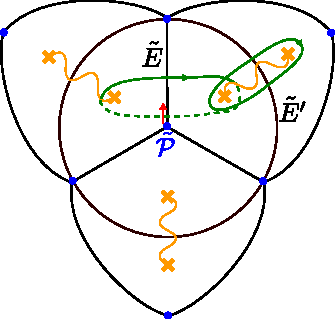
\includegraphics[width=2.5in]{figures/yin-yang-crop.pdf}
\caption{我们用来消解一个退化面的覆盖曲面。}\label{fig:yin-yang}
\end{minipage}\hspace{0.4cm}
\begin{minipage}[b]{0.45\linewidth}\centering
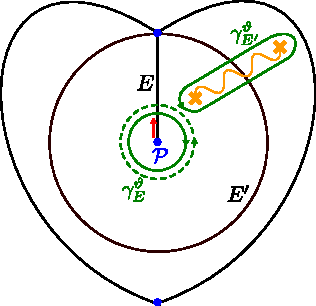
\includegraphics[width=2.25in]{figures/degenerate-loops-crop.pdf}
\caption{关联于一个退化面的闭链 $\gamma^\vartheta_{E'}$ 与 $\gamma^\vartheta_E$。}\label{fig:degenerate-loops}
\end{minipage}
\end{figure}

\subsubsection{绕奇点的圈}\label{sec:punctures}

每个奇点 $\CP_i$ 都对应着 $\Sigma$ 上一条特殊的闭链 $C_i$：它由两条小圈组成，这两条圈分处两叶、绕 $\CP_i$ 的方向相反，其定向使得：当 $E$ 是任一与 $\CP_i$ 相接的边时，有 $\langle C_i,\hat E\rangle=1$（回想提升后的边 $\hat E$ 带有自然的定向）。见图 34。% TODO 合稿改 \ref{fig:C-cycle}
\insfig{1.4in}{C-cycle}{关联于奇点 $\CP_i$ 的闭链 $C_i$。}
闭链 $C_i$ 用诸 $\gamma_E$ 表示时有简单的表达式：
\begin{equation}\label{eq:C-cycle-sum}
C_i = \sum_{E \textrm{ meeting } \CP_i} \gamma_E.
\end{equation}
这一事实对一般的顶点 $\CP_i$（即两条或更多边与之相接）如图 35 所示。% TODO 合稿改 \ref{fig:vertex-sum}
\insfig{3.7in}{vertex-sum}{对一切与顶点 $\CP_i$ 相接的 $E$ 求 $\gamma_E$ 之和，即得 $C_i$。}
若 $\CP_i$ 是退化顶点（只有一条边 $E$ 与之相接），则图 33 直接表明 $C_i=\gamma_E$。% TODO 合稿改 \ref{fig:degenerate-loops}

\subsubsection{由 $\{\gamma_E\}$ 生成的格}\label{sec:lattice-of-charges}

当 $E$ 跑遍 $T_\WKB$ 的各边时，向量组 $\{\gamma_E\}$ 生成 $\hat\Gamma$ 的一个子格；下面我们说明，它们其实生成整个格 $\hat\Gamma$。

首先说明 $\{\gamma_E\}$ 生成的格秩数正确。设 $C$ 的亏格为 $g_C$，则二次微分 $\lambda^2$ 有 $4g_C-4+2n_{\rm sing}$ 个零点。由于这些零点是单零点，由 Riemann–Hurwitz 公式，$\bar\Sigma$ 的亏格为 $g_{\bar\Sigma}=4g_C+n_{\rm sing}-3$。再用 Lefschetz 不动点公式，$H_1(\bar\Sigma;\IZ)$ 的反不变子格的秩为 $6g_C+2n_{\rm sing}-6$。把奇点也算进来，即得 $\hat\Gamma$（$H_1(\Sigma;\IZ)$ 的反不变部分）的秩为 $6g_C+3n_{\rm sing}-6$，这正好与 $\{\gamma_E\}$ 所生成的格相符。（回想方程 (5.8)。% TODO 合稿改 \eqref{eq:counts}
）于是有理向量空间 $\hat\Gamma\otimes\IQ$ 由 $\{\gamma_E\}$ 生成。由此可知，任一原始向量 $V\in\hat\Gamma$ 都可以写成 $V=\sum c_E\gamma_E$，其中 $c_E\in\IQ$。另一方面，相对同调 $H_1(\Sigma,\{\CP_i\};\IZ)$ 与 $H_1(\Sigma;\IZ)$ 互为 Poincaré 对偶，故 $\langle V,\hat E'\rangle\in\IZ$。回想 $\langle\gamma_E,\hat E'\rangle=\delta_{E,E'}$，于是可见系数 $c_E$ 实际上必须是整数。

\subsection{典范坐标的定义}

我们通过如下性质来定义 $\CX^{\vartheta,u_0}_\gamma$：对三角剖分 $T_\WKB(\vartheta,u_0)$ 中的每条边 $E$，
\begin{equation} \label{eq:canonical-darboux}
\CX^{\vartheta,u_0}_{\gamma^\vartheta_E} :=
\CX^{T_\WKB(\vartheta,u_0)}_E
\end{equation}
并且对一切 $\gamma,\gamma'$，
\begin{equation} \label{eq:CX-product}
\CX^{\vartheta,u_0}_{\gamma + \gamma'} = \CX^{\vartheta,u_0}_\gamma
\CX^{\vartheta,u_0}_{\gamma'}.
\end{equation}
由于诸 $\gamma^\vartheta_E$ 构成 $\hat\Gamma$ 的一组基，这两条性质就定义了 $\CX^\vartheta_\gamma$。

我们主要关心这些函数在固定 $u_0$ 下对 $\vartheta$ 的依赖，因此几乎总把它们记作 $\CX^\vartheta_\gamma$。

\subsection{一些简单性质}

我们先记下这些典范坐标的几条简单性质。第一，利用 (5.9)、% TODO 合稿改 \eqref{eq:fg-poisson}
\eqref{eq:intersection-pairing} 与 \eqref{eq:CX-product} 可见：用同调标号表示时，泊松结构简单地就是
\begin{equation} \label{eq:homology-poisson}
\{ \CX^\vartheta_\gamma, \CX^\vartheta_{\gamma'} \} = \inprod{\gamma, \gamma'}
\CX^\vartheta_{\gamma + \gamma'} \qquad\qquad \forall \gamma, \gamma' \in
\hat\Gamma.
\end{equation}

第二，在 (5.4) 中我们注意到：对所有与奇点 $\CP_i$ 相接的 $E$，诸 $\CX^T_E$ 之积为 $\mu_i^{2}$。% TODO 合稿改 \eqref{eq:monodromy-product}
另一方面，在第 \ref{sec:punctures} 节中我们看到：所有这些 $\gamma^\vartheta_E$ 之和就是闭链 $C_i$。把这两件事合起来，就得到一条简单规则：
\begin{equation} \label{eq:monodromy}
\CX^\vartheta_{C_i} = \mu_i^{2}.
\end{equation}

最后，我们想建立 $\CX^\vartheta_\gamma$ 所满足的实性条件。注意，由 $\CA$ 的定义 (4.8)% TODO 合稿改 \eqref{eq:def-CA}
有
\begin{equation}\label{eq:CA-conjugation}
\CA(\zeta) = - \overline{\CA(-1/\bar\zeta)}
\end{equation}
由此可知：若 $s$ 是 $\CA(\zeta)$ 的平坦截面，则 $\bar{s}/\|s\|^2$ 是 $\CA(-1/\bar\zeta)$ 的平坦截面。特别地，若 $s_i$ 是 $\CA(\zeta)$ 在某奇点 $\CP_i$ 处、角度为 $\vartheta$ 的小平坦截面，则 $\bar{s}_i/\|s_i\|^2$ 就是 $\CA(-1/\bar\zeta)$ 在 $\CP_i$ 处、角度为 $\vartheta$ 的\emph{大}平坦截面；等价地说，它是 $\CA(-1/\bar\zeta)$ 在 $\CP_i$ 处、角度为 $\vartheta+\pi$ 的小平坦截面。在 $\zeta$ 与 $-1/\bar\zeta$ 处比较定义 (5.2)，% TODO 合稿改 \eqref{eq:cross-ratio-wedges}
我们直接得到
\begin{equation} \label{eq:real-edges}
\CX^{T_\WKB(\vartheta)}_E (\zeta) = \overline{\CX^{T_\WKB(\vartheta + \pi)}_E (- 1 / \bar\zeta)}.
\end{equation}
又如通常那样有
\begin{equation} \label{eq:comp-theta}
\gamma^\vartheta_E = - \gamma^{\vartheta+\pi}_E.
\end{equation}
把 \eqref{eq:real-edges} 与 \eqref{eq:comp-theta} 结合起来，便得到所要的实性条件
\begin{equation}\label{eq:reality}
\CX^{\vartheta}_{\gamma} (\zeta) = \overline{\CX^{\vartheta+\pi}_{-\gamma} (- 1 / \bar\zeta)}.
\end{equation}

\subsection{渐近行为}\label{sec:asymptotics}

现在来到我们定义 WKB 三角剖分、并用 $H_1(\Sigma;\IZ)$ 中的闭链给坐标作标记的主要动机。我们断言：当 $\zeta\to0$ 且限制在半平面 $\IH_\vartheta$ 内时，$\CX_\gamma$ 的渐近行为简单地就是
\begin{equation} \label{eq:wkb-asymp}
\CX^\vartheta_\gamma \sim c_\gamma \exp(\zeta^{-1} \pi R Z_\gamma),
\end{equation}
其中 $c_\gamma$ 是 $\CM$ 上某个与 $\zeta$ 无关的函数。

为得到渐近式 \eqref{eq:wkb-asymp}，我们直接使用 $\CX_\gamma$ 的定义。设 $\gamma=\gamma^\vartheta_E$，其中 $E$ 是图 14 那样的一条非退化边。% TODO 合稿改 \ref{fig:quadrilateral}
这时我们将对小平坦截面（即装饰）沿各边的平行移动使用 WKB 近似。沿这些边选取一个规范，使得
\begin{equation}\label{eq:gauge-diagonal}
\varphi = \begin{pmatrix} \lambda & 0 \\ 0 & -\lambda \end{pmatrix},
\end{equation}
其中符号的选取使得 $e^{-i\vartheta}\lambda\cdot\partial_t<0$，这里 $\partial_t$ 沿 $E_{12}$、其指向为离开 $z_1$ 而朝向 $z_2$。

设 $I_1(z)$ 是 $\lambda$ 的一个原函数，定义在两条边 $E_{12}$ 与 $E_{41}$ 的一个邻域上（这里所说的「边」是一条开曲线，不含其端点）。按 WKB 近似，人们预期可以选取平坦截面 $s_1(z,\zeta)$，使得沿 $E_{12}$ 有 $\zeta\to0$ 的渐近式
\begin{equation}\label{eq:s1-asymp}
s_1(z, \zeta) \sim c_1(z) \begin{pmatrix} e^{- \frac{R}{\zeta} I_{1}(z)} \\ 0 \end{pmatrix}.
\end{equation}
附录 C% TODO 合稿改 \ref{app:wkb-error}
中我们论证情形确实如此。这一论证关键地依赖于两件事：$E_{12}$ 是一条 WKB 曲线，以及我们对 WKB 装饰的选取。要点在于：这些选取保证用 WKB 近似求 $s_1$ 时引入的误差比 $s_1$ 本身指数式地小，并且当我们沿 $E_{12}$ 演化时这一点始终保持。类似地，设 $I_2(z)$ 是 $\lambda$ 的一个原函数，定义在两条边 $E_{12}$ 与 $E_{23}$ 的一个邻域上。再次使用附录 C，可以选取 $s_2(z,\zeta)$ 使得沿 $E_{12}$ 有 $\zeta\to0$ 的渐近式
\begin{equation}\label{eq:s2-asymp}
s_2(z, \zeta) \sim c_2(z) \begin{pmatrix} 0 \\ e^{\frac{R}{\zeta} I_2(z)} \end{pmatrix}.
\end{equation}
在 $E_{12}$ 的某个一般点 $z_{12}$ 处同时计算两者，得到
\begin{equation}\label{eq:wedge-12}
s_1 \wedge s_2 \sim c_{12} \exp \left( \frac{R}{\zeta} (I_2(z_{12}) - I_1(z_{12})) \right).
\end{equation}
把指标 $1234$ 作置换，类似的论证给出
\begin{align}
s_2 \wedge s_3 &\sim c_{23} \exp \left( -\frac{R}{\zeta} (I_3(z_{23}) - I_2(z_{23})) \right), \label{eq:wedge-23}\\
s_3 \wedge s_4 &\sim c_{34} \exp \left( \frac{R}{\zeta} (I_4(z_{34}) - I_3(z_{34})) \right), \label{eq:wedge-34}\\
s_4 \wedge s_1 &\sim c_{41} \exp \left( -\frac{R}{\zeta} (I_1(z_{41}) - I_4(z_{41})) \right), \label{eq:wedge-41}
\end{align}
其中我们对记号作了显然的推广，并取 $\lambda$ 在所有边之并的一个邻域上是单值的。把这些合起来便得到
\begin{multline} \label{eq:asint}
\CX^\vartheta_\gamma \sim c_\gamma
\exp \bigg( \frac{R}{\zeta} \big(I_1(z_{41})-I_1(z_{12})+I_2(z_{12})-I_2(z_{23})+ \\  I_3(z_{23})-I_3(z_{34})+I_4(z_{34})-I_4(z_{41}) \big) \bigg).
\end{multline}
若 $\lambda$ 在整个 $Q_E$ 上是单值的，我们本可以取所有 $I_i$ 为同一个函数，那样它们就会在 \eqref{eq:asint} 中相消。由于 $Q_E$ 内部有两个分支点，这种相消并不会发生。反之，利用 $I_i(z')-I_i(z)=\int^{z'}_z\lambda$，\eqref{eq:asint} 变成
\begin{equation} \label{eq:wkb-period}
\CX^\vartheta_\gamma \sim c_\gamma \exp \left(\frac{R}{\zeta} \oint_\gamma \lambda \right).
\end{equation}
这就是关键结果：$\Sigma$ 上的周期积分是从 WKB 近似中自然浮现出来的！

若 $\gamma=\gamma^\vartheta_E$ 而 $E$ 是\emph{退化}边，我们用略微不同的方式得到同一结果。在第 \ref{sec:homology-degenerate} 节中，这个 $\gamma$ 被定义为两条小圈之和：这两条圈分别绕该顶点在覆盖上的两个提升，且方向相反。于是 $\lambda$ 的周期就由 $\varphi$ 在该顶点处的留数决定，而后者已被我们的边界条件固定：我们得到
\begin{equation} \label{eq:degenerate-period}
\oint_{\gamma} \lambda = -4 \pi i m \varepsilon(\vartheta).
\end{equation}
另一方面，由 (5.23)% TODO 合稿改 \eqref{eq:degenerate-monodromy}
我们知道 $\CX^T_E=(\mu^T)^{2}$，其中 $\mu^T$ 是绕该退化顶点的顺时针单值本征值，而它又由 (6.10)% TODO 合稿改 \eqref{eq:monodromy-formula}
给出：
\begin{equation} \label{eq:degenerate-asymptotics}
\CX^T_E \sim \exp \left[- \varepsilon(\vartheta) 4 \pi i \left( \frac{R}{\zeta} m - 2 m^{(3)} \right) \right].
\end{equation}
比较 \eqref{eq:degenerate-period} 与 \eqref{eq:degenerate-asymptotics} 可见，正如非退化边的情形一样，我们得到了预期的 \eqref{eq:wkb-period}。（这一情形下还附带一个小小的收获：给出渐近式有限部分的那个常数就是 $c_\gamma=e^{8\pi i\varepsilon(\vartheta)m^{(3)}}$。）

在证明了对一切 $\gamma^\vartheta_E$ 都成立 \eqref{eq:wkb-period} 之后，由乘性可知它对一切 $\gamma\in\hat\Gamma$ 都成立。最后回想 $Z_\gamma=\frac{1}{\pi}\oint_\gamma\lambda$，\eqref{eq:wkb-period} 就变成所要的 \eqref{eq:wkb-asymp}。

% ---------------------------------------------------------------------
% 注：原文 §7.5（From triangulations to KS symplectomorphisms）的标题始于第 5419 行，
%     不在本块范围（BRIEF 的 ch09 区间止于 5418），由 ch10 承接，此处不译标题。
% ---------------------------------------------------------------------

% =====================================================================
%  GMN2 §7.5–7.8  从三角剖分到 KS 辛同胚 / 特殊 ϑ 处的跳变 / 二次加细 / 关于全谱的评论
%  原文：wkb-paper.tex 5419–5954 行；印刷页 p.90–99
%  编号公式 (7.23)–(7.68) 共 46 条（已对照原文 PDF 逐段核过首末号）
%  脚注 2 条；插图 6 幅：图 36 flip-cycles、37 anti-cells、38/39 wkb-m±1（原文
%  \instwofigs 并排、两个 \caption，占两个图号）、40 limit-homology-annulus、
%  41 degenerate-combining-loops；另引用第 6 节的图 28（spiral-jump）
%  ch10 自 5419 行起，含 §7.5 正文（ch09 止于 5418）
%  块内公式用 \eqref；跨块引用硬编码原文编号并加 % TODO 合稿改 \ref / \eqref
% =====================================================================

\subsection{从三角剖分到 KS 辛同胚}

我们简短地盘点一下目前的进展。我们刚刚从 WKB 分析看到：坐标系 $\CX^{T_\WKB}$ 的渐近性质，可以用相应装饰三角剖分 $T_\WKB$ 的某些简单性质很好地刻画。对 $\zeta$-平面中绕原点的任意一个张角不超过 $\pi$ 的扇形 $\CV$，都可以联系一个由装饰三角剖分构成的、性状良好的子群胚 $\CT_\CV$。一个三角剖分属于 $\CT_\CV$，是指可以为其各边选取同伦代表，使之具有两条基本性质：a) 对一切 $\zeta\in\CV$，沿各边走向奇点时装饰是指数式小的；b) 沿每条边，$\lambda\cdot\partial_t$ 落在 $\CV$ 中（对 $\lambda$ 的符号作某种选取）。WKB 分析告诉我们：第 5 节% TODO 合稿改 \ref{sec:fg-coordinates}
中定义的函子，把 $\CT_\CV$ 中每个三角剖分映为扇形 $\CV$ 内具有「良好渐近」的一个达布坐标系。所谓良好渐近，指的是：每个函数都自然地用一个 $\hat\Gamma$ 中的圈来标记，并且当 $\zeta\in\CV$ 时，$\lim_{\zeta\to0}\CX_\gamma(\zeta)\exp\left[-\zeta^{-1}\pi R Z_\gamma\right]$ 有限。

由于这种标记，我们可以把每个坐标系都看作到某个抽象复环面的映射，该环面带一组傅里叶模 $\CX_\gamma$；而每个坐标变换就简单地是那个环面的一个辛同胚。对任意满足 $\vartheta_+-\vartheta_-\le\pi$ 的 $\vartheta_+,\vartheta_-$，联系坐标系 $\CX^{\vartheta_\pm}_\gamma$ 的坐标变换是一个有意思的辛同胚 $\mathbf{S}(\vartheta_+,\vartheta_-;u)$。为预先照顾到后面的结果，我们沿用第 2 节% TODO 合稿改 \ref{sec:review}
的命名。按构造，若 $\vartheta_-<\vartheta<\vartheta_+$，则 $\mathbf{S}(\vartheta_+,\vartheta_-;u)=\mathbf{S}(\vartheta_+,\vartheta;u)\,\mathbf{S}(\vartheta,\vartheta_-;u)$。

第 2 节提到的「斯托克斯因子」，出现在 $\vartheta_+$ 与 $\vartheta_-$ 分别从左、右两侧趋近同一个值 $\vartheta_0=\arg Z_{-\gamma_0}$ 的极限下。此时 $\mathbf{S}(\vartheta_+,\vartheta_-;u)\to\mathbf{S}_{\vartheta_0,u}$。显然，这些斯托克斯因子由 WKB 三角剖分 $T_\WKB(\vartheta_+)$ 与 $T_\WKB(\vartheta_-)$ 之间的比较所捕获。除非三角剖分在 $\vartheta_0=\arg Z_{-\gamma_0}$ 处跳变，否则该斯托克斯因子就是恒等变换。若三角剖分确有跳变，我们就能算出相应的辛同胚。接下来几个小节就来干这件事。

根据与第 2 节的比较，我们预期——尽管在目前阶段这远非显然——$\mathbf{S}_{\vartheta_0,u}$ 只涉及由 $\CX_{\gamma_0}$ 的函数生成的辛同胚。马上就会看到，情况确实如此：$\mathbf{S}_{\vartheta_0,u}$ 是一列 KS 因子 $\CK_{n\gamma_0}$ 的乘积，其重数正是所预期的 $\Omega(n\gamma_0)$。穿墙公式在第 2 节中被写成 $\mathbf{S}(\vartheta_+,\vartheta_-;u)$ 在 $\lambda$ 作微小改变下的不变性；于是它现在直接由装饰三角剖分 $T_\WKB(\vartheta_+,\lambda^2)$ 与 $T_\WKB(\vartheta_-,\lambda^2)$ 的不变性推出。

\subsection{特殊 $\vartheta$ 处的跳变}

\subsubsection{来自 BPS 超多重态的辛同胚}

我们已经看到，当 $\vartheta$ 越过某个对应于 BPS 超多重态的临界值 $\vartheta_c$ 时，WKB 三角剖分会跳变。现在想知道 $\CX^\vartheta_\gamma$ 在这个 $\vartheta_c$ 处如何跳变。

让我们把问题陈述得稍精确一点。当 $\vartheta$ 取在小间隔 $\vartheta_-\le\vartheta<\vartheta_c$ 内时，WKB 三角剖分的同伦类不变，记作 $T_-$。类似地，考虑小间隔 $\vartheta_c<\vartheta\le\vartheta_+$ 内的 $\vartheta$，得到三角剖分 $T_+$。我们要比较 $\CX^{\vartheta_-}_\gamma$ 与 $\CX^{\vartheta_+}_\gamma$。为减轻记号负担，下文有时把 $\vartheta_\pm$ 简写成 $\pm$。

\insfig{5.75in}{flip-cycles}{联系于三角剖分 $T_\WKB(\vartheta_\pm)$ 的诸闭链。}

图 36 画出了其中一些闭链 $\gamma^\pm_E$。% TODO 合稿改 \ref{fig:flip-cycles}
从图中可以读出它们之间的关系：
%
\begin{align}
\gamma_E^{-} &= - \gamma_E^{+}, \label{eq:flip-c1} \\
\gamma_{E_{12}}^{-} &= \gamma_{E_{12}}^{+}, \label{eq:flip-c2} \\
\gamma_{E_{41}}^{-} &= \gamma_{E_{41}}^{+} - \gamma_E^{-}. \label{eq:flip-c3}
\end{align}
%
最后两式可以简洁地概括为变换
$\gamma_{E_i}^+ = \gamma_{E_i}^- + \inprod{\gamma_{E_i}^-, \gamma_E^-}_{{}_+} \gamma_E^-$，
其中交积上的下标 $+$ 表示只取正的部分。

现在可以描述 flip 前后 $\CX_\gamma$ 之间的关系了。首先，由 (5.15)% TODO 合稿改 \eqref{eq:fg-trans-1}
看到
\begin{equation}
\CX^+_E = 1/\CX^-_E.
\end{equation}
把它与 \eqref{eq:flip-c1} 结合，并随意使用由诸 $\CX_E$ 定义 $\CX_\gamma$ 的定义式，得到
\begin{equation}
\CX^+_{\gamma_E^+} = (\CX^-_{\gamma_E^-})^{-1} = \CX^-_{\gamma_E^+}.
\end{equation}
换句话说，$\CX_{\gamma_E^+}$ 跨越射线 $\vartheta=\vartheta_c$ 时是连续的。

接下来考虑边 $E_{12}$。由 (5.16)% TODO 合稿改 \eqref{eq:fg-trans-2}
有
\begin{equation}
\CX^+_{E_{12}} = \CX^-_{E_{12}} (1 + \CX^-_E).
\end{equation}
把它与 \eqref{eq:flip-c2} 结合，得到
\begin{equation}
\CX^+_{\gamma^+_{E_{12}}} = \CX^-_{\gamma^+_{E_{12}}} (1 + \CX^-_{\gamma^-_E}).
\end{equation}
对 $\CX^\pm_{\gamma_{E_{34}}}$ 有同样的结论，只须把上式中的 $1\to3$、$2\to4$。

$E_{41}$ 的故事稍复杂些。由 (5.19)% TODO 合稿改 \eqref{eq:fg-trans-5}
有
\begin{equation}
\CX^+_{E_{41}} = \CX^-_{E_{41}} (1 + (\CX^-_E)^{-1})^{-1}.
\end{equation}
把它与 \eqref{eq:flip-c3} 结合，得到
\begin{equation}
\begin{split}
\CX^+_{\gamma^+_{E_{41}}} &= \CX^-_{\gamma^-_{E_{41}}} (1 + (\CX^-_E)^{-1})^{-1}
= \CX^-_{\gamma^+_{E_{41}}} (\CX^-_E)^{-1} (1 + (\CX^-_E)^{-1})^{-1} \\
&= \CX^-_{\gamma^+_{E_{41}}} (1 + \CX^-_E)^{-1}.
\end{split}
\end{equation}
对 $\CX^\pm_{\gamma_{E_{23}}}$ 有同样的结论，只须把上式中的 $4\to2$、$1\to3$。

为总结所得结果，我们定义
\begin{equation}
\gamma_{\rm hyper} := \gamma^-_E.
\end{equation}
这就是由那条有限 WKB 曲线所代表的 BPS 超多重态的电荷。我们得到的是
\begin{equation} \label{eq:KS-flip}
\CX^+_\gamma = \CX^-_\gamma (1 + \CX^-_{\gamma_{\rm hyper}})^{\inprod{\gamma, \gamma_{\rm hyper}}}.
\end{equation}
若取 $\Omega(\gamma_{\rm hyper})=1$——这与「该有限 WKB 曲线代表一个电荷为 $\gamma_{\rm hyper}$ 的单个 BPS 超多重态」恰好相符——并取 $\sigma(\gamma_{\rm hyper})=-1$、且对所有 $n>1$ 取 $\Omega(n\gamma_{\rm hyper})=0$，那么这正是所预期的变换性质 (2.7)。% TODO 合稿改 \eqref{eq:ks-discontinuity}

\subsubsection{来自 BPS 矢量多重态的辛同胚}

现在考虑 $\vartheta_c$ 对应于矢量多重态时会发生什么。此时，如第 6.6.3 节% TODO 合稿改 \ref{sec:vector-jump}
所讨论，$\vartheta_c$ 附近的 WKB 三角剖分含一个环带 $W$，而构成 $W$ 之三角剖分的那些边，在从任一侧令 $\vartheta\to\vartheta_c$ 时都经历一列无穷多次 flip；恰在 $\vartheta_c$ 处，我们有一个被闭合 WKB 曲线叶层化的环带。

下文将用到关于 WKB 叶层化的一些论断，它们是由计算机实验确定的。我们相信，所描述的图景至少在 $C$ 亏格为零时是正确的；不过，在本文第一个预印本版本出现之后，Ivan Smith 向我们指出：若 $C$ 的亏格 $g>0$，且环带 $W$ 截出一个含把手、不含穿刺点的连通分支，则图景可能更复杂。在 \cite{gmn5-to-appear}% TODO 待发表
中我们将给出研究该情形的另一种办法。我们将发现，即便在这种情形下，本分析的主要结果——下面的 \eqref{eq:twist-KS}——依然成立。

首先，为使图景固定下来，方便的做法是引入一些辅助对象，即把相位取为 $\vartheta+\frac{\pi}{2}$（而非 $\vartheta$）的 WKB 曲线；称它们为\emph{反 WKB 曲线}。一般而言，若有相位为 $\vartheta_c$ 的 BPS 态，就不会有相位为 $\vartheta_c+\frac{\pi}{2}$ 的 BPS 态；因此反 WKB 曲线在 $\vartheta=\vartheta_c$ 附近光滑地变化，而 WKB 曲线在该处正经历剧烈的变化。特别地，对 $\vartheta_c$ 两侧的 $\vartheta$，反分界线把含该环带的一个区域方便地划分成单连通胞腔。设 $\alpha$ 与 $\beta$ 是分属其中两个胞腔的两条反 WKB 曲线（如图 37 所示），% TODO 合稿改 \ref{fig:anti-cells}
而 $\hat\alpha$ 与 $\hat\beta$ 是它们到 $\Sigma$ 的提升（取反 WKB 定向）。利用这一划分，还可以对基准路径 $E_\pm$ 作一个典范的选取，$E_\pm$ 也画在图 37 中。
\insfig{3.3in}{anti-cells}{环带的拓扑；绿色标出的是反 WKB 曲线，另画出两条基准路径 $E_\pm$。}

如同第 5.9 节% TODO 合稿改 \ref{sec:limit-triangulation}
，我们可以把环带的种种可能三角剖分标为 $T_m$，$m\in\IZ$。当 $\vartheta$ 从上方趋于 $\vartheta_c$ 时，WKB 三角剖分依次经过一列无穷多个三角剖分；这些三角剖分可以辨认出就是 $T_m$，其中 $m=m_+,m_++1,\dots$，$m_+$ 为某个整数。类似地，当 $\vartheta$ 从下方趋于 $\vartheta_c$ 时，WKB 三角剖分依次经过另一列三角剖分 $T_m$，其中 $m=m_-,m_--1,\dots$。于是，$m$ 充分大或充分小的那些 $T_m$ 都会作为 WKB 三角剖分出现，而 $m$ 取中间值的那些 $T_m$ 则未必。为下文记号方便，我们只看 $\vartheta$ 的一个窄区间，使 $m_+>m_-$（从而每个 $T_m$ 至多出现一次）；并对每个确实出现的 $T_m$，选一个满足 $T_\WKB(\vartheta_m)=T_m$ 的 $\vartheta_m$。

当 $m>m_+$ 时，$E_{m+}$ 从奇点 $\CP'$ 出发，从一个转向点的右侧经过，向右转，绕环带顺时针缠绕并穿过 $2m$ 条反分界线，然后在到达 $\CP$ 之前从第二个转向点附近经过。$E_{m-}$ 类似，但只穿过 $2m-2$ 条反分界线。$m=1$ 的情形见图 38。% TODO 合稿改 \ref{fig:wkb-m1}
\begin{figure}[htbp]
\begin{minipage}[b]{0.5\linewidth}\centering
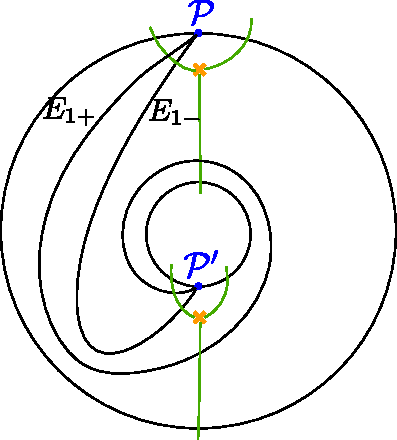
\includegraphics[width=2in]{figures/wkb-m1-crop.pdf}
\caption{$T_1=T_\WKB(\vartheta_1)$ 在环带上的拓扑。}\label{fig:wkb-m1}
\end{minipage}\hspace{0.4cm}
\begin{minipage}[b]{0.45\linewidth}\centering
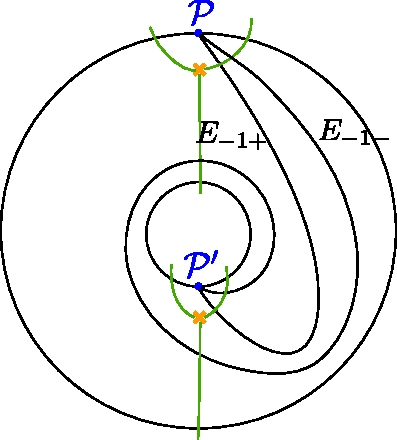
\includegraphics[width=2in]{figures/wkb-m-1-crop.pdf}
\caption{$T_{-1}=T_\WKB(\vartheta_{-1})$ 在环带上的拓扑。}\label{fig:wkb-m-1}
\end{minipage}
\end{figure}
由此可见，相应闭链满足
\begin{align}
\inprod{\gamma_{E_{m+}}^{\vartheta_m}, \hat\alpha} &= 1-m, \label{eq:int1} \\
\inprod{\gamma_{E_{m+}}^{\vartheta_m}, \hat\beta} &= 2-m, \\
\inprod{\gamma_{E_{m-}}^{\vartheta_m}, \hat\alpha} &= m, \\
\inprod{\gamma_{E_{m-}}^{\vartheta_m}, \hat\beta} &= m-1. \label{eq:int4}
\end{align}

当 $m<m_-$ 时，情况与上述非常相似，关键差别是在好几处要把「右」换成「左」。于是 $E_{m+}$ 从 $\CP'$ 出发，从一个转向点的左侧经过，向左转，绕环带逆时针缠绕并穿过 $-2m-2$ 条反分界线，然后在到达 $\CP$ 之前从第二个转向点附近经过。$E_{m-}$ 类似，但穿过 $-2m$ 条反分界线。$m=-1$ 的情形见图 39。% TODO 合稿改 \ref{fig:wkb-m-1}
此时关系 \eqref{eq:int1}–\eqref{eq:int4} 换成
\begin{align}
\inprod{\gamma_{E_{m+}}^{\vartheta_m}, \hat\alpha} &= 1+m, \label{eq:int5} \\
\inprod{\gamma_{E_{m+}}^{\vartheta_m}, \hat\beta} &= m, \\
\inprod{\gamma_{E_{m-}}^{\vartheta_m}, \hat\alpha} &= -2-m, \\
\inprod{\gamma_{E_{m-}}^{\vartheta_m}, \hat\beta} &= -1-m. \label{eq:int8}
\end{align}
现在定义四条闭链 $\gamma^\pm_{A,B}$，它们画在图 40 中。% TODO 合稿改 \ref{fig:limit-homology-annulus}
\insfig{5in}{limit-homology-annulus}{支撑在环带上方的那部分 $\hat\Gamma$ 的两组基 $\gamma^+_{A,B}$ 与 $\gamma^-_{A,B}$。}
这四条闭链满足
\begin{align}
\inprod{\gamma^+_A, \hat\alpha} = 1, \quad & \inprod{\gamma^-_A, \hat\alpha} = -1, \\
\inprod{\gamma^+_A, \hat\beta} = 1, \quad & \inprod{\gamma^-_A, \hat\beta} = -1, \\
\inprod{\gamma^+_B, \hat\alpha} = 0, \quad & \inprod{\gamma^-_B, \hat\alpha} = -2, \\
\inprod{\gamma^+_B, \hat\beta} = -1, \quad & \inprod{\gamma^-_B, \hat\beta} = -1.
\end{align}
注意由此可得
\begin{align}
\gamma^-_A &= - \gamma^+_A, \label{eq:compare-a} \\
\gamma^-_B &= - \gamma^+_B + 2 \gamma^-_A. \label{eq:compare-b}
\end{align}
另一方面，比较交积可知，这些闭链与邻近 WKB 三角剖分所附的闭链由统一公式相联系：
\begin{align}
\gamma^\pm_A & = \gamma^{\vartheta_m}_{E_{m-}} + \gamma^{\vartheta_m}_{E_{m+}}, \label{eq:gamA} \\
\gamma^\pm_B & = (1-m) \gamma^{\vartheta_m}_{E_{m-}} - m \gamma^{\vartheta_m}_{E_{m+}}, \label{eq:gamB}
\end{align}
其中左端当 $m>m_+$ 时取 $+$ 号、当 $m<m_-$ 时取 $-$ 号。

第 5.9 节中我们定义了「极限坐标系」$\CX^{T_{+\infty}}$。现在，在当前 $T_{+\infty}$ 作为 $T_\WKB(\vartheta_c)$ 出现的情形里，我们可以定义相应的同调标记：即按通常的规则 (7.3)% TODO 合稿改 \eqref{eq:canonical-darboux}
定义 $\CX^+_\gamma$，其中 $E$ 既可以指 $T_{+\infty}$ 中远离环带的一条边，也可以指特殊符号 $A$、$B$ 之一。利用 (5.32)、(5.33)、(7.48)、(7.49)，% TODO 跨块引用
可见这些坐标确实配得上「极限坐标」之名：
\begin{equation}
\lim_{\vartheta\to\vartheta_c^+} \CX^{\vartheta}_\gamma = \CX^+_\gamma. \label{eq:limit-1}
\end{equation}
类似地可以定义 $\CX^-_\gamma$；利用 (5.36)、(5.37)、(7.48)、(7.49)，% TODO 跨块引用
可见它们同样满足
\begin{equation}
\lim_{\vartheta\to\vartheta_c^-} \CX^{\vartheta}_\gamma = \CX^-_\gamma. \label{eq:limit-2}
\end{equation}

现在终于可以比较 $\CX^+_\gamma$ 与 $\CX^-_\gamma$ 了。对 $A$ 类闭链，这相当直接：利用 \eqref{eq:compare-a} 与 (5.38)% TODO 合稿改 \eqref{eq:A-relation}
可得
\begin{equation} \label{eq:twist-A}
\CX^+_{\gamma^+_A} = (\CX^-_{\gamma^-_A})^{-1} = \CX^-_{\gamma^+_A}.
\end{equation}
对 $B$ 类闭链则稍复杂些。由 \eqref{eq:compare-b} 与 (5.40)% TODO 合稿改 \eqref{eq:B-relation}
得到
\begin{equation}
\begin{split}
\CX^+_{\gamma^+_B} &= (\CX^-_{\gamma^-_B})^{-1} (\xi_+ - \xi_-)^{-4}
= \CX^-_{\gamma^+_B} (\CX^-_{\gamma^-_A})^{-2} (\xi_+ - \xi_-)^{-4} \\
&= \CX^-_{\gamma^+_B} \xi_-^{-4} (\xi_+ - \xi_-)^{-4},
\end{split}
\end{equation}
于是最终
\begin{equation} \label{eq:twist-B}
\CX^+_{\gamma^+_B} = \CX^-_{\gamma^+_B} (1 - \xi_-^2)^{-4}.
\end{equation}

定义
\begin{equation}
\gamma_{\rm vect} := - \gamma^+_A.
\end{equation}
这就是由那些闭合 WKB 曲线所代表的 BPS 矢量多重态的电荷。把结果 \eqref{eq:twist-A}、\eqref{eq:twist-B} 结合起来，得到简单的变换律
\begin{equation} \label{eq:twist-KS}
\CX^+_\gamma = \CX^-_\gamma (1 - \CX^-_{\gamma_{\rm vect}})^{-2 \inprod{\gamma, \gamma_{\rm vect}}}.
\end{equation}
注意，从图 40 可以读出 $\inprod{\gamma_B^+, \gamma_A^+}=-2$。% TODO 合稿改 \ref{fig:limit-homology-annulus}

总而言之，我们看到两个坐标系 $\CX^\pm_\gamma$ 由辛同胚 $\CK^{-2}_{\gamma_{\rm vect}}$ 相联系。于是，若取 $\Omega(\gamma_{\rm vect})=-2$——这与「闭合 WKB 曲线代表一个电荷为 $\gamma_{\rm vect}$ 的单个 BPS 矢量多重态」恰好相符——并取 $\sigma(\gamma_{\rm vect})=+1$、且对所有 $n>1$ 取 $\Omega(n\gamma_{\rm vect})=0$，我们就再次得到 $\CX_\gamma(\zeta)$ 所应满足的变换性质 (2.7)。% TODO 合稿改 \eqref{eq:ks-discontinuity}

\subsubsection{当 $m e^{-i \vartheta} \in i \IR$ 时没有辛同胚} \label{sec:no-flavor-jump}

现在处理一个棘手之处。回想每个奇点 $\CP_i$ 处都有一个参数 $m_i\in\IC$，它控制 $\varphi$ 的留数。那么，在那些使某个 $m_i e^{-i\vartheta_c}\in i\IR$ 的角度 $\vartheta=\vartheta_c$ 处，会发生什么？

如第 6.6.2 节% TODO 合稿改 \ref{sec:flavor-jump}
所述，当 $\vartheta$ 越过 $\vartheta_c$ 时，三角剖分 $T_\WKB(\vartheta)$ 在奇点 $\CP_i$ 附近跳变得相当剧烈；同时发生一次 pop，改变了平坦截面 $s_i$。另一方面，在这个 $\vartheta$ 处出现的那一族闭合 WKB 曲线并不对应带电荷的 BPS 态：它们即便是 BPS 态，也只是带味荷的态（当然，就是与穿刺点 $\CP_i$ 相关联的那个味荷）。换种说法：若按通常的办法提升这些闭合 WKB 曲线来定义 $\gamma_{\rm BPS}$，那么虽然确有 $Z(\gamma_{\rm BPS})\in e^{i\vartheta_c}\IR$，但这个电荷 $\gamma_{\rm BPS}$ 落在 $\inprod{,}$ 的根中。于是辛同胚 $\CK_{\gamma_{\rm BPS}}$ 实际上是恒等变换。因此，为与 (2.7)% TODO 合稿改 \eqref{eq:ks-discontinuity}
相容，我们应当预期：尽管 $T_\WKB$ 跳变，诸 $\CX^\vartheta_\gamma$ 在 $\vartheta=\vartheta_c$ 处\emph{不}跳变。本小节就来验证情况确实如此。

首先考虑坐标 $\CX_{C^+}$。由 (7.6)% TODO 合稿改 \eqref{eq:monodromy}
回忆到
\begin{equation}
\CX^\pm_{C^\pm} = \mu_\pm^{2}.
\end{equation}
另一方面，有
\begin{equation} \label{eq:ctrans}
C^+ = - C^-
\end{equation}
以及
\begin{equation}
\mu_+ = 1/\mu_-.
\end{equation}
于是
\begin{equation}
\CX_{C^+}^+ = (\mu_+)^{2} = (\mu_-)^{-2} = (\CX_{C^-}^-)^{-1} = \CX_{C^+}^-.
\end{equation}

\insfig{4.7in}{degenerate-combining-loops}{图 28 的一种展开；标出的是与各条边对应的同调闭链。}
还有一个 $\CX_\gamma$ 需要操心。设 $E'$ 是退化面的那条「圈」，并定义
\begin{equation}
\gamma := \gamma^{-}_{E'}.
\end{equation}
等式 $\CX^+_\gamma=\CX^-_\gamma$ 是两个不同效应相互抵消的结果。如我们在 (5.25)% TODO 合稿改 \eqref{eq:degen-loop-coord}
中所证，
\begin{equation} \label{eq:deg-1}
\CX^{\pm}_{\gamma^\pm_{E'}} = (\mu_\pm)^{-1} S,
\end{equation}
其中 $S$ 在临界迹上连续（特别地，它不涉及截面 $s$）。把图 28 展开，可以更容易看清其拓扑内容；这样得到图 41，由它可见
\begin{equation} \label{eq:degenerate-homology-jump}
\gamma^{-}_{E'} = \gamma^{+}_{E'} + C^+.
\end{equation}
把这一切合起来，即得
\begin{equation}
\begin{split}
\CX^+_{\gamma^{-}_{E'}} &= \CX^{+}_{\gamma^{+}_{E'}} \CX^{+}_{C^+} = (\mu_+)^{-1} S \mu_+^{2} \\
&= (\mu_-)^{-1} S = \CX^-_{\gamma^-_{E'}},
\end{split}
\end{equation}
正是所要的。

所以，诸 $\CX^\vartheta_\gamma$ 确实在这个 $\vartheta=\vartheta_c$ 处连续。

\subsection{二次加细} \label{sec:quadratic-refinement}

现在来看另一个烦人的细节：变换 (2.6)% TODO 合稿改 \eqref{eq:KS-Transfm}
中出现的符号 $\sigma(\gamma)$。在 \cite{Gaiotto:2008cd} 所述的一般故事中，人们预期 $\sigma:\hat\Gamma\to\IZ_2$ 是 $\hat\Gamma$ 上 mod 2 交积 $\inprod{,}$ 的一个二次加细。按定义，这意味着
\begin{equation}
\sigma(\gamma) \sigma(\gamma') = \sigma(\gamma + \gamma')\sigma(0) (-1)^{\inprod{\gamma, \gamma'}}.
\end{equation}
一般而言，人们不会指望这样的二次加细能在 $\CB$ 整体上存在；相反，必须在不同的局部补片上选取不同的加细，而在把补片粘合起来时，还必须追踪诸 $\CX^\vartheta_\gamma$ 中某些符号的变化，其来源正是这些加细彼此不同。

另一方面，在本文中我们似乎发现了一个更简单的故事。诸函数 $\CX^\vartheta_\gamma$ 的粘合律不涉及任何刁钻的符号。此外，只要取
\begin{align} \label{eq:dessigma}
\sigma(\gamma_{\rm hyper}) &= -1, \\
\sigma(\gamma_{\rm vect}) &= +1, \label{eq:dessigma2}
\end{align}
我们为诸 $\CX^\vartheta_\gamma$ 找到的变换就与 (2.6)% TODO 合稿改 \eqref{eq:KS-Transfm}
相符。这怎么能相容呢？只要存在\emph{一个}二次加细 $\sigma$，对所有在某个 $u\in\CB$ 的谱中出现的超多重态与矢量多重态都满足 \eqref{eq:dessigma}、\eqref{eq:dessigma2}，那就相容了。

对任意固定的 $(\vartheta,u)$，我们很容易构造这样的 $\sigma$：只须要求 $\sigma(0)=+1$、对 $T_\WKB(\vartheta,u)$ 的一切非退化边 $E$ 都有 $\sigma(\gamma_E)=-1$、而对退化边有 $\sigma(\gamma_E)=+1$，它就被确定了。由这个定义不难看出：对一切相位为 $\vartheta$ 的 BPS 态，都有 $\sigma(\gamma_{\rm hyper})=-1$、$\sigma(\gamma_{\rm vect})=+1$。于是从这个角度看，麻烦在于要证明如此定义的 $\sigma$ 其实与 $(\vartheta,u)$ 无关。这归结为验证：当三角剖分 $T_\WKB$ 跳变时，上述 $\sigma$ 的公式与诸 $\gamma_E$ 的变换相容。幸运的是，情况确实如此。

的确，如我们已讨论过的，随着 $(\vartheta,u)$ 变化，WKB 三角剖分经历三类变换。第一类（超多重态）由 \eqref{eq:flip-c1}–\eqref{eq:flip-c3} 给出，直接验证可知它与我们对 $\sigma$ 的提法相容。第二类（矢量多重态）用 \eqref{eq:gamA}、\eqref{eq:gamB} 所定义的辅助闭链 $\gamma_{A,B}$ 来表述；利用这两式以及我们对 $\sigma$ 的提法，可得 $\sigma(\gamma_A)=+1$、$\sigma(\gamma_B)=-1$。这个 $\sigma$ 确实与变换 \eqref{eq:compare-a}、\eqref{eq:compare-b} 相容。最后，第三类跳变（$m/e^{i\vartheta}\in i\IR$）中闭链的变换由 \eqref{eq:ctrans} 与 \eqref{eq:degenerate-homology-jump} 给出，它同样与 $\sigma$ 相容（回想 $C_+$ 对应一条退化边，故 $\sigma(C_+)=+1$）。

描述这个二次加细，还有一种更内蕴的办法。给定任一闭链类 $\gamma\in H_1(\Sigma;\IZ)$，先把 $\gamma$ 表示成一族互不相交的、避开 $\lambda$ 之零点的定向闭曲线之并。在每条闭曲线上都有\emph{相位函数}，定义为 $\lambda\cdot\partial_t$ 的相位。令 $n_w$ 表示沿该曲线绕行一周时此相位绕圆周转过的圈数，则 $\sigma(\gamma)$ 就是 $(-1)^{n_w+1}$ 对我们为 $\gamma$ 所选代表的所有分支求积。不难验证：这确实作为同调上的函数良定义，并且给出一个二次加细。此外，由「$\gamma_{\rm hyper}$ 可由单条闭合的常相位曲线代表，而 $\gamma_{\rm vect}$ 可由两条这样的曲线之并代表」这一事实，容易看出 $\sigma$ 具有所要的性质 \eqref{eq:dessigma}、\eqref{eq:dessigma2}。

\subsection{关于全 BPS 谱的评论} \label{sec:bps-comments}

至此，在与带正则奇性的 $SU(2)$ Hitchin 系统相关的那一类例子里，我们已经构造出函数 $\CX^\vartheta_\gamma$，并验证了它们在 $\vartheta$ 变化时按 KS 变换跳变。如我们在上面以及第 2 节中所解释的，这些函数是我们解释穿墙公式的关键要素。但这还不是全部：我们还学到了一种确定 BPS 谱的策略。的确，若取两个相位 $\vartheta_\pm$ 并算出 WKB 三角剖分 $T_\WKB(\vartheta_\pm,u)$，就能重构坐标变换 $\mathbf{S}(\vartheta_+,\vartheta_-;u)$，按第 2.3 节% TODO 合稿改 \ref{subsec:wallcrossing}
所述把它唯一地分解成适当排序的 KS 变换之积，并读出相位落在扇形 $[\vartheta_-,\vartheta_+]$ 内的 BPS 态谱。

若取 $\vartheta_+=\vartheta_-+\pi$，这个策略就格外有力。\footnote{确切地说，我们只把两条边界射线中的一条算进该扇形。} 此时扇形是整个半平面，因而大到足以确定整个 BPS 谱（相位在此半平面之外的 BPS 态，正是在其中的那些态的反粒子）。因此我们把 $\mathbf{S}(\vartheta,\vartheta+\pi;u)$ 称为「谱生成元」。幸运的是，与任意的 $\mathbf{S}(\vartheta_+,\vartheta_-;u)$ 不同，这个谱生成元其实是可计算的！可计算性的根本原因在于：$T_\WKB(\vartheta)$ 与 $T_\WKB(\vartheta+\pi)$ 只在装饰上不同——要从前者变到后者，只须在全部奇点处作 pop。谱生成元的计算推迟到第 11 节% TODO 合稿改 \ref{sec:UniversalStokesMatrix}
，但现在可以指出：结果相当简单，并且只依赖于 $T_\WKB(\vartheta,u)$ 的组合数据。

若能\emph{从物理上}理解 $T_\WKB(\vartheta,u)$ 为何能捕获整个 BPS 谱，将会非常有意思。这个故事的至少一部分容易理解：对 $T_\WKB(\vartheta,u)$ 的每条边 $E$，真空 $u$ 中都存在一个电荷为 $\gamma_E$ 的 BPS 超多重态。的确，WKB 叶层化中相应的胞腔被坐标变换 $z\mapsto w=\int^z\lambda$ 映成一条带，两个转向点位于该带的两条相对边界上；而 $w$-平面中连接这两个转向点的一条直线段在 $z$-平面中的原像，就给出电荷为 $\gamma_E$ 的一条 BPS 弦。\footnote{对极限三角剖分有类似的陈述：此时每个被 WKB 曲线叶层化的环带给出一族闭合 BPS 弦（一个矢量多重态），外加一座无穷高的超多重态之塔，它们就是 $w$ 坐标中转向点之间各条直线路径的原像，带有绕环带的各种缠绕。}

这些 BPS 粒子的电荷 $\gamma_E$ 构成电荷格的一组基，如第 7.1.4 节% TODO 合稿改 \ref{sec:lattice-of-charges}
所证。其实还有更多：这组基具有一条重要的正性性质，令人想起单李代数中根与单根的关系。回想一个 BPS 态对应一条有限 WKB 曲线，它在 $w$-平面中给出一个直线段；该线段的斜率就是此 BPS 态中心荷的相位。特别地，若这个相位落在 $\vartheta$ 与 $\vartheta+\pi$ 之间，则该 BPS 弦与相位为 $\vartheta$ 的 WKB 曲线有\emph{正}交积。另一方面，按第 7.1 节% TODO 合稿改 \ref{sec:homology}
所给同调标记的定义，$\inprod{\gamma_E^\vartheta, \hat E'}=\delta_{E,E'}$。于是，若某同调闭链 $\gamma_{\rm BPS}$ 承载一个相位介于 $\vartheta$ 与 $\vartheta+\pi$ 之间的 BPS 态，就有
\begin{equation}
\gamma_{\rm BPS} = \sum_E c_E \gamma_E^{\vartheta}
\end{equation}
且一切 $c_E\ge0$。

上述事实引出一些自然的猜测。首先，这种正分解暗示：所有 BPS 态都可以看作一组「简单」BPS 态的束缚态，而这些简单态与 $T_\WKB(\vartheta,u)$ 的各条边 $E$ 一一对应。这个猜想还有进一步的证据：谱生成元 $\mathbf{S}$ 可以纯粹由 $T_\WKB$ 的组合数据算出。

注意，即便真空 $u$ 固定，改变 $\vartheta$ 也能得到简单 BPS 态的各种不同的基。这令人想起用箭图量子力学描述 BPS 态的常见做法：在那个故事里，人们有时用各种不同的箭图描述同一个量子力学，这些箭图对应不同的「例外集」（exceptional collections），彼此由变异相联系。的确，在我们的语境中，天然地就有一个箭图：其节点用三角剖分的边 $E_i$ 标记，箭头的数目由 $\inprod{E_i,E_j}$ 决定。有可能：取适当的 FI 项与超势之后，该箭图量子力学的 BPS 态会与理论中相位落在扇形 $[\theta,\theta+\pi]$ 内的全部 BPS 谱一一对应。箭图的变异与「簇变换」之间的关系——后者与我们在本文中遇到的 KS 变换密切相关——已在数学文献中被广泛研究（例如见 \cite{cluster-intro}）。（这一方向的进一步发展，见例如 \cite{Gaiotto:2010be,Cecotti:2010fi,Cecotti:2011rv}。）

% =====================================================================
%  GMN2 §8 不规则奇点 + §9.1–9.3 线性 SU(2) 箭图的标度极限
%  原文：wkb-paper.tex 5955–6356 行；印刷页 p.100–106（PDF p.101–107）
%  编号公式 (8.1)–(8.5)、(9.1)–(9.15) 共 20 条；插图 2 幅（图 42、图 43）
%  备注：原文 §9.3 末尾的 align 在 PDF 上占两个编号 (9.14)(9.15)，
%        故本块编号式为 5 + 15 = 20 条（BRIEF 表估 18 条，实测 20 条）。
%        跨块引用一律硬编码原文编号并加 % TODO；块内引用用 \eqref。
% =====================================================================

\section{不规则奇点}\label{sec:irregular}

过去三节我们一直关注正则奇点的情形，但这些构造也可以搬到不规则奇点的情形。故事与正则情形颇为相似，只需作如下修改：

\begin{enumerate}

\item 我们首先给出包含不规则奇点时的三角剖分的适当概念。设 $\CP_*$ 是一个不规则奇点，$\lambda^2$ 在那里有 $L+2$ 阶极点，其中 $L \geq 1$ 为整数。（第 3 节% TODO 合稿改 \ref{sec:physics}
对秩为二的 Hitchin 系统给出的边界条件涉及 $L = 1$ 的不规则奇点；而在第 9 节% TODO 合稿改 \ref{section:Superconformal}
中我们会遇到 $L = N+2$、$N\geq 0$ 的奇点。）我们在 $\CP_*$ 周围画一个圆 $S^1(\CP_*)$，它围出一个圆盘 $D(\CP_*)$，视之为无穷小。在这个圆上标出 $L$ 个点 $Q_i$，$i=1, \dots, L$。这些点的循环次序规定为：$\dots, Q_i, Q_{i+1}, \dots$ 绕 $\CP_*$ 顺时针排列。于是我们的三角剖分其实是曲面 $C'$ 的三角剖分，而 $C'$ 由把所有圆盘 $D(\CP_*)$ 挖掉得到。顶点是所有不规则奇点周围的标号点 $Q_i$，再加上全部正则奇点 $\CP_i$。边必须包含圆周 $S^1(\CP_*)$ 上连接相邻点 $Q_i$ 的那些弧段。我们把这些弧段称为\emph{边界边}；它们在下面会有特殊地位。

\item 为了定义一个\emph{装饰}三角剖分，我们需要在每个顶点附近为联络 $\CA$ 选一个平坦截面（只定到标度因子）。对不规则奇点，这意味着在 $S^1(\CP_*)$ 上的每个点 $Q_i$ 附近各选一个平坦截面。与正则情形一样，我们希望把这一选择缩小为离散的选取。为此我们注意到：在不规则奇点的情形，除可能存在的单值之外，还有斯托克斯现象。\footnote{以下我们假定：复曲线上\emph{亚纯}联络的标准斯托克斯理论可以按最明显的方式推广，以适用于联络 $\CA$——它平坦，但并不亚纯。关于这一确切情形，我们没有找到任何文献，不过 \cite{MR1864833} 中有一些多少相关的构造。}从 $\CP_*$ 发出 $L$ 条射线（「斯托克斯射线」），围出张角为 $2\pi/L$ 的扇区。一个平坦截面若沿着斯托克斯射线某一侧的、指向 $\CP_*$ 的射线当 $z \to \CP_*$ 时渐近地指数式小，那么它在斯托克斯射线的另一侧就变成指数式大。\footnote{在关于斯托克斯现象的文献中有两类射线，分别称为 \emph{Stokes} 与 \emph{anti-Stokes}，二者在理论的系统展开中都起重要作用。遗憾的是，这一术语在各家作者的用法中并不一致。按我们的约定，标准 Airy 函数 $Ai(x)$ 沿正实轴有实的指数衰减，沿负实轴则有多项式型衰减并带振荡包络；它的斯托克斯射线位于负实轴以及 $\vert {\rm arg}(x)\vert = \pi/3$ 处。}我们这样定义一个装饰：取 $Q_i$ 附近的一个平坦截面（模去整体重标度），使得绕 $\CP_*$ 作解析延拓之后，它当 $z \to \CP_*$ 时在由斯托克斯射线围成的\emph{某个}扇区内指数式小。

\item 这样的截面（模去重标度）可以排成一个无穷序列
\begin{equation}\label{eq:bisequenceStokes}
\cdots, s_{-3}, s_{-2}, s_{-1}, s_0, s_1, s_2, s_3, \dots
\end{equation}
其排序规定为：若 $s_n$ 是扇区 $\CS$ 中的小解，则 $s_{n+1}$ 就是沿顺时针方向的下一个扇区中的小解。（若单值平凡，则可选取 $s_n$ 的标度，使该序列以 $L$ 为周期。）此外我们进一步限制装饰的选取：若在点 $Q_i$ 处选了 $s_n$，那么在点 $Q_{i+1}$ 处也必须选 $s_{n+1}$，如此递推。于是，不规则奇点处装饰的选取归结为在\emph{一个}标号点上选一个平坦截面，而不是在每个点上独立地选。因此，不规则奇点附近一切可能的装饰构成一个 $\IZ$-挠子；若单值平凡，它可以化归为 $\IZ_L$-挠子。

\item Fock–Goncharov 坐标 $\CX_E^T$ 的定义现在可以照旧给出，只需注意一条重要约定：若 $E$ 是边界边，则规定 $\CX_E^T = 0$。

\item 不规则奇点附近 WKB 叶状结构的局部行为，与正则奇点附近相当不同。每条 WKB 曲线不再各向同性地盘旋进入奇点，而是渐近地切于 $L$ 条射线之一。这些射线（相位为 $\vartheta$）我们称为 \emph{WKB 射线}，它们在不规则奇点 $\CP_*$ 周围的无穷小圆 $S^1(\CP_*)$ 上决定 $L$ 个点 $Q_i$，$i=1, \dots, L$；这些正是我们定义 $T_\WKB$ 时要用的标号点。若 $\vartheta = \arg \zeta$，则相位为 $\vartheta$ 的 WKB 射线与联络 $\CA$ 的反斯托克斯射线重合。
\insfig{2.7in}{petals}{$L = 4$ 的不规则奇点附近 WKB 叶状结构的局部行为。WKB 曲线聚集到这 $4$ 条 WKB 射线上，相邻射线之间相隔 $\pi/2$ 弧度的弧段。在奇点的小邻域内，WKB 曲线形如花瓣，把相邻的 WKB 射线连接起来。}

\item $T_\WKB$ 的定义本质上与之前一样。若一条 WKB 曲线渐近地趋向某条终止于不规则奇点 $\CP_*$ 的 WKB 射线，我们就认为它终止于 $S^1(\CP_*)$ 上相应的点 $Q_i$。于是照常，分界 WKB 曲线把 $C'$ 切成若干胞腔，每个胞腔由一般的 WKB 曲线叶状铺满，而 $T_\WKB$ 的边由每个胞腔中取一条一般 WKB 曲线构成。注意有些一般 WKB 曲线完全落在不规则奇点的任意小邻域内，并把相邻的 WKB 射线连接起来，如图 42 所示% TODO 合稿改 \ref{fig:petals}
。$T_\WKB$ 的边中有 $L$ 条这样的曲线，它们就是上面提到的、连接相邻 $Q_i$ 的边界边。每条这样的边围出一个触及 $\CP_*$ 的花瓣状区域；圆盘 $D(\CP_*)$ 就是这 $L$ 个花瓣的并。

\item $T_\WKB$ 在顶点 $Q_j$ 处的装饰，取这样的平坦截面：沿穿过 $Q_j$、指向 $\CP_*$ 的 WKB 射线走时，它变得指数式小。让我们把这个截面描述得更精确些。把 $\CP_*$ 放在 $z = \infty$，并设那里 $\lambda^2 \sim z^{L-2} dz^2$。$L$ 条 WKB 射线位于
\begin{equation}\label{eq:PolyRays}
r_j := \left\{ \arg(z) = \frac{2}{L} \vartheta + \frac{2\pi j}{L} \right\}, \quad j=1, \dots, L.
\end{equation}
当 $z \to \infty$ 时，平坦截面的形式渐近式形如
\begin{equation}\label{eq:ch11-formal-asymp}
\exp \left[ \pm \frac{2}{L}\frac{R}{\zeta} z^{\half L} + \cdots \right] s_{const}.
\end{equation}
特别地，其范数由指数实部的符号控制，而该符号在斯托克斯射线
\begin{equation}\label{eq:ch11-stokes-rays}
{\rm arg}(z) = \frac{2}{L}\vartheta_\zeta + \frac{(2j+1)\pi}{L}, \qquad j = 0, \dots, L-1
\end{equation}
两侧发生改变，其中我们记 $\vartheta_\zeta = \arg \zeta$。只要 $e^{i\vartheta} \not= - e^{i\vartheta_\zeta}$，由这些斯托克斯射线围成的每个扇区中都恰含一条 WKB 射线 $r_j$。沿这条 WKB 射线，一般平坦截面的范数渐近于
\begin{equation} \label{eq:norm-sign}
\exp\left[ \pm \frac{ 2 R}{L} \frac{\vert z\vert^{L/2}}{\vert \zeta\vert} \Re \left(e^{i (\vartheta + \pi j - \vartheta_\zeta)} \right) + \cdots \right].
\end{equation}
若在 \eqref{eq:norm-sign} 中取的 $\pm$ 号与 $\Re\left(e^{i (\vartheta + \pi j - \vartheta_\zeta)} \right)$ 的符号相反，则对任何 $\zeta \in \IH_\vartheta$，该范数沿 $r_j$ 当 $z \to \infty$ 时指数式小。到此为止我们只讨论了形式渐近；但有一条重要的原理：存在唯一的平坦截面（称为「小截面」），它的范数沿 $r_j$ 确实具有这种指数式小的渐近行为（对 $\zeta \in \IH_\vartheta$）。我们就选这个小截面作为 $T_\WKB(\vartheta)$ 在 WKB 射线 $r_j$ 处的装饰。它由 $\vartheta$ 与 $j$ 典范地确定。微妙之处在于：当 $\zeta$ 绕 $0$ 一圈时，这个小截面一般带有非平凡的单值；由此可见，它实际依赖于 $\vartheta \in \IR$，而不只是 $\vartheta \in \IR / 2 \pi \IZ$。

\item $\gamma^\vartheta_E$ 与 $\CX^\vartheta_{\gamma}$ 的定义与只有正则奇点的情形完全相同。当 $E$ 是边界边时，我们不定义这个圈。

\item 我们把不规则奇点 $\CP_*$ 处的 pop 定义为该处装饰的 $\IZ$-挠子上按 $1$ 的作用。为确定约定：若 $\dots, Q_j, Q_{j+1}, \dots$ 按顺时针排列，而装饰给它们配上截面 $\dots, s_n, s_{n+1}, \dots$，则 pop 之后配上的是 $\dots, s_{n-1}, s_{n}, \dots$。若把 $\vartheta$ 换成 $\vartheta + \pi$，则 $T_\WKB(\vartheta)$ 在每个不规则奇点处的装饰都经历一次 pop。

\item 可能出现这样的情况：一串 flip 产生的新三角剖分，与原来的只差某个边界圆旋转 $2\pi/L$，等价地说，只差 $Q_i$ 的一个循环置换。这与在不规则顶点处作一次 pop 的效果完全相同。这反映了装饰三角剖分之群胚中态射之间的一个关系。

\end{enumerate}

\section{线性 $SU(2)$ 箭图的标度极限：单个不规则奇点的情形}\label{section:Superconformal}

% TODO 图注中「第 9 节」为硬编码（原文 \protect\ref{section:Superconformal}），合稿时核对
\insfig{3.5in}{quiver-of-twos}{第 9 节所考虑理论的线性箭图。}

本节用一些格外简单的理论来说明第 5–8 节% TODO 合稿改 \ref{sec:fg-coordinates}–\ref{sec:irregular}
的某些考虑。这些理论是 $n$ 个 $SU(2)$ 规范群的线性箭图的某些标度极限，其中首、末两个规范群各带两个基本超多重态，如图 43 所示% TODO 合稿改 \ref{fig:quiver-of-twos}
。相应的 Hitchin 系统规范群为 $SU(2)$，并且在标度极限之后，在 $C = \IC\IP^1$ 上只有一个奇点，而且是不规则奇点。

\subsection{线性 $SU(2)$ 箭图及其参数空间}

这个理论有 $3n+3$ 个物理参数：紫外拉氏量中含 $n$ 个规范耦合、$n-1$ 个双基本表示质量与 $4$ 个基本表示质量；而库仑分支由 $n$ 个真空期望值 $\langle {\Tr}(\Phi^{(\alpha)})^2 \rangle$ 参数化。

回忆第 3 节% TODO 合稿改 \ref{sec:physics}
：相应的 Seiberg–Witten 曲线是 $F(t, v) = 0$，其中
\begin{equation}\label{eq:ch11-Ftv}
F(t,v) = \sum_{\alpha=0}^{n+1} q_\alpha (v) t^{n+1-\alpha} = p_0(t) v^2 + p_1(t) v + p_2(t).
\end{equation}
此外我们已经看到，可以（带有某些冗余地）参数化为
\begin{equation}\label{eq:ch11-qalpha}
q_\alpha(v) = c_\alpha (v^2 - \mu_\alpha v - u_\alpha).
\end{equation}
在弱耦合区域，耦合由 $c_\alpha$ 确定，质量由 $\mu_\alpha$ 与 $u_\alpha$ 确定，而库仑分支由 $u_\alpha$ 参数化。最后，正如我们在 (3.77) 处看到的% TODO 跨块引用
，把质心自由度分离出去之后，Seiberg–Witten 曲线就成为某个 $SU(2)$ Hitchin 系统的谱曲线，其中
\begin{equation}\label{eq:ch11-lambda2}
\lambda^2 = \half \frac{p_1(t)^2 - 4 p_2(t) p_0(t) }{(t p_0(t))^2} dt^2.
\end{equation}
这个二次微分在 $t = 0$ 与 $t = \infty$ 处有二阶极点，在 $p_0(t)$ 的 $n+1$ 个零点处也有二阶极点。

以上描述多少掩盖了问题的 S-对偶性质 \cite{Witten:1997sc,Gaiotto:2009we}。物理规范耦合其实只依赖于带 $n+3$ 个标号点的球面之模空间中的一个点。而且，双基本表示质量参数与基本表示质量参数之间并没有 S-对偶不变的区别。这些事实提示：我们应当更一视同仁地对待这 $n+3$ 个奇点与质量参数。办法是在描述中引入一些冗余，即从 $[t:1] \in \IC\IP^1$ 到新坐标 $z$ 作一般的分式线性变换。作这样的变换之后我们得到（多项式下标表示其次数）
\begin{equation}\label{eq:quad-diff-1}
\lambda^2 = \frac{Q_{2n+2}(z)}{(D_{n+3}(z))^2} (dz)^2.
\end{equation}
扣掉 $SL(2,\IC)$ 作用的 $3$ 个参数与 $Q$、$D$ 同时重标度的 $1$ 个参数之后，仍有 $3n + 7 - 4 = 3n+3$ 个物理参数。

如已提到，这些物理参数的地位并不平等。耦合与质量指定紫外理论，而库仑分支参数指定真空。为凸显这一区别，把 $\lambda^2$ 稍作不同的参数化是有用的。

$n+3$ 个质量参数可以刻画为 $\lambda^2$ 中 $n+3$ 个极点的留数。（我们不考虑其中某些极点相撞的情形——那对应物理理论的强耦合奇点。）若这些极点位于 $z_a$，$a = 1, \dots, n+3$，并假定所有 $z_a \neq \infty$，则可以把 $\lambda^2$ 写成如下形式：
\begin{equation}\label{eq:part-frac}
\lambda^2 = \sum_{a=1}^{n+3} \left(
\frac{m_a^2}{(z-z_a)^2} + \frac{c_a}{z-z_a}\right) dz^{2}.
\end{equation}
要求 $\lambda^2$ 在 $z = \infty$ 处正则，给出对 $c_a$ 的三个条件：
\begin{equation}\label{eq:c-conds}
\begin{aligned}
\sum_{a=1}^{n+3} c_a & = 0, \\
\sum_{a=1}^{n+3} z_a c_a & =   - \sum_{a=1}^{n+3} m_a^2, \\
\sum_{a=1}^{n+3} z_a^2 c_a & =   - 2\sum_{a=1}^{n+3} m_a^2 z_a.
\end{aligned}
\end{equation}
库仑分支 $\CB$ 就是满足 \eqref{eq:c-conds} 的 $c_a$ 构成的空间。由于 \eqref{eq:c-conds} 是关于 $c_a$ 的非齐次线性方程，它是一个 $n$ 维仿射空间。

（另一种看法是：一旦通过 $z_a$ 指定了耦合，带任意质量与真空的理论空间就是一个线性空间——多项式 $Q_{2n+2}(z)$ 的空间——它也可以看作 $H^0(\IC \IP^1, K^{\otimes 2} \otimes \CO(2\CP_1 + \cdots + 2\CP_{n+3}) )$。固定质量于是固定这个空间的一个仿射子空间。）

\subsection{标度极限}

对一般的质量，库仑分支的奇点出现在 $Q_{2n+2}(z)$ 的两个或多个根重合之时。在这些点上库仑分支的度量奇异，绕该轨迹的涨落具有无穷大的作用量。原因当然是：在这个轨迹上至少有一个 BPS 态变成无质量。$Q_{2n+2}(z)$ 的零点落在判别式轨迹 $\CD$ 上，$\CD$ 带有分层 $\CD_k$，其中恰有 $k$ 个零点重合。下面我们集中看一个分层 $\CD_N$。在该轨迹附近，若干个 BPS 态变轻，我们想关注这些态的低能物理。

相应地，我们考虑如下的标度极限。取一点 $\CP \in C$ 及局部坐标 $z$，使 $z(\CP) = 0$。$Q$ 的空间中的有关邻域可以用 $Q_{2n+2}(z) = \prod_{i=1}^N (z - \epsilon \theta_i) \tilde Q_{2n+2-N}(z)$ 参数化，其中 $\tilde Q_{2n+2-N}(0) \not= 0$。当 $\epsilon \to 0$ 时，$Q$ 的 $N$ 个零点在 $z = 0$ 处相撞。与连接其中两个相撞零点的弦相应的典型 BPS 态，其质量为 $\epsilon^{(N+2)/2}$ 阶。于是我们考虑这一能标及以下的物理。我们还用 $z = \epsilon \tilde z$ 定义黎曼面 $C$（即 M5-膜世界体）上的一个标度区域；我们只考虑定域在这个区域内的涨落。对 Seiberg–Witten 微分 $\lambda$ 与 $\tilde z$ 作适当重标度之后，我们于是考虑一个理论，其中
\begin{equation}\label{eq:PolyDegen}
\lambda^2 = P_N(z) dz^2,
\end{equation}
$P_N$ 是 $N$ 次首一多项式，而我们这片 M5-膜世界体上的标度区块已被放大成整个复平面。

原理论的许多形变在标度极限下变得不可归一化；不过有些形变仍然可归一化。它们就是多项式形变 $P_N \to P_N + \delta P_N$，满足
\begin{equation}\label{eq:ch11-normaliz}
\int_{\IC} \vert \delta \lambda \vert^2 = \int_{\IC} \biggl\vert
\frac{\delta P_N(z) }{2 \sqrt{P_N(z)}} \biggr\vert^2 d^2 z < \infty.
\end{equation}
由于 $P_N(z)$ 的零点是单零点，发散只可能来自 $z \to \infty$，因此可归一化条件为
\begin{equation}\label{eq:ch11-deltaP}
\delta P_N = \sum_{i < \half(N-2)} \delta p_i z^i.
\end{equation}

对这个可归一化条件还有另一种有用的看法，即固定 $\sqrt{P_N(z)}$ 在 $z = \infty$ 附近展开的奇异部分：
\begin{equation}\label{eq:AsympOfP}
\sqrt{P_N(z)} = \Delta(z) + o(z^{-1})
\end{equation}
其中 $\Delta(z)$ 固定（由我们多半已经丢弃的紫外理论决定）。

$N$ 为偶与 $N$ 为奇之间有一个重要差别。当 $N$ 为偶时，$\Delta(z)$ 是整数幂的展开，以一个单极点收尾；我们把它的留数记作 $m$。变动 $m$ 是「对数可归一化」形变，对应 $i = \half(N-2)$。稍后我们从 Hitchin 系统过渡到平坦联络时就会看到，$m$ 指定了 $\infty$ 处的形式单值。当 $N$ 为奇数时，不存在这样的对数可归一化形变。

标度极限之后，库仑分支上仍然存在奇点轨迹，使某些 $\theta_i = \theta_j$，即 $P_N(z)$ 有多重零点。这些轨迹是 $\CD$ 的高维分层与 $\CD_N$ 周围标度区域的交。在这些轨迹上某些 BPS 态变成无质量。而且，在有些情形下变成无质量的 BPS 态彼此非定域，从而导致 \cite{Argyres:1995jj,Argyres:1995xn} 中所研究的那类理论。

要到达最极端的情形，我们可以调节不可归一化参数，使得所考虑的是 $\lambda^2 = z^N (dz)^2$ 的可归一化形变。模空间中这一点的深红外物理由一个超共形场论描述 \cite{Argyres:1995jj,Argyres:1995xn}；并且可以用上面找出的可归一化形变对此理论作微扰，从而定义一个具有有限 BPS 谱的紫外完备量子场论。于是我们研究的就是这些理论的 Seiberg–Witten 曲线与 BPS 态。从由线性箭图指定的原紫外理论的观点看，我们关注的是模空间某个区域内的一个低能子部门，在那里若干 BPS 态正变得参数式地轻。如下文将看到的，这类态的数目被 $\half N(N-1)$ 界住 \cite{Shapere:1999xr}。

\subsection{Hitchin 系统}\label{subsec:HitchinForAD}

上一小节我们描述了 Hitchin 系统谱曲线的一种退化。为使讨论完整，现在说明 Hitchin 系统相应的退化。新的 Hitchin 系统定义在 $\IC\IP^1$ 上，在 $z=\infty$ 处只有一个不规则奇点。具体地说，当 $N$ 为偶时我们有
\begin{equation}\label{eq:ch11-A0}
A_0 = \begin{pmatrix} -m^{(3)} & 0 \\ 0 & m^{(3)}
\end{pmatrix} \left( \frac{dz}{z} - \frac{d \bar z}{\bar z} \right)
\end{equation}
以及
\begin{equation}\label{eq:ch11-varphi0}
\varphi_0 = \begin{pmatrix} \Delta(z) & 0 \\  0 & - \Delta(z)
\end{pmatrix},
\end{equation}
其中 $\Delta(z)$ 如 \eqref{eq:AsympOfP} 所定义。由于 $\Delta(z) \sim z^{N/2} + \cdots + \frac{m}{z}$，逆时针绕行下的形式单值为
\begin{equation}\label{eq:MonodromyAtInfinity}
\exp \left(2\pi i \left[ \frac{mR}{\zeta} - 2 m^{(3)} - \bar m R
\zeta \right]\sigma^3 \right).
\end{equation}
其特征值我们记作 $\mu^{\pm 1}$。

当 $N$ 为奇数时，没有与质量参数 $m, m^{(3)}, \bar m$ 类似的东西。取而代之，我们有 (3.115) 的一个推广% TODO 跨块引用
：
\begin{align}\label{eq:NoddBC}
\varphi_0 & = \Delta(z) \begin{pmatrix} 0 & (\bar z/z)^{1/4} \\
(z/\bar z)^{1/4} & 0 \end{pmatrix}, \\
A_0 & = \frac{1}{8} \sigma^3
\left(\frac{dz}{z} - \frac{d\bar z}{\bar z}\right).
\end{align}

\begin{yizhu}
$\IZ$-挠子（$\IZ$-torsor）指以 $\IZ$ 为结构群的主齐性空间：它本身没有自然的原点，但任意两个元素之差是一个整数。装饰的选取构成 $\IZ$-挠子，意味着「选定一个装饰」与「选定一个整数偏移」是等价的。
\end{yizhu}

% =====================================================================
%  GMN2 §9.4  例子：N = 1, 2, 3
%  原文：wkb-paper.tex 6357–6845 行；印刷页 p.107–115；编号公式 (9.16)–(9.35) 共 20 条；无脚注
%  图：44 N2plot / 45 square-evolution / 46 N3plot / 47 penta-evolution / 48 pentaformula / 49 N3uplane
%  本块公式均在块内，故 \eqref 可用；跨块引用硬编码原文编号并加 % TODO
% =====================================================================

\subsection{例子}
\label{subsec:Examples}

现在我们用 $P(z)$ 为次数 $N=1,2,3,4$ 的多项式的那些情形，来演示本形式体系的各个侧面。一路上我们会遇到一些漂亮的「现实世界」例子，其中的穿墙公式只涉及有限多个 BPS 态。

由于我们在 $z=\infty$ 处有不规则奇点，要定义 WKB 三角剖分，就必须采用第 8 节% TODO 合稿改 \ref{sec:irregular}
的修改规则。把这些规则用到当前情形，我们得到的是曲面 $C'$ 的一个三角剖分；$C'$ 就是从 $\IC\IP^1$ 中挖去 $z=\infty$ 周围一个圆盘所得的曲面，其顶点是该圆盘上的标记点，对应于 WKB 曲线逃向 $z=\infty$ 的那些位置。正如我们在第 6 节% TODO 合稿改 \ref{sec:WKB-triangulation}
中一般性地解释过的，对某些特殊的 $\vartheta$ 值会出现有限 WKB 曲线，它们对应于我们场论的 BPS 态，并使 $T_\WKB(\vartheta)$ 发生跳变。


\subsubsection{$N=1$}

我们从 $N=1$ 开始，此时
\begin{equation}
P(z) = z. \label{eq:N1-P}
\end{equation}
% (9.16)
这里没有任何形变——无论可归一化与否——所以 $\CB$ 只是一个点。相应地，Hitchin 方程也只有唯一一个解，所以 $\CM$ 同样只是一个点。这个解可以显式写出：
\begin{equation}
\varphi = \begin{pmatrix} 0 &  \vert z \vert^{1/2} e^h \\
\frac{z}{\vert z \vert^{1/2}} e^{-h} & 0 \end{pmatrix}, \label{eq:ExactSol}
\end{equation}
% (9.17)
\begin{equation}
A = \left( \frac{1}{8} + \frac{1}{4} \vert z\vert \frac{d}{d\vert
z\vert} h \right) \sigma^3 \left( \frac{dz}{z}- \frac{d\bar z}{\bar
z} \right). \label{eq:ExactSol-A}
\end{equation}
% (9.18)
其中 $h(|z|)$ 是一个 Painlevé III 超越函数：令 $r := \frac{8 R}{3} \vert z\vert^{3/2}$，它满足
\begin{equation}
\left(\frac{d^2}{dr^2} + \frac{1}{r} \frac{d}{dr}\right)h = \half
\sinh(2h), \label{eq:Painleve}
\end{equation}
% (9.19)
边界条件为：当 $r\to 0$ 时 $h(r) \to - \frac{1}{3} \log r + const$。可以证明 \cite{McCoy:1976cd}，当 $r\to \infty$ 时 $h(r) \to \pi^{-1} K_0(r)$。下文第 13 节% TODO 合稿改 \ref{sec:R-To-Infinity}
中我们还会回到这个解。

$z=\infty$ 周围有 $N + 2 = 3$ 条 WKB 射线，由 (8.2) 给出，% TODO 跨块引用
而在 $z=0$ 处有一个转向点。$\CA$-平坦性方程多多少少有点像 Airy 方程：特别地，沿着三条射线 $r_k$ 各有一个小平坦截面 $s_k$。WKB 三角剖分 $T_\WKB(\vartheta)$ 只由一个三角形构成，它随 $\vartheta$ 的变化而在 $z$-平面中旋转。这里没有 flip，相应地也没有 BPS 态。这里没有 Fock–Goncharov 坐标，因为该三角剖分没有内部边。


\subsubsection{$N=2$}

接着考虑 $N=2$ 的情形。我们写
\begin{equation}
P(z) = z^2 + 2m, \label{eq:N2-P}
\end{equation}
% (9.20)
于是 $\Delta(z) = z + \frac{m}{z}$。参数 $m$ 是对数可归一化的。库仑分支 $\CB$ 是一个点，也没有 $U(1)$ 规范场。模空间 $\CM$ 同样是一个点。

谱曲线 $\Sigma$ 亏格为零，且在 $z = \infty$ 之上有两个穿刺点。此时 $H_1(\Sigma; \IZ)$ 是一维的，并且在两叶互换之下为奇，故 $\hat \Gamma = H_1(\Sigma; \IZ) \simeq \IZ$。这个一维格由单个味荷生成，$m$ 就是相应的质量参数。

在这个情形，我们不知道 Hitchin 方程的显式解。尽管如此，按照前几节的一般配方，让我们来考察 WKB 三角剖分。这里有 $N + 2 = 4$ 条 WKB 射线与 $N = 2$ 个转向点。WKB 三角剖分的一般行为如图 44 所示。从组合上看，四条边界边拼成一个正方形，而唯一一条内部边给出这个正方形的一个三角剖分。\insfig{3.3in}{N2plot}{$N=2$ 时一个一般的 WKB 三角剖分。分离 WKB 曲线以红色标出，而取作三角剖分各边的一般 WKB 曲线为黑色。阴影区域是我们在不规则奇点 $z = \infty$ 周围挖去的四个「花瓣」之并集。}

由于 $\hat\Gamma$ 是一维的，独立的达布坐标只有一个 $\CX_{\gamma}$。事实上我们断言它就等于 (9.13) 中给出的 $\mu$。% TODO 跨块引用
（确实，这是 $m, m^{(3)}$ 的、携带一个单位味荷的唯一合理函数。）为说明这一点，我们利用 $s_i$ 的渐近行为。由于两条 WKB 射线被一条斯托克斯射线隔开，在 $r_2$ 周围的一个角扇区内，$s_1$ 与 $s_3$ 都是指数式增长的，因而（若归一化得当）只相差小解 $s_2$ 的一个倍数，
\begin{equation}
s_1 = s_3 + a s_2 \label{eq:s1s3a}
\end{equation}
% (9.21)
其中 $a$ 是某个常数。类似地，在 $r_4$ 周围，$s_1$ 与 $s_3$ 都是指数式大的，因而（把形式单值、即渐近式的单值考虑进去之后）
\begin{equation}
s_1 = \mu s_3 + b s_4 \label{eq:s1mus3}
\end{equation}
% (9.22)
其中 $b$ 是某个常数。由于 $s_1, \dots, s_4$ 都是单值的，这些关系在整个平面上都成立，可用来把 Fock–Goncharov 坐标化简为
\begin{equation}
\CX_E =  -\frac{(s_1 \wedge s_2) (s_3 \wedge s_4)}{(s_2 \wedge s_3) (s_4
\wedge s_1)} = -\mu^{-1}. \label{eq:XE-N2}
\end{equation}
% (9.23)

当 $\vartheta$ 走过一段长度为 $\pi$ 的弧时，我们遇到一个临界值 $\vartheta = \vartheta_c$，在它那里出现一条连接两个转向点的有限 WKB 曲线。WKB 三角剖分 $T_\WKB(\vartheta)$ 在这个 $\vartheta$ 处经历一次 flip。见图 45。这次 flip 把唯一的 Fock–Goncharov 坐标变为 $\CX^T_{E} = 1/\CX^{T'}_{E}$（两式中 $E$ 都指那唯一一条内部边）。另一方面，$\CX^\vartheta_\gamma$ 保持不变，仍等于 $-\mu^{-1}$。

\insfig{5.5in}{square-evolution}{当相位 $\vartheta$ 从 $0$ 变到 $\pi$ 时，WKB 三角剖分的演化很简单，只发生一次 flip（虚线）。注意初、末两个三角剖分完全相同，只是 WKB 射线的标号有变。}

这一次 flip 意味着什么？它意味着，在上面讨论的标度极限下，我们保留了一个 BPS 粒子，其味荷为 $1$。基于这个局部模型，我们可以作一个更一般的预测：在库仑分支上最简单的那些奇点附近——即两个转向点相撞之处——会有一个 BPS 粒子变轻，它对应于张在两个转向点之间的一根 BPS 弦。


\subsubsection{插叙：$N=2$ 与周期 Taub-NUT 空间} \label{sec:pnut}

至此，我们可以与上一篇论文 \cite{Gaiotto:2008cd} 中考虑过的那个最根本的量子修正库仑分支的例子建立联系了。这将给出一个最近在胶子散射振幅的计算中用得上的结果 \cite{Alday:2009yn}。

在 $N=2$ 的例子中，我们只遇到一个对数可归一化的形变参数，相应地 $\CM$ 是平凡的——这一点起初也许会有点令人失望。人们原本也许会指望，能从中学到关于三维库仑分支上精确度量在四维理论奇点附近行为的某些信息。

从物理上，我们知道该期待什么。在原来的完整理论中，那个唯一的轻 BPS 粒子的味对称实际上是一个规范对称性。如果我们干脆忽略有质量 BPS 粒子的效应，那么 $\IR^3 \times S^1$ 上耦合单个轻超多重态的一个 $U(1)$ 规范理论的库仑分支，就是以「周期 Taub-NUT」度量著称的 \cite{Ooguri:1996me,Seiberg:1996ns}，它在 \cite{Gaiotto:2008cd} 的分析中起了核心作用。它并不是一个完备的超凯勒度量；毋宁说，它只定义到相差一个任意的质量标度 $\Lambda$。

在 \cite{Gaiotto:2008cd} 中，周期 Taub-NUT 度量是用一对全纯达布坐标 $(\CX_e, \CX_m)$ 来描述的。$\CX_e$ 与这里讨论的 $\CX_\gamma$ 一致。更有意思的坐标是 $\CX_m$，它经历斯托克斯现象，其斯托克斯因子 $\CK_\gamma$、$\CK_{-\gamma}$ 对应于单个有质量超多重态及其 CPT 共轭。

我们能否在当前的语境中为 $\CX_m$ 找到一个角色？在平坦联络模空间的层面上，很自然地去考虑让奇点处的单值参数 $\mu_a$ 变动。确实，$\mu_a$ 可以解释为第 $a$ 个奇点处剩余规范变换的复值矩映射。我们可以让 $\mu_a$ 变动，同时把规范变换限制为在奇点处趋于恒等。这就定义了一个更大的辛流形，每个奇点多出两个复坐标 \cite{MR1864833}。在我们当前的语境下，这意味着把 $\CM$ 从复维数 $0$ 扩大到复维数 $2$。正如我们马上会看到的，$\CX_e$ 与 $\CX_m$ 将实现为这个扩大后的 $\CM$ 上的函数。

一旦奇点处的规范变换被限制为恒等，为小的解选取一个特定的整体归一化就有规范不变的意义了，例如可以精确指定奇点处的渐近行为：
\begin{equation} \label{eq:gaugefix1}
\begin{split}
s_i(z,\zeta) \exp \Bigl[ &\frac{R}{\zeta}\Bigl(\frac{z^2}{2} + m \log z\Bigr)
-m^{(3)} (\log z - \log \bar z) \\
&+ R\zeta\Bigl(\frac{\bar z^2}{2} + \bar m \log \bar z\Bigr)\Bigr]
= \binom{1}{0} + O(1/z)
\end{split}
\end{equation}
% (9.24)
或
\begin{equation} \label{eq:gaugefix2}
\begin{split}
s_i(z,\zeta) \exp \Bigl[ - &\frac{R}{\zeta}\Bigl(\frac{z^2}{2} + m \log z\Bigr)
+m^{(3)} (\log z - \log \bar z) \\
&- R\zeta\Bigl(\frac{\bar z^2}{2} + \bar m \log \bar z\Bigr)\Bigr]
= \binom{0}{1} + O(1/z).
\end{split}
\end{equation}
% (9.25)

在我们现在考虑的这个例子里，这使我们能够对斯托克斯矩阵的单个元素——例如 $s_1 = s_3 + a s_2$ 中的 $a$——赋予规范不变的意义。（请注意，这个关系要与 \eqref{eq:gaugefix1}、\eqref{eq:gaugefix2} 相容，必须对 $\log z$ 的割线作恰当选取；我们把割线放在 $r_3$ 稍下方。）我们把 $a$ 看作一个「比值」（与「交比」相对），
\begin{equation}
a = \frac{s_1 \wedge s_3}{s_2 \wedge s_3}. \label{eq:ratio-a}
\end{equation}
% (9.26)

若 $\arg \zeta$ 的取值落在半平面 $\IH_\vartheta$ 内，而该 $\vartheta$ 使得 $r_1$ 与 $r_3$ 之间有一条边，我们就可以用 WKB 方法对小的 $\zeta$ 计算 $a$ 的渐近式。计算是直截了当的，给出我们惯常的指数形式 $a \sim c \exp (\pi R \zeta^{-1} Z_{\tilde\gamma})$，其中 $Z_{\tilde\gamma}$ 是 $\pi^{-1} \lambda$ 在圈 $\tilde \gamma$ 上的正则化周期，该圈从无穷远沿 $r_1$ 出发、沿 $r_2$ 回到无穷远，并绕过三角形 $123$ 中的那个转向点：
\begin{equation}
Z_{\tilde \gamma} = 2 \int_{z=\sqrt{-2m}}^L \sqrt{z^2 + 2 m}  - L^2-2m \log L = - m \log \frac{m}{-2e} + \CO\left(\frac{1}{L}\right). \label{eq:Zgamma-tilde}
\end{equation}
% (9.27)

这条路径与 $\gamma$ 相交一次。受这些渐近式的启发，我们对这个 $\vartheta$ 值定义 $\CX^\vartheta_{\tilde \gamma} = a$。

当把相位 $\vartheta$ 增大、越过使三角剖分翻转的临界值 $\vartheta_c$ 之后，我们应当转而考虑由 $s_4 = s_2 + a' s_1$ 定义的 $a'$，即
\begin{equation}
a' = \frac{s_4 \wedge s_2}{s_1 \wedge s_2}. \label{eq:aprime}
\end{equation}
% (9.28)

$a'$ 的 WKB 计算与 $a$ 的完全相同，只差一个至关重要的整体符号；所以这里的渐近式提示我们，应当用 $1/a'$ 来定义 $\CX^\vartheta_{\tilde \gamma}$。回忆关系式 $s_1 = s_3 + a s_2$ 与 $s_1 = \mu s_3 + b s_4$。按我们对 $\log z$ 所选的割线，若把这些关系一直延拓到 $r_1$，就会看到 $b s_4 = (1-\mu) s_1 + a \mu s_2$。与 $s_4 = s_2 + a' s_1$ 比较可知 $b = a \mu$，且 $a' = - a^{-1} (1-\mu^{-1})$。于是，若 ${\rm Re}(im/\zeta)>0$，则只要对这个 $\vartheta$ 定义 $\CX^\vartheta_{\tilde \gamma} = -\frac{1}{a'}$，$\CX_{\tilde \gamma}$ 的渐近行为就仍然自洽。

现在我们已经对翻转两侧的 $\vartheta$ 都定义了坐标 $\CX^\vartheta_\gamma$ 与 $\CX^\vartheta_{\tilde\gamma}$，而这次翻转与荷为 $\gamma$ 的 BPS 态相关联。由上面这些坐标的显式公式，很快可以看出：跨越这次 flip 的坐标变换恰好就是 $\CK_\gamma$！类似地，由荷为 $-\gamma$ 的 BPS 态所诱导的坐标变换结果是 $\CK_{-\gamma}$。在周期 Taub-NUT 的底空间上的坐标 $a^{PT}$ 与我们的质量参数之间取识别 $a^{PT} = -2 i m$，我们便看到 $\CX_\gamma, \CX_{\tilde \gamma}$ 具有与 $\CX_e, \CX_m$ 相同的渐近行为（在适当选取截断之后），并且在 $\vartheta$ 穿过 BPS 射线时以相同的方式变换。于是 \cite{Gaiotto:2008cd} 中黎曼–希尔伯特问题解的唯一性保证了 $\CX_\gamma, \CX_{\tilde \gamma}$ 与 $\CX_e, \CX_m$ 相重合。特别地，可以用 \cite{Gaiotto:2008cd} 的公式来计算 $\CX_{\tilde \gamma}$。

我们已经看到，与这个 Hitchin 系统相伴的辅助平坦性方程的斯托克斯数据，可以完全精确地用函数 $\CX_m(\zeta)$ 算出来——尽管我们算不出 Hitchin 方程的解！

到目前为止，我们通过把这个模空间看作平坦联络模空间的一个扩张（即引入一些与奇点相关的额外参数），说明了函数 $\CX_e$ 与 $\CX_m$ 在这个例子中如何出现。但我们还没有把这个模空间当作一个超凯勒流形来看待，因而尚未在 Hitchin 系统的语境中为周期 Taub-NUT 度量找到一个确切的位置。要做到这一点，我们可以试着让奇点处的三个质量参数 $m, m^{(3)}, \bar{m}$ 变动，然后再只考虑在奇点处化归为恒等的规范变换，从而加上一个取值为圆的参数。然而，我们并不清楚能否在所得到的扩张模空间上定义一个超凯勒度量；度量和超凯勒形式在作用到质量的变分上时会发散。人们可以试着挖去每个奇点周围一个小圆盘来正则化这个发散。度量将以对数方式依赖于截断半径，与周期 Taub-NUT 度量的情形一模一样，并且可能是不完备的。由于我们对超凯勒度量的扭量构造在底空间上是完全局部的，这种可能的不完备性并不构成障碍：度量可以按我们的标准做法由坐标 $\CX_\gamma, \CX_{\tilde \gamma}$ 算出；而由于它们与 $\CX_e, \CX_m$ 重合，该度量就将与周期 Taub-NUT 度量重合！

这条进路可以推广到更复杂的 Hitchin 系统，但本文不再进一步追究。


\subsubsection{$N=3$} \label{sec:N3}

现在我们来到 $N=3$ 的情形，这里我们将第一次遇到一个穿墙公式。我们写
\begin{equation} \label{eq:N3}
P(z) = z^3 - 3 \Lambda^2 z + u,
\end{equation}
% (9.29)
其中 $\Lambda$ 是定义该理论的一个不可归一化参数，$u$ 是参数化库仑分支 $\CB$ 的一个可归一化模。$P(z)$ 的判别式为 $27((2\Lambda^3)^2-u^2)$，所以 $\CB$ 上有两个奇点，位于 $u = \pm 2 \Lambda^3$，在那里 $P(z)$ 的两个零点相撞。（我们取 $\Lambda \neq 0$，这样就不存在使三个零点全部相撞的 $u$。）

照例，$\CB$ 上有一个格的局部系统 $\hat\Gamma$，它由带穿刺点的椭圆曲线族 $\Sigma_u$ 的同调之奇部给出。此时 $\hat\Gamma$ 的秩为 $2$。总而言之，$\CB$ 与 $SU(2)$ Seiberg–Witten 理论在 $N_f = 0$ 时那个众所周知的 $u$-平面非常相似（下文第 10.1 节% TODO 合稿改 \ref{sec:nf0}
中会考虑它）。

\insfig{2.7in}{N3plot}{$N = 3$ 例子中一个典型的 WKB 三角剖分，取一般的 $\vartheta$。}

现在让我们考察 WKB 三角剖分。$z = \infty$ 处有五条 WKB 射线（相应地有五条斯托克斯射线），另有三个转向点。一般的 $T_\WKB(\vartheta, u)$ 是一个五边形的三角剖分，如图 46 所示。取与这个三角剖分的两条内部边 $E_{1,2}$ 相关联的 $\gamma_E^\vartheta$，我们就得到 $\hat\Gamma_u$ 的一组整基。具体说来，让我们把 $\{\gamma_1, \gamma_2\}$ 定义为由 $T_\WKB(\vartheta = 0, u = 0)$ 如此得到的基，并取 $\langle \gamma_1, \gamma_2 \rangle = 1$。

当固定 $u$、让 $\vartheta$ 从 $0$ 变到 $2 \pi$ 时，$T_\WKB(\vartheta,u)$ 在周期 $\pm Z_{\gamma_1}$ 与 $\pm Z_{\gamma_2}$ 的相位处共经历 $4$ 次 flip 跳变。如果只让 $\vartheta$ 走过一段长为 $\pi$ 的范围，那么 $T_\WKB(\vartheta,u)$ 翻转两次。这两次 flip 由两条独立的有限 WKB 曲线生成，代表两个 BPS 粒子（另外两次 flip 对应于它们的反粒子）。见图 47 的上栏。\insfig{5.5in}{penta-evolution}{上栏：$u=0$ 时，随相位 $\vartheta$ 从 $0$ 变到 $\pi$，$T_\WKB(\vartheta, u)$ 的演化很简单，只发生两次 flip（虚线）。下栏：当 $u$ 越过边缘稳定墙之外时，$T_\WKB$ 的演化方式不同，涉及三次 flip（虚线）。注意 $T_\WKB(\vartheta) = T_\WKB(\vartheta + \pi)$，只差 WKB 射线的重新标号，而后者等价于一次 pop 变换。} 在 $\CB$ 的每个奇点处，这两个 BPS 态之一会变成无质量的。（正如我们上面提到的，这些奇点出现在一对转向点相撞之时；那个无质量的 BPS 态于是对应于连接这对转向点的一条有限 WKB 曲线。）

在 $\CB$ 中有一条闭合的边缘稳定墙，它把 $u$-平面分成两个连通分支（同样，很像 $SU(2)$ Seiberg–Witten 理论中的情形）。到目前为止我们讨论的是 $u=0$，它位于墙内。若取某个位于墙外的 $u$，$T_\WKB(\vartheta, u)$ 的行为就不同：此时有三次 flip，由三条有限 WKB 曲线诱导，对应于三个 BPS 态。见图 47 的下栏。（取 $u$ 很大时最容易看出这一点。）

更精确地说，两个奇点 $u = \pm 2 \Lambda^3$ 把边缘稳定墙分成两段。沿其中一段，$Z_{\gamma_{1,2}}$ 的相位对齐。从墙内穿到墙外、穿过这一段之后，我们发现三个 BPS 态，其荷为 $\gamma_1, \gamma_2, \gamma_1 + \gamma_2$。若穿过墙的另一段——那里 $Z_{\gamma_1}$ 与 $Z_{-\gamma_2}$ 对齐——我们得到的则是荷为 $\gamma_1, \gamma_2, \gamma_1-\gamma_2$ 的 BPS 态。为看出这两个结果彼此相容，我们回忆：$\hat\Gamma$ 绕两个点 $u = \pm 2 \Lambda^3$（$P(z)$ 的两个零点在那里相撞）具有标准的 Lefschetz 单值。绕这两个奇点的顺时针单值变换的生成元可以取为：
\begin{equation}\label{eq:LocalSys-1}
\begin{aligned}
M_1 &= (\gamma_1, \gamma_2) \to (\gamma_1, \gamma_2-\gamma_1), \\
M_2 &= (\gamma_1, \gamma_2) \to (\gamma_1+\gamma_2, \gamma_2).
\end{aligned}
\end{equation}
% (9.30)

这三条有限 WKB 曲线在我们走向任意大的 $|u|$ 时都保持在谱中（确实，没有别的边缘稳定墙能让它们消失）。由此我们推断：在更一般的理论中，在库仑分支上三个转向点合并的那种奇点附近，通常会存在三个轻的 BPS 粒子，它们实现为连接这三个转向点的 BPS 弦。

\insfig{4.5in}{pentaformula}{在墙的两侧，从 $\vartheta=0$ 的三角剖分走到 $\vartheta=\pi$ 的三角剖分有两条不同的路径，它们必定对应同一个辛同胚。五边形恒等式由此得出。}

\subsubsection*{穿墙公式}

现在可以看穿墙公式如何浮现了。设 $u_-$ 是墙内一点、$u_+$ 是墙外一点，并固定某个 $\vartheta$。我们在 $\CM$ 上有两个坐标系 $\CX^{\vartheta, u_-}_\gamma$ 与 $\CX^{\vartheta+\pi, u_+}_\gamma$，它们由某个辛同胚相联系。为计算这个辛同胚，我们考察三角剖分 $T_\WKB(\vartheta, u)$ 沿从 $(\vartheta, u_-)$ 到 $(\vartheta+\pi, u_+)$ 的一条路径的演化。

一种可能是：先把 $\vartheta$ 变到 $\vartheta+\pi$，再从 $u_-$ 形变到 $u_+$。当 $\vartheta$ 变化时，三角剖分经历两次 flip，对应于墙内的两个 BPS 态。当我们变动 $u$ 时，只要没有 $\arg Z_{\gamma}(u)$ 穿过 $\vartheta$（这一点总可以通过取 $u_\pm$ 离墙足够近、$\vartheta$ 足够一般来做到），三角剖分根本不跳变。所以三角剖分的总变换恰好涉及两次 flip。

然而还有另一种可能：先从 $u_-$ 形变到 $u_+$，再把 $\vartheta$ 变到 $\vartheta+\pi$。那样的话，三角剖分经历三次 flip，对应于墙外的三个 BPS 态。

这两种算法必定给出同一个辛同胚。这对应于恒等式
\begin{equation}\label{eq:simple-pentagon}
\CK_{\gamma_1} \CK_{\gamma_2} = \CK_{\gamma_2} \CK_{\gamma_1+\gamma_2} \CK_{\gamma_1}
\end{equation}
% (9.31)
它对墙的其中一段成立；而在另一段上则是
\begin{equation}\label{eq:simple-pentagon-2}
\CK_{-\gamma_2} \CK_{\gamma_1} = \CK_{\gamma_1} \CK_{\gamma_1-\gamma_2} \CK_{-\gamma_2}
\end{equation}
% (9.32)
人们可以直接计算验证，这些关系确实成立。这两条基本恒等式中的任何一条，我们都将称为「五边形恒等式」。

\insfig{4.0in}{N3uplane}{$N=3$ 理论的库仑分支 $\CB$，其中标出了 $Z_{\pm \gamma_1}$ 与 $Z_{\gamma_2}$ 对齐的边缘稳定墙。注意 $\hat\Gamma$ 有单值，因此为了整体地定义基 $\{\gamma_1, \gamma_2\}$ 我们必须引入割线，图中以橙色标出。在每个区域内我们给出 BPS 谱以及 BPS 射线的循环次序。沿着墙则给出穿墙公式。}

我们在 $\CB$ 上讨论过的所有结构都图示在图 49 中。


\subsubsection{插叙：辛同胚与单值}

我们上面遇到的这些辛同胚，与绕 $\CB$ 中一个奇点转一圈时出现的单值变换之间，有一个有趣的关系。

考虑当 $u$ 绕过最简单的一类奇点时 BPS 射线的行为；在这类奇点处，某个 $Z_{\gamma_0}(u)$ 有单零点。这正是我们上面在 $N=2$ 例子中凑近观察过的那类奇点。当 $u$ 绕该奇点一圈时，$Z_{\gamma_0}(u)$ 的相位转过 $2 \pi$。于是 BPS 射线 $\ell_{\gamma_0}$ 会从所有其他 BPS 射线上扫过，随后是射线 $-\ell_{\gamma_0}$ 扫过。换言之，绕该奇点一圈，我们就穿过了一连串的边缘稳定墙。

容易验证 $\CK_{\gamma_0} \CK_{-\gamma_0}$ 就是变换
\begin{equation}
   \CX_\gamma \to (-\sigma(\gamma_0))^{\langle \gamma,\gamma_0 \rangle}
   \CX_{\gamma+ \langle \gamma,\gamma_0 \rangle \gamma_0}. \label{eq:KS-monodromy}
\end{equation}
% (9.33)
于是，当 BPS 射线 $\ell_{\gamma_0}$ 与 $\ell_{-\gamma_0}$ 扫过整个谱时，相应的 Kontsevich–Soibelman 变换实现的正是所预期的荷的单值变换。（注意，二次加细 $\sigma$ 可以取得使：只要 $\gamma_0$ 是某个 BPS 超多重态的荷，就有 $\sigma(\gamma_0) = -1$，这一点很方便；这样的二次加细在这个单值变换下不变，因而后者只作用在 $\CX_\gamma$ 的荷标号上。）

那么三个转向点合并的那种奇点又如何呢，就像我们在 $N=3$ 情形中研究过的？如上面所指出，在这种奇点附近通常会出现三个轻的 BPS 粒子，实现为连接各转向点的 BPS 弦。它们的荷投影到与标度极限相关的规范荷二维格上，形如 $\gamma_1$、$\gamma_1 + \gamma_2$、$\gamma_2$。天真地看，绕奇点转圈时人们也许会预期，每条 BPS 线都会被三个轻粒子的 BPS 线扫过，然后再被三个轻反粒子的 BPS 线扫过。但这其实是不对的，只要对 KS 变换作一点简单操作就能明白。确实，我们有
\begin{equation}\label{eq:KS-chain}
\begin{split}
&\CK_{\gamma_2}\CK_{\gamma_1+\gamma_2}\CK_{\gamma_1} \CK_{-\gamma_2}\CK_{-\gamma_1-\gamma_2}\CK_{-\gamma_1}
= \CK_{\gamma_1}\CK_{\gamma_2} \CK_{-\gamma_1}\CK_{-\gamma_2} \\
&\quad = (\CK_{\gamma_1} \CK_{-\gamma_1})\CK_{-\gamma_1+\gamma_2}(\CK_{\gamma_2}\CK_{-\gamma_2})
= (\CK_{\gamma_1} \CK_{-\gamma_1})(\CK_{\gamma_2}\CK_{-\gamma_2})\CK_{-\gamma_1}.
\end{split}
\end{equation}
% (9.34)

这并不完全是所预期的单值作用——后者本来只由 $(\CK_{\gamma_1} \CK_{-\gamma_1})(\CK_{\gamma_2}\CK_{-\gamma_2})$ 实现。为化解这个困难，应当更仔细地考察那些小的中心荷对 $u$ 的精确依赖。为简单起见取 $\Lambda \to 0$。于是由 \eqref{eq:N3} 可以看出，六个轻 BPS 粒子的中心荷行为如同六个根 $u^{5/6}$。由此可见，绕 $u=0$ 一圈只把中心荷旋转 $\exp \frac{5\pi i}{3}$。因此绕这一圈时，一条一般的 BPS 射线经历的是五次穿墙而非六次，而相应的恒等式实际上是
\begin{equation}
\CK_{\gamma_2}\CK_{\gamma_1+\gamma_2}\CK_{\gamma_1} \CK_{-\gamma_2}\CK_{-\gamma_1-\gamma_2}
= (\CK_{\gamma_1} \CK_{-\gamma_1})(\CK_{\gamma_2}\CK_{-\gamma_2}), \label{eq:KS-chain-final}
\end{equation}
% (9.35)
它确实给出所要的单值变换。

% =====================================================================
%  GMN2 §9.4.6 + §9.5  例：$N=4$；一般 $N$ 与结合面体（associahedron）
%  原文：wkb-paper.tex 6846–7107 行；PDF（印刷）p.116–122
%  编号公式共 7 条（4 条 equation + 原文 3 条 multline，改写为 equation+split，各占一号）；
%  脚注 1 条；插图 7 幅（原文 6 处，其中 N4plot 与 N4plotbis 是并排一图两幅）
%  本块自 §9.4 内部起（$N=4$ 小节），故不重开 §9.4 的 \subsection
%  跨块引用：第 11 节（§11）暂写硬编码并加 % TODO
%  图号按原文 \insfig 的 caption 计数硬编码为 50–56（每处留 % TODO 改 \ref）；计数法已用
%  ch07 硬编码的图 16–21 校验：原文 \instwofigs 用两个 \caption，故占两个图号
% =====================================================================

\subsubsection{$N=4$} \label{sec:N4}

最后，我们来考虑 $N=4$。我们把 $P(z)$ 参数化为
\begin{equation}
P(z) = z^4 + 4\Lambda^2 z^2 + 2 m z + u,
\end{equation}
于是
\begin{equation}
\lambda \sim \pm \left(z^2 + 2\Lambda^2 + \frac{m}{z} + \cdots \right) dz.
\end{equation}
其中 $\Lambda$ 是不可归一化（non-normalizable）参数，$m$ 是质量形变，$u$ 参数化库仑分支。$\Sigma_u$ 是一条带两个穿刺点的椭圆曲线（这两个穿刺点都落在 $z=\infty$ 之上）。局部系统 $\hat\Gamma$ 的纤维为 $\hat\Gamma_u \simeq \IZ^3$，其中味格是一维的。判别式是 $u$ 的三次式，因此 $u$-平面上一般有三个奇点；这样的 $u$-平面于是与 $N_f=1$ 的 $SU(2)$ 理论的 $u$-平面相似。

% 原文此处用 \instwofigs 把两幅图并排放在同一个 figure 环境中（两图共享一个图号）；
% preamble 只定义了 \insfig，故此处按原样展开为一个 figure + 两个 minipage。
\begin{figure}[htbp]
\centering
\begin{minipage}[b]{0.5\linewidth}
\centering 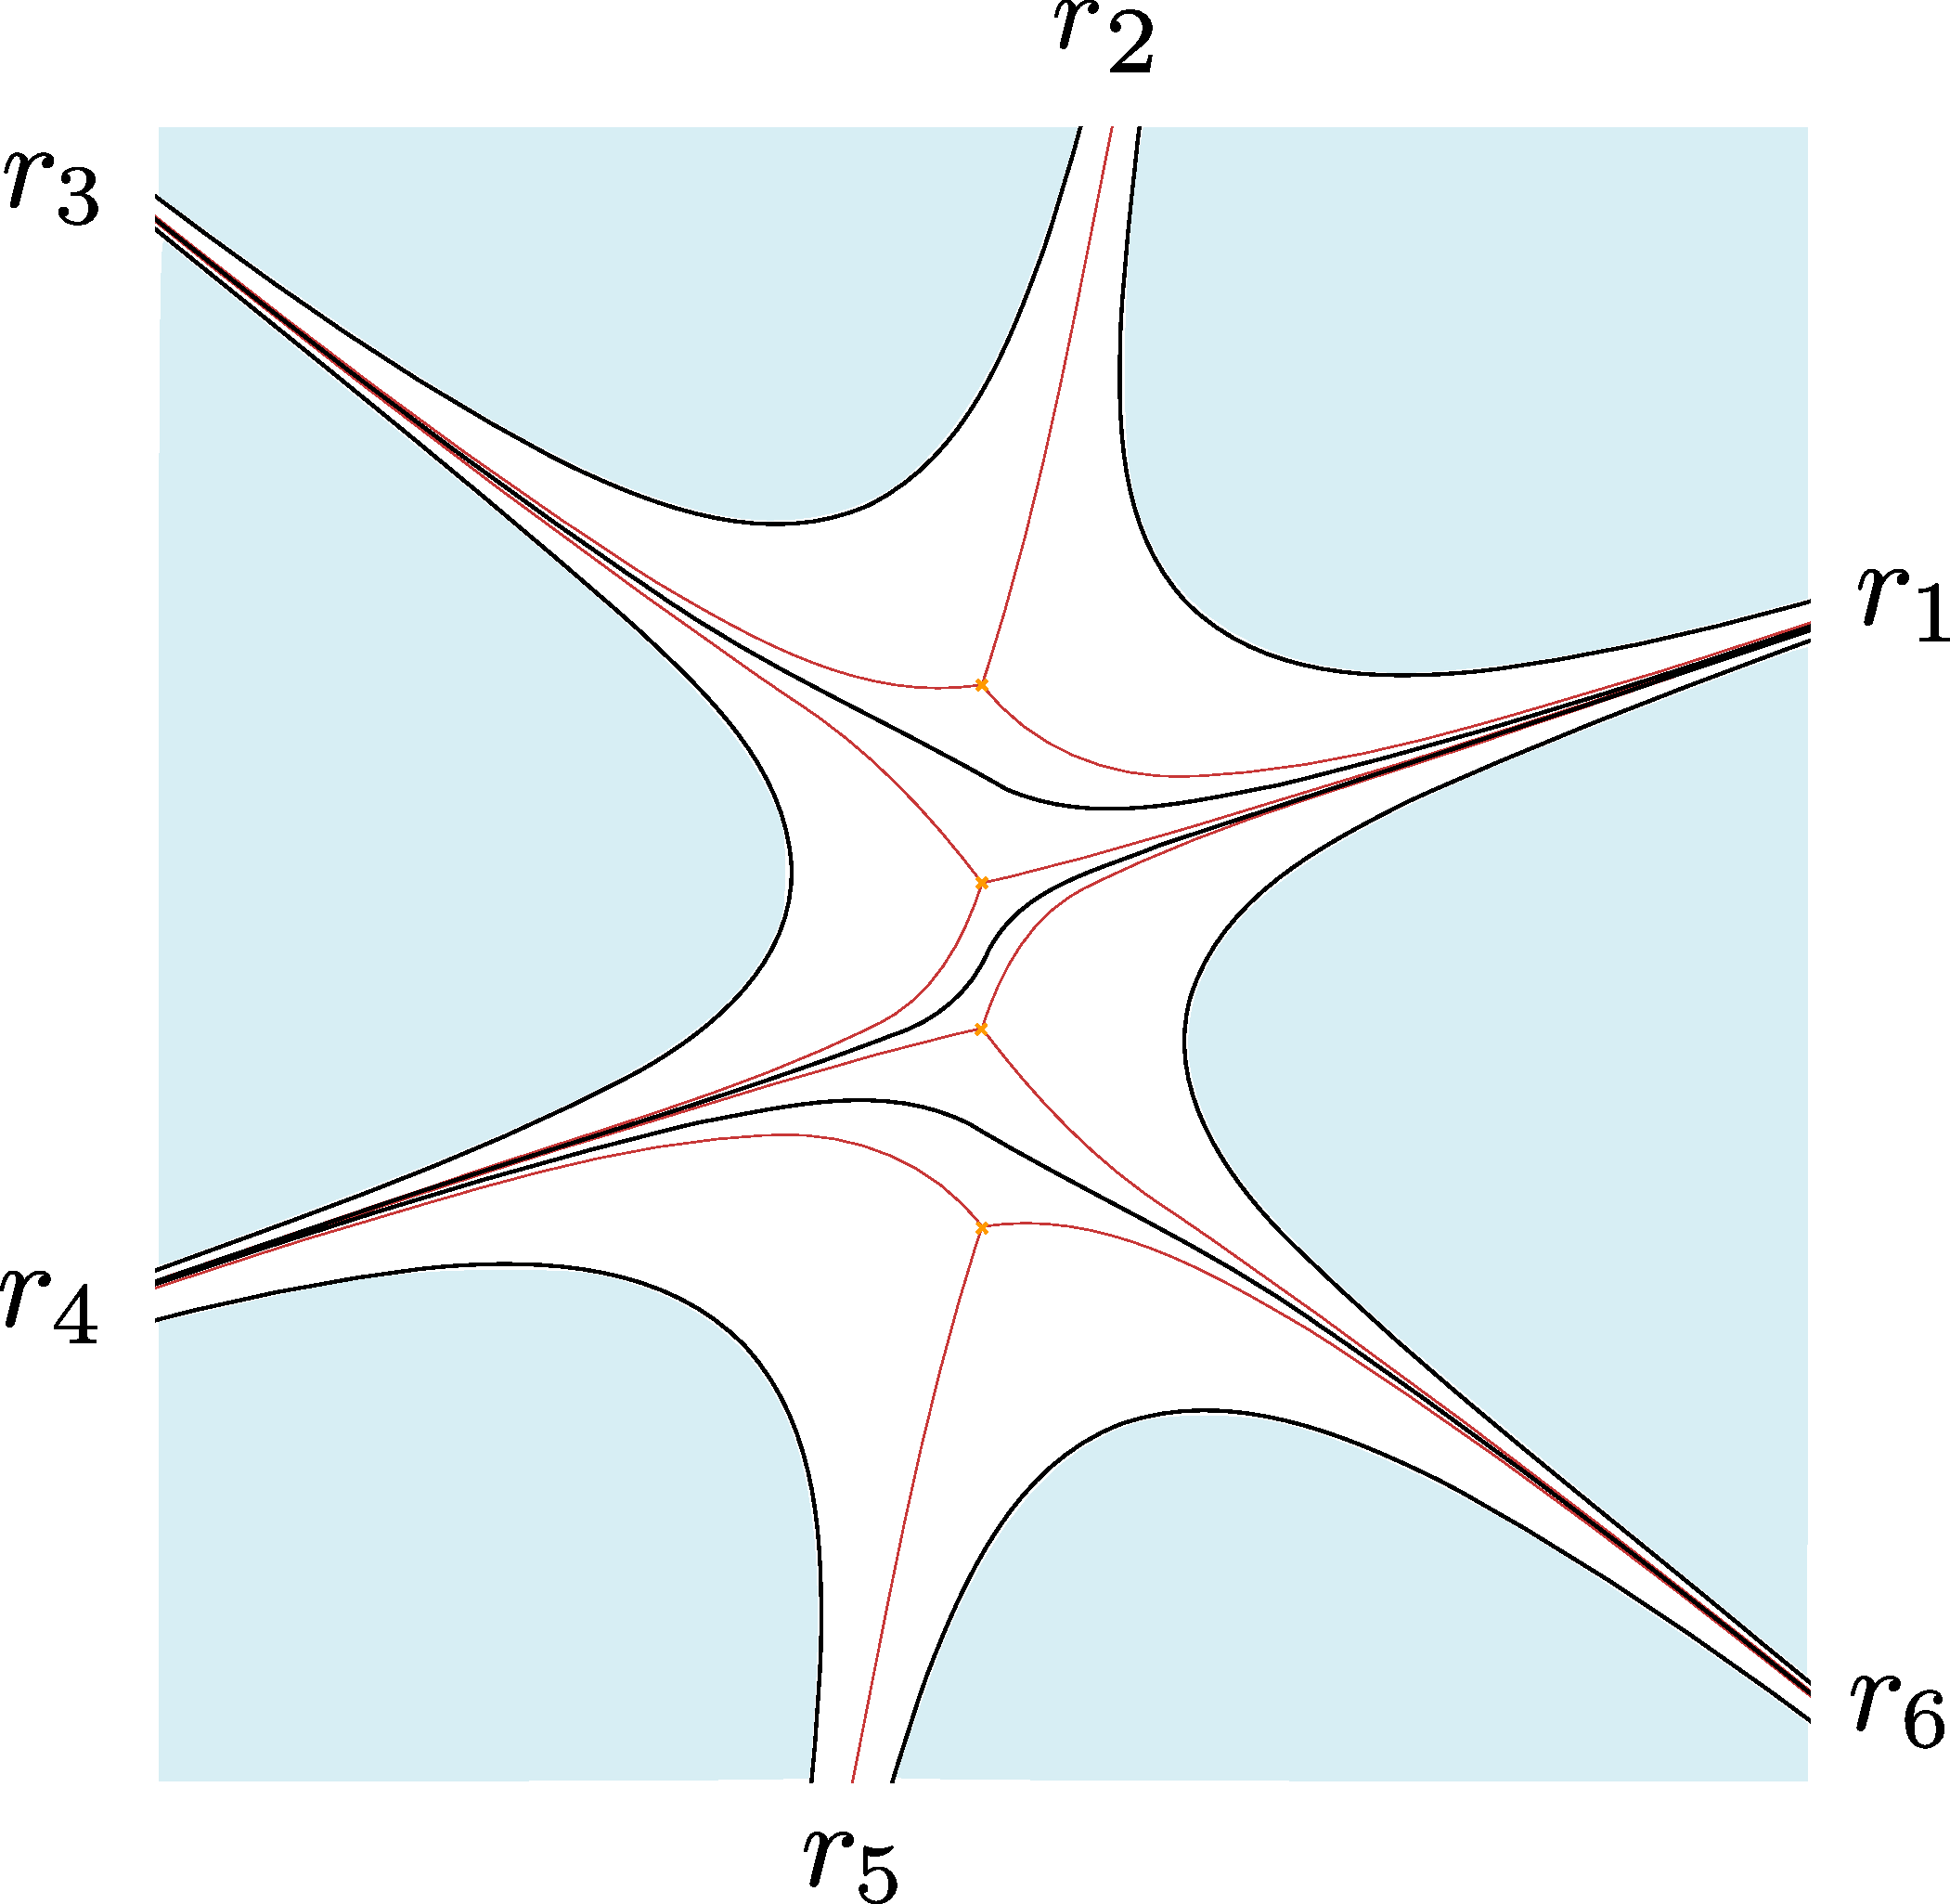
\includegraphics[width=2.75in]{figures/N4plot-crop.pdf}
\caption{$m=0$ 时 $N=4$ 的一个一般 WKB 三角剖分。}\label{fig:N4plot}
\end{minipage}
\hspace{0.4cm}
\begin{minipage}[b]{0.45\linewidth}
\centering 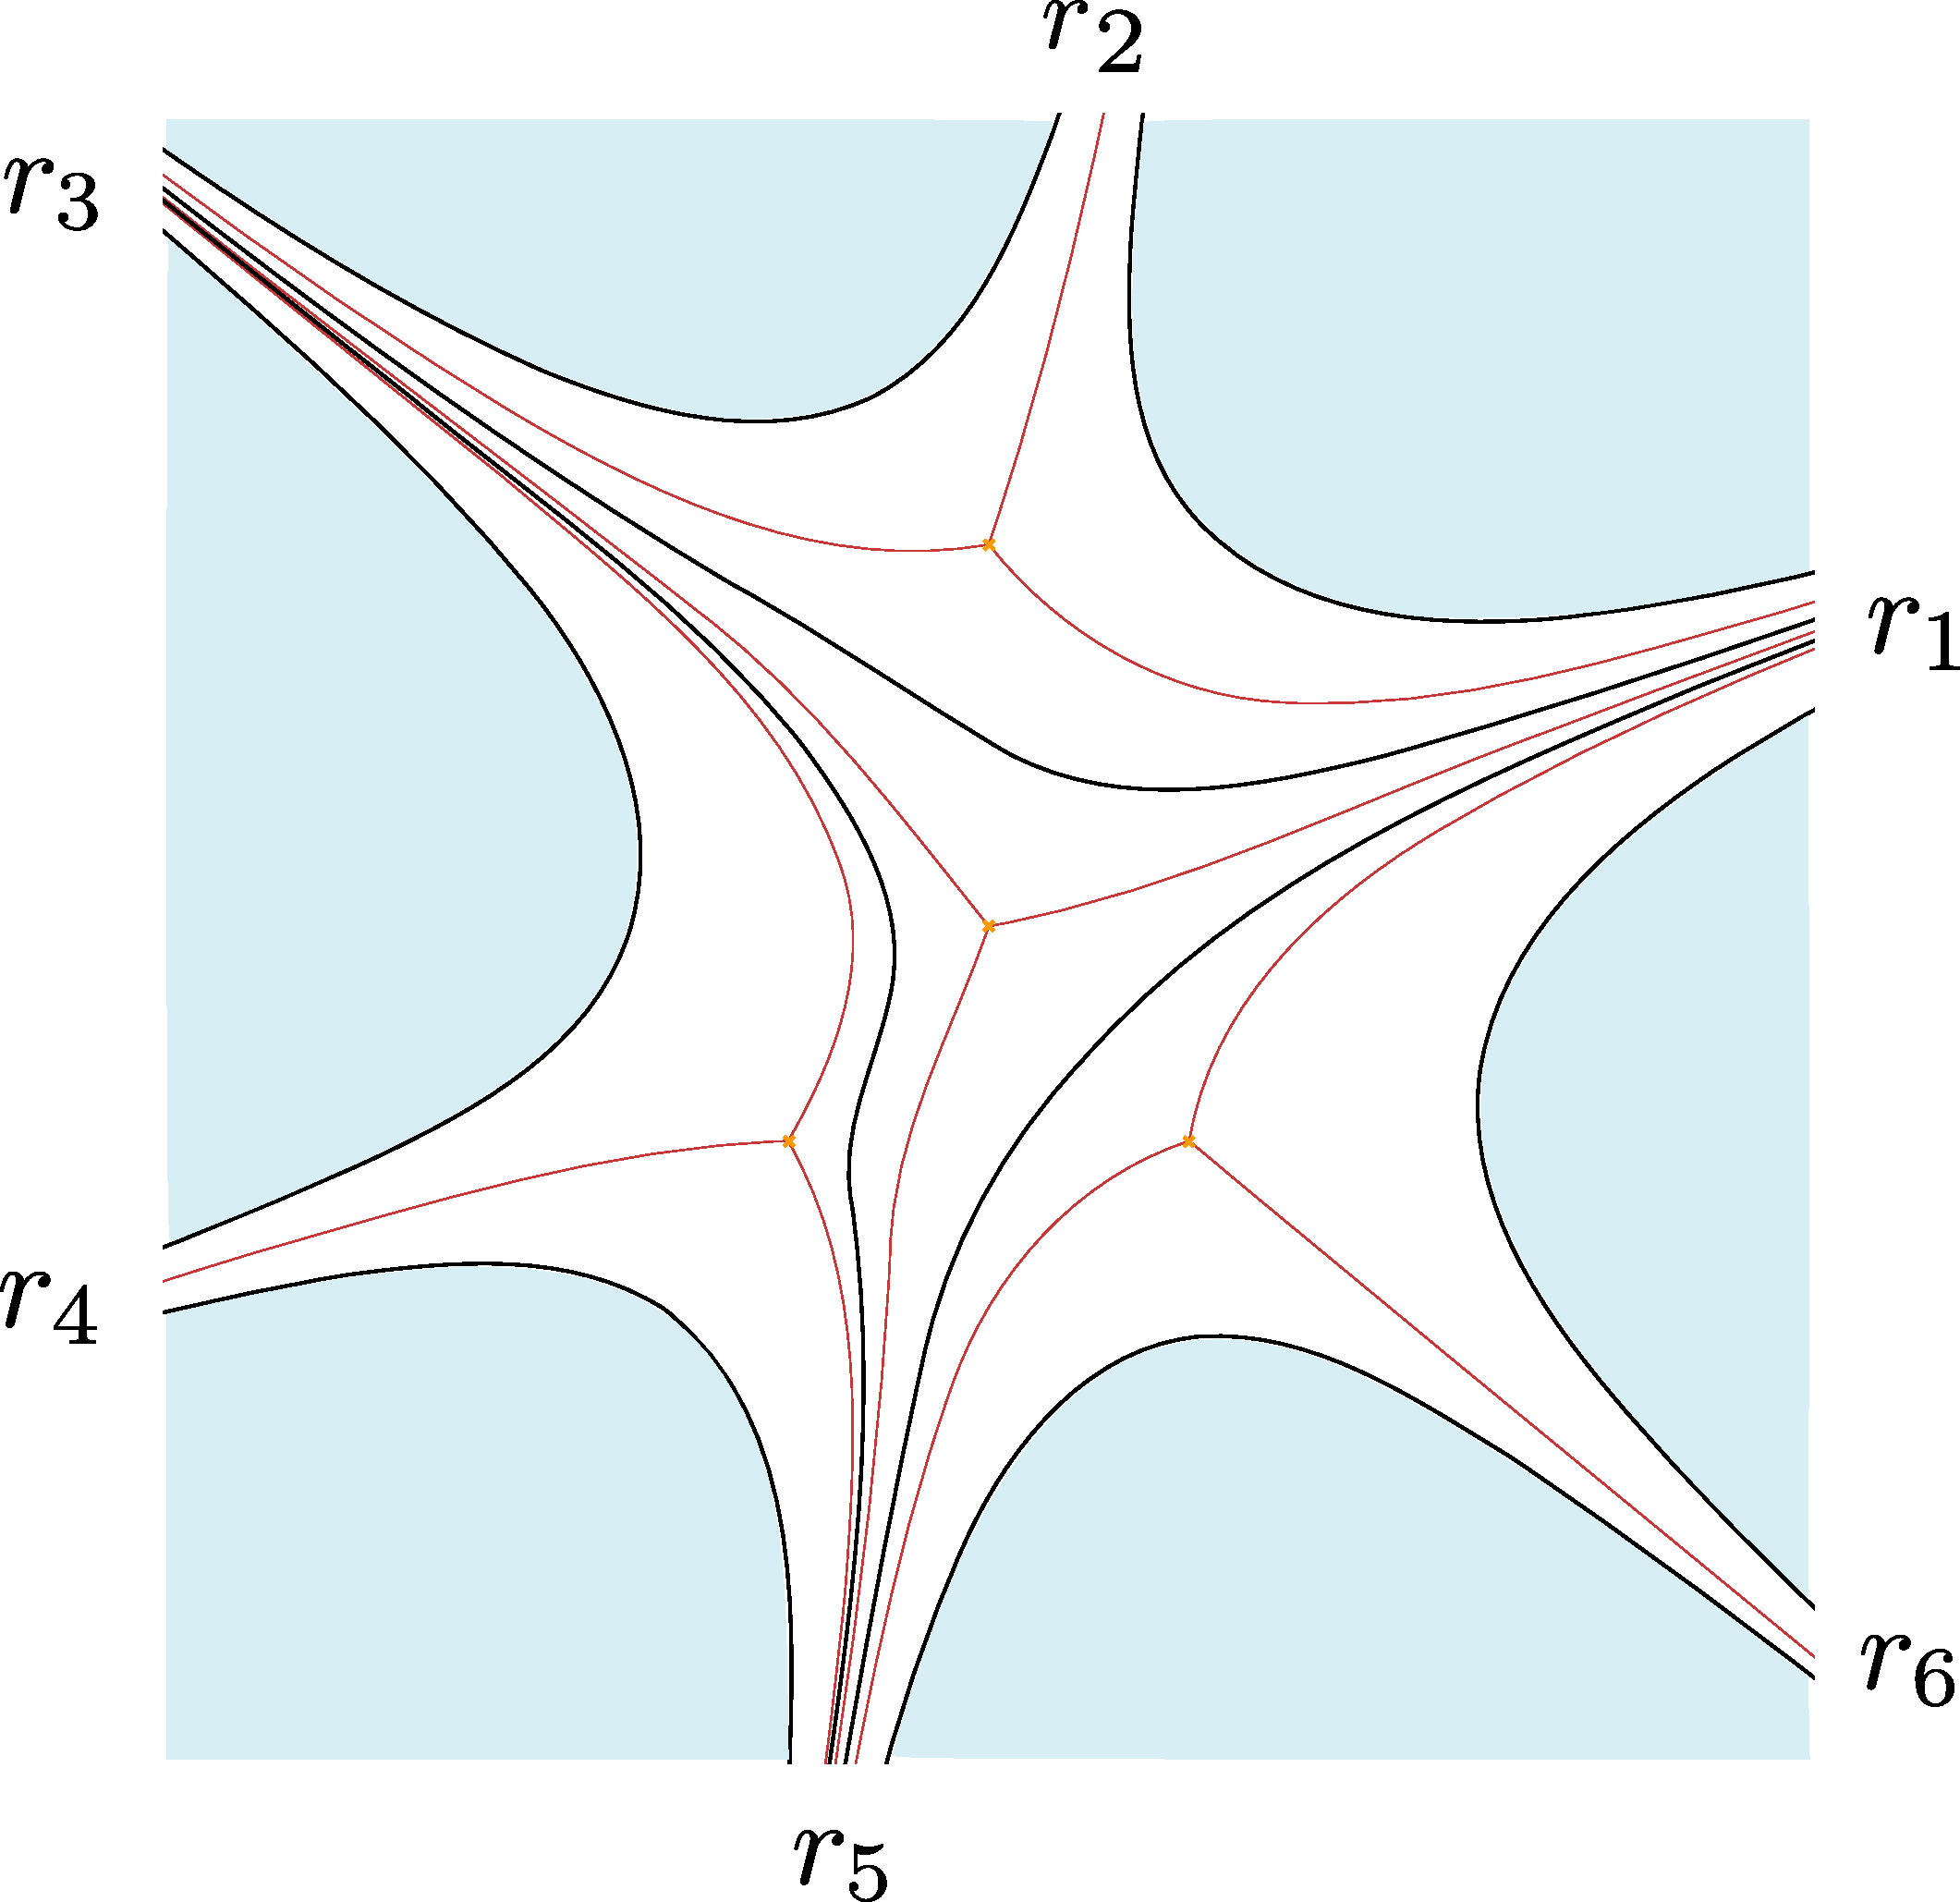
\includegraphics[width=2.75in]{figures/N4plotbis-crop.pdf}
\caption{$m$ 很大时 $N=4$ 的一个一般 WKB 三角剖分。}\label{fig:N4plotbis}
\end{minipage}
\end{figure}

此时 WKB 三角剖分给出的是六边形的三角剖分，如图 50、51 所示。所有可能的三角剖分都会在参数空间的某处出现。
% TODO 合稿改 \ref{fig:N4plot}、\ref{fig:N4plotbis}

下面来描述 BPS 谱。

\subsubsection*{$m=0$ 的情形}

先设 $m=0$ 是有用的。此时判别式退化为 $256 u(u - 4 \Lambda^4)^2$，于是 $\CB$ 中有两个奇点：

\begin{itemize}
\item 在 $u=0$ 处，$P(z)$ 的两个零点在 $z=0$ 处重合，而另外两个零点位于 $z = \pm 2 i \Lambda$。我们预期在这里看到一个 BPS 粒子变为无质量。
\item 在 $u=4 \Lambda^4$ 处，$P(z)$ 是一个完全平方，两对零点在 $z=\pm i \sqrt{2} \Lambda$ 处相撞。我们预期在这里看到两个不同的 BPS 粒子变为无质量。这两个粒子具有相同的规范荷，因为它们在 $\bar\Sigma$ 中对应的闭链同调；但它们的味荷不同。（确实，$\Sigma$ 上这两个对应闭链之差是一个绕 $z = \infty$ 的闭链。若取某个小的 $m \neq 0$，$\oint \lambda$ 就会给出那里单极点的留数 $m$。）
\end{itemize}

通过研究 $\CB$ 中的奇点结构，我们已经遇到了三个 BPS 粒子的效应。现在，让我们沿 $T_\WKB(\vartheta, u)$ 对 $\vartheta$ 的依赖关系，更有系统地考察 BPS 谱。先固定任意一个 $0 < u < 4 \Lambda^4$。此时四个转向点在 $z$-平面中共线，我们会遇到与相邻转向点之间的弦相对应的 BPS 态。把连接中间那两个转向点的 BPS 弦的荷记作 $\gamma_1$。另外两条 BPS 弦的荷记作 $\gamma_2$、$\gamma_3$，于是 $\gamma_2 + \gamma_3$ 是纯味荷（特别地，当 $m=0$ 时 $Z_{\gamma_2} + Z_{\gamma_3} = 0$）。我们取这样的约定：
\begin{equation}
\langle \gamma_3, \gamma_1 \rangle = \langle \gamma_1, \gamma_2 \rangle = 1,
\qquad \langle \gamma_2, \gamma_3 \rangle = 0.
\end{equation}
注意 $\CK_{\gamma_2}$ 与 $\CK_{\gamma_3}$ 对易，这个事实下面会反复用到。$\CB$ 中有一条边缘稳定墙，它穿过这两个奇点，并围住一个椭球状区域；该区域包含线段 $0<u \Lambda^{-4} <4$。\insfig{5.5in}{exa-evolution}{$m=0$ 时的 WKB 三角剖分。上条：在 $u=0$ 处，当 $\vartheta$ 从 $0$ 变到 $\pi$ 时，$T_\WKB$ 的演化很简单，共有三次 flip：在第一条蓝色点线处有一对彼此对易的 flip，在红线处有第三次 flip。下条：对超出边缘稳定墙的 $u$，$T_\WKB$ 以另一种方式演化，涉及六次 flip。在第二条与第四条点线处都发生两次 flip，对应两个荷相同的 BPS 粒子。注意 $T_\WKB(\vartheta)$ 与 $T_\WKB(\vartheta+\pi)$ 相同，只差 WKB 射线的一个重标号。} 现在，通过直接计算（手算或用计算机），就可以得到 $T_\WKB(\vartheta)$ 随 $\vartheta$ 的演化。在图 52 中我们画出了结果，其中取两个 $u$，一个在边缘稳定墙之内、一个在墙外。% TODO 合稿改 \ref{fig:exa-evolution}
在 $u=0$ 处，我们看到 $T_\WKB$ 中有三次 flip，对应三个 BPS 荷 $-\gamma_3$、$\gamma_2$、$\gamma_1$。当我们穿过边缘稳定墙时，中心荷 $Z_{\gamma_2}$、$Z_{-\gamma_3}$ 的相位会与 $Z_{\pm \gamma_1}$ 之一的相位对齐（取哪个符号，取决于我们穿过墙的哪一段）。在墙的另一侧，$T_\WKB$ 中的 flip 以不同的顺序发生，我们一共看到六个 BPS 超多重态。每一对转向点之间都有一条 BPS 弦。

于是，依照与上面 $N=3$ 情形类似的推理，我们必定有穿墙恒等式
\begin{equation} \label{eq:k-identity}
\CK_{\gamma_1} \CK_{\gamma_2} \CK_{-\gamma_3}
= \CK_{\gamma_2} \CK_{-\gamma_3} \CK_{\gamma_1+\gamma_2-\gamma_3} \CK_{\gamma_1+\gamma_2}\CK_{\gamma_1-\gamma_3}
\CK_{\gamma_1}.
\end{equation}
\eqref{eq:k-identity} 中因子的次序很容易理解，只需用到这样的事实：$Z_{\gamma_2} = Z_{-\gamma_3}$，并且当 $k_1, k_2$ 变动时，$Z_{k_1 \gamma_1 + k_2 \gamma_2}$ 的宗量的次序由 $k_1 / k_2$ 的次序决定。同样，人们可以显式检验 \eqref{eq:k-identity} 是一个真正的恒等式，但我们在下一段会给出一个更简单的证明。

\subsubsection*{$m \neq 0$ 的情形}

当 $m \neq 0$ 时，图像要稍复杂一些。对小的 $m$，荷为 $\gamma_2$ 与 $\gamma_3$ 的粒子在 $\CB$ 中略有不同的点处变为无质量。边缘稳定墙也分裂成若干条墙。于是穿墙公式 \eqref{eq:k-identity}「分解」为三个独立的五边形恒等式。一种可能的分解是
\begin{equation}
\begin{split}
\CK_{\gamma_1} \CK_{\gamma_2} \CK_{-\gamma_3}
&= \CK_{\gamma_2} \CK_{\gamma_1+\gamma_2} \CK_{\gamma_1} \CK_{-\gamma_3} \\
&= \CK_{\gamma_2} \CK_{\gamma_1+\gamma_2} \CK_{-\gamma_3} \CK_{\gamma_1-\gamma_3} \CK_{\gamma_1} \\
&= \CK_{\gamma_2} \CK_{-\gamma_3} \CK_{\gamma_1+\gamma_2-\gamma_3} \CK_{\gamma_1+\gamma_2}\CK_{\gamma_1-\gamma_3}
\CK_{\gamma_1},
\end{split}
\end{equation}
它对应三条彼此分离的边缘稳定墙：先是 $Z_{\gamma_1}$ 与 $Z_{\gamma_2}$ 对齐，然后是 $Z_{\gamma_1}$ 与 $Z_{-\gamma_3}$ 对齐，再是 $Z_{-\gamma_3}$ 与 $Z_{\gamma_1 + \gamma_2}$ 对齐。第二种可能是
\begin{equation}
\begin{split}
\CK_{\gamma_1} \CK_{\gamma_2} \CK_{-\gamma_3}
&= \CK_{-\gamma_3} \CK_{\gamma_1-\gamma_3} \CK_{\gamma_1} \CK_{\gamma_2} \\
&= \CK_{-\gamma_3} \CK_{\gamma_1-\gamma_3} \CK_{\gamma_2}\CK_{\gamma_1+\gamma_2} \CK_{\gamma_1} \\
&= \CK_{\gamma_2} \CK_{-\gamma_3} \CK_{\gamma_1+\gamma_2-\gamma_3} \CK_{\gamma_1+\gamma_2}\CK_{\gamma_1-\gamma_3}
\CK_{\gamma_1}.
\end{split}
\end{equation}
相应的 WKB 三角剖分序列如图 53 所示。% TODO 合稿改 \ref{fig:exa-evolution-mass}
\insfig{5.5in}{exa-evolution-mass}{上条：在 $u = 0$ 处，$T_\WKB(\vartheta, u)$ 随 $\vartheta$ 的演化很简单，只经历三次 flip。下条：当我们把 $u$ 变向 $\infty$ 时，会穿过三条墙。每穿过一条墙之后，我们画出 $T_\WKB(\vartheta, u)$ 随 $\vartheta$ 的新演化。在最后一条中，为节省篇幅，我们没有画出规范荷相同的成对 BPS 跳变之间的中间三角剖分。}

在图 54 中，我们画出 $\CB$ 中非常靠近 $Z_{\gamma_1} = 0$ 那个奇点处的墙的结构。墙的整体结构相当复杂，并且依赖于 $m$ 的相位。
% TODO 合稿改 \ref{fig:N4uplane-detail-a}

\insfig{3.3in}{N4uplane-detail-a}{$N=4$ 理论中的边缘稳定墙，画在满足 $Z_{\gamma_1}(u)=0$ 的点 $u$ 附近，取某种小 $m \neq 0$ 的选择。（对 $m$ 的其他相位，图中 $\gamma_2$ 与 $-\gamma_3$ 可能互换。）注意 $\hat\Gamma$ 有单值，因此需要橙色的割线。}

注意，可以沿一条更曲折的路径从小 $u$ 走到大 $u$：这条路径从 $Z_{\gamma_2} = 0$ 与 $Z_{\gamma_3} = 0$ 这两个奇点之间穿过。此时穿墙公式会以另一种方式排列，例如
\begin{equation}
\begin{split}
\CK_{\gamma_3} \CK_{\gamma_1} \CK_{\gamma_2}
&= \CK_{\gamma_1} \CK_{\gamma_1+\gamma_3} \CK_{\gamma_3} \CK_{\gamma_2} \\
&= \CK_{\gamma_1} \CK_{\gamma_2} \CK_{\gamma_1+\gamma_2+\gamma_3}\CK_{\gamma_1+\gamma_3} \CK_{\gamma_3} \\
&= \CK_{\gamma_2} \CK_{\gamma_1+\gamma_2}\CK_{\gamma_1} \CK_{\gamma_1+\gamma_2+\gamma_3}\CK_{\gamma_1+\gamma_3} \CK_{\gamma_3}.
\end{split}
\end{equation}
（记住 $\CK_{\gamma_3}$ 与 $\CK_{\gamma_2}$ 对易。）检验由「从内部区域经不同奇点对之间穿到外部区域」所生成的 BPS 谱，与电荷格绕各奇点自身的单值，二者是否自洽，是一件有趣味的练习。细节随 $m$ 的相位而变。

对 $m$ 作恰当的选择，可以把另一对奇点（比如 $Z_{\gamma_1} = 0$ 与 $Z_{\gamma_2} = 0$）拉到一起，从而在 $\CB$ 中产生一个标度区，看起来就像我们 $N=3$ 的例子。在这个极限下，我们看到一个中心区域，其中的 BPS 谱由下列粒子组成：在复合的 $N=3$ 奇点处变轻的粒子，荷为 $\gamma_2$、$\gamma_1+\gamma_2$、$\gamma_1$；以及在剩下的那个单奇点处变轻的粒子，荷为 $\gamma_3$。我们在图 55 中画出这一 $m$ 选择下 $\CB$ 的结构。$T_\WKB$ 的相应行为见图 56。
% TODO 合稿改 \ref{fig:N4uplane-c}；末句 TODO 改 \ref{fig:N4toN3plot}

\insfig{4.5in}{N4uplane-c}{$N=4$ 理论中的边缘稳定墙，取使奇点 $Z_{\gamma_1}=0$ 与 $Z_{\gamma_2}=0$ 相撞的那个特殊质量 $m$。在每个区域内部，我们按相位的次序（差一个整体的循环置换）列出该区域内谱中所有 BPS 超多重态的荷。在每条墙上，我们给出相应的穿墙公式。}

\insfig{3in}{N4toN3plot}{$N=4$ 理论的三角剖分 $T_\WKB$，其中 $m$ 与 $u$ 取成使三个转向点正在聚拢。在左侧，$N=3$ 例子的五边形结构在 $N=4$ 的三角剖分内部浮现出来。}

对一般的 $m$，在 $\abs{u}$ 足够大的地方有一个区域，那里的转向点大致排成一个正方形，有 6 个 BPS 态与它的边和对角线相关联。从这个行为我们得知：在一个一般的 $\CN=2$ 理论中，在库仑分支上四个转向点汇合的那种奇点附近，我们通常会找到六个轻的 BPS 粒子，它们实现为连接任意一对转向点的 BPS 弦。

\subsection{一般 $N$ 与结合面体}

最后，我们作一些对一切 $N$ 都适用的评述。这些理论中的有限 WKB 曲线已由 Shapere 与 Vafa 在 \cite{Shapere:1999xr} 中描述过，其目的正是研究 BPS 态。他们证明了：

\begin{itemize}
\item 一条有限 WKB 曲线出现的相位 $\vartheta$，由该 WKB 曲线在带穿刺点的平面 $\IC - \{ \CT_i \}$ 中的同伦类唯一决定。

\item 连接任意两个转向点的有限 WKB 曲线至多只有一条。因此 BPS 态只有\emph{有限}多个。

\item 任意两个转向点都可以用有限 WKB 曲线的一段段拼接起来连接（一般每一段的 $\vartheta$ 不同）。因此在库仑分支上任意一点 $u$ 处至少有 $N-1$ 个 BPS 态。

\item BPS 态的最小数目 $N-1$，例如在所有根 $P_N(z)$ 都为实数时达到。最大数目 $\half N (N-1)$，例如在 $P(z) = z^N-1$ 时达到。

\item 自 $N$ 个转向点中的每一个发出的三条分界 WKB 曲线，各自渐近到 $z=\infty$ 处的一条不同射线。

\item 不存在闭合的 WKB 曲线。
\end{itemize}

于是，一般的 WKB 曲线定义了以 $N+2$ 个顶点构成的凸多边形的一个三角剖分。（上面我们已对 $N = 1, 2, 3, 4$ 见过这样的例子。）这一观察开启了一条通往数学中一个丰富分支的联系。$(N+2)$-边形的三角剖分对偶于三价图（trivalent graph），也对应于带 $N+1$ 个终端点的有根二叉树，或等价地，对应于给 $N+1$ 个非结合变量 $x_1 \cdots x_{N+1}$ 的乘积加括号的方式。这类三角剖分的数目是卡塔兰数 $C_N = \frac{1}{N+1} \binom{2N}{N}$。此外，$(N+2)$-边形的三角剖分可以看作一个单纯复形 $\CK_{N+1}$ 的顶点，其中 1-单纯形对应 flip。这个复形就是第 $N$ 个「结合面体」（associahedron），即 Stasheff 多面体的 1-骨架 \cite{MR0158400}。（近期的讨论可参见 \cite{Lee,MR1841954}。）$\CK_3$ 是一条线段，$\CK_4$ 是一个五边形。\cite{MR0158400} 的一个基本引理是：结合面体的面是低维结合面体的乘积。于是特别地，2-胞腔是五边形（对应五边形关系）与四边形（对应「不相交的边上的 flip 彼此对易」这一关系）。另一方面，结合面体本身是单连通的，因此它的二维骨架也是单连通的。\footnote{这一陈述也与范畴论中的 MacLane 相干性定理密切相关 \cite{MR0330253}。} 在我们的语境中，这意味着这些例子里出现的所有穿墙公式都是五边形关系的推论。我们在上面的 $N=3,4$ 例子中已经看到了这一事实。

结合面体在这类例子中的出现，引出了一个问题：$A_\infty$ 代数的理论在这里是否也有有趣的角色可扮演？另一个自然的问题是：若只给出多项式 $P(z)$，是否存在一个计算 BPS 态谱的简单算法？第 11 节% TODO 合稿改 \ref{sec:UniversalStokesMatrix}
中对谱生成元的计算，对第二个问题给出了肯定的回答。

%  GMN2 §10 SU(2) 规范理论：$N_f=0$、$N_f=1$、$N_f=2$ 的第一种实现（原文行 7108–7477）
\section{$SU(2)$ 规范理论}\label{section:SU2Examples}

我们在第 9 节% TODO 合稿改 \ref{section:Superconformal}
中刚刚研究过的那些例子只有 BPS 超多重态，因此当 $\vartheta$ 变化时，WKB 三角剖分
$T_\WKB(\vartheta)$ 只呈现出简单的 flip。接下来我们想考察一些带有 BPS 矢量多重态的例子，
以及与之相应的 \emph{juggle} 变换。我们将研究一组众所周知的理论：带 $N_f=0, 1, 2, 3, 4$
的 $SU(2)$ 规范理论。它们谱的某些方面已经被很好地理解。谱在各种参数区域中的显式结果，
特别可参见 \cite{Bilal:1996sk,Ferrari:1996sv,Ferrari:1997gu}；用 $F$-理论进路的，
可参见 \cite{Banks:1996nj,Douglas:1996js,Gaberdiel:1998mv,Mikhailov:1998bx,DeWolfe:1998bi}。
然而，关于它们的 BPS 谱的完整描述尚不存在。本节将朝着这样一种完整描述取得进展，
给出参数空间许多区域中的谱。事实上，我们的方法可以用来得到模空间任意一点处的谱。

\subsection{$N_f=0$}\label{sec:nf0}

这是 Seiberg--Witten 理论的典型例子。它可以如第 3 节% TODO 合稿改 \ref{sec:physics}
那样，用两根张在两片 NS5-膜之间的 D4-膜构造出来（见方程 (3.130)% TODO 合稿改 \eqref{eq:Standard-SU2-curve}
及其后）。二次微分简单地就是
\begin{equation}
\lambda^2 = \left( \frac{\Lambda^2}{z^3} + \frac{2u}{z^2} + \frac{\Lambda^2}{z} \right) dz^2.
\end{equation}
相应的 Hitchin 系统在 $z=0, \infty$ 处具有可能的最温和的不规则奇点，每个奇点只射出一条
WKB 射线（对应于第 8 节% TODO 合稿改 \ref{sec:irregular}
记号中的 $L=1$）。共有两个转向点，$z_{tp}^\pm = -\frac{u}{\Lambda^2} \pm \sqrt{(\frac{u}{\Lambda^2})^2-1}$，
它们在 $u = \pm \Lambda^2$ 时于 $z_{tp}^\pm = \mp 1$ 处相撞。这两个 $u$ 值是 $\CB$ 中的
奇点。在每个奇点处，都有一个 BPS 粒子变成无质量的。当 $u$ 沿区间 $-\Lambda^2 < u < \Lambda^2$
变化时，两个转向点分开，绕 $z=0$ 朝相反方向运动，然后又重新会合。在该区间上任意一点
（例如 $u=0$）处的 BPS 谱由两个 BPS 超多重态组成。它们由连接两个转向点、但分别从
$z=0$ 处奇点的两侧经过的弦来描述。这两条弦共享两个端点，因此它们的电荷 $\gamma_{1,2}$
满足 $\langle \gamma_1, \gamma_2 \rangle = 2$。$\gamma_{1,2}$ 生成电荷格 $\hat\Gamma$。
$u$ 取在该区间内时典型的 WKB 三角剖分 $T_\WKB(\vartheta,u)$，以及它随 $\vartheta$
变化的变换，见图 57% TODO 合稿改 \ref{fig:Nf0plot}
与图 58% TODO 合稿改 \ref{fig:Nf0evolution-a}
所示。
\insfig{4.2in}{Nf0plot}{带 $N_f=0$ 的 $SU(2)$ 理论的一个典型 $T_\WKB$。为清楚起见，$z=\infty$ 已被映到有限距离。}
\insfig{6in}{Nf0evolution-a}{带 $N_f=0$ 的 $SU(2)$ 理论中 $T_\WKB(\vartheta, u)$ 的演化，$u$ 取在 $u=0$ 附近的强耦合区域。为清楚起见，$z=0$ 与 $z=\infty$ 已被映到有限距离。这里有两次 flip，对应于两个 BPS 态 $\gamma_1$、$\gamma_2$，且 $\langle \gamma_1, \gamma_2\rangle=2$。一条有限 WKB 曲线是红色虚线，另一条是蓝色虚线。红色（蓝色）竖直虚线标示出由于红色（蓝色）BPS 态的存在而引起的 flip。}

$\CB$ 中存在唯一一面椭球形的边缘稳定墙，它穿过那两个奇点。这面墙内部的区域
（我们刚才讨论的正是它）也称为「强耦合」区域，而外部的区域则是弱耦合区域。


注意，本理论中所有的 WKB 三角剖分都不过是两条内部边横穿其间的环带——这正是我们在
第 6.6.3 节% TODO 合稿改 \ref{sec:vector-jump}
中讨论极限三角剖分时所需要的前提情形。当 $u$ 位于强耦合区域时，随 $\vartheta$ 的演化
很简单，如图 58% TODO 合稿改 \ref{fig:Nf0evolution-a}
所示。另一方面，在弱耦合区域中我们会遇到一个新特征，即一个 BPS 矢量多重态。
对适当的 $\vartheta_c$，会出现单参数族的闭合 WKB 曲线，对应于电荷为 $\gamma_1+\gamma_2$
的单个矢量多重态，如图 59% TODO 合稿改 \ref{fig:Nf0plot-limit}
所示。于是，若 $u$ 位于弱耦合区域，则当 $\vartheta$ 的相位变化时，
$T_\WKB(\vartheta,u)$ 会经历无穷多次初等 flip，对应于电荷形如 $(n+1)\gamma_1 + n \gamma_2$
的 BPS 超多重态谱，其 BPS 射线在 $Z_{\gamma_1 + \gamma_2}$ 的相位处聚集。在矢量多重态的
临界相位处，$T_\WKB$ 作一次 \emph{juggle} 变换。随后又是一列无穷多次 flip，对应于电荷形如
$n \gamma_1 + (n+1) \gamma_2$ 的 BPS 超多重态谱。因此我们总共遇到的是该理论标准的弱耦合
BPS 谱：一个电荷为 $\gamma_1+\gamma_2$ 的 W 玻色子，以及一座无穷高的双荷子之塔。

\insfig{4.5in}{Nf0plot-limit}{带 $N_f=0$ 的 $SU(2)$ 理论的极限 WKB 三角剖分。为清楚起见，$z=\infty$ 已被映到有限距离，并画出了几条额外的闭合 WKB 曲线。}

比较这面墙两侧的谱，我们就得到电荷满足 $\langle \gamma_1, \gamma_2\rangle=2$ 时重要的
穿墙公式：
\begin{equation}\label{eq:wcf-prod2}
\CK_{\gamma_1} \CK_{\gamma_2}
= \CK_{\gamma_2} \CK_{\gamma_1+2 \gamma_2}\CK_{2\gamma_1+3\gamma_2} \cdots  \CK_{\gamma_1+\gamma_2}^{-2} \cdots \CK_{3\gamma_1+2\gamma_2}\CK_{2\gamma_1+\gamma_2}\CK_{\gamma_1}.
\end{equation}

更确切地说，这是对这面墙的两个截面之一而言的穿墙公式。对另一个截面，相应的公式是
\begin{equation}
\CK_{\gamma_2}\CK_{-\gamma_1}
= \CK_{-\gamma_1} \CK_{-2\gamma_1+ \gamma_2}\CK_{-3\gamma_1+2\gamma_2} \cdots  \CK_{-\gamma_1+\gamma_2}^{-2} \cdots \CK_{-2\gamma_1+3\gamma_2}\CK_{-\gamma_1+2\gamma_2}\CK_{\gamma_2}.
\end{equation}
同样，只要考虑到奇点周围预期的单值变换，右侧出现的这两个谱是彼此相容的：
\begin{equation}
M_1 = (\gamma_1, \gamma_2) \to (\gamma_1, \gamma_2-2 \gamma_1),
\end{equation}
\begin{equation}
M_2 = (\gamma_1, \gamma_2) \to (\gamma_1+2 \gamma_2, \gamma_2).
\end{equation}


\subsection{$N_f=1$}\label{sec:nf1}

如果在 $SU(2)$ 规范理论中加上一个味，二次微分就变为
\begin{equation}
\lambda^2 = \left( \frac{\Lambda^2}{z^3} + \frac{3u}{z^2}+ \frac{2
\Lambda m}{z} + \Lambda^2 \right) (dz)^2.
\end{equation}
同样，这也可以容易地用第 3 节% TODO 合稿改 \ref{sec:physics}
的方法推出。现在 $z=\infty$ 附近的展开显示出一个带两条 WKB 射线的不规则奇点。
质量参数 $m$ 与该奇点处的留数重合：
\begin{equation}
\lambda \sim \left( \Lambda + \frac{m}{z} + \cdots \right) dz.
\end{equation}

共有三个转向点。若取 $m = 0$，则 $\CB$ 中有三个奇点，位于 $u^3 = \frac{1}{4}
\Lambda^6$ 处。在每个奇点处，都有一个 BPS 态变成无质量的。在 $u=0$ 附近、与这三个奇点
相交的「强耦合」区域中，BPS 谱恰好由这三个 BPS 态组成。它们由连接相邻转向点对、
并绕 $z=0$ 顺时针行进的弦实现。它们的电荷 $\gamma_{1,2,3}$ 构成电荷格 $\hat \Gamma$
的一组基，满足 $\langle \gamma_1, \gamma_2\rangle=\langle \gamma_2, \gamma_3\rangle=\langle
\gamma_3, \gamma_1\rangle=1$。此外，$\sum \gamma_i$ 可以绕过 $z=0$，因而对应于一个
纯味荷。
\insfig{4.5in}{Nf1plot}{带 $N_f=1$ 的 $SU(2)$ 理论的 $T_\WKB$。为清楚起见，$z=0$ 与 $z=\infty$ 已被映到有限距离。}
\insfig{5.5in}{Nf1evolution-a}{带 $N_f=1$ 的 $SU(2)$ 理论中，$T_\WKB(\vartheta, u)$ 随 $\vartheta$ 的演化，$u$ 取在 $u=0$ 附近的强耦合区域。为清楚起见，$z=\infty$ 已被映到有限距离。这里有三次 flip，对应于电荷为 $\gamma_1$、$\gamma_2$、$-\gamma_3$ 的三个 BPS 态。}

当 $m=0$ 时，$Z_{-\gamma_3} = Z_{\gamma_1 + \gamma_2}$，且存在唯一的一面边缘稳定墙，
三个 BPS 态的中心荷在该墙上对齐。这面墙穿过那三个奇点。

我们现在把考查这些例子时一直采用的逻辑颠倒过来。至此，我们一直是根据 $T_\WKB$
对 $\vartheta$ 的依赖来推断 BPS 谱，然后再写出穿过一面墙时出现的那些辛同胚乘积之间的
恒等式。现在反过来，我们要用这些恒等式来确定 BPS 谱必定是什么。

例如，考虑这面墙的一个截面，其上 $Z_{\gamma_1}$、$Z_{\gamma_2}$、$Z_{-\gamma_3}$ 对齐。
在强耦合区域中，当 $\vartheta$ 越过相应的那些相位时，三角剖分经历三次 flip，它们合起来
给出辛同胚 $\CK_{\gamma_1} \CK_{-\gamma_3} \CK_{\gamma_2}$。在另一侧，同一个辛同胚必须
分解为相位按相反次序排列的因子。

为找到这样的分解，我们可以拿已经知道的恒等式来摆弄。把 $\CK_{\gamma_1}$ 搬到右边
毫无问题，只需用两次五边形恒等式
\begin{equation}
\CK_{\gamma_1} \CK_{-\gamma_3} \CK_{\gamma_2} = \CK_{-\gamma_3} \CK_{\gamma_1-\gamma_3}
\CK_{\gamma_2} \CK_{\gamma_1+\gamma_2}\CK_{\gamma_1}.
\end{equation}
然而，各因子仍未按恰当的次序排好：我们需要把 $\CK_{\gamma_2}$ 搬到左边，跨过
$\CK_{-\gamma_3} \CK_{\gamma_1-\gamma_3}$。我们有 $\langle \gamma_1-\gamma_3, \gamma_2 \rangle=2$，
因此需要用我们在 $N_f=0$ 理论中遇到过的恒等式 \eqref{eq:wcf-prod2}（作一次基变换），得到
\begin{multline}
\CK_{-\gamma_3} \CK_{\gamma_1-\gamma_3}\CK_{\gamma_2} \CK_{\gamma_1+\gamma_2}\CK_{\gamma_1}
= \\ \CK_{-\gamma_3} \CK_{\gamma_2} \CK_{2 \gamma_2 +\gamma_1-\gamma_3} \CK_{3 \gamma_2 +2\gamma_1-2\gamma_3}\cdots
\CK_{\gamma_1-\gamma_3+ \gamma_2}^{-2}\cdots \\ \cdots \CK_{2\gamma_2 +3\gamma_1-3\gamma_3}\CK_{\gamma_2 +2\gamma_1-2\gamma_3}\CK_{\gamma_1-\gamma_3} \CK_{\gamma_1+\gamma_2}\CK_{\gamma_1}.
\end{multline}
我们差不多做完了。因子 $\CK_{-\gamma_3}$ 与 $\CK_{\gamma_1+\gamma_2}$ 对应的电荷满足
$Z_{-\gamma_3} = Z_{\gamma_1 + \gamma_2}$，因此在正确重排后的乘积中，它们应当与电荷为
$\gamma_1 - \gamma_3 + \gamma_2$ 的矢量多重态相邻。要把它们搬到那里，我们需要让每一个
都穿过无穷多个其他因子；每一步都用五边形恒等式，最终得到
\begin{multline}
\CK_{\gamma_1} \CK_{-\gamma_3} \CK_{\gamma_2} = \\
\CK_{\gamma_2}\CK_{\gamma_2-\gamma_3} \CK_{2 \gamma_2 +\gamma_1-\gamma_3}\CK_{2 \gamma_2 +\gamma_1-2\gamma_3} \CK_{3 \gamma_2 +2\gamma_1-2\gamma_3}\CK_{3 \gamma_2 +2\gamma_1-3\gamma_3}\cdots
\CK_{-\gamma_3} \CK_{\gamma_1-\gamma_3+ \gamma_2}^{-2} \CK_{\gamma_1+\gamma_2}\cdots \\ \cdots \CK_{2\gamma_2 +3\gamma_1-3\gamma_3}\CK_{2\gamma_2 +3\gamma_1-2\gamma_3}
\CK_{2\gamma_2 +3\gamma_1-2\gamma_3}\CK_{\gamma_2 +2\gamma_1-2\gamma_3}\CK_{2\gamma_1+\gamma_2-\gamma_3}\CK_{\gamma_1-\gamma_3}\CK_{\gamma_1}.
\end{multline}
% 原文此式右侧乘积中 \CK_{2\gamma_2+3\gamma_1-2\gamma_3} 出现了两次，系原文如此，照录。
这确实对应于墙外弱耦合区域中的 BPS 谱。注意，电荷为 $-\gamma_3$ 与 $\gamma_1 + \gamma_2$
的两个「电」超多重态，是带 $N_f=1$ 的 $SU(2)$ 理论的拉氏量中的基本物质粒子，它们具有
相同的规范荷，为 W 玻色子的一半。

当我们在弱耦合区域中改变 $\vartheta$ 时，$T_\WKB$ 经历一列无穷多次 flip，然后作一个
类似于我们在第 6.6.3 节% TODO 合稿改 \ref{sec:vector-jump}
中描述过、并在 $N_f = 0$ 理论中遇到过的「\emph{juggle}」的变换。不过它并不完全相同；
特别是在极限三角剖分中，环带的其中一条边界上有 \ti{两} 个顶点（来自进入 $z=0$ 处奇点的
两条 WKB 射线）。如图 62% TODO 合稿改 \ref{fig:Nf1plot-limit}
所示。这是非一般的情形，它在这里出现是因为我们取了特殊值 $m=0$。这与下述事实有关：跨越
临界 $\vartheta$ 的坐标变换必须是
$\CK_{-\gamma_3} \CK_{\gamma_1-\gamma_3+ \gamma_2}^{-2} \CK_{\gamma_1+\gamma_2}$，
对应于一个矢量多重态加两个超多重态；而在通常情形下，临界 $\vartheta$ 处只有矢量多重态。

\insfig{5in}{Nf1plot-limit}{带 $N_f=1$ 且 $m=0$ 的 $SU(2)$ 理论的极限 $T_\WKB$。为清楚起见，$z=0$ 与 $z=\infty$ 已被映到有限距离，并画出额外的一条闭合 WKB 曲线。}

\insfig{6in}{Nf1plot-limit-pert}{带 $N_f=1$ 且 $m \neq 0$ 的 $SU(2)$ 理论的极限 $T_\WKB$。为清楚起见，$z=0$ 与 $z=\infty$ 已被映到有限距离，并画出额外的一条闭合 WKB 曲线。}

一旦我们把 $m$ 稍微偏离零，就回到一个更常规的格局。当我们从强耦合区域移向大 $u$ 时，
我们所描述的那一列初等操作（或与之非常接近的操作）发生在一列边缘稳定墙上。在很大但
有限的 $u$ 处，与 $\CK_{-\gamma_3}$、$\CK_{\gamma_1+\gamma_2}$ 相联系的那些超多重态的
中心荷，与和 $\CK_{\gamma_1-\gamma_3+ \gamma_2}^{-2}$ 相联系的中心荷并不完全对齐。
因此在重排乘积时，这两个因子 $\CK_{-\gamma_3}$ 与 $\CK_{\gamma_1+\gamma_2}$ 只应移动
有限多步。于是，围绕 $\CK_{\gamma_1-\gamma_3+ \gamma_2}^{-2}$ 的无穷乘积的「核心」，
对应于如第 6.6.3 节% TODO 合稿改 \ref{sec:vector-jump}
中那样的标准 flip 与 \emph{juggle} 序列。极限 WKB 三角剖分如图 63% TODO 合稿改 \ref{fig:Nf1plot-limit-pert}
所示；此时环带的两条边界上都只有一个顶点。

有意思的是把 $m$ 取到 $\frac{3}{2} \Lambda$ 附近，此时 $\CB$ 中有两个奇点合并。我们预期
第 9.4.4 节% TODO 合稿改 \ref{sec:N3}
中的 $N=3$ 理论会在两个奇点附近的标度区域中涌现。确实，看看标度区域中 WKB 叶层化的
形状（如图 64% TODO 合稿改 \ref{fig:Nf1plotN3}
所示），就会看到五边形出现在三个转向点正在汇聚的区域附近，这很有启发性。
\insfig{4.5in}{Nf1plotN3}{带 $N_f=1$ 的 $SU(2)$ 理论的 WKB 三角剖分，其中 $m$ 被调到接近
标度极限，在该极限下第 9.4.4 节% TODO 合稿改 \ref{sec:N3}
的 $N=3$ 理论涌现。}


\subsection{$N_f=2$，第一种实现}

利用第 3 节% TODO 合稿改 \ref{sec:physics}
的膜构造，有两条途径给 $SU(2)$ 规范理论加上第二个味。相应地，存在两个不同的 Hitchin
系统，而它们在 $\CM$ 上的度量预期是相同的。在本小节中我们处理对称的那一种可能性，
此时二次微分为
\begin{equation}
\lambda^2 = \left( \frac{\Lambda^2}{z^4} + \frac{2 \Lambda m_1}{z^3} + \frac{4u}{z^2} +  \frac{2 \Lambda m_2}{z}+ \Lambda^2 \right) dz^2
\end{equation}
于是 $z = 0$ 或 $z = \infty$ 附近的展开都显示出一个带两条 WKB 射线的不规则奇点。
两个质量参数 $m_{1,2}$ 是两个极点处的留数。

共有四个转向点，以及 $\CB$ 中的四个奇点。读者大概会猜到：再一次，$\CB$ 中将存在一个
强耦合区域，其中 BPS 谱只由那四个在四个奇点处无质量的 BPS 粒子组成。

若取 $m_{1,2} = 0$，就会出现一个惊人的简化。带 $N_f = 2$ 理论的 Seiberg--Witten
微分，乃至整个 Hitchin 系统，都可以通过简单的坐标变换 $z^2 \to \hat z$ 映到
$N_f = 0$ 理论的相应对象上。这使我们能够借用在 $N_f = 0$ 情形下的许多讨论。
$N_f = 0$ 理论的每个转向点都映为 $N_f = 2$ 理论的两个转向点；$N_f=0$ 理论的每个
BPS 超多重态都映为 $N_f=2$ 理论中的一对 BPS 超多重态。如图 65% TODO 合稿改 \ref{fig:Nf2plot-a}
所示。这一对超多重态具有相同的规范荷，但它们的味荷不同：两条相应路径之差可以形变为绕 $0$
与绕无穷各走一圈的路径之和。我们把其中一对的电荷记作 $\gamma_1^{1,2}$，另一对记作
$\gamma_2^{1,2}$，并有 $\langle \gamma_1^i, \gamma_2^j \rangle = 1$。此外
$\langle \gamma_1^i, \gamma_1^j\rangle =\langle
\gamma_2^i, \gamma_2^j\rangle =0$。若打开质量，则
$Z_{\gamma_1^1 - \gamma_1^2} = m_1+m_2$，而 $Z_{\gamma_2^1 -
\gamma_2^2} = m_1 - m_2$。

\insfig{3.2in}{Nf2plot-a}{带 $N_f=2$ 的 $SU(2)$ 理论第一种实现、$m_1 = m_2 = 0$ 时一个典型的 WKB 三角剖分。为清楚起见，$z=0$ 与 $z=\infty$ 已被映到有限距离。}
\insfig{3.2in}{Nf2plot-a-limit}{出现矢量多重态的极限 WKB 三角剖分 $T_\WKB(\vartheta_c)$，带 $N_f=2$ 的 $SU(2)$ 理论第一种实现、$m_1 = m_2 = 0$。为清楚起见，$z=\infty$ 已被映到有限距离；图中画出了代表该矢量多重态的单参数族中的两条闭合 WKB 曲线。}

按照这一推理，我们可以猜出相应穿墙公式的形状——它应当是 $N_f = 0$ 的公式
\eqref{eq:wcf-prod2} 的某种加倍，形如
\begin{equation}
\CK_{\gamma^1_1} \CK_{\gamma^2_1} \CK_{\gamma^1_2} \CK_{\gamma^2_2}
= \CK_{\gamma_2}\CK_{\gamma_2} \CK_{\gamma_1+2 \gamma_2}\CK_{\gamma_1+2 \gamma_2} \cdots\ \text{???}\ \cdots \CK_{2\gamma_1+\gamma_2}\CK_{2\gamma_1+\gamma_2}\CK_{\gamma_1}\CK_{\gamma_1}.
\end{equation}
\zy{原文该式右侧此处印作「???」，系作者留下的占位符，未补全；译文照录。}
在右侧，每个 $\gamma_{1,2}$ 究竟代表哪个循环 $\gamma_{1,2}^i$，先验地并不明显，
尽管可以通过考察 WKB 三角剖分中的 flip 来确定。另外，什么应当取代 \emph{juggle}
变换也不明显，因为环绕环状区域的每个圆上都有两个顶点——如图 66% TODO 合稿改 \ref{fig:Nf2plot-a-limit}
所示。当然，我们可以干脆拿已经知道的那些穿墙公式来摆弄，从而完全确定右侧。我们先把
$\CK_{\gamma_1^2}$ 搬到右边，得到
\begin{equation}
\CK_{\gamma_1^1}\CK_{\gamma_1^2} \CK_{\gamma_2^1}\CK_{\gamma_2^2} =
\CK_{\gamma_1^1} \CK_{\gamma_2^1}\CK_{\gamma_2^1+\gamma_1^2}\CK_{\gamma_2^2}\CK_{\gamma_2^2+\gamma_1^2} \CK_{\gamma_1^2},
\end{equation}
% TODO 原文此句作「and then do the same for $\CK_{\gamma_1^2}$」，而后一式实际是对
% $\CK_{\gamma_1^1}$ 作同样的操作；疑原文笔误，照译并在此标注。
然后再对 $\CK_{\gamma_1^2}$ 作同样的操作，得到
\begin{multline}
\CK_{\gamma_1^1} \CK_{\gamma_2^1}\CK_{\gamma_2^1+\gamma_1^2}\CK_{\gamma_2^2}\CK_{\gamma_2^2+\gamma_1^2} \CK_{\gamma_1^2}
= \\ \CK_{\gamma_2^1} \CK_{\gamma_2^1+\gamma_1^1} \CK_{\gamma_2^1+\gamma_1^2} \CK_{\gamma_2^1+\gamma_1^2+\gamma_1^1} \CK_{\gamma_2^2} \CK_{\gamma_2^2+\gamma_1^1}
\CK_{\gamma_2^2+\gamma_1^2}\CK_{\gamma_2^2+\gamma_1^2+\gamma_1^1}  \CK_{\gamma_1^2}  \CK_{\gamma_1^1}.
\end{multline}
我们还需要把 $\CK_{\gamma_2^2}$ 搬到左边，但它会跨过 $\CK_{\gamma_2^1+\gamma_1^2+\gamma_1^1}$，
从而产生一个如同我们在 $N_f = 0$ 例子中遇到过的无穷乘积：
\begin{multline}
\CK_{\gamma_2^1} \CK_{\gamma_2^1+\gamma_1^1} \CK_{\gamma_2^1+\gamma_1^2} \CK_{\gamma_2^1+\gamma_1^2+\gamma_1^1} \CK_{\gamma_2^2} \CK_{\gamma_2^2+\gamma_1^1}
\CK_{\gamma_2^2+\gamma_1^2}\CK_{\gamma_2^2+\gamma_1^2+\gamma_1^1}  \CK_{\gamma_1^2}  \CK_{\gamma_1^1}
= \\ \CK_{\gamma_2^1} \CK_{\gamma_2^1+\gamma_1^1} \CK_{\gamma_2^1+\gamma_1^2} \CK_{\gamma_2^2}\CK_{\gamma_2^1+2\gamma_2^2+\gamma_1^2+\gamma_1^1}\cdots
\CK_{\gamma_2^1+\gamma_2^2+\gamma_1^2+\gamma_1^1}^{-2}\cdots \\ \cdots
 \CK_{2\gamma_2^1+\gamma_2^2+2\gamma_1^2+2\gamma_1^1}\CK_{\gamma_2^1+\gamma_1^2+\gamma_1^1} \CK_{\gamma_2^2+\gamma_1^1}
\CK_{\gamma_2^2+\gamma_1^2}\CK_{\gamma_2^2+\gamma_1^2+\gamma_1^1}  \CK_{\gamma_1^2}  \CK_{\gamma_1^1}.
\end{multline}
因子
$\CK_{\gamma_2^1+\gamma_1^1}\CK_{\gamma_2^1+\gamma_1^2}$ 与
$\CK_{\gamma_2^2+\gamma_1^2}\CK_{\gamma_2^2+\gamma_1^1}$
对应于与矢量多重态 $\CK_{\gamma_2^1+\gamma_2^2+\gamma_1^2+\gamma_1^1}^{-2}$
相位相同的态。因此必须让它们穿过那个无穷乘积，其间用到一列五边形恒等式，最终得到
\begin{multline}
\CK_{\gamma_1^1}\CK_{\gamma_1^2} \CK_{\gamma_2^1}\CK_{\gamma_2^2}
= \\ \CK_{\gamma_2^1}  \CK_{\gamma_2^2}\CK_{\gamma_1^1+\gamma_2^2+\gamma_2^1} \CK_{\gamma_1^2+\gamma_2^2+\gamma_2^1}\CK_{\gamma_1^2+\gamma_1^1+\gamma_2^2+2\gamma_2^1}
\CK_{\gamma_1^2+\gamma_1^1+\gamma_2^1+2\gamma_2^2}\cdots \\ \cdots\CK_{\gamma_2^1+\gamma_1^1} \CK_{\gamma_2^1+\gamma_1^2}
\CK_{\gamma_2^1+\gamma_2^2+\gamma_1^2+\gamma_1^1}^{-2}\CK_{\gamma_2^2+\gamma_1^1}
\CK_{\gamma_2^2+\gamma_1^2} \cdots \\ \cdots \CK_{\gamma_1^2+2\gamma_1^1+\gamma_2^2+\gamma_2^1}
\CK_{2\gamma_1^2+\gamma_1^1+\gamma_2^2+\gamma_2^1}\CK_{\gamma_1^2+\gamma_1^1+\gamma_2^1} \CK_{\gamma_1^2+\gamma_1^1+\gamma_2^2}  \CK_{\gamma_1^2}  \CK_{\gamma_1^1}.
\end{multline}
与 $N_f = 1$ 的例子一样，若打开 $m_{1,2} \neq 0$，那唯一的一面墙就会碎成若干面墙。
在这些参数上玩一玩，可以得到一些有趣的结果。例如，若取 $m_1 = m_2 = 2 \Lambda$，
我们就得到一个漂亮的例子，
\begin{equation}
\lambda^2 = \left( \frac{\Lambda^2(z+1)^4}{z^4} + \frac{16 \tilde u}{z^2} \right) dz^2,
\end{equation}
其中 $\CB$ 的四个奇点里有三个在 $\tilde u = 0$ 处合并，并且我们能够恢复 $N=4$
Argyres--Douglas 标度极限。强耦合区域中四个粒子之一变得非常重，而另外三个与 $N=4$
Argyres--Douglas 理论的基本谱重合。

% ---------------------------------------------------------------------
% §10.4 插叙（原文 7479–7509 行；BRIEF 行段未覆盖，合稿时补译）
% ---------------------------------------------------------------------
\subsection{插叙：非阿贝尔味对称与 WKB 三角剖分} \label{subsec:intermission-flavor}

我们在第 3.2.8 节已经注意到% TODO 合稿改 \ref{sec:flavor}，当正则奇点 $\CP$ 处的质量参数趋于零、非阿贝尔 $SU(2)$ 味对称被恢复时，WKB
流线会有什么样的行为。考虑该极限下整片 WKB 叶状结构的行为是有益的。当 $m \to 0$ 时，一个转向点
$\CT$ 向 $\CP$ 移动。在一般的 $\vartheta$ 处，从 $\CT$ 出发的三条分离 WKB 曲线中有一条流向
$\CP$。另外两条朝相反方向绕过 $\CP$，然后彼此靠得很近地流走，最终落到某个别的奇点上。
（于是 $T_\WKB$ 是退化的，只有一条边从 $\CP$ 伸出。）

随着 $\vartheta$ 变化，我们偶尔会遇到相位非常接近的一对 BPS 态，此时这两条分界线变成有限
WKB 曲线并落到另一个转向点 $\CT'$ 上。这两个 BPS 态的电荷相差（两倍的）一个绕奇点的圈。
换言之，这些有限 WKB 曲线代表一对电荷为 $\gamma \pm \gamma_+$ 的 BPS 粒子二重态，其中
$\gamma_+$ 是与奇点 $\CP$ 相联系的味荷。

对处于 $Z_{\gamma \pm \gamma_+}$ 的相位之间那个狭窄窗口里的 $\vartheta$，这两条分界线从转向点
$\CT'$ 的两侧经过，并走向不同的奇点。WKB 三角剖分的相应变换是直截了当的。第一个 BPS 态
引起与 $\CP$ 相联系的退化三角形的非退化边发生一次 flip。于是有两条边终止于 $\CP$。第二个
BPS 态引起终止于 $\CP$ 的那条旧边发生一次 flip，于是我们又得到退化三角形。
\insfig{4.5in}{flavor-evolution}{当 $SU(2)$ 破缺质量很小时，$T_\WKB$ 中与一个 $SU(2)$ 味双重态
BPS 超多重态相关的两次 flip。}

% =====================================================================
%  GMN2 §10.5–10.7  $N_f=2$ 的第二种实现 / $N_f=3$ / $N_f=4$：超共形情形
%  原文：wkb-paper.tex 7512–7872 行；PDF（印刷）p.132–140
%  编号公式 (10.18)–(10.30) 共 13 条（其中 (10.20)、(10.29) 原为 multline，
%  (10.23)、(10.26) 原为 align，均改写为 equation+split/aligned，各占一个式号）；
%  插图 7 幅（图 68–74，图号按原文计数硬编码，每处留 % TODO）；脚注 0 条
%  【归属】§10.4「Intermission」（原文 7479–7509 行）不在本块行段内，故未收录
%  （BRIEF 把 7108–7511 行划给 ch14）；若 ch14 也未收，合稿时需补。
%  跨块引用：第 3 节、第 3.2.8 节、第 11 节暂写硬编码并加 % TODO
% =====================================================================

\subsection{$N_f=2$：第二种实现} \label{subsec:Nf2second}

接下来我们考虑 $N_f=2$ 理论的非对称实现：其中 $z=\infty$ 处的不规则奇点与 $N_f=0$ 理论中的相同，而 $z=0$ 处的不规则奇点则被两个正则奇点取代：
\begin{equation}
\lambda^2 = \frac{P_3(z)}{z^2 (z-1)^2} = \left( \frac{m_+^2}{z^2}+\frac{m_-^2}{(z-1)^2} + \frac{\Lambda^2 +u}{2 z} + \frac{\Lambda^2 -u}{2 (z-1)} \right) dz^2
\end{equation}
这里参数 $u,\Lambda$ 未必与上一小节中的相同。绕 $z=\infty$ 的展开显示出一个带单条 WKB 射线的不规则奇点。共有三个转向点，而 $\CB$ 中共有四个奇点。

当质量 $m_\pm$ 非常小时，这里典型的 $T_\WKB$ 有两个退化三角形附着在 $z=\infty$ 处的奇点上。强耦合谱只包含两对 BPS 态，每个奇点一对，如图 68 所示。
% TODO 合稿改 \ref{fig:Nf2evolution-a}
\insfig{5.5in}{Nf2evolution-a}{$N_f=2$ 理论第二种实现的 WKB 三角剖分的演化：取小 $m_\pm$，位于 $u=0$ 附近的强耦合区。为清楚起见，$z=\infty$ 已被映到有限距离处。图中有两对 flip，对应荷为 $\gamma^i_1$、$\gamma^i_2$ 且满足 $\langle \gamma^i_1,\gamma^j_2\rangle=1$ 的两个 BPS 态。注意中间两幅图相差一个 pop，而 pop 并不对应任何 BPS 态。}

与上一节（或第 3 节的分析）相比较可知 $m_\pm = m_1 \pm m_2$。弱耦合谱则表现为一列成对的 BPS 态，它们或与 $z=0$ 处的奇点、或与 $z=1$ 处的奇点相关联（如上一节所述），并产生紧密缠绕的退化三角形。对一般的 $m_\pm$，可能出现退化程度较低的三角剖分，如图 69 所示。
% TODO 上面「第 3 节」合稿改 \ref{sec:physics}
% TODO 合稿改 \ref{fig:Nf2plot-b}
\insfig{2.5in}{Nf2plot-b}{$N_f=2$ 理论（第二种实现）在一般质量下的一个典型 WKB 三角剖分。为清楚起见，$z=\infty$ 已被映到有限距离处。}

$N_f=2$ 理论的两种实现所对应的两个\hk 度量完全相同，这一点绝非显然。事实上，这正是第 3.2.8 节那个出人意料的同构的一个例子。「$N_f=2$ 的两个 Hitchin 系统具有同一个\hk 度量」这一命题的证明如下：这两个系统有相同的谱曲线（尽管它们在 $T^* \IC \IP^1$ 中的嵌入方式不同），也有相同的中心荷函数。现在假设我们能证明（比方说，通过显式考察 $T_\WKB$）：两个系统中的 BPS 谱在某个强耦合点处重合。那么穿墙公式保证两个谱在整个 $\CB$ 上一致；此外，函数 $\CX^\vartheta_\gamma$ 也必然一致，因为它们是同一个黎曼–希尔伯特问题的解，且具有相同的渐近行为。于是这两个 Hitchin 系统的扭量空间与\hk 度量都必定相同。
% TODO 上面「第 3.2.8 节」合稿改 \ref{sec:surprise}

\subsection{$N_f=3$} \label{subsec:Nf3}

带 $N_f=3$ 的 $SU(2)$ 规范理论对应一个 $SU(2)$ Hitchin 系统，它与 $N_f=2$ 理论的第二种实现颇为相似。二次微分为
\begin{equation}
\lambda^2 = \frac{P_4(z)}{z^2 (z-1)^2} = \left(
\frac{m_+^2}{z^2}+\frac{m_-^2}{(z-1)^2} + \frac{2\Lambda m +u}{2 z}
+ \frac{2 \Lambda m -u}{2 (z-1) } + \Lambda^2\right) dz^2
\end{equation}
绕 $z=\infty$ 的展开显示出一个带两条 WKB 射线的不规则奇点，见图 70。
% TODO 合稿改 \ref{fig:Nf3plot}
\insfig{2.5in}{Nf3plot}{带 $N_f=3$ 的 $SU(2)$ 理论的一个典型 WKB 三角剖分。为清楚起见，$z=\infty$ 已被映到有限距离处。}

$z$-平面上有四个转向点，而 $\CB$ 中有五个奇点。三个质量参数 $m$、$m_\pm$ 的地位并不相同。（若要对称地处理它们，就得用 $SU(3)$ Hitchin 系统来实现该理论，这超出了本文的范围。）

当 $m$ 与 $m_\pm$ 都非常小时，$\CB$ 中有四个奇点在 $u=0$ 附近聚拢。在这四个奇点处变为无质量的 BPS 粒子具有相同的规范荷，但味荷不同。见图 71。
% TODO 合稿改 \ref{fig:Nf3evolution-a}
\insfig{5.5in}{Nf3evolution-a}{$N_f=3$ 理论中 $T_\WKB(\vartheta)$ 的演化：取小 $m$ 与 $m_\pm$，位于 $\CB$ 中 $u=0$ 附近的强耦合区。为清楚起见，$z=\infty$ 已被映到有限距离处。随 $\vartheta$ 变化共出现五次 flip，对应荷为 $\gamma^i_1$、$\gamma_2$ 且满足 $\langle \gamma^i_1,\gamma_2\rangle=1$ 的 BPS 态。第二幅与第三幅图相差一个 pop，而 pop 并不对应任何 BPS 态。}

我们知道，当 $m_\pm$ 足够小时，每个正则奇点附近都会有一个转向点；而 BPS 态通常以 $SU(4)$ 味对称的相应 $SU(2)_\pm$ 子群的二重态形式出现。$m$ 则是剩下的那个 $U(1)\in SU(4)$ 的质量参数。这四个粒子实际上构成 $SU(4)$ 的一个 ${\bf 4}$ \cite{Seiberg:1994aj}。的确，在 $SU(2)\times SU(2)\times U(1)$ 之下 ${\bf 4}$ 分解为 $({\bf 2},{\bf 1})_{+1}\oplus({\bf 1},{\bf 2})_{-1}$。从图 71 可以看出，这两个二重态的荷确实相差一个无穷远处的味荷。
% TODO 合稿改 \ref{fig:Nf3evolution-a}

在 $u\sim \frac{\Lambda^2}{4}$ 处还有第二个奇点，那里两个转向点汇合。总而言之，存在一个包含区间 $0<u<\frac{\Lambda^2}{4}$ 的强耦合区，其 BPS 谱很简单：荷为 $\gamma_1^i$ 的粒子的四重态（它们的规范荷全都相同），外加单个荷为 $\gamma_2$、满足 $\langle \gamma_1^i,\gamma_2\rangle=1$ 的粒子；此外对所有 $i,j$ 都有 $\langle \gamma_1^i,\gamma_1^j\rangle=0$。于是穿墙公式就预言了弱耦合区中已知的正确谱——只要把我们先前列出的那些恒等式按一个简单但冗长的次序用一遍，就能看出来。为写出最终结果，令 $\tilde\gamma = 2\gamma_2+\gamma_1^1+\gamma_1^2+\gamma_1^3+\gamma_1^4$。于是：
\begin{equation}
\begin{split}
&\left( \prod_{i=1}^4 \CK_{\gamma_1^i}\right) \CK_{\gamma_2} =
\CK_{\gamma_2} \left( \prod \CK_{\gamma_2+\gamma_1^i}\right) \CK_{\gamma_2+\tilde \gamma}\left( \prod \CK_{\tilde \gamma-\gamma_1^i}\right) \cdots \\
&\quad \cdots \CK_{2\gamma_2+\gamma_1^1+\gamma_1^2+\gamma_1^3+\gamma_1^4}^{-2} \left(\prod_{i<j}\CK_{\gamma_2+\gamma_1^i+\gamma_1^j}\right) \cdots \\
&\quad \cdots \left( \prod \CK_{\tilde \gamma-\gamma_2-\gamma_1^i}\right)\CK_{\tilde \gamma-\gamma_2}\left( \prod_{i=1}^4 \CK_{\gamma_1^i}\right).
\end{split}
\end{equation}

\subsection{$N_f=4$：超共形情形} \label{subsec:SuperConformalCase}

最后，我们已有足够的准备来正经讨论 $N_f=4$ 理论了。本小节只考虑该理论的「平衡」（balanced）实现：$\IC\IP^1$ 上有四个正则奇点和四个转向点。\SW 曲线形如
\begin{equation}
\lambda^2 = \frac{P_4(z)}{D_4(z)^2}(dz)^2= \frac{P^0_4(z)+ u
D_4(z)}{D_4(z)^2}(dz)^2.
\end{equation}
第二个等号中我们引入了一个基点，并定义了一个可归一化的 $u$ 参数。除 $u$ 之外，该理论还有四个质量参数和一个恰好边缘（exactly marginal）的规范耦合。$u$-平面 $\CB$ 中共有 $6$ 个奇点。

若所有质量都取零（或 $u$ 远大于各质量），WKB 流可以变得非常复杂。在这一区域，由 $\lambda$ 决定的 WKB 流可以被下面这个 $\lambda_0$ 的 WKB 流很好地逼近：
\begin{equation}
\lambda_0=\frac{dz}{\sqrt{D_4(z)}} = d\upsilon,
\end{equation}
其中 $\upsilon$ 是椭圆曲线 $y^2=D_4(z)$ 上的单值化坐标（uniformizing coordinate）；于是这些流不过是环面上的直线，其倾角由 $\vartheta$ 决定。对任何有理斜率，我们都得到闭合的 WKB 曲线。特别地，存在一个由 $W$-玻色子构成的无穷谱，它们组成一个 $SL(2,\IZ)$ 对偶轨道。

在 $W$-玻色子出现的同一个 $\vartheta$ 处，还应当出现八个超多重态，它们处于 $Spin(8)$ 味对称群的表示 ${\bf 8}_v$、${\bf 8}_s$ 或 ${\bf 8}_c$ 之中。我们可以这样来理解它们：由于考虑的是非常小的质量，每个转向点都紧挨着四个正则奇点之一。于是，连接两个转向点的 BPS 超多重态会以二重态的形式出现，分别属于两个端点所对应的两个 $SU(2)$ 味子群。若把这四个奇点记作 $a,b,c,d$，把 $Spin(8)$ 中相应的子群记作 $SU(2)_a$、$SU(2)_b$、$SU(2)_c$、$SU(2)_d$，则我们有如下分解
\begin{equation}
\begin{aligned}
{\bf 8}_v &= ({\bf 2}_a, {\bf 2}_b, {\bf 1}_c, {\bf 1}_d) \oplus ({\bf 1}_a, {\bf 1}_b, {\bf 2}_c, {\bf 2}_d), \\
{\bf 8}_s &= ({\bf 2}_a, {\bf 1}_b, {\bf 2}_c, {\bf 1}_d) \oplus ({\bf 1}_a, {\bf 2}_b, {\bf 1}_c, {\bf 2}_d), \\
{\bf 8}_c &= ({\bf 2}_a, {\bf 1}_b, {\bf 1}_c, {\bf 2}_d) \oplus ({\bf 1}_a, {\bf 2}_b, {\bf 2}_c, {\bf 1}_d).
\end{aligned}
\end{equation}
每条闭合 WKB 曲线都把四个奇点分成两对，或是 $(ab,cd)$，或是 $(ac,bd)$，或是 $(ad,bc)$。相应的那对转向点（比方说 $(ab,cd)$）承载着（比方说）${\bf 8}_v$ 中的那 8 个 BPS 超多重态。

一旦打开有限的质量参数，谱就大为简化：每个奇点都变成一个吸引子，使绝大多数闭合 WKB 曲线不再出现。事实上，借助下面的写法引入另一个辅助环面是件有趣的事：
\begin{equation}
\lambda = \frac{dz}{\sqrt{P_4(z)}}\frac{P_4(z)}{D_4(z)}= d\upsilon
\frac{P_4(z)}{D_4(z)},
\end{equation}
其中 $d\upsilon = dz/\sqrt{P_4(z)}$ 现在是环面 $y^2=P_4(z)$ 的单值化参数。WKB 曲线提升为该环面上亚纯微分 $\lambda$ 的流线。$P_4$ 的每个零点在环面上变成一个二重零点，而 $D_4$ 的每个零点则提升为一对极点。若质量参数很小，这对极点会非常靠近那个二重零点。流的局部图像显示出一处局域扰动，它对流而言有一个定义良好的「吸收截面」。我们甚至可以把这个截面算出来：对 $\lambda$ 的局部形式积分，
\begin{equation}
w = \int \lambda \sim \int_{\upsilon=0}^{\upsilon} \frac{m
(\upsilon')^2}{1-(\upsilon')^2}d\upsilon' = - m \upsilon +
\frac{m}{2}\log \frac{1+\upsilon}{1-\upsilon}.
\end{equation}
由于 $- m \upsilon + \frac{m}{2}\log
\frac{1+\upsilon}{1-\upsilon}\sim \frac{m}{3}\upsilon^3 + \cdots$，从 $\upsilon=0$ 发出六条满足 ${\rm Im}(e^{-i \vartheta} w) =0$ 的流。渐近到平行直线的那些流，其间距为 $\pi \mathrm{Re}\left( e^{-i \vartheta}m \right)$。见图 72。
% TODO 合稿改 \ref{fig:perturbed-flow}
\insfig{2.5in}{perturbed-flow}{环面上 $\lambda$ 的一群零点与极点附近的局部流。}

无论质量参数多小，只要一条 WKB 曲线绕环面缠绕足够多次，该奇点最终必定会把它吸住——除非 $\vartheta$ 非常接近质量参数的相位。因此，除非所有质量参数的相位都对齐，看起来在有限的 $u$ 处只有有限多个 $W$-玻色子的 $SL(2,\IZ)$ 像能够存活下来。适当调节质量参数，甚至应当能找到一个没有任何矢量多重态 BPS 态存活的「强耦合区」。那显然会是我们展开分析的好起点。

有鉴于此，让我们考虑下面这个对称的参数选取：
\begin{equation}
\begin{split}
\lambda^2 &= \frac{z^4-u(z^4-1)}{(z^4-1)^2} = \\
&= \frac{1}{16 (z-1)^2}-\frac{1}{16 (z-i)^2}-\frac{1}{16 (z+i)^2}+\frac{1}{16 (z+1)^2}+\frac{1-4 u}{16 (z-1)}\\
&\quad -\frac{i (4 u-1)}{16 (z-i)}+\frac{i (4 u-1)}{16 (z+i)}+\frac{4 u-1}{16 (z+1)}.
\end{split}
\end{equation}
我们把规范耦合调到 $\tau=i$，这给问题带来一个有用的离散 ${\mathbb Z}_4$ 对称性。奇点为 $z_a = 1$、$z_b = i$、$z_c = -1$、$z_d = -i$。质量参数算出来是 $m_a = \frac{1}{4} z_a$。它们的符号是任意的：对这一套参数，我们采用的约定是 $\sum m_a=0$。图 73 给出了一个 WKB 三角剖分的例子。
% TODO 合稿改 \ref{fig:Nf4plot}
\insfig{3.0in}{Nf4plot}{$N_f=4$ 的 $SU(2)$ 理论在特殊 ${\mathbb Z}_4$ 对称点处的一个典型 WKB 三角剖分。}

${\mathbb Z}_4$ 对称性保证 $u$-平面上的六个奇点三三聚拢，在 $u=0$ 与 $u=1$ 处给出两个 $N=4$ 型的奇点。当 $u$ 趋近这两个点时，转向点分别汇合于 $z=0$ 或 $z=\infty$。我们知道，每个 $N=4$ 奇点附近应当有 $6$ 个轻的 BPS 粒子，它们以一切可能的方式连接各转向点（或经由 $z=0$ 附近，或经由 $z=\infty$ 附近）。容易看出，在线段 $0<u<1$ 上，这两组各 $6$ 个粒子就穷尽了 BPS 谱！这一点可以在 $u=1/2$ 处验证；而它在整个线段上都成立，因为中心荷的相位在那里实际上是常数，故不可能发生穿墙。

我们预期会看到一个椭球形的「强耦合」区，其中的谱由这 $12$ 个粒子组成。我们将需要为这些 BPS 粒子的荷取一套方便的标记。首先，我们可以忘掉味荷，模仿 $N=4$ 例子中的标记，投影到一个方便的规范荷格 $\IZ^2$ 上。我们将只遇到荷
\begin{equation}(0,1), (1,1), (1,0), (1,-1). \end{equation}
的确，各转向点排成一个正方形；连接对边的 BPS 弦具有相同的规范荷 $(0,1)$ 或 $(1,0)$，而对角线则具有规范荷 $(1,1)$ 或 $(1,-1)$。

图 74 画出 $T_\WKB$ 的演化，由此可以读出 $u = \half$ 处的 BPS 粒子。
% TODO 合稿改 \ref{fig:Nf4evolution-a}
\insfig{6.2in}{Nf4evolution-a}{$N_f=4$ 的 $SU(2)$ 理论在正文所给参数下 WKB 三角剖分的演化。我们只画出整个演化的一半，即十二次 flip 中的六次。由于问题的 ${\mathbb Z}_4$ 对称性，序列的后一半与前一半相同，只是各图旋转了 $90$ 度。我们又把这一序列分成两行，第一行的最后一幅三角剖分与第二行的第一幅重合。先看到两条对角线边的 flip（对应紫色的 BPS 态），然后是与四个红色 BPS 态中的两个相对应的两条边上的 flip；接着在下一行，先是东北奇点与西南奇点各作一次 pop，随后是与另外两个红色 BPS 态相对应的 flip。演化的另一半包括：由绿色 BPS 态引起的对角线边上的又一次 flip、对应两个蓝色 BPS 态的 flip、西北与东南奇点的 pop，以及由另外两个蓝色 BPS 态带来的又一次 flip。}

共有四个规范荷为 $(0,1)$ 的粒子、四个荷为 $(1,0)$ 的粒子、两个荷为 $(1,1)$ 的粒子和两个荷为 $(1,-1)$ 的粒子，各带不同的味荷组合。让我们暂时忽略味荷信息。这些三角剖分经历一串简单的 flip；其中必然包含每个正则奇点在 $\vartheta=0,\pi$ 或 $\vartheta=\pm\pi/2$ 处所要求的退化三角形。

从图中读出，相应的 KS 变换序列为（这里略去味荷信息，但保留一个 $\pm$ 号，以区分在 $u=0$ 与 $u=1$ 处变轻的粒子）：
\begin{equation}\label{eq:12ParticlesK}
\CK_{-1,1;+}\CK_{1,-1;-}\CK_{0,1;+}^2 \CK_{0,-1;-}^2 \CK_{1,1;+}\CK_{-1,-1;-}\CK_{1,0;+}^2 \CK_{-1,0;-}^2.
\end{equation}

若走到大 $u$ 的区域，各电荷的相位（比如 $(1,0;+)$ 与 $(1,0;-)$）会彼此靠近，因为味荷信息变得无关紧要。这将要求把辛同胚的乘积彻底重排。第一步是把相邻的「边」与「对角线」BPS 态成对地交换（现在 $*$ 表示混合的味荷，即兼有 $+$ 与 $-$ 两种贡献）：
\begin{equation}
\begin{split}
&(\CK_{1,0;-}^2 \CK_{-1,1;+})(\CK_{1,-1;-}\CK_{0,1;+}^2)( \CK_{0,-1;-}^2\CK_{1,1;+})(\CK_{-1,-1;-}\CK_{1,0;+}^2) = \\
&(\CK_{-1,1;+}\CK_{0,1;*}^2\CK_{1,1;*}\CK_{1,0;-}^2 )(\CK_{0,1;+}^2\CK_{1,1;*}\CK_{1,0;*}^2\CK_{1,-1;-}) \\
&(\CK_{1,1;+}\CK_{1,0;*}^2\CK_{1,-1;*} \CK_{0,-1;-}^2)(\CK_{1,0;+}^2\CK_{1,-1;*}\CK_{0,-1;*}^2\CK_{-1,-1;-}).
\end{split}
\end{equation}

我们对左边的四对变换各用了两次五边形恒等式。已经能看出一些有趣的东西：现在有 $8$ 个规范荷为 $(1,0)$ 的粒子、$8$ 个规范荷为 $(0,1)$ 的粒子。我们已经开始看到极大 $u$ 区域中某些超多重态八重态了。另一方面，荷为 $(1,1)$ 的粒子仍然只有 $4$ 个。

朝着大 $u$ 区域走的下一步会产生矢量多重态：在 $\CK_{1,0;-}^2 \CK_{0,1;+}^2$ 这样的成对因子中，我们认出了 $N_f=2$ 穿墙公式的左边；而在 $\CK_{1,-1;-}\CK_{1,1;+}$ 这样的成对因子中，认出了 $N_f=0$ 穿墙公式的左边。后者会产生一个规范荷为 $(2,0)$ 的矢量多重态，前者会产生一个规范荷为 $(2,2)$ 的矢量多重态，并伴随 $4$ 个荷为 $(1,1)$ 的超多重态。它们与上一步已有的另外 $4$ 个超多重态一起，构成一个八重态。

从这以后，穿墙的序列变得越来越复杂。随着 $u$ 增大，各个八重态中每一个成员的相位都朝相应的 $W$-玻色子的相位移动。在这个过程中会遇到由 $N_f=0$ 或 $N_f=2$ 理论的穿墙公式构成的递归结构；把它们在这里反复使用，就产生了 $W$-玻色子在 $SL(2,\IZ)$ S 对偶下的像所构成的无限稠密结构。

从我们这里的讨论反过来读出味结构，是件有意思的事。我们特殊的质量选取把各个 $SU(2)_{a,b,c,d}$ 子群都破缺到它们的嘉当子群，但实际上保留了 $SO(8)$ 中某个并不显然（non-manifest）的部分。在三种可能的 triality 标架中，$SO(8)$ 的嘉当生成元分别取本征值 $(m_a \pm m_c, m_b \pm m_d)$、$(m_a \pm m_b, m_c \pm m_d)$、$(m_a \pm m_d, m_c \pm m_b)$。在第一个标架里，有两个本征值实际上是零：一个隐藏的 $SO(4) \sim SU(2)_L \times SU(2)_R$ 未被破缺。这基本上就是 $N_f=2$ 例子的穿墙公式会在这里重新出现的原因。${\bf 8}_v$ 含这个 $SO(4)$ 的一个矢量与四个单态；${\bf 8}_s$ 与 ${\bf 8}_c$ 则各含两个二重态 ${\bf 2}_L$ 与两个二重态 ${\bf 2}_R$。

我们描述的穿墙，与下面这个看法是相容的：强耦合区中最初那四个荷为 $(1,0)$ 的粒子，应当被视为 ${\bf 8}_s$ 的一部分；更精确地说，可以把 $(1,0;+)$ 取作 $SU(2)_L$ 的一个二重态，把 $(1,0;-)$ 取作 $SU(2)_R$ 的一个二重态。类似地，四个荷为 $(0,1)$ 的粒子在 $8_c$ 中应当是每种二重态各一个：可以把 $(0,1;+)$ 取作 $SU(2)_L$ 的二重态，把 $(0,1;-)$ 取作 $SU(2)_R$ 的二重态。荷为 $(1,1)$ 的粒子（以及同样地 $(1,-1)$ 的粒子）应当全是 $8_v$ 的单态。的确，容易看出第一种穿墙
\begin{equation}
\CK_{1,0;-}^2 \CK_{-1,1;+}=\CK_{-1,1;+}\CK_{0,1;*}^2\CK_{1,1;*}\CK_{1,0;-}^2,
\end{equation}
恰好补上了 ${\bf 8}_s$ 与 ${\bf 8}_c$ 中缺失的二重态以及 ${\bf 8}_v$ 中缺失的单态。而像 $\CK_{1,0;-}^2 \CK_{0,1;+}^2$ 这样把 $SU(2)_L$ 二重态与 $SU(2)_R$ 二重态联系起来的 $N_f=2$ 型穿墙，则补上了 ${\bf 8}_v$ 中缺失的矢量。

描述整个电荷格的一个简单办法如下。在 $u\to 0$ 时变轻的那六个荷（我们标为 $+$）满足与一般 $N=4$ 分析中相同的线性关系，特别地它们张成一个三维格。标为 $-$ 的那六个荷也一样。整个电荷格就是这两个三维格的正交和。

原则上，由强耦合谱与穿墙公式就可以确定参数空间中任何处的谱。下一节（第 11 节）我们将提出一个更好的办法。
% TODO 上面「第 11 节」合稿改 \ref{sec:UniversalStokesMatrix}

% ch16 —— §11 谱生成元（11.1 omnipop 下的变换 / 11.2 N=3 / 11.3 N=4 / 11.4–11.6 SU(2) 各例）
% 原文：0907.3987v2 wkb-paper.tex 第 7873–8420 行
% 式号：(11.1)–(11.55) 共 55 条，由 \numberwithin{equation}{section} 自动复现
% 图：9 幅（star-lemma / two-ISP / star-RSP / two-RSP / N3-universal / N4-universal / Nf0-universal / Nf1-universal / Nf4-universal），宽度照原文
% 跨块引用一律硬编码原文编号，合稿时按 TODO 改为 \ref / \eqref

\section{谱生成元}\label{sec:UniversalStokesMatrix}

本节给出一套代数方法，用来确定任何与 $SU(2)$ Hitchin 系统相关的理论的 BPS 谱。

考虑 WKB 三角剖分 $T_\WKB(\vartheta,\lambda^2)$ 在 $\vartheta$ 连续变化、扫过一段长度为 $\pi$ 的弧时的演化。正如我们在第 6.6 节中所见，% TODO 合稿改 \ref{subsec:Jumps-WKB-triang}
在临界值 $\vartheta=\vartheta_c$ 处，$T_\WKB$ 一般可能出现三类变换。其中两类是 flip 与 juggle，分别对应我们想要探测的 BPS 超多重态与矢量多重态，此时 $\arg -Z=\vartheta_c$。随着 $\vartheta$ 变化，我们会遇到该理论恰好一半的 BPS 粒子（给定任意一个 BPS 粒子，我们遇到的要么是它本身，要么是它的反粒子）。每一个这样的粒子都对应一个作用在坐标 $\CX^\vartheta_\gamma$ 上的辛同胚。第三类可能的变换是 pop，它并不对应我们感兴趣的任何 BPS 粒子。幸运的是，这些 pop 总是发生在退化三角形内部。得益于第 7.6.3 节的分析，% TODO 合稿改 \ref{sec:no-flavor-jump}
这些变换实际上给出平凡的辛同胚，因而可以忽略。

把所有这些辛同胚按次序复合起来，我们便得到一个变换 $\mathbf S$，它把 $\CX^\vartheta$ 与 $\CX^{\vartheta+\pi}$ 联系起来：
\begin{equation}\label{eq:stokes-decomp}
\mathbf S = \prod_{\gamma:\ \vartheta < \arg -Z_{\gamma}(u) < \vartheta+\pi}^\ccwarrow \CK_\gamma^{\Omega(\gamma;u)}.
\end{equation}
这里从左到右的乘积按 $\arg -Z_\gamma$ 递增的次序排列。这个 $\mathbf S$ 是 \cite{Gaiotto:2008cd} 的黎曼--希尔伯特问题的斯托克斯矩阵。我们将称它为\emph{谱生成元}。

我们的窍门在于：前几节的技术提供了一种干净利落的方法来计算 $\mathbf S$，\emph{无需}追踪三角剖分的连续演化。一旦知道了 $\mathbf S$，分解 \eqref{eq:stokes-decomp} 就唯一地确定了 $\Omega(\gamma;u)$。

那么怎样计算 $\mathbf S$ 呢？注意相位为 $\vartheta$ 与 $\vartheta+\pi$ 的 WKB 叶层完全相同。由此推出，未装饰的 WKB 三角剖分也相同。装饰又如何呢？在正则奇点的情形，把 $\vartheta$ 换成 $\vartheta+\pi$ 时，由第 6.5 节可知，装饰从一条单值本征线切换到另一条% TODO 合稿改 \ref{sec:small-flat}
——这正是我们称为 pop 的变换。类似地，由第 8 节的局部分析可知，% TODO 合稿改 \ref{sec:irregular}
对不规则奇点同样的结论也成立。于是，装饰后的三角剖分 $T_\WKB(\vartheta+\pi)$ 与 $T_\WKB(\vartheta)$ 相差在每个顶点处的一个 pop 变换——我们将称之为 \emph{omnipop}。

因此，要确定 $\mathbf S$，任务就是算出 omnipop 所对应的显式变换。

\subsection{导出 omnipop 下的变换}\label{subsec:SuperPop}

给定一个顶点 $P$，$T_\WKB(\vartheta)$ 的装饰在 $P$ 附近给出一个特异截面（相差一个标度）。在正则奇点的情形，$P$ 就是奇点本身；在不规则奇点的情形，$P$ 是围绕该奇点的小圆上的某个特异点。选定一个标度，令 $s_P$ 为一个特异截面，而 $\tilde s_P$ 是作一次 pop 后得到的新特异截面。类似地，我们用 $\CX_{P_1P_2}$ 与 $\tilde\CX_{P_1P_2}$ 分别表示连接顶点 $P_1,P_2$ 的边 $E_{P_1P_2}$ 上、用截面 $s_{P_i}$ 与 $\tilde s_{P_i}$ 算出的原来的与新的 Fock--Goncharov 坐标。

由第 7.1 节的定义可知，% TODO 合稿改 \ref{sec:homology}
对一切 $E$ 都有 $\gamma^{\vartheta+\pi}_E=-\gamma^{\vartheta}_E$。把它与定义
\begin{equation}
\CX_{\gamma^{\vartheta+\pi}_E}^{\vartheta+\pi}=\CX^{T_\WKB(\vartheta+\pi,\lambda^2)}_E,\qquad
\CX_{\gamma^{\vartheta}_E}^{\vartheta}=\CX^{T_\WKB(\vartheta,\lambda^2)}_E
\end{equation}
结合起来，对 $\gamma=\gamma^{\vartheta}_E$ 就有
\begin{equation}\label{eq:X-to-tildeX}
\CX^{\vartheta+\pi}_\gamma=\CX^{\vartheta}_\gamma\cdot\left(\CX_E^{T_\WKB(\vartheta,\lambda^2)}\,\tilde\CX_E^{T_\WKB(\vartheta,\lambda^2)}\right)^{-1}.
\end{equation}
因此，我们要求的只是固定装饰三角剖分 $T$ 下 $\CX_E^T\tilde\CX_E^T$ 的简单公式。为了记号简便，下面计算中我们省去上标 $T$，但要记住我们始终在一个固定的装饰三角剖分里工作。

对任意一条边 $PQ$，定义
\begin{equation}\label{eq:rewrite-A}
A_{PQ}:=-\frac{(s_Q\wedge\tilde s_P)(s_P\wedge\tilde s_Q)}{(s_P\wedge\tilde s_P)(s_Q\wedge\tilde s_Q)}
\end{equation}
会很方便。注意 $A_{PQ}=A_{QP}$。这个定义之所以有用，是因为容易证明\footnote{要从 \eqref{eq:rewrite-A} 得到 \eqref{eq:def-A}，我们用到了二维向量空间中的一个事实：对任意三个向量 $v_1,v_2,v_3$，有
\begin{equation}\label{eq:3-termIdent}
(v_1\wedge v_2)v_3+(v_3\wedge v_1)v_2+(v_2\wedge v_3)v_1=0,
\end{equation}
等价地，对任意四个向量 $v_1,v_2,v_3,v_4$，有
\begin{equation}
(v_1\wedge v_2)(v_3\wedge v_4)+(v_3\wedge v_1)(v_2\wedge v_4)+(v_2\wedge v_3)(v_1\wedge v_4)=0.
\end{equation}
下文我们将反复使用这个关系。}
\begin{equation}\label{eq:def-A}
1+A_{PQ}=\frac{(s_P\wedge s_Q)(\tilde s_P\wedge\tilde s_Q)}{(\tilde s_P\wedge s_P)(\tilde s_Q\wedge s_Q)},
\end{equation}
从而，若 $E$ 是以 $abcd$ 为顶点（按逆时针次序）的四边形 $Q_E$ 中的边 $ac$，则
\begin{equation}\label{eq:X-times-tildeX}
\tilde\CX_E\CX_E=\frac{(1+A_{ab})(1+A_{cd})}{(1+A_{bc})(1+A_{da})}.
\end{equation}
于是，只要能用一个坐标 $\CX^T_E$ 表示出 $A_{ab}$，我们的问题就解决了。

\insfig{3in}{star-lemma}{顶点 $P$ 的部分星形邻域，用于计算 $\Sigma(P;Q_{\ell+1}\to Q_0)$。棕色箭头所穿过的各条边，正是 \protect\eqref{eq:def-sigma} 中出现的那些边。棕色箭头最后穿过的那条边只出现在最后一个求和项里。结果 \protect\eqref{eq:key-star-lemma} 用 $P$ 与 $Q_\ell$ 处的装饰以及边界边 $Q_0$、$Q_{\ell+1}$ 处的装饰来表达；不过 $\Sigma(P;Q_{\ell+1}\to Q_0)$ 的表达式中并不出现这两条边界边。}

我们先给出一个关键的引理。考虑一个装饰点 $(P,s_P)$ 的部分星形邻域，其装饰顶点为 $(Q_0,s_0),(Q_1,s_1),\dots,(Q_{\ell+1},s_{\ell+1})$，按\emph{顺时针}次序排列，如图 \ref{fig:star-lemma} 所示。把边坐标 $\CX_{P,Q_j}$ 简记为 $\CX_{P,j}$。我们断言，量
\begin{equation}\label{eq:def-sigma}
\Sigma(P;Q_{\ell+1}\to Q_0):=1+\CX_{P,\ell}+\CX_{P,\ell}\CX_{P,\ell-1}+\cdots+(\CX_{P,\ell}\cdots\CX_{P,1})
\end{equation}
可以只用截面 $s_P,s_0,s_\ell,s_{\ell+1}$ 简洁地表示出来；这些截面在诸三角形构成的单连通区域内被单值地延拓。事实上，
\begin{equation}\label{eq:key-star-lemma}
\Sigma(P;Q_{\ell+1}\to Q_0)=\frac{(s_0\wedge s_{\ell+1})(s_P\wedge s_\ell)}{(s_{\ell+1}\wedge s_\ell)(s_0\wedge s_P)}.
\end{equation}
为证明它，先对 $\ell=1$ 验证，这要用到恒等式 \eqref{eq:3-termIdent}。再来看归纳步：若再加一个装饰顶点 $(Q_{\ell+2},s_{\ell+2})$，则
\begin{equation}
\begin{split}
\Sigma(P;Q_{\ell+2}\to Q_0)&=1+\Sigma(P;Q_{\ell+1}\to Q_0)\CX_{P,\ell+1}\\
&=1-\frac{(s_0\wedge s_{\ell+1})(s_P\wedge s_\ell)}{(s_{\ell+1}\wedge s_\ell)(s_0\wedge s_P)}\frac{(s_P\wedge s_{\ell+2})(s_{\ell+1}\wedge s_\ell)}{(s_{\ell+2}\wedge s_{\ell+1})(s_\ell\wedge s_P)}\\
&=1+\frac{(s_P\wedge s_{\ell+2})(s_0\wedge s_{\ell+1})}{(s_{\ell+2}\wedge s_{\ell+1})(s_0\wedge s_P)}\\
&=\frac{(s_0\wedge s_P)(s_{\ell+2}\wedge s_{\ell+1})+(s_0\wedge s_{\ell+1})(s_P\wedge s_{\ell+2})}{(s_{\ell+2}\wedge s_{\ell+1})(s_0\wedge s_P)}\\
&=\frac{(s_0\wedge s_{\ell+2})(s_P\wedge s_{\ell+1})}{(s_{\ell+2}\wedge s_{\ell+1})(s_0\wedge s_P)},
\end{split}
\end{equation}
其中最后一行我们再次用到了等式 \eqref{eq:3-termIdent}。

\insfig{5in}{two-ISP}{当 $P$、$Q$ 都是不规则奇点时，计算 $A_{PQ}$ 所涉及的边的配置。在 $P$ 与 $Q$ 处的基本 pop 变换，分别把 $\tilde P$、$\tilde Q$ 处的装饰与顶点 $P$、$Q$ 联系起来。}

现在，为计算 $A_{PQ}$，需要区分 $P,Q$ 是正则还是不规则奇点。先考虑 $P,Q$ 都是不规则奇点的情形。这时得到图 \ref{fig:two-ISP} 所示的配置。注意我们把 $\tilde P$ 记作从 $P$ 逆时针走一步的那条 WKB 射线所对应的特异点，于是对一次基本 pop 有 $\tilde s_P=s_{\tilde P}$，对 $Q$ 也类似。这里我们沿从 $P$ 到 $\tilde P$ 的边平行移动 $s_{\tilde P}$。应用上面的引理，有
\begin{equation}
\Sigma(P;Q\to\tilde P)=\frac{(\tilde s_P\wedge s_Q)(s_P\wedge s_k)}{(s_Q\wedge s_k)(\tilde s_P\wedge s_P)},
\end{equation}
\begin{equation}
\Sigma(Q;P\to\tilde Q)=\frac{(\tilde s_Q\wedge s_P)(s_Q\wedge s'_{k'})}{(s_P\wedge s'_{k'})(\tilde s_Q\wedge s_Q)},
\end{equation}
而按定义
\begin{equation}
\CX_{PQ}=-\frac{(s_P\wedge s'_{k'})(s_Q\wedge s_k)}{(s'_{k'}\wedge s_Q)(s_k\wedge s_P)}.
\end{equation}
把这三个表达式相乘并约去公因子，我们得到：
\begin{equation}\label{eq:two-ISP}
\CX_{PQ}\Sigma(P;Q\to\tilde P)\Sigma(Q;P\to\tilde Q)=-\frac{(\tilde s_P\wedge s_Q)(\tilde s_Q\wedge s_P)}{(\tilde s_P\wedge s_P)(\tilde s_Q\wedge s_Q)}=A_{PQ}.
\end{equation}
这就给出了用坐标 $\CX_E^T$ 表示 $A_{PQ}$ 的所需表达式。即使 $P,Q$ 是同一个边界圆上相邻的两点，这个表达式也成立，因为那种情形下我们规定了 $\CX_{PQ}=0$。

\insfig{2.2in}{star-RSP}{当 $P$ 是正则奇点时，计算 $\Sigma(P;Q\to Q)$ 所涉及的边的配置。这里必须把绕 $P$ 的单值性考虑进来，因为在 \protect\eqref{eq:key-star-lemma} 的归纳证明中，假定了各 $s_i$ 在诸三角形所确定的区域内单值。于是，在最后一步归纳时必须移动割线。}

现在考虑 $P$ 是正则奇点的情形，如图 \ref{fig:star-RSP} 所示。计算 $\Sigma(P;Q\to Q)$ 时出现一个新问题：必须把绕该正则奇点的单值性考虑进来。若 $M_P$ 是绕 $P$ 的顺时针单值算子，我们就用上面的表达式 \eqref{eq:key-star-lemma}，取 $s_{\ell+1}=s_Q$、$s_0=M^{-1}s_Q$：
\begin{equation}
\Sigma(P;Q\to Q)=\frac{(s_P\wedge s_\ell)(M^{-1}s_Q\wedge s_Q)}{(s_Q\wedge s_\ell)(M^{-1}s_Q\wedge s_P)}.
\end{equation}
把它写成更有用的形式，可把 $s_Q$ 在基 $s_P,\tilde s_P$ 中展开，其中 $Ms_P=\mu_P s_P$、$M\tilde s_P=\mu_P^{-1}\tilde s_P$。于是展开 $s_Q=c_1s_P+c_2\tilde s_P$，计算得
\begin{equation}
M^{-1}s_Q\wedge s_Q=c_1c_2(\mu_P^{-1}-\mu_P)s_P\wedge\tilde s_P,
\end{equation}
\begin{equation}
M^{-1}s_Q\wedge s_P=c_2\mu_P\tilde s_P\wedge s_P.
\end{equation}
于是，利用 $c_1=(s_Q\wedge\tilde s_P)/(s_P\wedge\tilde s_P)$，便得
\begin{equation}\label{eq:SimpleRSP}
\Sigma(P;Q\to Q)=(1-\mu_P^{-2})\frac{(s_P\wedge s_\ell)(s_Q\wedge\tilde s_P)}{(s_Q\wedge s_\ell)(s_P\wedge\tilde s_P)}.
\end{equation}

\insfig{3in}{two-RSP}{当 $P$、$Q$ 都是正则奇点时，计算 $A_{PQ}$ 所涉及的边的配置。}

现在考虑两个正则奇点 $P$ 与 $Q$ 之间的边，如图 \ref{fig:two-RSP} 所示。对 $P$ 与 $Q$ 同时使用结果 \eqref{eq:SimpleRSP}，得到
\begin{equation}\label{eq:two-RSP}
\CX_{PQ}\Sigma(P;Q\to Q)\Sigma(Q;P\to P)=(1-\mu_P^{-2})(1-\mu_Q^{-2})A_{PQ},
\end{equation}
由此即得用 $\CX_E^T$ 表示的 $A_{PQ}$。

最后，设 $P$ 是不规则奇点而 $Q$ 是正则奇点。与上面类似，有
\begin{equation}\label{eq:ISP-RSP}
A_{PQ}=(1-\mu_Q^{-2})^{-1}\CX_{PQ}\Sigma(P;Q\to\tilde P)\Sigma(Q;P\to P).
\end{equation}

综合起来，\eqref{eq:X-to-tildeX}、\eqref{eq:X-times-tildeX}、\eqref{eq:two-ISP}、\eqref{eq:two-RSP}、\eqref{eq:ISP-RSP} 完全解决了把谱生成元 $\mathbf S$ 确定为一个初等辛变换的问题。在接下来的几节里，我们将用几个例子展示所出现的各类公式。

最后我们作两点评论：

\begin{itemize}
\item 读者或许会被正则奇点情形下 $A_{ab}$ 的最终表达式里出现的负号弄得不安。毕竟，任意两个三角剖分都应当由一串 flip 相连，而相应的坐标变换只含正号。所幸的是，很容易把交比变换的最终公式 \eqref{eq:X-times-tildeX} 重新整理成只出现正号的形式。事实上，在 \eqref{eq:X-times-tildeX} 中，标号 $abcd$ 中的每一个都在分子中出现一次、在分母中出现一次。把分子与分母同乘 $(1-\mu_a^{2})(1-\mu_b^{2})(1-\mu_c^{2})(1-\mu_d^{2})$，则 \eqref{eq:X-times-tildeX} 中的各因子可以组合成四个形如
\begin{multline}
(1-\mu_a^{2})(1-\mu_b^{2})(1+A_{ab}) = \\
1-\mu_a^{2}-\mu_b^{2}+\mu_a^{2}\mu_b^{2}+\CX_{a,b}\left(\sum_{i=0}^{k-1}\prod_{j=1}^i\CX_{a,j}\right)\left(\sum_{i'=0}^{k'-1}\prod_{j'=1}^{i'}\CX_{b,-j'}\right),
\end{multline}
的块；其中 $a$ 的星形区域内有 $k$ 个顶点，$b$ 的星形区域内有 $k'$ 个顶点。在这个求和中，$i=k-1$、$i'=0$ 的项等于 $\mu_a^{2}$，而 $i=0$、$i'=k'-1$ 的项等于 $\mu_b^{2}$。这两项恰好抵消那些带负号的项。这种抵消是必需的，例如为了证明 $SU(2)$、$N_f=2$ 理论的两种实现具有相同的谱生成元 $\mathbf S$：其中一种实现含有正则奇点（因而可能出现负号），另一种则不含。

\item 在 $\abs{\mu_P}<1$ 的区域，定义 $\Sigma(P;Q\to Q)$ 的表达式 \eqref{eq:def-sigma} 可以改写成一种富有启发性的形式，
\begin{equation}
\frac{1}{(1-\mu_P^{2})}\Sigma(P;Q\to Q)=1+\sum_{i=1}^{\infty}\prod_{j=1}^i\CX_{P,j},
\end{equation}
这里把分母按几何级数展开，并记住 $\prod_{j=1}^k\CX_{P,j}=\mu_P^{2}$。（在这个公式里，顶点按逆时针次序编号更为方便。）
\end{itemize}

\subsection{$N=3$}

我们先考虑第 9.4.4 节讨论过的 $N=3$ 例子。% TODO 合稿改 \ref{sec:N3}
为记号简便，我们略去 $\vartheta$，并把 $\CX^{\vartheta+\pi}$ 记作 $\tilde\CX$。我们取 $\hat\Gamma$ 的基 $\gamma_1,\gamma_2$，它们对应图 \ref{fig:N3-universal} 中的边 $13$、$14$，取向取 $\vartheta$ 时的（而非 $\vartheta+\pi$ 时的）；换言之，$\gamma_1:=\gamma_{13}^\vartheta$，$\gamma_2$ 类似。于是由等式 \eqref{eq:X-to-tildeX} 与 \eqref{eq:X-times-tildeX} 得
\begin{equation}
\tilde\CX_{\gamma_1}=\CX_{\gamma_1}\frac{(1+A_{23})(1+A_{41})}{(1+A_{12})(1+A_{34})}.
\end{equation}
现在 $A_{12}=A_{23}=A_{34}=0$，而等式 \eqref{eq:two-ISP} 直接给出 $A_{41}=\CX_{\gamma_2}$。类似地，
\begin{equation}
\tilde\CX_{\gamma_2}=\CX_{\gamma_2}\frac{(1+A_{34})(1+A_{51})}{(1+A_{13})(1+A_{45})},
\end{equation}
而 $A_{34}=A_{45}=A_{51}=0$，但由等式 \eqref{eq:two-ISP}
\begin{equation}
A_{13}=\CX_{\gamma_1}(1+\CX_{\gamma_2}).
\end{equation}
于是我们总共得到变换 $\mathbf S$：
\begin{align}
\tilde\CX_{\gamma_1}&=\CX_{\gamma_1}(1+\CX_{\gamma_2}),\label{eq:n31}\\
\tilde\CX_{\gamma_2}&=\CX_{\gamma_2}(1+\CX_{\gamma_1}+\CX_{\gamma_1}\CX_{\gamma_2})^{-1}.\label{eq:n32}
\end{align}

\insfig{4.2in}{N3-universal}{用于计算 $N=3$ 理论谱生成元中各因子 $A_{ab}$ 的图。左边是 $ab=14$ 的例子，此时直接得到 $A_{14}=\CX_{\gamma_2}$（因为棕色箭头不穿过任何边）。右边是 $ab=13$，此时得到 $A_{13}=\CX_{\gamma_1}(1+\CX_{\gamma_2})$。}

上面我们说过，给定 $\mathbf S$ 就能恢复 BPS 谱。在这个简单例子里，这就是从 \eqref{eq:n31}、\eqref{eq:n32} 出发恢复分解 $\mathbf S=\CK_{\gamma_1}\CK_{\gamma_2}$。做这件事的一般算法已在第 2.3 节中勾画过；% TODO 合稿改 \ref{subsec:wallcrossing}
我们来看看它在这里如何运作。我们要找的是形如
\begin{equation}
\mathbf S=\prod_{m,n\ge0}\CK_{m\gamma_1+n\gamma_2}^{\Omega(m\gamma_1+n\gamma_2;u)}
\end{equation}
的分解，其中乘积按 $m/n$ 递增的次序、从 $0$ 取到 $\infty$。首先取特例 $\CX_{m\gamma_1+n\gamma_2}=0$（对一切 $m+n\ge2$）。作了这一特殊化之后，一切 $m+n\ge2$ 的 $\CK_{m\gamma_1+n\gamma_2}$ 都成为恒等算子，于是分解简化为
\begin{equation}
\mathbf S=\CK_{\gamma_1}^{\Omega(\gamma_1;u)}\CK_{\gamma_2}^{\Omega(\gamma_2;u)}.
\end{equation}
这个算子的作用是容易算出的：
\begin{align}
\tilde\CX_{\gamma_1}&=\CX_{\gamma_1}(1+\CX_{\gamma_2})^{\Omega(\gamma_2;u)},\\
\tilde\CX_{\gamma_2}&=\CX_{\gamma_2}(1+\CX_{\gamma_1})^{-\Omega(\gamma_1;u)}.
\end{align}
把它与 \eqref{eq:n31}、\eqref{eq:n32} 给出的 $\mathbf S$ 的已知作用相比较，并记住我们已经设 $\CX_{\gamma_1+\gamma_2}=0$，便看出两者相容当且仅当 $\Omega(\gamma_1;u)=1$ 且 $\Omega(\gamma_2;u)=1$。现在可以继续到下一阶：取特例 $\CX_{m\gamma_1+n\gamma_2}=0$（对一切 $m+n\ge3$）；这时会出现三个新的未知 $\Omega$，
\begin{equation}
\mathbf S=\CK_{\gamma_1}\CK_{2\gamma_1}^{\Omega(2\gamma_1;u)}\CK_{\gamma_1+\gamma_2}^{\Omega(\gamma_1+\gamma_2;u)}\CK_{2\gamma_2}^{\Omega(2\gamma_2;u)}\CK_{\gamma_2}.
\end{equation}
算出这个算子的作用，我们发现它与 \eqref{eq:n31}、\eqref{eq:n32} 相容当且仅当这三个未知 $\Omega$ 实际上全为零。更高阶的类似计算给出同样的结果——每一阶出现的新 $\Omega$ 全都为零。只要你有耐心或机时，这可以一直做下去；但最终人们可能会猜测：实际上所有更高阶的 $\Omega$ 都为零，即存在一个精确恒等式 $\mathbf S=\CK_{\gamma_1}\CK_{\gamma_2}$。一旦猜出来，这个恒等式当然容易验证。

注意，如果我们按 $m/n$ 递减的次序去寻找分解，同样的算法会让我们得到公式 $\mathbf S=\CK_{\gamma_2}\CK_{\gamma_1+\gamma_2}\CK_{\gamma_1}$。这两个不同的分解当然对应边缘稳定墙的两侧。

\subsection{$N=4$}

接下来考虑第 9.4.6 节中的 $N=4$ 例子。% TODO 合稿改 \ref{sec:N4}
我们聚焦于图 \ref{fig:N4-universal} (a) 的三角剖分，并作识别
\begin{equation}\label{eq:N=4match}
\CX_{\gamma_1}=\CX_{14},\qquad\CX_{\gamma_2}=\CX_{15},\qquad\CX_{\gamma_3}=\CX_{13}.
\end{equation}
于是 \eqref{eq:X-to-tildeX} 变为
\begin{align}
\tilde\CX_{\gamma_1}&=\CX_{\gamma_1}(1+A_{51})(1+A_{13})^{-1},\\
\tilde\CX_{\gamma_2}&=\CX_{\gamma_2}(1+A_{14})^{-1},\\
\tilde\CX_{\gamma_3}&=\CX_{\gamma_3}(1+A_{14}).
\end{align}
用等式 \eqref{eq:two-ISP} 与识别 \eqref{eq:N=4match} 计算 $A_{13},A_{15},A_{14}$，得到：
\begin{align}
\tilde\CX_{\gamma_1}&=\CX_{\gamma_1}(1+\CX_{\gamma_2})(1+\CX_{\gamma_3}+\CX_{\gamma_3}\CX_{\gamma_1}+\CX_{\gamma_3}\CX_{\gamma_1}\CX_{\gamma_2})^{-1},\label{eq:n41}\\
\tilde\CX_{\gamma_2}&=\CX_{\gamma_2}(1+\CX_{\gamma_1}+\CX_{\gamma_1}\CX_{\gamma_2})^{-1},\label{eq:n42}\\
\tilde\CX_{\gamma_3}&=\CX_{\gamma_3}(1+\CX_{\gamma_1}+\CX_{\gamma_1}\CX_{\gamma_2}).\label{eq:n43}
\end{align}
对于适当的 $(u,\vartheta)$ 选取，这个变换确实具有 KS 分解 $\mathbf S=\CK_{\gamma_3}\CK_{\gamma_1}\CK_{\gamma_2}$，与我们的预期一致。注意 $\CX_{\gamma_1}$ 来自一个有两条内边的四边形，这两条内边正对应 \eqref{eq:n41} 中的两个乘性因子。

类似地，作与图 \ref{fig:N4-universal} (b) 的三角剖分相应的识别
\begin{equation}\label{eq:N=4match-b}
\CX_{\gamma_1}=\CX_{63},\qquad\CX_{\gamma_2}=\CX_{13},\qquad\CX_{-\gamma_3}=\CX_{46},
\end{equation}
我们发现
\begin{align}
\tilde\CX_{\gamma_1}&=\CX_{\gamma_1}(1+\CX_{\gamma_2})(1+\CX_{-\gamma_3}),\label{eq:n44}\\
\tilde\CX_{\gamma_2}&=\CX_{\gamma_2}\left[1+\CX_{\gamma_1}(1+\CX_{\gamma_2})(1+\CX_{-\gamma_3})\right],\label{eq:n45}\\
\tilde\CX_{-\gamma_3}&=\CX_{-\gamma_3}\left[1+\CX_{\gamma_1}(1+\CX_{\gamma_2})(1+\CX_{-\gamma_3})\right].\label{eq:n46}
\end{align}
在这个情形里，$\CX_{\gamma_{2,3}}$ 来自具有同一条内边的那些四边形。从该边任一端逆时针走，我们会遇到一条内边，它贡献 \eqref{eq:n45}、\eqref{eq:n46} 中的乘性因子。$\CX_{\gamma_1}$ 则来自一个有两条内边的四边形，对应 \eqref{eq:n44} 中的两个因子。变换 \eqref{eq:n44}--\eqref{eq:n46} 具有分解（对适当的 $(u,\vartheta)$ 值）$\mathbf S=\CK_{\gamma_1}\CK_{\gamma_2}\CK_{-\gamma_3}$。(d) 的情形类似，留给读者。

最后考虑六边形的第三类三角剖分，其内边构成一个三角形，如图 \ref{fig:N4-universal} (c)：
\begin{align}
\tilde\CX_{-\gamma_1}&=\CX_{-\gamma_1}(1+\CX_{\gamma_1+\gamma_2}+\CX_{\gamma_1+\gamma_2}\CX_{-\gamma_1})^{-1}(1+\CX_{\gamma_3}+\CX_{\gamma_3}\CX_{\gamma_1+\gamma_2}),\\
\tilde\CX_{\gamma_1+\gamma_2}&=\CX_{\gamma_1+\gamma_2}(1+\CX_{\gamma_3}+\CX_{\gamma_3}\CX_{\gamma_1+\gamma_2})^{-1}(1+\CX_{-\gamma_1}+\CX_{-\gamma_1}\CX_{\gamma_3}),\\
\tilde\CX_{\gamma_3}&=\CX_{\gamma_3}(1+\CX_{-\gamma_1}+\CX_{-\gamma_1}\CX_{\gamma_3})^{-1}(1+\CX_{\gamma_1+\gamma_2}+\CX_{\gamma_1+\gamma_2}\CX_{-\gamma_1}).
\end{align}
每个变换中的两个因子，对应每个四边形有两条内边这一事实。这里我们发现（经过一些出人意料的化简）$\mathbf S=\CK_{-\gamma_1}\CK_{\gamma_3}\CK_{\gamma_2}\CK_{\gamma_1+\gamma_2}$。

\insfig{5.5in}{N4-universal}{用于计算 $N=4$ 例子中谱生成元各因子 $A_{ab}$ 的图。我们画出的四种不同三角剖分，会在不同的 $(u,\vartheta)$ 值下作为 $T_\WKB(u,\vartheta)$ 出现。在 a) 中，$ab=14$ 定义 $\gamma_1$，$ab=13$ 定义 $\gamma_3$，$ab=15$ 定义 $\gamma_2$。在 b) 中，$ab=63$ 定义 $\gamma_1$，$ab=13$ 定义 $\gamma_2$，$ab=46$ 定义 $-\gamma_3$。在 c) 中，$ab=35$ 定义 $-\gamma_1$，$ab=31$ 定义 $\gamma_3$，$ab=15$ 定义 $\gamma_1+\gamma_2$。在 d) 中，$ab=46$、$ab=41$ 与 $ab=31$。}

\subsection{$SU(2)$，$N_f=0$}

现在我们转向 $N_f=0$ 的 $SU(2)$ 理论。在第 10.1 节中我们说明过，% TODO 合稿改 \ref{sec:nf0}
在强耦合区域有 $\mathbf S=\CK_{\gamma_1}\CK_{\gamma_2}$，其中 $\langle\gamma_1,\gamma_2\rangle=2$。这个变换的作用为
\begin{align}
\tilde\CX_{\gamma_1}&=\CX_{\gamma_1}(1+\CX_{\gamma_2})^2,\\
\tilde\CX_{\gamma_2}&=\CX_{\gamma_2}\left[1+\CX_{\gamma_1}(1+\CX_{\gamma_2})^2\right]^{-2}.
\end{align}
用我们描述过的规则可以从 $T_\WKB$ 得到这个变换。特别地，$T_\WKB$ 中每个四边形有两条重合的内边，这一事实导致乘性因子中出现整体的 $2$ 次幂。见图 \ref{fig:Nf0-universal}。

\insfig{3.5in}{Nf0-universal}{用于计算 $N_f=0$ 的 $SU(2)$ 理论谱生成元中各因子 $A_{ab}$ 的图。}

\subsection{$SU(2)$，$N_f=1$}

接下来考虑 $N_f=1$ 的 $SU(2)$ 理论，我们在第 10.2 节中描述过它。% TODO 合稿改 \ref{sec:nf1}
这里在强耦合下我们发现 $\mathbf S=\CK_{\gamma_1}\CK_{-\gamma_3}\CK_{\gamma_2}$，其中 $\langle\gamma_1,\gamma_2\rangle=\langle\gamma_2,\gamma_3\rangle=\langle\gamma_3,\gamma_1\rangle=1$。这个变换的作用为
\begin{align}
\tilde\CX_{\gamma_1}&=\CX_{\gamma_1}(1+\CX_{\gamma_2})(1+\CX_{-\gamma_3}+\CX_{-\gamma_3}\CX_{\gamma_2}),\\
\tilde\CX_{\gamma_2}&=\CX_{\gamma_2}(1+\CX_{-\gamma_3}+\CX_{-\gamma_3}\CX_{\gamma_2})^{-1}\left[1+\CX_{\gamma_1}(1+\CX_{\gamma_2})(1+\CX_{-\gamma_3}+\CX_{-\gamma_3}\CX_{\gamma_2})\right]^{-1},\\
\tilde\CX_{-\gamma_3}&=\CX_{-\gamma_3}(1+\CX_{\gamma_2})\left[1+\CX_{\gamma_1}(1+\CX_{\gamma_2})(1+\CX_{-\gamma_3}+\CX_{-\gamma_3}\CX_{\gamma_2})\right]^{-1}.
\end{align}
同样，用我们的规则可以直截了当地从三角剖分得到这些因子。见图 \ref{fig:Nf1-universal}。

\insfig{4.1in}{Nf1-universal}{用于计算 $N_f=1$ 理论谱生成元中各因子 $A_{ab}$ 的图。}

\subsection{$SU(2)$，$N_f=4$}

作为最后一个例子，我们描述 $N_f=4$ 理论的谱生成元 $\mathbf S$。我们将考虑一个简单情形，其中 $T_\WKB$ 是四面体的图：共有六条边，用所有数对 $ij$（$i<j$，$i,j=1,\dots,4$）标记，如图 \ref{fig:Nf4-universal} 所示。

\insfig{2in}{Nf4-universal}{用于计算 $N_f=4$ 的 $SU(2)$ 理论谱生成元中因子 $A_{12}$ 的图。}

应用我们的规则，有
\begin{equation}\label{eq:nf4-u}
\tilde\CX_{12}=\CX_{12}\frac{(1+A_{13})(1+A_{24})}{(1+A_{23})(1+A_{14})},
\end{equation}
以及由四面体对称与之相关的另外 5 个变换。把分子与分母同乘 $(1-\mu_1^{2})(1-\mu_2^{2})(1-\mu_3^{2})(1-\mu_4^{2})$，可以把 \eqref{eq:nf4-u} 中出现的因子稍作化简。于是，例如利用 $\mu_2^{2}=\CX_{12}\CX_{24}\CX_{23}$ 与 $\mu_3^{2}=\CX_{34}\CX_{23}\CX_{13}$，我们得到
\begin{multline}
(1-\mu_2^{2})(1-\mu_3^{2})(1+A_{23})=1+\CX_{23}+\CX_{12}\CX_{23}+\CX_{23}\CX_{34}+\\
+\CX_{12}\CX_{13}\CX_{23}\CX_{34}+\CX_{12}\CX_{23}\CX_{24}\CX_{34}+\CX_{12}\CX_{13}\CX_{23}\CX_{24}\CX_{34}+\CX_{12}\CX_{13}\CX_{23}^2\CX_{24}\CX_{34}.
\end{multline}

根据我们在第 10.7 节中对谱的描述，% TODO 合稿改 \ref{subsec:SuperConformalCase}
我们预期上面的变换可以分解为
\begin{equation}\label{eq:12ParticlesKii}
\CK_{1,-1;-}\CK_{0,1;+}^2\CK_{0,-1;-}^2\CK_{1,1;+}\CK_{-1,-1;-}\CK_{1,0;+}^2\CK_{-1,0;-}^2\CK_{1,-1;+},
\end{equation}
但我们没有显式验证这一点。

% =====================================================================
%  GMN2 §12 范畴的若干问题 + §13 $R\to\infty$ 极限 + §14 与 [1] 的比较
%  原文：wkb-paper.tex 8421–9207 行；PDF（印刷）p.152–163；图 84
%  编号公式：(12.1) 1 条 + (13.1)–(13.46) 46 条 + (14.1)–(14.8) 8 条，共 55 条
%  原文宏 \nsing（= l）preamble 未定义，此处本地补齐
% =====================================================================

\providecommand{\nsing}{l}

\section{范畴的若干问题} \label{sec:category}

偏数学的读者也许会问：本文的构造与 \cite{ks1} 中处理 Donaldson–Thomas 不变量的进路究竟能接近到什么程度？特别是，那条进路以某个适当的范畴及其上的一族稳定性条件为出发点。这些数据在我们的例子里如何实现？本节提出若干观察，或可有助于指明方向。我们的讨论非常粗略，并回避了几个重要问题，尤其是 $\IZ$-分级在这套故事中的作用。

先从 $K=2$ 的情形说起（最近几节我们一直集中在这个情形）。类比于 Calabi–Yau 三维流形的 Fukaya 范畴，我们可以把基本故事搭成如下样子。我们有一个黎曼面 $C$，以及 $C$ 上亚纯二次微分构成的空间 $\CB$。令 $\CB'\subset\CB$ 为正则区域，由只含\emph{单}零点的二次微分组成。对任意 $u\in\CB'$，有相应的双覆盖 $\Sigma_u\to C$，并带一个 1-形式 $\lambda$。在通常关于 Fukaya 范畴上稳定性条件的讨论中，人们考虑一族在辛意义下同构的 Calabi–Yau 流形，因而局部可以把它们与一个固定的辛流形等同起来。这里类似地，各个覆盖 $\Sigma_u$ 若只当作 $C$ 的拓扑分歧覆盖来看，也可以与一个固定的 $\Sigma$ 等同。于是：

\begin{itemize}

\item 我们范畴的对象，应当是 $\Sigma$ 上一族互不相交的有向闭路 $\gamma$ 的汇总（或者也许是这类路汇的复形），它们在交换两叶之下反变。

\item 两条路 $\gamma_1$、$\gamma_2$ 之间的态射空间，应当对 $\gamma_1\cap\gamma_2$ 的每个点各有一个基元素。

\item 一条路 $\gamma$ 的 K 理论类应当是它的同调类。

\item 稳定性条件的空间应当是 $\CB'$ 的万有覆叠 $\tilde{\CB}$。

\end{itemize}

给定 $\tilde{\CB}$ 的一点，我们可以把路 $\gamma$ 上的\emph{相位函数}定义为 $\lambda\cdot\partial_t$ 的相位，其中 $\partial_t$ 是正向切向量。我们最终关心的稳定对象，是相位为常数的路。这是定义 Fukaya 范畴中稳定对象时所用的特殊拉格朗日条件的一个类比。与一个稳定性条件相伴的中心荷函数，正是本文通篇一直在用的那个：$Z_\gamma = \frac{1}{\pi}\oint_\gamma\lambda$。

若有一对相交的路 $\gamma_1$、$\gamma_2$，使它们在交点附近的相位满足 $\vartheta_2<\vartheta_1<\vartheta_2+\pi$，我们就可以把交点磨光，定义一条新路 $\gamma_1\#\gamma_2$。我们预期，适当一般的 $\gamma$ 容许这样的分解
\begin{equation}
\gamma = \gamma_1 \# \cdots \# \gamma_n,
\end{equation}
其中每个 $\gamma_i$ 都是稳定的，且各组成项 $\gamma_i$ 的中心荷之相位单调递减。这类分解的存在性与唯一性，是 \cite{ks1} 处理穿墙公式的进路的一个本质前提。

获得这类分解的一种途径已在 \cite{thomas-yau} 中借助平均曲率流的一个变体描述过。本文的技术提示了另一种可能。这就是：如我们在第 6.3 节所述，% TODO 合稿改 \ref{subsec:GlobalBehaviorWKB}
对任意相位 $\vartheta$，都有 $C$ 的一个相应胞腔分解，其边界是分离性 WKB 曲线。当我们让 $\vartheta$ 顺时针转过一般值时，这些胞腔连续变化；我们同样可以连续地形变 $\gamma$，使它和分离性 WKB 曲线的关联关系保持不变。在某个临界值 $\vartheta=\vartheta_c$（此处出现一个 BPS 超多重态）处，胞腔分解的拓扑改变：其中一个胞腔塌缩。这个塌缩的胞腔可以「俘获」$\gamma$ 的一段，如图 84 所示。% TODO 图号待合稿改 \ref{fig:collapsing-cell}
这就把 $\gamma$ 自然地分裂为 $\gamma_1$ 与 $\gamma'$：$\gamma_1$ 是被俘获的那一段（它是相位为 $\vartheta_c$ 的稳定对象），$\gamma'$ 是其余部分（可能不连通）。如此继续，$\gamma'$ 将进一步分解为对象 $\gamma_i$。注意，$\gamma_i$ 自然而然地按相位有序出现，因为我们是在沿确定的方向旋转 $\vartheta$！这样我们就从几何上确定了一个不稳定对象的「Harder–Narasimhan 滤链」。

\insfig{5.6in}{collapsing-cell}{当 $\vartheta$ 变化时，WKB 叶层化所定义的某个胞腔（阴影）塌缩，俘获 $\gamma$ 在 $C$ 上投影的一段。这给出 $\gamma$ 到 $\gamma_1$ 与 $\gamma'$ 的一个自然分裂。}

如我们在第 3.3 节所评论，% TODO 合稿改 \ref{sec:iib}
人们其实预期：本文所考虑的理论可以直接由某个适当的非紧 Calabi–Yau 三维流形上的 Type IIB 弦论实现。可以设想，我们这里描述的范畴应当等同于该三维流形的 Fukaya 范畴的某个适当版本。

最后我们指出，以上所有考虑都应当自然地推广到 $K>2$ 的情形；那里不仅要考虑 BPS 弦，还要考虑 BPS 弦网。关键问题当然是确定那个结构：它推广三角剖分 $T_\WKB(\vartheta,\lambda)$、控制 WKB 近似，并编码该理论的谱生成元。自本文第一个预印本版本出现以来，我们在这个方向上已有一些进展，将出现在 \cite{gmn5-to-appear} 中。

\section{$R\to\infty$ 极限}\label{sec:R-To-Infinity}

如我们在第 2 节所回顾的，% TODO 合稿改 \ref{sec:review}
\cite{Gaiotto:2008cd} 的预期是：当 $R\to\infty$ 时应当有
\begin{equation}\label{eq:RtoInfty2}
\CX_{\gamma}^\vartheta \sim \exp\left(\pi R\zeta^{-1}Z_\gamma + i\theta_\gamma + \pi R\zeta\bar Z_\gamma\right)\left(1+\CO(e^{-\mathrm{const.}\,R})\right)
\end{equation}
只要 $\zeta$ 位于以 $e^{i\vartheta}$ 为中心的半平面 $\IH_\vartheta$ 内。我们想验证：对于我们所定义的 $\CX_\gamma^\vartheta$，\eqref{eq:RtoInfty2} 确实成立。

我们把 $\CX_\gamma^\vartheta$ 定义为 Hitchin 模空间 $\CM$ 上的函数，因此为了哪怕让方程 \eqref{eq:RtoInfty2} 有意义，我们也必须在不同 $R$ 的模空间 $\CM$ 之间作某种等同。为此我们用到这样一个事实：$\CM$ 总可以典范地等同于（与 $R$ 无关的）Higgs 丛模空间，如第 4.2.2 节所指出。% TODO 合稿改 \ref{sec:higgs}
而且，在这个模空间上还有角坐标 $\theta_\gamma$ 的一个自然定义，下面就会看到。

在让 \eqref{eq:RtoInfty2} 有意义之后，我们证明它的策略是：对相应于任意固定 $(u,\theta)$ 的 Hitchin 方程解，给出一个显式但\emph{近似}的描述。这个近似解在 $R\to\infty$ 极限下非常接近真解；事实上，通过研究线性化扰动，我们将论证它与精确解 $(A,\varphi)$ 只相差一些在 $R\to\infty$ 时指数式压低的修正。另一方面，这个近似解沿 WKB 三角剖分的边恰好是对角的，因而构成大 $R$ 下作 WKB 分析的一个非常方便的起点。这个 WKB 分析随即给出所要的 \eqref{eq:RtoInfty2}。

在本节中，我们会比本文其他部分更多地遇到 $\CM$ 的精细结构——我们不得不稍加留意诸如依赖于规范群确切选取的有限覆盖之类的问题。故事的最简单版本出现在我们把规范群取为 $PSU(2)$ 而非 $SU(2)$ 的时候，所以为简单起见，这里只限于这一情形。相关问题在附录 A 末尾讨论。% TODO 合稿改 \ref{app:MonodromyX}

\subsection{Higgs 丛的参数化} \label{sec:higgs-param}

如上所述，为了等同不同 $R$ 值下的模空间 $\CM$，方便的做法是使用明显与 $R$ 无关的 Higgs 丛图像。我们先对 Higgs 丛的规范等价类给出更显式的描述。

设有一个 Higgs 丛 $(V,\varphi,\bar\partial)$。照例写 $\Tr\varphi^2 = 2\lambda^2$，并假定 $\lambda^2$ 只含单零点。$\lambda^2$ 确定 Hitchin 纤维化的底 $\CB$ 上的一点。现在我们要参数化环面纤维。

在 $C$ 上任选一个自旋结构 $K^\half$，并把 $V$ 与 $K^{-\half}\oplus K^{\half}$ 等同。（这里自旋结构的具体选取无关紧要，因为不同选取给出同一个 $PSL(2,\IC)$ 丛。）于是至多相差规范等价，我们可以取 $\varphi\in\operatorname{End}(K^{-\half}\oplus K^{\half})\otimes K$ 为如下形式
\begin{equation} \label{eq:phi-simple}
\varphi = \begin{pmatrix} 0 & 1 \\ \lambda^2 & 0 \end{pmatrix}.
\end{equation}
这样做之后，$\bar\partial\varphi=0$ 蕴涵 $\bar\partial$ 与 $K^{-\half}\oplus K^{\half}$ 上的标准全纯结构 $\bar\partial_0$ 只相差一个与 $\varphi$ 交换的矩阵。方便的写法是
\begin{equation} \label{eq:bp-simple}
\bar\partial = \bar\partial_0 + \begin{pmatrix} 0 & \lambda^{-1} \\ \lambda & 0 \end{pmatrix} a^{0,1},
\end{equation}
其中 $a^{0,1}$ 是谱曲线 $\Sigma$ 上的 $(0,1)$-形式，且在交换两叶下为奇（从而使 $\bar\partial$ 有良好定义）。

并非所有 $a^{0,1}$ 都给出规范不等价的 Higgs 丛：我们应当把与 \eqref{eq:phi-simple} 交换的 $\operatorname{End}(K^{-\half}\oplus K^{\half})$ 的任意截面 $g_c$ 所给出的规范变换商掉。这样的 $g_c$ 可以写成
\begin{equation}
g_c = \exp\left[i\begin{pmatrix} 0 & \lambda^{-1} \\ \lambda & 0 \end{pmatrix} f\right]
\end{equation}
其中 $f$ 是 $\Sigma$ 上的复值函数，在交换两叶下为奇。$g_c$ 必须单值，$f$ 却不必：绕一个圈 $\gamma\in H_1(\Sigma;\IZ)$ 走一圈后，它可能平移
\begin{equation} \label{eq:f-multi}
f \to f + 2\pi n_\gamma
\end{equation}
其中 $n_\gamma\in\IZ$。\footnote{这里有一处微妙之处。我们实际上考虑的是结构群为 $PSL(2,\IC)$ 的 Higgs 丛，因此 $g_c$ 只需在该群中单值。于是人们也许会预期 $n_\gamma$ 应允许取半整数。但事实上，要求 $g_c$ 在 $\lambda$ 的零点附近有良好定义，会蕴涵 $n_\gamma$ 是整数。} 这样的规范变换使
\begin{equation} \label{eq:gtf}
a^{0,1} \to a^{0,1} + i\bar\partial f.
\end{equation}
利用这一自由度，我们可以安排
\begin{equation} \label{eq:a-flatness}
d a^{0,1} - \overline{d a^{0,1}} = 0,
\end{equation}
换言之，$a^{0,1}$ 其实是一个虚的\emph{平坦} 1-形式的 $(0,1)$ 部分
\begin{equation}
\tilde a = a^{0,1} - \overline{a^{0,1}}.
\end{equation}
即使在固定 \eqref{eq:a-flatness} 之后，仍剩有一些规范自由度：若 $f$ 为实，则规范变换 \eqref{eq:gtf} 保持 \eqref{eq:a-flatness}，并使
\begin{equation}
\tilde a \to \tilde a + i\,df.
\end{equation}
因此 Hitchin 纤维化的纤维由虚的平坦奇 1-形式 $\tilde a$ 模掉这一等价关系来参数化。更显式地，我们可以用
\begin{equation}
\theta_\gamma := i\oint_\gamma\tilde a
\end{equation}
给出纤维上的坐标，其中 $\gamma\in\hat\Gamma$。像 \eqref{eq:f-multi} 那样的多值规范变换把 $\theta_\gamma$ 平移为 $\theta_\gamma\to2\pi n_\gamma+\theta_\gamma$，因此 $\theta_\gamma\in\IR/2\pi\IZ$。

这样我们就得到了 Hitchin 纤维化纤维上的角坐标 $\theta_\gamma$。也可以把它们看成某个拓扑平凡复线丛上的 $\pb$-算子模掉复阿贝尔规范变换。若考虑全部 $\pb$-算子，我们得到的是 $\CA^{0,1}/\CG_c$，它正是曲线 $\Sigma$ 的雅可比簇。由于 $a^{0,1}$ 在覆叠变换下为奇，我们实际上得到的是 Prym 子簇。

\subsection{重新表述 Hitchin 方程}

如我们在第 4.2.2 节所述，% TODO 合稿改 \ref{sec:higgs}
对我们刚刚描述的每个 Higgs 丛，都有 Hitchin 方程 \cite{MR89a:32021,MR965220,MR1040197,wnh} 的一个相应解。Higgs 丛虽不依赖 $R$，其相应的解 $(A,\varphi)$ 却当然依赖，而我们关心的是研究它在 $R\to\infty$ 极限下的行为。

从 Higgs 丛 $(V,\varphi,\bar\partial)$ 到所要的 $(A,\varphi)$ 的过程如下。首先把算子 $\bar\partial$ 与 $d+A$ 的 $(0,1)$ 部分等同。其次，在 $V$ 上固定一个 Hermitian 度量，然后把这度量下 $\bar\partial$ 的伴随的负值定义为 $d+A$ 的 $(1,0)$ 部分，使得整个联络是酉的。于是可以问：这个联络连同 $\varphi$ 是否给出 Hitchin 方程的解？（它们显然满足 $\bar\partial_A\varphi=0$，所以真正的问题是 $F+R^2[\varphi,\bar\varphi]=0$ 是否成立。）对 $V$ 上度量的某种选取——称为\emph{调和度量}——情况确实如此。

指定调和度量的一种方便方式，是给出我们在第 \ref{sec:higgs-param} 节所用基与一组酉基之间的基变换矩阵 $B$。方便的做法是取一个坐标卡 $U\subset C$，局部坐标为 $z$，并取 $K^\half$ 在 $U$ 上的一个平凡化 $(dz)^\half$。然后由
\begin{equation}
\lambda^2 = p(z)(dz)^2
\end{equation}
定义 $p(z)$，并由
\begin{equation}
\eta := \left(\frac{p}{\bar p}\right)^{1/8} = \frac{p^{1/4}}{|p|^{1/4}}
\end{equation}
定义一个（多值）函数 $\eta$。

给定度量之后，酉基的选取还有一些自由度：我们用如下要求把它固定下来——在这组基中 $\varphi$ 应当纯非对角，且其右上元为实。于是最一般的基变换矩阵取形式
\begin{equation} \label{eq:M}
B = \begin{pmatrix} |p|^{\qtr} e^{h/2} & 0 \\ 0 & |p|^{-\qtr} e^{-h/2} \end{pmatrix} \exp\left[\varphi f_c/p^{1/2}\right]
\end{equation}
其中 $h$ 是 $U$ 上的实值函数。在酉基中于是得到
\begin{equation}\label{eq:RealSect}
\varphi = \begin{pmatrix} 0 & |p|^{1/2} e^h \\ \frac{p}{|p|^{1/2}} e^{-h} & 0 \end{pmatrix}
\end{equation}
以及
\begin{equation}\label{eq:SpecGaugeField}
A = a_{\bar z}\,d\bar z\begin{pmatrix} 0 & \bar\eta^2 e^h \\ \eta^2 e^{-h} & 0 \end{pmatrix} + a_z\,dz\begin{pmatrix} 0 & \bar\eta^2 e^{-h} \\ \eta^2 e^{h} & 0 \end{pmatrix} + b\,\sigma^3,
\end{equation}
其中 $a^{0,1}=a_{\bar z}d\bar z$，我们定义了 $a_z:=-(a_{\bar z})^*$，并且
\begin{equation}\label{eq:bee}
b = (\p-\pb)\log\left(|p|^{\qtr} e^{h/2}\right) = \frac{d\eta}{\eta} + \half(\p-\pb)h.
\end{equation}
代入 Hitchin 方程后便要求 $h$ 与 $f_c$ 满足
\begin{equation}\label{eq:DeformedpSG}
\p_z\pb_{\bar z}h - \left(|p|R^2 + |a_{\bar z} + \p_{\bar z}f_c|^2\right)(e^{2h}-e^{-2h}) = 0,
\end{equation}
\begin{equation}\label{eq:DefFlat}
e^{-h}\p_z\left(e^{2h}(\p_{\bar z}f_c + a_{\bar z})\right) + e^{h}\pb_{\bar z}\left(e^{-2h}(\p_z\bar f_c + (a_{\bar z})^*)\right) = 0.
\end{equation}
（注意 \eqref{eq:DefFlat} 并不等价于它的复共轭。）

与上一节一样，我们部分地固定 $a_{\bar z}$ 的选取，即要求相应的虚 1-形式 $\tilde a$ 平坦。此外，通过对 $\tilde a$ 作规范变换，我们可以取 $f_c$ 为实。\footnote{下面我们还会进一步部分地固定 $\tilde a$，即取它在转向点的某个邻域内为零。这时我们未必能同时在该邻域内取 $f_c$ 为实。不过，我们仍可继续在远离转向点的某个邻域内取它为实。}

\subsection{平凡解} \label{sec:trivial}

一个显而易见的选择是取 $h=0$。此时 \eqref{eq:DeformedpSG} 显然被满足，而 \eqref{eq:DefFlat} 变成
\begin{equation}\label{eq:flatreduced}
2\p_z\p_{\bar z}f_c + \p_z a_{\bar z} + \pb_{\bar z}a_{\bar z}^* = 0,
\end{equation}
若取 $f_c=0$，它也被满足，因为我们已经选取 $\tilde a$ 平坦。

这个解唯一的麻烦在于：它不能导致 Hitchin 方程的正则解。确实，当 $h=f_c=0$ 时，\eqref{eq:M} 给出的基变换矩阵 $B$ 在转向点（那里 $p=0$）变为奇异。要求 $B$ 正则会强加一个边界条件，而该条件将迫使 $h$ 在每个转向点处有奇性。

下一小节我们转而讨论 Hitchin 方程的这位名副其实的正则解。我们将论证：若固定一个不是转向点的点 $\CP$，则当 $R$ 足够大时，$h(\CP)$ 与 $f_c(\CP)$ 随 $R\to\infty$ 指数式快地衰减。由此可见，我们这里考虑的「平凡」解其实与精确解指数式接近。

\subsection{正则解}

为简单起见，我们先分析 $\theta_\gamma=0$ 的情形。此时可以取 $\tilde a=0$，而显然 $f_c=0$ 将满足 \eqref{eq:DefFlat}。这使 \eqref{eq:DeformedpSG} 得到重要的简化：它变成度量为 $ds^2=|p(z)||dz|^2$ 的曲面上标量场 $h$ 的 sinh-Gordon 理论的运动方程，
\begin{equation}\label{eq:SG}
\p_z\pb_{\bar z}h - R^2|p|(e^{2h}-e^{-2h}) = 0.
\end{equation}
把 \eqref{eq:SG} 乘以 $h$ 再积分即可看出：在任何紧黎曼面上都不存在 $h\neq0$ 的非奇异解。这倒也无妨，因为我们之所以想要 $h\neq0$ 的解，唯一原因就是要处理非平凡的边界条件，下面就来描述这些条件。

首先，如上所述，在 $p$ 的每个零点 $z_a$ 附近，$B$ 的正则性要求
\begin{equation}
h \sim \log|z-z_a|^{-1/2}.
\end{equation}
我们还应当讨论奇点 $\CP_i\in C$ 附近的行为。我们对 Hitchin 方程的边界条件要求 $h\to0$。于是由 \eqref{eq:bee} 可得 $A\to\frac{d\eta}{\eta}\sigma^3$。特别地，$\CP_i$ 处关于 $A$ 的边界条件只有在 $m_i^{(3)}=0$ 时才能被满足。（这正是我们所预期的：我们已经把一切 $\theta_\gamma$ 固定为 $0$，而对 $\gamma=C_i$，$m_i^{(3)}=\theta_\gamma$。）

现在我们用微扰论论证满足我们边界条件的解存在。\footnote{从物理上看它们显然存在。这些解正是 sinh-Gordon 模型在点 $z=z_a$ 处有顶点算子源时的半经典场组态。} 设 $h_{\rm ax}$ 是一个近似解。关于真解 $h=h_{\rm ax}+\delta h$ 的微扰方程为
\begin{equation}
L(h_{\rm ax})\,\delta h = E_0(h_{\rm ax}) + \CI(\delta h),
\end{equation}
其中 $L(h_{\rm ax})$ 由
\begin{equation}\label{eq:L-Operator}
L(h_{\rm ax}) := \p_z\pb_{\bar z} - 4R^2|p|\cosh(2h_{\rm ax})
\end{equation}
给出，启动微扰展开的源项为
\begin{equation}
E_0(h_{\rm ax}) = -\left(\p\pb h_{\rm ax} - 2R^2|p|\sinh(2h_{\rm ax})\right),
\end{equation}
而 $\CI$ 是相互作用项：
\begin{equation}
\CI = 2R^2|p|\left(\sinh(2h_{\rm ax})(\cosh(2\delta h)-1) + \cosh(2h_{\rm ax})(\sinh(2\delta h)-2\delta h)\right).
\end{equation}
设 $G(x,y)$ 是算子 $L(h_{\rm ax})$ 的格林函数。把它想成欧氏空间中二维有质量标量场的算子，质量平方为 $4R^2\cosh(h_{\rm ax})>4R^2$，所在曲面的度量为 $ds^2=|p(z)||dz|^2$。（在 $p$ 的零点附近，格林函数退化为质量平方为 $\mathrm{const.}\,R^2$ 的标量场的格林函数。）因此，在远离转向点处，对度 $|p(z)||dz|^2$ 下保持固定间距的 $x,y$，当 $R\to\infty$ 时有
\begin{equation}
|G(x,y)| \sim e^{-2R d(x,y)}
\end{equation}
\emph{甚至更小}（因为质量可以变大），其中 $d(x,y)$ 是从 $x$ 到 $y$ 的测地距离。另一方面，当 $d(x,y)\to0$ 时，质量对短距离行为变得无关，而 $G(x,y)\sim-\frac{2}{\pi}\log|z(x)-z(y)|$。我们有
\begin{equation}\label{eq:FirstOrderh}
\delta h(x) = \int G(x,y)E_0(h_{\rm ax}(y))\,d^2 y.
\end{equation}

现在我们来构造一个合适的 $h_{\rm ax}$。通过一个使 $dw=2R\sqrt{p(z)}dz$ 的变量替换，可以把方程化为
\begin{equation}\label{eq:2DSG}
\p_w\p_{\bar w}h = \half\sinh(2h).
\end{equation}
鉴于我们的边界条件，自然要寻找在 $w$-坐标下绕 $z_a$ 径向对称的解。于是，在某个邻域 $D_a=\{z:|z-z_a|=\rho_a\}$ 中，我们取 $w=\int_{z_a}^z 2R\sqrt{p(z)}dz$。当然，$w$ 只是局部有良好定义，但在 $z_a$ 的一个适当邻域 $D_a$ 中，它至多差一个符号没有定义，因而 $|w|$ 有良好定义。因此，在这样的邻域中寻找只依赖于 $|w|$ 的径向对称解 $h$ 是有意义的。令 $x=2|w|$，关于 $h=\tilde h(x)$ 的方程化为
\begin{equation}
\left(\frac{d^2}{dx^2} + \frac{1}{x}\frac{d}{dx}\right)\tilde h = \half\sinh(2\tilde h).
\end{equation}
这是 Painlevé III 方程，人们在把它与大质量 Ising 模型中自旋算符和无序算符的关联函数相联系方面已作过深入研究。（例如见 \cite{Fateev:1998xb}。）已知若
\begin{equation}\label{eq:conn1}
\tilde h(x) = 2\sigma\log(8/x) - \log(\gamma(\half-\sigma)) + \CO(x^{2\pm4\sigma})
\end{equation}
在 $x\to0$ 时成立，则
\begin{equation}\label{eq:conn2}
\tilde h(x) \to \frac{2\sin(\pi\sigma)}{\pi}K_0(x)
\end{equation}
在 $x\to\infty$ 时成立 \cite{McCoy:1976cd}。针对我们的边界条件，取 $\sigma=1/6$。我们把所得的、定义在 $D_a$ 中的解记作 $h_P^{(a)}$。注意，对任意固定的 $z\in D_a$，当 $R\to\infty$ 时有 $h_P^{(a)}\sim\pi^{-1}K_0(\frac{8R}{3}|z|^{3/2}(1+\cdots))$，这是指数式小的。

现在令 $C-\amalg_a D_a=\CF$ 为转向点附近这些区域之补集。我们把它称为「fatgraph 区域」（即加厚图区域），因为我们把它看作 WKB 三角剖分的一个加厚版本。取
\begin{equation}
h_{\rm ax} = \begin{cases} h_P^{(a)} & {\rm in}\quad D_a \\ 0 & {\rm in}\quad \CF \end{cases}
\end{equation}
这个选取很方便，因为 \eqref{eq:FirstOrderh} 中的积分只从 fatgraph 区域的边界 $\amalg\partial D_a$ 上获得贡献。

圆盘 $D_a$ 的边界对 $\delta h(x)$ 的贡献可以写成
\begin{equation}
-\frac{1}{4}\int_0^{2\pi}d\theta\left(\rho_a G(x,\rho_a e^{i\theta})\p_\rho h_P^{(a)} - \rho_a\left(\frac{\p}{\p\rho}G(x,\rho e^{i\theta})\right)\Big|_{\rho=\rho_a}h_P^{(a)}\right)
\end{equation}
其中我们使用坐标 $z=z_a+\rho e^{i\theta}$。一般地，若 $x$ 在度 $|p(z)dz^2|$ 下与 $\partial D_a$ 相距 $\Delta$，则差 $|\delta h-h_{\rm appxt}|$——非常粗略地说——是 $e^{-2R\Delta}e^{-\frac{8R}{3}\rho_a^{3/2}}$ 的量级，因而在区域 $D_a$ 中比 $h_P^{(a)}$ 指数式地小。

这个论证唯一失效的地方是 $x\in\partial D_a$。在短距离下可以替换 $G(x,y)\sim-\mathrm{const.}\log|x-y|$。于是人们发现，$x\in\partial D_a$ 处的修正因此是 $h_P^{(a)}$ 的量级；这相当合理，因为真解将是 $\CC^\infty$ 的，而我们的初始近似 $h_{\rm ax}$ 不连续。所以我们预期这些修正会把不连续处抹平。在其他任何地方，修正都比 $h_P^{(a)}$ 指数式地小。

于是我们断定：我们已经建立了一个良好的近似方案，并且已经证明可以自洽地取 $h=h_{\rm ax}$。

最后，让我们考虑上述讨论在 $\theta_\gamma\neq0$ 时的修正。人们可以进一步部分地固定平坦规范场 $\tilde a$ 选取中的规范自由度，即取它在转向点附近为零。然后可以验证：\eqref{eq:DefFlat} 存在一个光滑且与我们关于 $h$ 的边界条件相容的解 $f_c$。因此，我们可以继续在转向点邻域内取同样的边界条件 $h\sim-\half\log|z-z_a|$。在远离转向点处，我们把 \eqref{eq:DeformedpSG}、\eqref{eq:DefFlat} 这一对方程的解构造为关于 $h$ 与 $f_c$ 的微扰级数。若 $h=0$，我们知道 $f_c$ 非零。若 $a=0$，我们也知道可以取 $f_c=0$。若由于 $\theta_\gamma\neq0$ 而不能把 $a$ 规范掉为零，则不能令 $f_c=0$；但从微分方程可知，在远离转向点处 $f_c$ 的导数是 $h\times a$ 或更小的量级。因此我们预期，在 fatgraph 区域中当 $R\to\infty$ 时 $f_c$ 将指数式地小。注意，非零的 $\tilde a+\pb f_c-\p\bar f_c$ 只是增大了格林函数中的质量参数，从而增强了指数压低——正是这种压低使 $h$ 小、进而使 $f_c$ 小。若能做得更好、真正解出 $f_c$ 的连接问题（把 fatgraph 区域中指数式小的解与转向点附近的适当解连接起来），那将是很好的。

\subsection{$\CX_\gamma$ 的大 $R$ 极限}

上一节的结论是：沿 WKB 三角剖分的边，第 \ref{sec:trivial} 节描述的「平凡」解等于 Hitchin 方程的精确解，只差在 $R$ 下指数式压低的修正。

现在，利用 $SU(2)$ 规范变换\footnote{这个规范变换即使提升到 $\Sigma$ 上其实也是多值的；但要注意，若把它看作 $PSU(2)$ 的元素，它在 $\Sigma$ 上就是单值的。正如本节开头所指出，我们只考虑规范群 $PSU(2)$，以此回避一些微妙之处。}
\begin{equation}\label{eq:unitarygtii}
g = \frac{1}{\sqrt{2}}\begin{pmatrix} \bar\eta & -\bar\eta \\ \eta & \eta \end{pmatrix},
\end{equation}
我们可以把这个平凡解化为对角规范，其中
\begin{equation}
\varphi = p^{1/2}\sigma^3,
\end{equation}
\begin{equation}
A = \left(\tilde a + (\pb f_c - \p\bar f_c)\right)\sigma^3.
\end{equation}
然后，通过与上面第 7.4 节计算 $\CX_\gamma$ 的 $\zeta\to0$ 渐近行为时非常相似的计算，% TODO 合稿改 \ref{sec:asymptotics}
我们发现
\begin{equation}
\CX^{\vartheta}_{\gamma} = \CX_{\gamma}^{\sf}\left(1 + \CO(e^{-cR})\right),
\end{equation}
其中
\begin{equation}
\CX_{\gamma}^{\sf} = \exp\left[\pi R\zeta^{-1}Z_\gamma + i\theta_\gamma + \pi R\zeta\overline{Z_\gamma}\right].
\end{equation}
我们猜测上述常数 $c$ 的最优值由最小周期的模给出，即 $\pi\min_\gamma|Z_\gamma|$。确实，把这些修正算出来将会极其有意思！与 \cite{Gaiotto:2008cd} 的方程 (5.14) 作比较，将使人能够提取 BPS 简并度 $\Omega$。

\subsection{实截面}

在上述讨论中，所有 $\theta_\gamma=0$（从而可以取 $\tilde a=0$、$f_c=0$）的情形分析起来特别简单。这个轨迹还有另一件有趣之处。

注意，对 \eqref{eq:RealSect} 作一个把 $(\sigma^1,\sigma^2,\sigma^3)\to(\sigma^1,\sigma^3,-\sigma^2)$ 的刚性规范变换，我们可以使 $\varphi$ 成为对称矩阵，而 \eqref{eq:SpecGaugeField} 中 $a=0$ 时的 $A$ 变成实的反对称矩阵。因此，若取 $\zeta$ 为一个相位，则 $\CA$ 无迹且为实，也就是说它取值于 $sl(2,\IR)$。由 (6.10) 特别可以推出：绕每个 $\CP_i$ 的单值本征值 $\mu_i$ 都是实的。% TODO 合稿改 \eqref{eq:monodromy-formula}
于是单值矩阵是双曲的，我们可以把装饰（单值本征截面）选为实的。由此可知 Fock–Goncharov 坐标 $\CX^T_E$ 在这个轨迹上是实的。它定义了 Hitchin 纤维化的一个特殊的「实截面」。这个实截面曾在 \cite{MR89a:32021,MR1174252} 中讨论过，也是 \cite{MR2233852} 的考虑中一个非常重要的要素。

\subsection{与 Hitchin 流的关系}

作为本节的结束，我们来验证：$\zeta=0$ 处全纯辛结构中的 Hitchin 流通过 $\theta_\gamma$ 的线性平移起作用。

由方程 (1.9) 与% TODO 合稿改 \eqref{eq:symplectic}
\begin{equation}
\varpi_\zeta = -\frac{i}{2\zeta}\omega_+ + \omega_3 - \frac{i}{2}\zeta\omega_-
\end{equation}
可知，复结构 $\zeta=0$ 中的全纯辛形式为：
\begin{equation}
\omega_+ = 2iR\int\Tr\left(\delta\varphi\wedge\delta A^{0,1}\right).
\end{equation}
现在，利用 Higgs 丛的观点，考虑一个保持 $\varphi$ 不变的线性流，同时
\begin{equation}
a^{0,1} \to a^{0,1} - it\,\omega_\gamma^{0,1}
\end{equation}
这里 $\omega_\gamma$ 是 $\Sigma$ 上 Poincaré 对偶于 $\gamma$ 的实 1-形式，且在覆叠变换下为奇。这导致线性流 $\theta_{\gamma'}\to\theta_{\gamma'}+t\langle\gamma',\gamma\rangle$。把这个向量场与 $(2,0)$-形式缩并，得到
\begin{equation}
\iota\left(\frac{\p}{\p t}\right)\omega_+ = \delta\left(4R\int_C\delta\lambda\,\omega_\gamma\right) = \delta\left(2\pi R Z_\gamma\right).
\end{equation}
由此结果我们断定，辛形式可以漂亮地写成
\begin{equation}\label{eq:simplesymplectic}
\omega_+ = -2\pi R\langle dZ,d\theta\rangle + \omega_+^{\rm horizontal},
\end{equation}
其中 $\omega_+^{\rm horizontal}$ 与 Hitchin 纤维化的竖直向量缩并为零。

方程 \eqref{eq:simplesymplectic} 是对我们关于坐标 $\CX_\gamma$ 的 $R\to\infty$ 渐近行为的断言的一个很好的检验。确实，若取辛形式 $\varpi_\zeta:=\half\langle d\log\CX,d\log\CX\rangle$ 的大 $R$ 极限\footnote{本文所用的 $\varpi(\zeta)$ 归一化与 \cite{Gaiotto:2008cd} 中的选取不同。利用 \cite{Gaiotto:2008cd} 的方程 5.16，我们得到
\begin{equation}
\{\log\CX_\gamma,\log\CX_{\gamma'}\}_\zeta = 4\pi^2R\langle\gamma,\gamma'\rangle
\end{equation}
因此 $\varpi_\zeta^{\rm here} = 4\pi^2R\,\varpi_\zeta^{\rm there}$。}，便得到：
\begin{equation}\label{eq:RtoInfty3}
\varpi_\zeta \to \half\left\langle \pi R\zeta^{-1}dZ + \pi R\zeta d\bar Z + i\,d\theta,\; \pi R\zeta^{-1}dZ + \pi R\zeta d\bar Z + i\,d\theta\right\rangle
\end{equation}
我们可以从中提取 $\zeta$ 的各次幂。二重极点的系数 $\langle dZ,dZ\rangle$ 为零，因为各个 $dZ_\gamma$ 是全纯微分的周期。\footnote{注意，如果我们像 Bridgeland 稳定性条件的理论中那样，允许 $Z$ 在 $\operatorname{Hom}(\hat\Gamma,\IC)$ 中任意变化，这就\emph{不会}发生。库仑分支 $\CB$ 局部地是某个适当的 Bridgeland 稳定性条件空间的一个拉格朗日子空间。} $\varpi_\zeta$ 在 $\zeta=0$ 处单极点的留数与 \eqref{eq:simplesymplectic} 一致。

哈密顿量 $Z_\gamma$ 与标准的「Hitchin 哈密顿量」$h_a$ 密切相关。后者是 $\CB$ 上的函数，由把二次微分 $\Tr\varphi^2$ 展开为
\begin{equation}
\Tr\varphi^2 = \sum h_a\beta_a,
\end{equation}
来定义，其中 $\beta_a$ 是在 $\CP_i$ 处有二阶极点的二次微分的一组基。对 $\IC\IP^1$ 上 $\nsing$ 个正则奇点的情形，$a=1,\dots,2\nsing-3$。另一方面，我们可以展开 $\lambda=\sum_{k=1}^{3\nsing-6}Z_{\gamma_k}\alpha_k$，其中 $\alpha_k$ 是 $\Sigma$ 上对偶于 $\hat\Gamma$ 的一组基 $\gamma_k$ 的亚纯 1-形式，在交换两叶下反变，$\sigma^*(\alpha_k)=-\alpha_k$。现在，$\lambda^2=\half\Tr\varphi^2=\sum_{k,j}Z_{\gamma_k}Z_{\gamma_j}\alpha_k\alpha_j$。但 $\alpha_k\alpha_j$ 在 $\sigma$ 下不变，因而可以在基 $\beta_a$ 中展开。这样我们就能把标准哈密顿量 $h_a$ 写成周期 $Z_{\gamma_k}$ 的二次多项式。

\section{与 \texorpdfstring{\cite{Gaiotto:2008cd}}{[1]} 的比较：微分方程与黎曼--希尔伯特问题} \label{sec:comparison}

本节中，我们想比较本文所构造的达布坐标 $\CX_\gamma^\vartheta$ 的性质，与 \cite{Gaiotto:2008cd} 中确立了其存在性的坐标 $\CX^\RH_\gamma$ 的性质。

\cite{Gaiotto:2008cd} 的 $\CX_\gamma^\RH$ 有一个重要性质：（令 $\CX$ 代表任意一个 $\CX_\gamma^\RH$ 或它们的任意函数）它们满足如下形式的一组微分方程
\begin{equation}\label{eq:conn}
\p_{u^j}\CX = \left(\frac{1}{\zeta}\CA^{(-1)}_{u^j} + \CA^{(0)}_{u^j}\right)\CX,
\end{equation}
\begin{equation}
\p_{\bar u^{\bar j}}\CX = \left(\CA^{(0)}_{\bar u^{\bar j}} + \zeta\CA^{(1)}_{\bar u^{\bar j}}\right)\CX,
\end{equation}
\begin{equation}
\Lambda\p_\Lambda\CX = \left(\frac{1}{\zeta}\CA^{(-1)}_\Lambda + \CA^{(0)}_\Lambda\right)\CX,
\end{equation}
\begin{equation}
\bar\Lambda\p_{\bar\Lambda}\CX = \left(\CA^{(0)}_{\bar\Lambda} + \zeta\CA^{(1)}_{\bar\Lambda}\right)\CX,
\end{equation}
\begin{equation}
R\p_R\CX = \left(\frac{1}{\zeta}\CA^{(-1)}_R + \CA^{(0)}_R + \zeta\CA^{(1)}_R\right)\CX,
\end{equation}
\begin{equation}\label{eq:zetaeq}
\zeta\p_\zeta\CX = \left(\frac{1}{\zeta}\CA^{(-1)}_\zeta + \CA^{(0)}_\zeta + \zeta\CA^{(1)}_\zeta\right)\CX.
\end{equation}
在 \eqref{eq:conn} 的右端，我们引入了一个 $\CB\times\IC^\times\times\IR_+$ 上的联络 $\CA$。不要把它与 $C$ 上由 (1.8) 定义的 $\CA$ 混淆！% TODO 合稿改 \eqref{eq:def-CA}
联络 $\CA$ 的各个分量是 $\CM$ 的环面纤维上的复向量场，即某一组角坐标 $\theta_a$ 的基下的微分算子，在 $u,\bar u$ 固定时取值。右端我们还显式写出了联络对 $\zeta$ 的依赖。

在写这些方程时，最自然的做法是把 $\CX$ 不只看成 $\CM$ 上的函数，而看成 $\CM$ 的一个扩充版本上的函数：那里决定奇点 $\CP_i$ 处留数的参数 $m_i$、$m_i^{(3)}$ 允许变化。于是底 $\CB$ 被扩充以包含 $m_i$，而环面纤维被扩充以包含 $m_i^{(3)}$。

注意，若某一组坐标满足这些方程，则任何由与 $(R,\zeta)$ 无关的坐标变换与它相联系的其他坐标系也满足它们。特别地，若某组 $\CX^\vartheta_\gamma$ 满足它们，或者某个三角剖分对应的 $\CX^T_E$ 满足它们，那么更常规的坐标——例如单值矩阵的迹——也满足（因为这些坐标可以写成 $\CX^T_E$ 的某些有理函数——见附录 A）。% TODO 合稿改 \ref{app:MonodromyX}

从我们的渐近分析就可以直接得到这些微分方程。这里我们只讨论最重要的例子，即控制 $\zeta$ 依赖的方程 \eqref{eq:zetaeq}。\footnote{若把 $\CM$ 看成由参数 $m_i$ 与 $m_i^{(3)}$ 扩充后的 Higgs 丛模空间，则这个方程恰好表示无穷小重标 Higgs 场 $\varphi$ 的 $\IC^\times$ 作用的无穷小生成元。} 考虑一组坐标函数 $\CX_i$ 与角 $\theta_a$，并由
\begin{equation} \label{eq:def-azeta}
\CA_\zeta = \zeta\frac{\p\CX_i}{\p\zeta}\left[\frac{\p\CX_i}{\p\theta_a}\right]^{-1}\frac{\p}{\p\theta_a}
\end{equation}
在环面纤维上定义一个向量场。由链式法则，这个定义显然既不依赖于环面纤维的具体参数化，也不依赖于坐标系 $\CX_i$ 的选取。对良好的坐标系 $\CX$，雅可比矩阵 $\frac{\p\CX}{\p\theta}$ 确实可逆，因为在 $\zeta=0,\infty$ 之外，$\CM$ 在任意复结构 $J^{(\zeta)}$ 下局部地就是环面纤维的复化。于是我们差不多是同义反复地有
\begin{equation}
\zeta\p_\zeta\CX = \CA_\zeta\CX. \label{eq:zetaeqtaut}
\end{equation}
现在，视需要确定 $\CA_\zeta$ 的哪些性质而定，合适的坐标系 $\CX$ 各有不同。为证明 $\CA_\zeta$ 在 $\zeta=0,\infty$ 之外全纯，方便的做法是：在 $\zeta$ 的每个取值处、在 $\CM$ 的每一点附近，使用一个在该点附近良好的坐标系。只要装饰给出的截面 $s_i$、$s_j$ 不在 $T$ 的某条边 $E_{ij}$ 上重合，Fock–Goncharov 坐标系 $\CX^T$ 就是适用的；此外，绕 $C$ 上各个圈的单值矩阵之迹提供了一个完全合理的整体坐标选取。为证明 $\CA_\zeta$ 在 $\zeta=0,\infty$ 处至多有一阶极点，我们考虑坐标系 $\CX^\vartheta$，同时让 $\zeta$ 在 $\IH_\vartheta$ 内趋于 $0$ 或 $\infty$。把 $\CX^\vartheta$ 的已知渐近式代入 \eqref{eq:def-azeta}，便得到关于 $\CA_\zeta$ 的所要信息。于是我们得到所要的 \eqref{eq:zetaeq}。

这组相容微分方程 \eqref{eq:conn}–\eqref{eq:zetaeq} 相当有力。在有限维的情形中，若算子 $\CA$ 是矩阵而非微分算子，这样的方程会直接等价于一个黎曼–希尔伯特问题。不过，在我们的无穷维情形中，微分方程 \eqref{eq:zetaeq} 的强度不足以保证解在 $\zeta=0,\infty$ 之外关于 $\zeta$ 全纯。（这一点从如下事实即可看出：某些 $\CX$ 的任何有理函数，只要满足 \eqref{eq:conn}–\eqref{eq:zetaeq}，也就满足 \eqref{eq:conn}–\eqref{eq:zetaeq}。）

当 $R$ 足够大时，稍加努力就可以为 WKB 分析的误差给出界，因此应当能够保证：WKB 曲线一端的那个小平坦截面，绝不会与另一端的那个小平坦截面重合；这意味着 $\CX^\vartheta_\gamma$ 在射线 $\zeta\in e^{i\vartheta}\IR_+$ 的邻域内没有极点。不过，当 $R$ 小时，我们看不出任何明确的办法来排除这种可能性。确实，WKB 三角剖分只携带关于 Higgs 场 $\varphi$ 的信息：关于规范联络 $A$ 的任何约束都只能非常间接地、通过 Hitchin 方程的解而得到。可以设想：尽管如此，也许从来不存在一个在 $T_\WKB$ 某条边的两端都很小的平坦截面 $s$；但我们既没有找到支持这一猜想的迹象，也没有找到反对它的迹象。

结果是，我们只能有把握地断言：当 $R$ 足够大时，坐标 $\CX_\gamma$——从而 Hitchin 系统模空间上的度量——可以由 \cite{Gaiotto:2008cd} 中表述的一般黎曼–希尔伯特问题，结合本文算出的谱生成元（斯托克斯矩阵）来确定。弄清楚究竟是黎曼–希尔伯特问题在小 $R$ 时干脆无解，还是解虽存在却给出错误的度量，将会很有意思。我们希望在未来一篇论文中给出一些数值检验。

%
\appendix
% =====================================================================
%  GMN2 附录 A  用 Fock–Goncharov 坐标表示单值矩阵
%  原文：wkb-paper.tex 9232–9524 行；印刷页 p.164–168；编号公式 (A.1)–(A.14) 共 14 条
%  脚注 0 条；插图 3 幅：mono-3（图 85）+ mono-2（图 86）是原文一处 \instwofigs 并排、
%        两个 \caption，故占两个图号；mono-1（图 87）
%  main.tex 已 \appendix，本节自动编号为 A，公式随之为 (A.1)…，与原文一致
%  块内公式用 \eqref；跨块引用（第 5.2 节、图 19/20）硬编码原文编号并加 % TODO
%  【三套 X 提示】本块只出现 $\CX^T_E$（Fock–Goncharov 坐标）与 (A.14) 处的 $\CX_\gamma$；
%    原文该处未标上标，它即第 7 节定义的 $\CX^\vartheta_\gamma$，译文照抄原文记号
% =====================================================================

\section{用 Fock--Goncharov 坐标表示单值矩阵}\label{app:MonodromyX}

本附录给出一个简单论证，说明 Fock--Goncharov 坐标 $\CX_E^T$ 确实在 $\CM$ 的、由某个装饰三角剖分 $T$ 所指定的那片区域上，构成一组坐标。这一结果当然是已知的：它出现在 Fock 与 Goncharov 的工作 \cite{MR2233852} 中（见该文定理 1.8 与其第 6.6 节），也出现在关于 Teichmüller 理论的相关文献中（例如见 \cite{qttcp} 及其所引文献）；但为完整起见，我们在此给出一个证明。

我们要计算 $C$ 中一条闭路径 $P$ 的单值矩阵。只要能证明单值矩阵各次幂的迹都可以用 $\CX_E^T$ 表出，目的便已达成，因为这些函数在 $\CM$ 上给出一组完备的规范不变函数。只需考虑无自交的简单闭曲线；下面我们把注意力限制在这一情形。

取定基点之后，路径 $P$ 从某个三角形 $t_1$ 出发，依次经过若干个三角形 $t_1,\dots,t_m$，然后回到 $t_1$。对序列中的每个三角形，我们都可以考虑三组平坦截面基，它们各自只在相差一个公共标度因子的意义下确定。为定义这些基，取定一个（定向的）三角形 $t\in T$，并沿 $t$ 的边界按逆时针方向把三个顶点标为 $1,2,3$。于是对该三角形的每条边 $E_{ij}$（其中 $ij=12,\,23$ 或 $31$），我们配上一组有序的平坦截面基：
\begin{equation}
\CB(E_{ij},t):=\left( s_i (s_j\wedge s_k), s_j (s_k \wedge s_i)
\right)
\end{equation}
这里我们借助装饰，选出与每个顶点相应的 $s_i,s_j,s_k$，其中 $i,j,k$ 按逆时针顺序排列。当然，装饰只把每个 $s_i$ 确定到相差一个标度因子，因此我们必须\emph{特设}地选定三个标度。注意：不同的选法只会使基 $\CB(E_{ij},t)$ 整体乘上一个标量。

\begin{figure}[htbp]
\centering
\begin{minipage}[b]{0.5\linewidth}
\centering 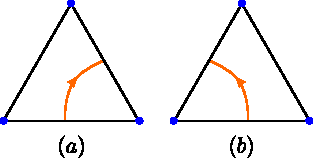
\includegraphics[width=2.1in]{figures/mono-3-crop.pdf}
\caption{右转与左转，由简单的矩阵给出。}\label{fig:mono-3}
\end{minipage}\hspace{0.4cm}
\begin{minipage}[b]{0.45\linewidth}
\centering 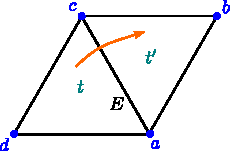
\includegraphics[width=1.6in]{figures/mono-2-crop.pdf}
\caption{穿过三角形 $t$ 与 $t'$ 之间的边 $E$。}\label{fig:mono-2}
\end{minipage}
\end{figure}

现在，$s_i,s_j,s_k$ 起初只定义在顶点 $i,j,k$ 的割缝邻域中。我们可以把它们延拓得在整个三角形 $t$ 上单值；而且事实上还能继续延拓到路径 $P$ 接下来所遇的三角形 $t'$ 中，使它们在更大的区域 $t\cup t'$ 上有定义且单值；如此继续，只要该区域保持单连通即可。我们将通过计算路径 $P$ 沿途从一组这样的基到另一组的变换，来算出单值矩阵。所需的基变换有两类。若路径经由一条边 $E$ 进入三角形 $t$、又经由边 $E'$ 离开三角形 $t$，我们就需要矩阵 $M_E^{E'}(t)$，它给出三角形 $t$ 内与两条边相联系的两组基之间的基变换，如图 85 所示% TODO 合稿改 \ref{fig:mono-3}
。另一方面，若路径经由一条边 $E$ 从三角形 $t$ 穿到三角形 $t'$，我们就需要两组不同基之间的变换 $M_t^{t'}(E)$，如图 86 所示% TODO 合稿改 \ref{fig:mono-2}
。

我们先说明如何计算 $M_E^{E'}(t)$。在三角形 $t$ 内有简单的关系
\begin{equation}
s_1 (s_2 \wedge s_3) + s_2 (s_3 \wedge s_1)+ s_3 (s_1 \wedge s_2)=0
\end{equation}
利用这一关系，基变换
\begin{equation}
\CB(E,t) = \CB(E',t) M_{E}^{E'}(t)
\end{equation}
便可轻易算出，其中
\begin{equation}\label{eq:left-right-turn}
M_{E}^{E'}(t) = \begin{cases} \begin{pmatrix} 0 & -1 \\ 1 & -1 \end{pmatrix}&
\langle E,E'\rangle = +1 \\ \begin{pmatrix} -1 & 1 \\ -1 & 0 \end{pmatrix}&
\langle E,E'\rangle = -1 \end{cases}
\end{equation}
注意 $\det M_{E}^{E'}(t)=1$，并且 $\langle E,E'\rangle=1$ 的情形对应于\emph{右}转，即图 85 中标为 a) 的那一种% TODO 合稿改 \ref{fig:mono-3}
。还要注意：右转矩阵是左转矩阵的逆。

另一方面，若 $t\cup t'$ 拼成一个四边形 $Q_E$，其顶点按逆时针顺序为 $a,b,c,d$（于是 $t$ 的顶点为 $acd$、$t'$ 的顶点为 $abc$，而 $E$ 就是边 $ac$，如图 86 所示% TODO 合稿改 \ref{fig:mono-2}
），则
\begin{equation}
\CB(E,t') = \CB(E,t)\begin{pmatrix} 0 & \frac{s_b \wedge s_c}{s_c \wedge
s_d} \\ \frac{s_a \wedge s_b}{s_d \wedge s_a} & 0 \end{pmatrix}
\end{equation}
从而
\begin{equation}\label{eq:M-edge-matrix}
M_{t}^{t'}(E) =\frac{s_b \wedge s_c}{s_c \wedge s_d} \begin{pmatrix}
0 & 1 \\ - \CX_E^T & 0 \end{pmatrix}
\end{equation}
在下文的论证中，把上式记作
\begin{equation}
\hat M_{t}^{t'}(E) :=
\begin{pmatrix} 0 & 1 \\ - \CX_E^T & 0 \end{pmatrix}
\end{equation}
会很方便。注意 $\det \hat M_{t}^{t'}(E) = \CX_E^T$。

\insfig{3.8in}{mono-1}{我们沿橙色路径、通过在相继各三角形内部及其之间的逐次基变换，来计算单值（矩阵）。}

现在考虑如图 87 那样穿过若干三角形的一条路径% TODO 合稿改 \ref{fig:mono-1}
。把基 $\CB(E_1,t_1)$ 沿一条开路平行移动，所得基 $\tilde\CB(E_1,t_1)$ 在该开路所经各相继三角形拼成的单连通区域上处处单值；于是在该开路的末三角形 $t_f$ 中有如下关系：
\begin{equation}
\CB(E_f, t_f) =\tilde\CB(E_1,t_1) M_{E_1}^{E_2}(t_1)
M_{t_1}^{t_2}(E_2) M_{E_2}^{E_3}(t_2) \cdots M_{t_{f-1}}^{t_f}(E_f)
\end{equation}
现在设路径闭合，即取 $t_f=t_1$、$E_f = E_1$。此时 $\tilde\CB(E_1,t_1) = \CB(E_1,t_1) \cdot \CU(P)$，其中 $\CU(P)$ 是闭路径 $P$ 的单值矩阵在基 $\CB(E_1,t_1)$ 下的表示。由于该基只在相差标度的意义下确定，而 $\CU(P)$ 在任何基变换下只作共轭，可见 $\CU(P)$ 是一个确定的 $SL(2,\IC)$ 矩阵，它与为构造 $\CB(E_1,t_1)$ 而对 $s_i,s_j,s_k$ 所作的标度选取无关。因此 $\CU^{-1}$ 就是上述那些 $M$-矩阵的乘积。然而，由于方程 \eqref{eq:M-edge-matrix} 中的标量前因子 $\frac{s_b \wedge s_c}{s_c \wedge s_d}$，单值矩阵 $\CU(P)$ 能否用边坐标表出，并不显然。不过我们可以用下面这个技巧。矩阵 $\CU(P)^{-1}$ 在相差一个标量因子的意义下，与把各因子 $M_{t}^{t'}(E)$ 换成 $\hat M_{t}^{t'}(E)$ 之后所得的乘积相同。也就是说，有
\begin{equation}
\CU(P)^{-1} = \kappa M_{E_1}^{E_2}(t_1) \hat M_{t_1}^{t_2}(E_2)
M_{E_2}^{E_3}(t_2) \cdots \hat M_{t_{f-1}}^{t_f}(E_f)
\end{equation}
其中 $\kappa$ 是某个标量因子。取行列式即可定出 $\kappa^2$：
\begin{equation}
\kappa^{-2}  =   \CX_{E_2}^T \cdots \CX_{E_f}^T
\end{equation}
于是 $\kappa$ 含有沿路径 $P$ 所遇各边之 $\CX_E^T$ 连乘积的平方根。为定义这个平方根，我们可以援引某种非阿贝尔版本的斯托克斯定理：若 $C$ 是带穿刺点的 $\IC\IP^1$，则闭曲线 $P$ 围出一块区域 $\CR$；而由第 5.2 节所述结果% TODO 合稿改 \ref{sec:monodromies}
的推广，有
\begin{equation}
  \CX_{E_2}^T \cdots \CX_{E_f}^T \prod_{E\in {\rm
Int}(\CR)} (\CX_E^T)^2 = \prod_{v\in {\rm Int}(\CR)} (\mu_v)^2.
\end{equation}
这个公式使我们能以典范的方式选取平方根，即
\begin{equation}
\kappa = (  \CX_{E_2}^T \cdots \CX_{E_f}^T)^{-1/2} =
\frac{\prod_{E\in {\rm Int}(\CR)} \CX_E^T}{\prod_{v\in {\rm
Int}(\CR)} \mu_v}.
\end{equation}

最后我们作几点评论：

\begin{enumerate}

\item 在上面的讨论中，我们假定了所有三角形都非退化。如果出现如图 19 那样的退化构形% TODO 合稿改 \ref{fig:degenerate-face}
，我们就把边 $E$ 视为加倍的。于是，在中心顶点处取装饰 $s_1$、在外侧顶点处取装饰 $s_2$，并在上述构造中使用三个截面 $s_1,Ms_2,s_2$，其中 $M$ 是绕中心顶点的顺时针单值（变换）。特别地，我们把 $E$ 看成具有「两侧」：左侧的基为 $\CB_{\rm left} = \{ s_1 (M s_2 \wedge s_2), M s_2 ( s_2 \wedge s_1) \}$，右侧的基为 $\CB_{\rm right} = \{ s_2 (s_1 \wedge M s_2),s_1 (M s_2 \wedge s_2) \}$。对于绕着边 $E$ 而行的路径，我们用边到边的变换把这两组基联系起来。对于从左穿到右、经过边 $E$ 的路径，我们用 $M^{-1}$ 把 $\CB_{\rm left}$ 沿该边解析延拓，得到如下基变换：
\begin{equation}
\CB_{\rm right} = \tilde \CB_{\rm left} \begin{pmatrix} 0 & \mu \\ -
\mu^{-1} & 0 \end{pmatrix}.
\end{equation}
对图 20 中那个外侧的退化三角形，也有类似的说明% TODO 合稿改 \ref{fig:degenerate-quadrilateral}
。

\item 要把这一结果推广到 $C$ 为亏格更高的带穿刺点曲面的情形，我们需要选定一组平方根 $(\CX_{E_2}^T \cdots \CX_{E_f}^T)^{-1/2}$。只需对非边界闭链的一组基给出这些平方根即可；因此，这样一组选取的全体构成 $H_1(\bar C, \IZ_2)$ 的一个挠子。

\item 单值矩阵的矩阵元显然是 $\CX_{E}^T$ 的\emph{多项式}（再除以若干 $\mu_v$ 因子）；特别地，闭路径 $P$ 的单值矩阵之迹可以写成
\begin{equation}\label{eq:UV-IR-monodromy}
{\Tr}\ \CU(P) = \sum_\gamma a_\gamma(P) \CX_\gamma.
\end{equation}
几何系数 $a_\gamma(P)$ 依赖于三角剖分，因而特别地依赖于 $\vartheta$。注意 \eqref{eq:UV-IR-monodromy} 的左端与 $\vartheta$ 无关，所以 $a_{\gamma}(P)$ 与 $\CX_\gamma^\vartheta$ 的间断必须互相抵消。在五维 Yang--Mills 理论中，${\Tr}\ \CU(P)$ 是沿 $C$ 中路径 $P$ 的、关于 $\CA$ 的超对称 Wilson 线算符的真空期望值。显然，它源自非阿贝尔六维 $(2,0)$ 理论中的一个面算符，该面算符缠绕 $C$ 中某个一维闭链与 $S^1_R$ 的乘积。这表示紫外四维规范理论中的一个线算符。视闭链 $\gamma$ 的不同，这个线算符可以是四维规范场的 Wilson 圈算符、一个 't Hooft 算符，或更一般的 Wilson--'t Hooft 算符。有鉴于此，我们把方程 \eqref{eq:UV-IR-monodromy} 解读为如下关系：它把紫外理论中定义的线算符，与这一线算符在另一组线算符基下的分解联系起来，而后者携带红外阿贝尔理论的量子数。的确，$\CX_{\gamma}$ 就是绕 $S^1_R$ 缠绕的线算符的期望值，这些线算符定义在红外的四维 $\CN=2$ 理论中（等价地说，是红外阿贝尔 $(2,0)$ 理论在 $\IR^{1,2} \times S^1_R\times \Sigma$ 上的面算符）。

存在一个依赖于 $\zeta$ 的幂零超对称算符 $Q_\zeta$，它湮灭这些算符；因此它们是超对称 't Hooft--Wilson 线算符的类似物，与 \cite{Maldacena:1998im,Rey:1998ik,geom-lang-n4} 中所讨论的那些相仿。按此解释，方程 \eqref{eq:UV-IR-monodromy} 编码了一些有趣的物理，我们希望另文讨论。

\item 关于 $SL(2,\IC)$ 联络的模空间与 $PSL(2,\IC)$ 联络的模空间之间的区别，有一点微妙之处需要说明。本文考虑的是 $C$ 上平凡化的 $SL(2,\IC)$ 主丛上的联络，或它在对中心取商后所得的平凡化 $PSL(2,\IC)$ 丛上的联络。这两种丛上的联络之间存在一一对应。然而，存在一些 $PSL(2,\IC)$ 规范变换不能提升为 $SL(2,\IC)$ 规范变换，因此 $SL(2,\IC)$ 联络的模空间是 $PSL(2,\IC)$ 联络的模空间的一个离散覆盖。$\CX_{\gamma}$ 定义在 $PSL(2,\IC)$ 联络的商模空间上，并可拉回到 $SL(2,\IC)$ 联络的模空间上。如果我们认为模空间是由单值本征值 $\mu_i$ 的指定（而不只是 $\mu_i^2$ 的指定）所确定的，那么当 $C = \IC \IP^1$ 时，$\CX_E^T$ 就唯一地确定了一个模 $SL(2,\IC)$ 规范不变的平坦 $SL(2,\IC)$ 联络。对于亏格更高的 $C$，即便指定了 $\mu_i$，$\CX_E^T$ 也不足以完全分辨 $SL(2,\IC)$ 联络模空间上的点：要由 $\CX_E^T$ 确定联络，我们还需要指定那组平方根 $(\CX_{E_2}^T \cdots \CX_{E_f}^T)^{-1/2}$。这些选取的存在引出一个问题：$\IR^3 \times S^1$ 上四维规范理论「正确」的模空间究竟是什么？它应当是 $SL(2,\IC)$ 联络的模空间、$PSL(2,\IC)$ 联络的模空间，还是 $PSL(2,\IC)$ 联络模空间的某个中间覆盖？有趣的是，定义相应的四维规范理论本身也涉及一个离散选取，而它也许正对应于上述含混之处。如 \cite{Gaiotto:2009we} 所述，相应的四维规范理论是若干 $SU(2)$ 规范群构成的广义箭图。规范群中心的一个子群 $\CC$ 在物质场上平凡地作用，于是我们有权把规范群对 $\CC$ 的任一子群取商。与众所周知的 $\CN=2^*$ $SU(2)$ 规范理论（它联系于带一个穿刺点的环面上的 Hitchin 方程）作比较，应当足以建立完整的对应词典；但我们不在此深究此事。

\end{enumerate}

\begin{yizhu}
原文在 (A.14) 处写 $\CX_\gamma$（不带任何上标），而同一段后文又写成 $\CX_\gamma^\vartheta$；按第 7 节% TODO 合稿改 \ref{sec:darboux-coordinates}
的定义，前者即后者。译文两处均照抄原文记号，未作统一。
\end{yizhu}

% =====================================================================
%  GMN2 附录 B  计算哈密顿流（Computing the Hamiltonian flows）
%  原文：wkb-paper.tex 9525–9671 行；BRIEF 印刷页 169–171（ch19 块，整块 28 式）；编号公式 (B.1)–(B.17) 共 17 条
%  块内公式全在本文件，\eqref 可用；跨块引用（(4.10)、第 5.4 节）硬编码原文编号并加 % TODO
% =====================================================================

\section{计算哈密顿流}
\label{app:poorman}

我们先作一个辅助计算。取一条路径 $\gamma$，参数化为 $z(t)$，$0\le t\le 1$；令 $z_i=z(0)$、$z_j=z(1)$。眼下先把这两点都取作正则点。设 $s_i$ 与 $s_j$ 是沿 $\gamma$ 的两个平坦截面，其边界条件固定为 $s_i(t=0)=d_i$ 与 $s_j(t=1)=d_j$。给定这两个截面，就可以考虑 $\wedge^2(V)$ 的截面 $s_i\wedge s_j$。为方便起见，我们再取 $\wedge^2(V^*)$ 的一个平坦截面 $\eps$（体积形式）；这总是做得到的，因为 $\CA$ 取值于 $sl(2)$。若用 $\eps$ 作缩并来归一化，就可以把 $s_i\wedge s_j$ 看成一个数，以下我们正是这样做的；在 $V$ 的一个局部标架中，
\begin{equation}
s_i \wedge s_j = \eps_{ab} s_i^a(t) s_j^b(t).
\end{equation}
既然 $\eps$ 与 $s_{i,j}$ 都是平坦的，$s_i\wedge s_j$ 就与 $t$ 无关。下文还便于用 $\eps$ 把 $V$ 的截面 $s_i^a$ 与 $V^*$ 的对偶截面 $s_{ia}$ 联系起来。在局部标架中，
\begin{equation}
s_{ia}(t) = \eps_{ab} s_i^b(t).
\end{equation}

现在在「所有规范场」构成的空间 $\CN$ 上定义一个函数：
\begin{equation}
\CO_{\gamma, d_i, d_j}:= \log( s_i \wedge s_j ).
\end{equation}
我们要计算 $\{\CO_{\gamma,d_i,d_j},\CA^a_{\lambda b}(z)\}$。对于与 (4.10) 相应的泊松括号，我们把它的符号取定为% TODO 合稿改 \eqref{eq:symplectic}
\begin{equation} \label{eq:spoisson}
\{ \CO ,  \CA^a_{\lambda b}(z) \} = \eps_{\lambda\mu}
\frac{\delta \CO}{\delta \CA^b_{\mu a}(z)}.
\end{equation}
取某个 $t_*$ 使 $z(t_*)\neq z$，并在该点计算 $\CO_{\gamma,d_i,d_j}$；于是 \eqref{eq:spoisson} 化为
\begin{equation}
\{\CO_{\gamma, d_i, d_j}, \CA^a_{\lambda b}(z) \}=
\frac{\eps_{\lambda\mu} }{s_i\wedge s_j} \eps_{a'b'}\left(
\frac{\delta s_i^{a'}(t_*)}{\delta \CA^b_{\mu a}(z) } s_j^{b'}(t_*)
+ s_i^{a'}(t_*) \frac{\delta s_j^{b'}(t_*)}{\delta \CA^b_{\mu a}(z) } \right).
\end{equation}
为计算它，先对平行移动引入一点记号：记 $\CA(t) = \CA_\mu(t) \dot z^\mu(t)$，并令 $U(t_1, t_2)$ 为从 $t_2$ 到 $t_1$ 的平行移动矩阵，它满足
\begin{align}
\frac{d}{dt_1} U(t_1,t_2) &= - \CA(t_1) U(t_1,t_2), \\
\frac{d}{dt_2} U(t_1,t_2) &= U(t_1,t_2) \CA(t_2),
\end{align}
以及边界条件 $U(t,t)=\mathrm{id}$。于是有
\begin{equation}
\frac{\delta}{\delta \CA^a_{\mu b}(z)} U(t_1,t_2)^c_{~d} =
\int_{t_1}^{t_2} dt\, \delta^{(2)}(z-z(t)) \dot z^\mu(t)
U(t_1,t)^c_{~a} U(t,t_2)^b_{~d}.
\end{equation}
由此可见，$s_{i,j}$ 关于 $\CA$ 的变分由下式给出：
\begin{align}
 \frac{\delta s_i^{a'}(t_*)}{\delta \CA^b_{\mu a}(z) } &= - \int_0^{t_*} dt\,
\delta^{(2)}(z-z(t)) \dot z^\mu(t) \left[ U(t_*,t)^{a'}_{~b}
s_i^a(t)- \half \delta^{a}_{~b} s_i^{a'}(t_*) \right], \\
 \frac{\delta s_j^{b'}(t_*)}{\delta \CA^b_{\mu a}(z) } &= \int_{t_*}^1 dt\,
\delta^{(2)}(z-z(t)) \dot z^\mu(t) \left[ U(t_*,t)^{b'}_{~b}
s_j^a(t)-\half \delta^{a}_{~b} s_j^{b'}(t_*) \right].
\end{align}
（出现这个减去项，是因为我们在 $sl(2)$ 联络的空间内、而不是在 $gl(2)$ 联络的空间内变分 $\CA$，所以应当把迹投影掉。）现在利用
\begin{equation}
\label{eq:rrrng}
 s_i^a(t) s_{jb}(t) - \half \delta^{a}_{~b} s_i \wedge s_j = \half
 (s_{ib} s^a_{j} + s_{jb} s_i^a )(t)
\end{equation}
（把对偶指标与基 $s_i^a$、$s_j^a$ 缩并即可证明），我们得到
\begin{equation}\label{eq:poormandeltaA}
\{\CO_{\gamma, d_i, d_j}, \CA^a_{\lambda b}(z) \} =  \half
\eps_{\lambda\mu}
 \int_{0}^1 dt\, \delta^{(2)}(z-z(t)) \dot z^\mu(t)  M(s_i,s_j)^a_{~b}(t),
\end{equation}
其中定义了算子
\begin{equation}
M(s_i,s_j)^a_{~b}(t) := \frac{s_{ib}(t) s^a_{j}(t) + s_{jb}(t)
s_i^a(t) }{s_i\wedge s_j}.
\end{equation}

现在考虑两条路径。第一条 $z_1(t)\in \gamma_1$ 是从 $z_i$ 到 $z_j$ 的路径，即我们上面一直考虑的那种。第二条 $z_2(t) \in \gamma_2$ 与 $\gamma_1$ 横截相交（或者根本不相交）。再考虑一个沿 $\gamma_2$ 平行移动的矢量 $v^a(t)$，其初始边界条件固定。我们要计算 $\{\CO_{\gamma_1, d_i, d_j}, v^a(t_*)\}$，它由下式给出：
\begin{equation}
\{ \CO_{\gamma_1, d_i, d_j}, v^a(t_*) \} = - \int_0^{t_*} dt \, \tilde U^{a}_{~b}(t_*, t)
\{\CO_{\gamma_1, d_i, d_j}, \CA(t)^{b}_{~c} \} v^c(t),
\end{equation}
其中 $\tilde U$ 是沿 $\gamma_2$ 的平行移动。利用 \eqref{eq:poormandeltaA} 可得
\begin{multline}
\{ \CO_{\gamma_1, d_i, d_j}, v^a(t_*) \} =  \\
\half \int_0^1 dt_1 \int_0^{t_*} dt_2\,
\delta^{(2)}(z_2(t_2)-z_1(t_1))\eps_{\lambda\mu} \dot
z_2^\lambda(t_2) \dot z_1^\mu(t_1) \tilde{U}^a_{~b}(t_*,t_2)
M(s_i,s_j)^{b}_{~c}(t_1) v^c(t_2).
\end{multline}
现在注意
\begin{equation}
\delta^{(2)}(z_2(t_2)-z_1(t_1))\eps_{\lambda\mu} \dot
z_2^\lambda(t_2) \dot z_1^\mu(t_1)  = -(\gamma_1\cap
\gamma_2)\delta(t_1-t_1^{int}) \delta(t_2-t_2^{int})
\end{equation}
其中 $t_i^{int}$ 是两曲线相交处的 $t$ 值，$\cap$ 表示带定向的相交数。于是得到
\begin{equation} \label{eq:flow-single}
\{ \CO_{\gamma_1, d_i, d_j}, v(t_*) \} =  \half (\gamma_1 \cap
\gamma_2) \left( \frac{s_i \wedge v}{s_i \wedge s_j}(t_2^{int})
s_j(t_*) + \frac{s_j \wedge v}{s_i \wedge s_j}(t_2^{int}) s_i(t_*)
\right) \theta(t_* - t_2^{int}).
\end{equation}
其中 $s_i$、$s_j$ 已沿 $\gamma_2$ 从交点平行移动到 $t_*$。

本附录的目标是描述由函数 $\log \CX^T_E$ 在 $\CM$ 上生成的流。要把它提升到 $\CN$ 上，需要把四个函数 $\CO_{\gamma, d_i, d_j}$ 组合起来：依次把 $\gamma$ 与四边形 $Q_E$ 的四条边等同起来，并取 $d_i$、$d_j$ 与我们在各顶点处所作的装饰选择一致。把这四条边的 \eqref{eq:flow-single} 合起来，就得到我们在第 5.4 节中所描述的那个流。% TODO 合稿改 \ref{sec:ham-flows}

严格说来，我们其实必须作正则化：把四边形稍稍形变，将其顶点从奇点处挪开，然后取顶点趋于奇点的极限。正则化后的函数 $\CO_{\gamma, d_i, d_j}$ 不是规范不变的（因为 $d_{i,j}$ 不是），但它们的组合在极限下确实变成规范不变的：回想一下，规范群 $\CG$ 只包含那些在奇点处被限制到极大环面 $\IC^\times \subset SL(2,\IC)$ 的变换；这个群把 $d_{i,j}$ 保持到整体重标度，而当我们对四条边求和时，这个整体重标度就抵消了。

% =====================================================================
%  GMN2 附录 C  WKB 误差分析（WKB error analysis）
%  原文：wkb-paper.tex 9673–9757 行；BRIEF 印刷页 169–171（ch19 块，整块 28 式）；编号公式 (C.1)–(C.11) 共 11 条，另有脚注 1 条
%  本块引用全在本文件内，\eqref 可直接用；\Pexp→\operatorname{Pexp}、\id→\mathrm{id}（preamble 未定义）
% =====================================================================

\section{WKB 误差分析}
\label{app:wkb-error}

本附录考虑指数式增长的平坦截面沿 WKB 曲线的传播。我们想看清的是：这种传播在 $\zeta\to0$ 时的渐近行为，恰好就是把 Higgs 场 $\varphi$ 的本征值 $\lambda$ 积分出来所得的结果。

更精确地说：取一个使 $\varphi$ 对角化的规范，
\begin{equation}
\varphi = \begin{pmatrix} \lambda & 0 \\ 0 & -\lambda \end{pmatrix}.
\end{equation}
然后令 $z(t)$ 是一条相位为 $\vartheta$ 的 WKB 曲线，并取 $\zeta\in\IH_\vartheta$，使得 $\re\lambda_z z'(t)/\zeta<0$。设 $s$ 是一个平坦截面，满足
\begin{equation}
s(z(0)) = \begin{pmatrix} 1 \\ 0 \end{pmatrix}.
\end{equation}
WKB 近似的命题是：当 $\zeta\to0$ 时
\begin{equation} \label{eq:wkb}
s(z(t)) \sim c(t) \begin{pmatrix} e^{-\frac{R}{\zeta} \int_{z(0)}^{z(t)} \lambda} \\ 0 \end{pmatrix},
\end{equation}
其中 $c(t)$ 是某个与 $\zeta$ 无关的函数。

为证明 \eqref{eq:wkb}，先如下定义 WKB 余项 $\psi$：
\begin{equation} \label{eq:wkb-remainder}
\psi(z) = s(z) \exp\left( \frac{R}{\zeta} \int_{z(0)}^z \lambda \right).
\end{equation}
平坦性方程 $(d+\CA)s=0$ 于是变成
\begin{align}
(\partial_{\bar z} + A_{\bar z} + R\zeta \bar\varphi_{\bar z}) \psi &= 0, \\
(\partial_z + A_z + \frac{R}{\zeta} (\varphi_z - \lambda_z\, \mathrm{id})) \psi &= 0.
\end{align}
所以沿曲线 $z(t)$，$\psi$ 的演化是
\begin{equation} \label{eq:reduced-ode}
\left( \frac{d}{dt} + B(t) \right) \psi(z(t)) = 0
\end{equation}
其中
\begin{equation}
B(t) = \frac{R}{\zeta} z' \begin{pmatrix} 0 & 0 \\ 0 & -2\lambda_z \end{pmatrix} + z' A_z + \bar z' (A_{\bar z} + R\zeta \bar\varphi_{\bar z}).
\end{equation}

所要的 \eqref{eq:wkb} 等价于说：$\lim_{\zeta\to0}\psi$ 存在，而且其第二个分量消失。为什么应当如此？直觉是：$B(t)$ 中当 $\zeta\to0$ 时不为有限的项，只有右下角那一项 $-2Rz'\lambda_z/\zeta$；而这一项的唯一效果，是在 $\psi$ 的第二个分量中引入一个形如 $e^{-\#/\zeta}$ 的因子（其中 $\re\# > 0$），于是该分量在 $\zeta\to0$ 时消失。

为论证这一直觉，令 $B_0(t)=g(t)B(t)g^{-1}(t)$ 是 $B(t)$ 的对角化。我们希望证明
\begin{equation} \label{eq:wkb-interm}
\lim_{\zeta\to0} \bigg\lVert \operatorname{Pexp}\int_0^t B(t) - \operatorname{Pexp}\int_0^t B_0(t) \bigg\rVert = 0.
\end{equation}
一旦确立了 \eqref{eq:wkb-interm}，就可以在 $\zeta\to0$ 极限下用 $B_0$ 代替 $B$ 来计算 $\psi$ 的平行移动；那便证明了所要的 \eqref{eq:wkb}。

一个直接的计算——只用到一个事实：$B(t)$ 是 $2\times2$ 矩阵，其右下角元素的实部趋于 $-\infty$，而其余元素都保持有限——表明 $\exp B_0(t)$ 在 $\zeta\to0$ 时有界，并且可以选取 $g(t)$ 使 $g(t)\to\mathrm{id}$（当 $\zeta\to0$ 时）。由这两件事即得 \eqref{eq:wkb-interm}。为看清这一点，我们先把区间切成小段，使 $B$ 在每段上缓变，从而归结为 $B$ 与 $t$ 无关的情形。此时 \eqref{eq:wkb-interm} 化为
\begin{equation}
\lim_{\zeta\to0} \lVert e^{tB} - e^{tB_0} \rVert = 0.
\end{equation}
而这又可由 $B=gB_0g^{-1}$、$\lim_{\zeta\to0}g=\mathrm{id}$ 以及 $\lim_{\zeta\to0}e^{tB_0}$ 的存在性推出。\footnote{正是在这里，我们用到了如下事实：当 $\zeta\to0$ 时，$B(t)$ 右下角元素的实部趋于 $-\infty$，而非 $+\infty$。} 这就完成了 \eqref{eq:wkb-interm} 从而 \eqref{eq:wkb} 的证明。

更精确地说，我们是在 WKB 曲线始于正则点的情形下证明 \eqref{eq:wkb} 的。而我们的应用需要考虑 WKB 曲线始于奇点的情形，不妨设该奇点位于 $z(0)$。这时显然不能指望 \eqref{eq:wkb} 原封不动地成立，因为 $\int_{z(0)}^{z(t)}\lambda$ 发散。替代的办法是另取一个函数 $I(z)$，它定义在 WKB 曲线的一个邻域上（奇点除外），满足 $dI=\lambda$。于是与上面类似的论证表明，存在一个平坦截面 $s$，它在 $\zeta\to0$ 时的行为是
\begin{equation} \label{eq:wkb-sing}
s(z(t)) \sim \begin{pmatrix} c(t) e^{-\frac{R}{\zeta} I(z(t))} \\ 0 \end{pmatrix}.
\end{equation}
而且可以取 $s$ 为与 WKB 曲线 $z(t)$ 及奇点 $z(0)$ 相伴的那个小平坦截面。

% =====================================================================
%  GMN2 附录 D  多中心 Taub-NUT 上的全纯坐标（Holomorphic coordinates on multi-center Taub-NUT）
%  原文：wkb-paper.tex 9760–9870 行；印刷页 p.172–174；编号公式 (D.1)–(D.15) 共 15 条
%  脚注 0 条；插图 0 幅
%  main.tex 第 67 行 \appendix 生效时，本节自动编号为 D，公式随之为 (D.1)…，与原文一致
%  块内引用（\eqref{eq:holoTN1}）直接用；跨块引用（第 3.2 节、第 3.2.5 节）硬编码原文编号并加 % TODO
%  原文末条 align 的两行 (D.14)(D.15) 按规范拆成两条 equation
% =====================================================================

\section{多中心 Taub-NUT 上的全纯坐标}\label{app:HoloTN}

我们从 Gibbons--Hawking 拟设开始。Taub-NUT 空间 $TN$ 带有一个映射 $\pi: TN \to \IR^3$，其一般纤维是一个圆，度量为
\begin{equation}
ds^2 = V^{-1} \Theta^2 + V (d\vec r)^2,
\end{equation}
其中 $d \Theta = \pi^*( *dV)$。整体良定义的一形式 $\Theta$ 由 $\pi_* \Theta = 4\pi$ 归一。

Taub-NUT 的中心位于 $\vec r_a$，而
\begin{equation}
V = 1 + \sum_a \frac{1}{\vert \vec r - \vec r_a \vert}.
\end{equation}
令 $z=x^1 + i x^2$。某个复结构下的全纯函数被
\begin{equation}
\p_{\bar z} - \Theta_{\bar z} \p_\psi
\end{equation}
\begin{equation}
\p_3 + (i V - \Theta_3) \p_\psi
\end{equation}
所湮灭，其中 $\p_\psi$ 是整体良定义的矢量场，它生成纤维内的旋转，并归一为 $\langle \Theta, \p_\psi \rangle = 1$。

为写出全纯坐标，用片覆盖流形比较方便。对每个中心引入角坐标 $(\theta_a, \phi_a)$。我们将定义片 $\CU_\epsilon$，其中 $\epsilon$ 是一个矢量，对每个中心各有一个分量，且 $\epsilon_a = \pm 1$。我们令 $\CU_\epsilon$ 为使 $\theta_a \not= \half(1-\epsilon_a)\pi$ 的那些 $\vec r$（$\vec r\not=\vec r_a$）的集合。在每个片上，都可以定义周期为 $4\pi$ 的纤维坐标 $\psi_\epsilon$，使得
\begin{equation}
\Theta = d \psi_\epsilon + A_\epsilon
\end{equation}
\begin{equation}
A_\epsilon = \sum_a \epsilon_a (1 + \epsilon_a\cos\theta_a) d \phi_a
\end{equation}
由于 $\Theta$ 整体良定义，由此可以读出 $\psi_\epsilon$ 的过渡函数。现在，定义下面这个量比较方便：
\begin{equation}
R_{a,\pm}: = \vert \vec r - \vec r_a\vert \pm (x_3 - x_{3,a} )
\end{equation}
注意 $R_{a,+}R_{a,-} = \vert z-z_a\vert^2$。直接验证可知
\begin{equation}\label{eq:holoTN1}
\tilde U_\epsilon = \prod_{\epsilon_a=+1} (R_{a,-})^{-1/2}
\prod_{\epsilon_a = -1} (R_{a,+})^{1/2} e^{\half (i \psi_\epsilon + x_3)}
\end{equation}
被反全纯矢量场湮灭。若把 \eqref{eq:holoTN1} 乘上 $\prod_{\epsilon_a=+1}(z-z_a)$，全纯性得以保持；我们正是这样做来定义
\begin{equation}
U_\epsilon = \prod_a (R_{a,+})^{1/2} \prod_{\epsilon_a=+1}
\frac{z-z_a}{\vert z-z_a\vert} e^{\half (i \psi_\epsilon + x_3)}
\end{equation}
可以验证 $U_\epsilon$ 实际上与 $\epsilon$ 无关，也就是说，它是\emph{整体良定义}的。正如我们已经说过的，它在 $TN$ 上是全纯的。它的除子是若干全纯圆盘的不交并，这些圆盘投影到直线 $\theta_a = \pi$ 上。今后我们略去下标 $\epsilon$，直接写作 $U$。$TN$ 上任一绕纤维的绕数为 1 的整体全纯函数，必定是 $z$ 的多项式乘以 $U$。

现在也可以验证
\begin{equation}
W = \prod_a (z-z_a)/U
\end{equation}
是整体良定义且全纯的。它的除子是若干全纯圆盘的并，这些圆盘投影到直线 $\theta_a = 0$ 上。可以显式地写出
\begin{equation}
W = \prod_a (R_{a,-})^{1/2} \prod_{\epsilon_a=-1}\frac{ z-z_a}{\vert z-z_a\vert} e^{-\half ( i \psi_\epsilon + x_3)}.
\end{equation}

在第 3.2 节% TODO 合稿改 \ref{subsec:WittenConstruction}
中，我们考虑固定 $\vec r$、令 $x_{3,a} \to \pm \infty$ 的极限。假设对 $a \in \CR$ 取 $x_{3,a} \to +\infty$，对 $a \in \CL$ 取 $x_{3,a} \to -\infty$。那么 $\vec r$ 落在这样的片里：对 $a \in \CR$ 有 $\epsilon_a = +1$，对 $a\in \CL$ 有 $\epsilon_a = -1$。可以算得
\begin{equation}
\tilde U_\epsilon \to \prod_{a\in \CR} (2 x_{3,a})^{-1/2}
\prod_{a\in \CL} (2 \vert x_{3,a}\vert)^{+1/2} e^{\half (i \psi +x_3)}
\end{equation}
因此，为使极限良好，我们在这个特殊的坐标片里把 $U$ 归一化，使得
\begin{equation}
U = \prod_{a\in \CR} (z-z_a) \prod_{a\in \CR} \left(
\frac{2x_{3,a}}{R_{a,-}} \right)^{1/2} \prod_{a \in \CL}
\left(\frac{ R_{a,+}}{2\vert x_{3,a}\vert}\right)^{1/2} e^{\half (i \psi_\epsilon + x_3)}
\end{equation}

现在，我们可以把这个结果用到第 3.2.5 节% TODO 合稿改 \ref{subsubsec:LinConfQuivMatt}
的讨论中。我们把柱坐标取为 $t = e^{-\half (i \psi_\epsilon + x_3)}$，把 $z$ 与 $v$ 等同，而把 $x^3$ 与 $x^6$ 等同。于是在极限下
\begin{equation}
U \to t^{-1} \prod_{a\in \CR} (v-v_a),
\end{equation}
\begin{equation}
W \to t \prod_{a\in \CL} (v-v_a),
\end{equation}
其中 $(t, v)$ 是 $T^*\IC^\times$ 上的自然全纯坐标。

% =====================================================================
%  GMN2 附录 E  二阶离散导数非正的整数组态（Configurations of integers with
%  nonpositive second discrete derivative）
%  原文：wkb-paper.tex 9873–9906 行；印刷页 p.174–175；编号公式 (E.1)–(E.2) 共 2 条
%  脚注 0 条；插图 3 幅：convexk-1（图 88）+ convexk-2（图 89）+ convexk-3（图 90）
%        原文是一处 \insthreefigs 并排、三个 \caption，故占三个图号；preamble 未定义该宏，
%        此处按 ch13/appA 先例展开为一个 figure + 三个 minipage，保留原三个图号
%  main.tex 第 67 行 \appendix 生效时，本节自动编号为 E，公式随之为 (E.1)…，与原文一致
%  块内引用（\eqref{eq:NegBetas2}）直接用；跨块引用（第 3.2 节、(3.42)）硬编码原文编号并加 % TODO
% =====================================================================

\section{二阶离散导数非正的整数组态}\label{app:ConvexKay}

这里我们总结一些关于整数族 $\{ k_\alpha \}$（$0 \leq \alpha \leq n+1$）的简单观察；这些整数出现在第 3.2 节% TODO 合稿改 \ref{subsec:WittenConstruction}
的 D4/NS5-膜位形中。按照 (3.42)，这些位形满足% TODO 合稿改 \eqref{eq:NegBetas}
\begin{equation} \label{eq:NegBetas2}
- 2k_\alpha + k_{\alpha+1} + k_{\alpha-1} + d_\alpha \leq 0, \qquad\qquad 1\leq \alpha \leq n.
\end{equation}
由于 $d_\alpha \geq 0$，\eqref{eq:NegBetas2} 表明：若把 $k_\alpha$ 看作 $\alpha$ 的函数，则它的二阶离散导数非正，即其图像是凸的。

\begin{figure}[htbp]
\centering
\begin{minipage}[b]{0.31\linewidth}
\centering 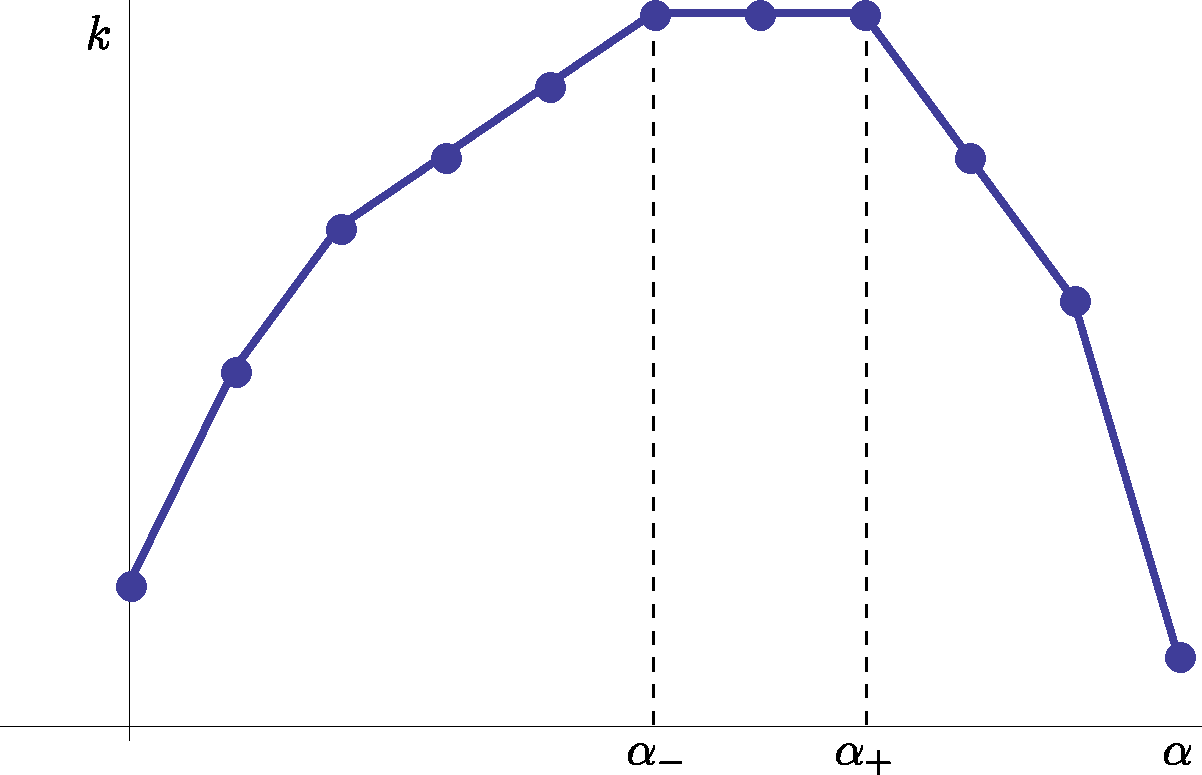
\includegraphics[width=1.15in]{figures/convexk-1-crop.pdf}
\caption{当 $k_1-k_0>0$ 时，满足 $2k_\alpha-k_{\alpha-1} - k_{\alpha+1}\geq 0$ 的一组整数 $k_\alpha$ 的典型图像。}\label{fig:convexk-1}
\end{minipage}\hspace{0.25cm}
\begin{minipage}[b]{0.31\linewidth}
\centering 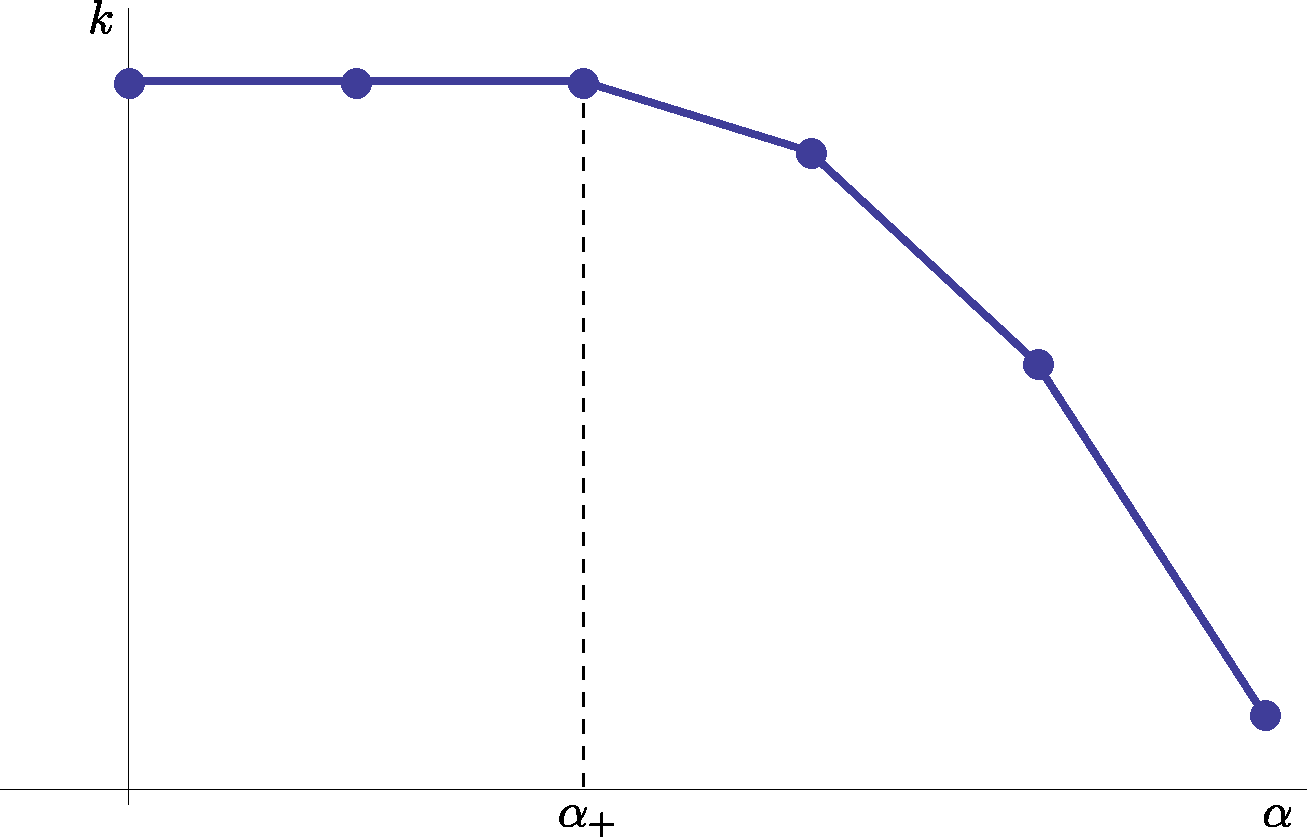
\includegraphics[width=1.15in]{figures/convexk-2-crop.pdf}
\caption{当 $k_1-k_0=0$ 时，满足 $2k_\alpha-k_{\alpha-1} - k_{\alpha+1}\geq 0$ 的一组整数 $k_\alpha$ 的典型图像。}\label{fig:convexk-2}
\end{minipage}\hspace{0.25cm}
\begin{minipage}[b]{0.31\linewidth}
\centering 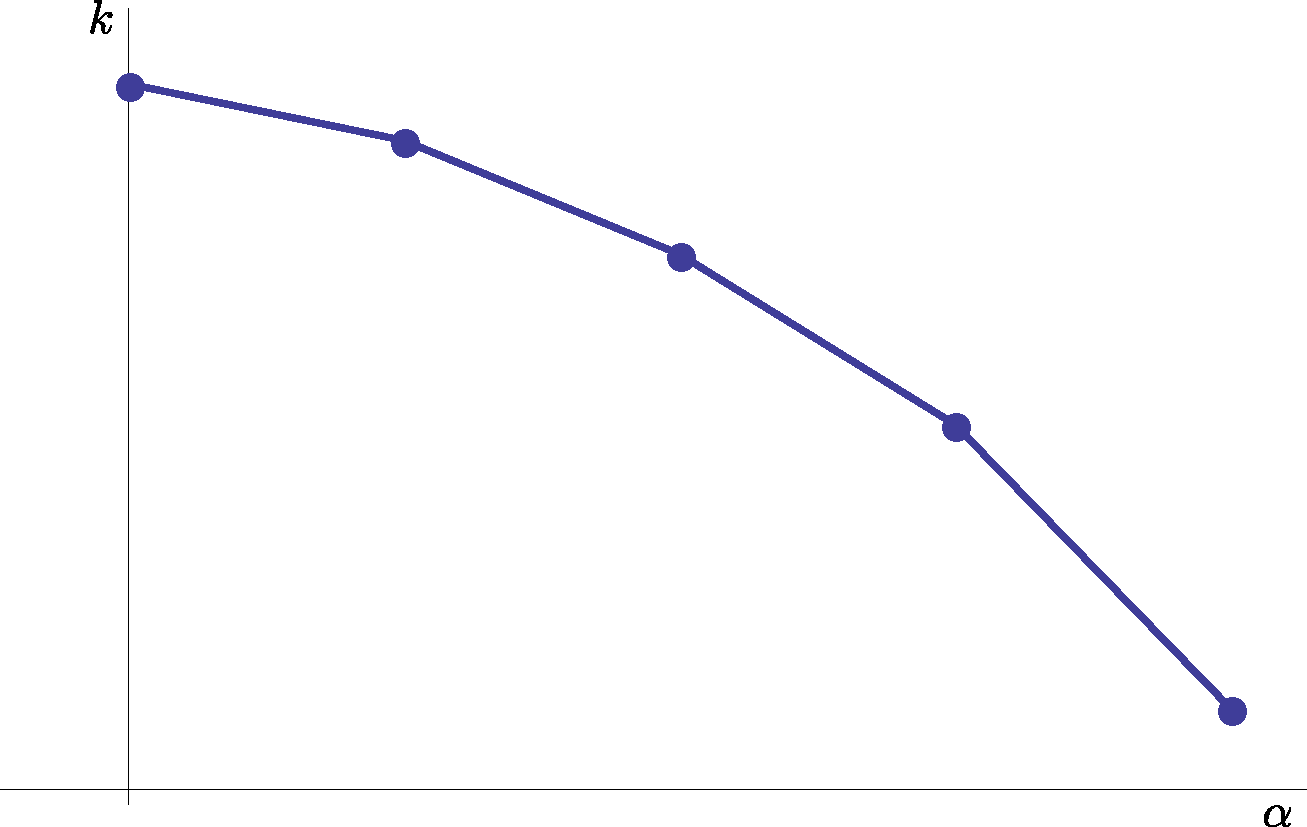
\includegraphics[width=1.15in]{figures/convexk-3-crop.pdf}
\caption{当 $k_1-k_0<0$ 时，满足 $2k_\alpha-k_{\alpha-1} - k_{\alpha+1}\geq 0$ 的一组整数 $k_\alpha$ 的典型图像。}\label{fig:convexk-3}
\end{minipage}
\end{figure}

要区分三种基本情形。第一种是 $k_1-k_0 > 0$。此时 $k_\alpha$ 在 $0\leq \alpha \leq \alpha_-$ 上严格递增，在 $\alpha_-\leq \alpha \leq \alpha_+$ 上取到最大值 $K$，并在 $\alpha \geq \alpha_+$ 上严格递减（见图 88）。% TODO 合稿改 \ref{fig:convexk-1}
若 $k_1 - k_0 = 0$，则行为类似，只是 $\alpha_- = 0$（见图 89）。% TODO 合稿改 \ref{fig:convexk-2}
最后，若 $k_1 - k_0 < 0$，则 $\alpha_- = \alpha_+ = 0$，如图 90 所示。% TODO 合稿改 \ref{fig:convexk-3}

还有一个重要的特殊情形：二阶离散导数恒为零，即对 $1 \leq \alpha \leq n$ 有 $-2k_\alpha + k_{\alpha+1} + k_{\alpha-1} = 0$。此时图像就是一条直线，亦即
\begin{equation}
k_\alpha = k_0 + \alpha r, \qquad\qquad 0 \leq \alpha \leq n+1.
\end{equation}

% ------------------------------ 参考文献 ------------------------------
% 由 0907.3987v2 的 wkb-paper.bbl 机械转换（去掉 bbl 包装，反斜杠N -> 反斜杠CN）
\begin{thebibliography}{10}

\bibitem{Gaiotto:2008cd}
D.~Gaiotto, G.~W. Moore, and A.~Neitzke, ``{Four-dimensional wall-crossing via
  three-dimensional field theory},''
\href{http://www.arXiv.org/abs/0807.4723}{{\tt 0807.4723}}.
%%CITATION = 0807.4723;%%.

\bibitem{Witten:1997sc}
E.~Witten, ``Solutions of four-dimensional field theories via {M}-theory,''
  {\em Nucl. Phys.} {\bf B500} (1997) 3--42,
\href{http://www.arXiv.org/abs/hep-th/9703166}{{\tt hep-th/9703166}}.
%%CITATION = NUPHA,B500,3;%%.

\bibitem{Klemm:1996bj}
A.~Klemm, W.~Lerche, P.~Mayr, C.~Vafa, and N.~P. Warner, ``{Self-Dual Strings
  and N=2 Supersymmetric Field Theory},'' {\em Nucl. Phys.} {\bf B477} (1996)
  746--766,
\href{http://www.arXiv.org/abs/hep-th/9604034}{{\tt hep-th/9604034}}.
%%CITATION = HEP-TH/9604034;%%.

\bibitem{irkm}
P.~Boalch, ``{I}rregular connections and {K}ac-{M}oody root systems,''
  \href{http://www.arXiv.org/abs/0806.1050}{{\tt 0806.1050}}.

\bibitem{Strominger:1996ac}
A.~Strominger, ``Open {$p$}-branes,'' {\em Phys. Lett.} {\bf B383} (1996)
  44--47,
\href{http://arXiv.org/abs/hep-th/9512059}{{\tt hep-th/9512059}}.
%%CITATION = HEP-TH 9512059;%%.

\bibitem{ks1}
M.~Kontsevich and Y.~Soibelman, ``{S}tability structures, motivic
  {D}onaldson-{T}homas invariants and cluster transformations,''
  \href{http://www.arXiv.org/abs/0811.2435}{{\tt 0811.2435}}.

\bibitem{Nekrasov:2009ui}
N.~A. Nekrasov and S.~L. Shatashvili, ``{Quantum integrability and
  supersymmetric vacua},''
\href{http://www.arXiv.org/abs/0901.4748}{{\tt 0901.4748}}.
%%CITATION = 0901.4748;%%.

\bibitem{Dorey:1999uk}
P.~Dorey and R.~Tateo, ``{On the relation between Stokes multipliers and the
  T-Q systems of conformal field theory},'' {\em Nucl. Phys.} {\bf B563} (1999)
  573--602,
\href{http://www.arXiv.org/abs/hep-th/9906219}{{\tt hep-th/9906219}}.
%%CITATION = HEP-TH/9906219;%%.

\bibitem{Dorey:1996re}
P.~Dorey and R.~Tateo, ``{Excited states by analytic continuation of TBA
  equations},'' {\em Nucl. Phys.} {\bf B482} (1996) 639--659,
\href{http://www.arXiv.org/abs/hep-th/9607167}{{\tt hep-th/9607167}}.
%%CITATION = HEP-TH/9607167;%%.

\bibitem{MR2233852}
V.~Fock and A.~Goncharov, ``Moduli spaces of local systems and higher
  {T}eichm\"uller theory,'' {\em Publ. Math. Inst. Hautes \'Etudes Sci.}
  (2006), no.~103, 1--211, \href{http://www.arXiv.org/abs/math/0311149}{{\tt
  math/0311149}}.

\bibitem{Alday:2009yn}
L.~F. Alday and J.~Maldacena, ``{Null polygonal Wilson loops and minimal
  surfaces in Anti- de-Sitter space},''
\href{http://www.arXiv.org/abs/0904.0663}{{\tt 0904.0663}}.
%%CITATION = 0904.0663;%%.

\bibitem{gmn5-to-appear}
D.~Gaiotto, G.~W. Moore, and A.~Neitzke, ``{Spectral networks}.''
\newblock In preparation.

\bibitem{gmn6-to-appear}
D.~Gaiotto, G.~W. Moore, and A.~Neitzke, ``Spin lifts and spectral networks.''
\newblock In preparation.

\bibitem{geom-lang-n4}
A.~Kapustin and E.~Witten, ``{E}lectric-magnetic duality and the geometric
  {L}anglands program,'' \href{http://www.arXiv.org/abs/hep-th/0604151}{{\tt
  hep-th/0604151}}.

\bibitem{Gaiotto:2009we}
D.~Gaiotto, ``{N=2 dualities},''
\href{http://www.arXiv.org/abs/0904.2715}{{\tt 0904.2715}}.
%%CITATION = 0904.2715;%%.

\bibitem{Cecotti:1993rm}
S.~Cecotti and C.~Vafa, ``On classification of {$\CN=2$} supersymmetric
  theories,'' {\em Commun. Math. Phys.} {\bf 158} (1993) 569--644,
\href{http://www.arXiv.org/abs/hep-th/9211097}{{\tt hep-th/9211097}}.
%%CITATION = HEP-TH 9211097;%%.

\bibitem{Denef:2007vg}
F.~Denef and G.~W. Moore, ``Split states, entropy enigmas, holes and halos,''
\href{http://www.arXiv.org/abs/hep-th/0702146}{{\tt hep-th/0702146}}.
%%CITATION = HEP-TH 0702146;%%.

\bibitem{Denef:2000nb}
F.~Denef, ``{Supergravity flows and D-brane stability},'' {\em JHEP} {\bf 08}
  (2000) 050,
\href{http://www.arXiv.org/abs/hep-th/0005049}{{\tt hep-th/0005049}}.
%%CITATION = HEP-TH/0005049;%%.

\bibitem{Witten:1995zh}
E.~Witten, ``{Some comments on string dynamics},''
\href{http://www.arXiv.org/abs/hep-th/9507121}{{\tt hep-th/9507121}}.
%%CITATION = HEP-TH/9507121;%%.

\bibitem{Witten:1995em}
E.~Witten, ``{Five-branes and M-theory on an orbifold},'' {\em Nucl. Phys.}
  {\bf B463} (1996) 383--397,
\href{http://www.arXiv.org/abs/hep-th/9512219}{{\tt hep-th/9512219}}.
%%CITATION = HEP-TH/9512219;%%.

\bibitem{Seiberg:1996vs}
N.~Seiberg and E.~Witten, ``{Comments on String Dynamics in Six Dimensions},''
  {\em Nucl. Phys.} {\bf B471} (1996) 121--134,
\href{http://www.arXiv.org/abs/hep-th/9603003}{{\tt hep-th/9603003}}.
%%CITATION = HEP-TH/9603003;%%.

\bibitem{Seiberg:1997ax}
N.~Seiberg, ``{Notes on theories with 16 supercharges},'' {\em Nucl. Phys.
  Proc. Suppl.} {\bf 67} (1998) 158--171,
\href{http://www.arXiv.org/abs/hep-th/9705117}{{\tt hep-th/9705117}}.
%%CITATION = HEP-TH/9705117;%%.

\bibitem{Seiberg:1997zk}
N.~Seiberg, ``{New theories in six dimensions and matrix description of
  M-theory on $T^5$ and $T^5 / \IZ_2$},'' {\em Phys. Lett.} {\bf B408} (1997)
  98--104,
\href{http://www.arXiv.org/abs/hep-th/9705221}{{\tt hep-th/9705221}}.
%%CITATION = HEP-TH/9705221;%%.

\bibitem{Aharony:1998an}
O.~Aharony, M.~Berkooz, and N.~Seiberg, ``Light-cone description of (2,0)
  superconformal theories in six dimensions,'' {\em Adv. Theor. Math. Phys.}
  {\bf 2} (1998) 119--153,
\href{http://www.arXiv.org/abs/hep-th/9712117}{{\tt hep-th/9712117}}.
%%CITATION = HEP-TH 9712117;%%.

\bibitem{Bhattacharya:2008zy}
J.~Bhattacharya, S.~Bhattacharyya, S.~Minwalla, and S.~Raju, ``{Indices for
  Superconformal Field Theories in 3,5 and 6 Dimensions},'' {\em JHEP} {\bf 02}
  (2008) 064,
\href{http://www.arXiv.org/abs/0801.1435}{{\tt 0801.1435}}.
%%CITATION = 0801.1435;%%.

\bibitem{Lee:2006gqa}
K.-M. Lee and H.-U. Yee, ``{BPS string webs in the 6-dim (2,0) theories},''
  {\em JHEP} {\bf 03} (2007) 057,
\href{http://www.arXiv.org/abs/hep-th/0606150}{{\tt hep-th/0606150}}.
%%CITATION = HEP-TH/0606150;%%.

\bibitem{Sen:1997xi}
A.~Sen, ``{String network},'' {\em JHEP} {\bf 03} (1998) 005,
\href{http://www.arXiv.org/abs/hep-th/9711130}{{\tt hep-th/9711130}}.
%%CITATION = HEP-TH/9711130;%%.

\bibitem{Aharony:1997bh}
O.~Aharony, A.~Hanany, and B.~Kol, ``{Webs of (p,q) 5-branes, five dimensional
  field theories and grid diagrams},'' {\em JHEP} {\bf 01} (1998) 002,
\href{http://www.arXiv.org/abs/hep-th/9710116}{{\tt hep-th/9710116}}.
%%CITATION = HEP-TH/9710116;%%.

\bibitem{Dasgupta:1997pu}
K.~Dasgupta and S.~Mukhi, ``{BPS nature of 3-string junctions},'' {\em Phys.
  Lett.} {\bf B423} (1998) 261--264,
\href{http://www.arXiv.org/abs/hep-th/9711094}{{\tt hep-th/9711094}}.
%%CITATION = HEP-TH/9711094;%%.

\bibitem{Witten:1988ze}
E.~Witten, ``{Topological Quantum Field Theory},'' {\em Commun. Math. Phys.}
  {\bf 117} (1988)
353.
%%CITATION = CMPHA,117,353;%%.

\bibitem{Brandhuber:1996xk}
A.~Brandhuber and S.~Stieberger, ``{Self-dual strings and stability of BPS
  states in N = 2 SU(2) gauge theories},'' {\em Nucl. Phys.} {\bf B488} (1997)
  199--222,
\href{http://www.arXiv.org/abs/hep-th/9610053}{{\tt hep-th/9610053}}.
%%CITATION = HEP-TH/9610053;%%.

\bibitem{Mikhailov:1997jv}
A.~Mikhailov, ``{BPS states and minimal surfaces},'' {\em Nucl. Phys.} {\bf
  B533} (1998) 243--274,
\href{http://www.arXiv.org/abs/hep-th/9708068}{{\tt hep-th/9708068}}.
%%CITATION = HEP-TH/9708068;%%.

\bibitem{MR89a:32021}
N.~J. Hitchin, ``The self-duality equations on a {R}iemann surface,'' {\em
  Proc. London Math. Soc. (3)} {\bf 55} (1987), no.~1, 59--126.

\bibitem{Cherkis:1997aa}
S.~A. Cherkis and A.~Kapustin, ``{Singular monopoles and supersymmetric gauge
  theories in three dimensions},'' {\em Nucl. Phys.} {\bf B525} (1998)
  215--234,
\href{http://www.arXiv.org/abs/hep-th/9711145}{{\tt hep-th/9711145}}.
%%CITATION = HEP-TH/9711145;%%.

\bibitem{Gukov:1998kt}
S.~Gukov and A.~Kapustin, ``{New N = 2 superconformal field theories from M/F
  theory orbifolds},'' {\em Nucl. Phys.} {\bf B545} (1999) 283--308,
\href{http://www.arXiv.org/abs/hep-th/9808175}{{\tt hep-th/9808175}}.
%%CITATION = HEP-TH/9808175;%%.

\bibitem{Kapustin:1998xn}
A.~Kapustin, ``{Solution of N = 2 gauge theories via compactification to three
  dimensions},'' {\em Nucl. Phys.} {\bf B534} (1998) 531--545,
\href{http://www.arXiv.org/abs/hep-th/9804069}{{\tt hep-th/9804069}}.
%%CITATION = HEP-TH/9804069;%%.

\bibitem{Cherkis:2000cj}
S.~A. Cherkis and A.~Kapustin, ``{Nahm transform for periodic monopoles and N =
  2 super Yang-Mills theory},'' {\em Commun. Math. Phys.} {\bf 218} (2001)
  333--371,
\href{http://www.arXiv.org/abs/hep-th/0006050}{{\tt hep-th/0006050}}.
%%CITATION = HEP-TH/0006050;%%.

\bibitem{Gorsky:1995zq}
A.~Gorsky, I.~Krichever, A.~Marshakov, A.~Mironov, and A.~Morozov,
  ``{Integrability and Seiberg-Witten exact solution},'' {\em Phys. Lett.} {\bf
  B355} (1995) 466--474,
\href{http://www.arXiv.org/abs/hep-th/9505035}{{\tt hep-th/9505035}}.
%%CITATION = HEP-TH/9505035;%%.

\bibitem{Martinec:1995by}
E.~J. Martinec and N.~P. Warner, ``{Integrable systems and supersymmetric gauge
  theory},'' {\em Nucl. Phys.} {\bf B459} (1996) 97--112,
\href{http://www.arXiv.org/abs/hep-th/9509161}{{\tt hep-th/9509161}}.
%%CITATION = HEP-TH/9509161;%%.

\bibitem{Donagi:1996cf}
R.~Y. Donagi and E.~Witten, ``Supersymmetric {Y}ang-{M}ills theory and
  integrable systems,'' {\em Nucl. Phys.} {\bf B460} (1996) 299--334,
\href{http://www.arXiv.org/abs/hep-th/9510101}{{\tt hep-th/9510101}}.
%%CITATION = HEP-TH 9510101;%%.

\bibitem{Itoyama:1995nv}
H.~Itoyama and A.~Morozov, ``{Integrability and Seiberg-Witten theory: Curves
  and periods},'' {\em Nucl.Phys.} {\bf B477} (1996) 855--877,
  \href{http://www.arXiv.org/abs/hep-th/9511126}{{\tt hep-th/9511126}}.

\bibitem{Seiberg:1996nz}
N.~Seiberg and E.~Witten, ``Gauge dynamics and compactification to three
  dimensions,''
\href{http://www.arXiv.org/abs/hep-th/9607163}{{\tt hep-th/9607163}}.
%%CITATION = HEP-TH 9607163;%%.

\bibitem{Gukov:2006jk}
S.~Gukov and E.~Witten, ``{G}auge theory, ramification, and the geometric
  {L}anglands program,''
\href{http://www.arXiv.org/abs/hep-th/0612073}{{\tt hep-th/0612073}}.
%%CITATION = HEP-TH/0612073;%%.

\bibitem{Frenkel:2007tx}
E.~Frenkel and E.~Witten, ``{Geometric Endoscopy and Mirror Symmetry},''
\href{http://www.arXiv.org/abs/0710.5939}{{\tt 0710.5939}}.
%%CITATION = 0710.5939;%%.

\bibitem{Harvey:1995tg}
J.~A. Harvey, G.~W. Moore, and A.~Strominger, ``{R}educing {S} duality to {T}
  duality,'' {\em Phys. Rev.} {\bf D52} (1995) 7161--7167,
\href{http://www.arXiv.org/abs/hep-th/9501022}{{\tt hep-th/9501022}}.
%%CITATION = HEP-TH 9501022;%%.

\bibitem{Bershadsky:1995vm}
M.~Bershadsky, A.~Johansen, V.~Sadov, and C.~Vafa, ``Topological reduction of
  4-d {SYM} to 2-d sigma models,'' {\em Nucl. Phys.} {\bf B448} (1995)
  166--186,
\href{http://arXiv.org/abs/hep-th/9501096}{{\tt hep-th/9501096}}.
%%CITATION = HEP-TH 9501096;%%.

\bibitem{Witten:2007td}
E.~Witten, ``Gauge theory and wild ramification,''
\href{http://www.arXiv.org/abs/0710.0631}{{\tt 0710.0631}}.
%%CITATION = ARXIV:0710.0631;%%.

\bibitem{Fayyazuddin:1997by}
A.~Fayyazuddin and M.~Spalinski, ``{The Seiberg-Witten differential from
  M-theory},'' {\em Nucl. Phys.} {\bf B508} (1997) 219--228,
\href{http://www.arXiv.org/abs/hep-th/9706087}{{\tt hep-th/9706087}}.
%%CITATION = HEP-TH/9706087;%%.

\bibitem{Henningson:1997hy}
M.~Henningson and P.~Yi, ``{Four-dimensional BPS-spectra via M-theory},'' {\em
  Phys. Rev.} {\bf D57} (1998) 1291--1298,
\href{http://www.arXiv.org/abs/hep-th/9707251}{{\tt hep-th/9707251}}.
%%CITATION = HEP-TH/9707251;%%.

\bibitem{Argyres:1995wt}
P.~C. Argyres, M.~R. Plesser, and A.~D. Shapere, ``{The Coulomb phase of $\CN=2$
  supersymmetric QCD},'' {\em Phys. Rev. Lett.} {\bf 75} (1995) 1699--1702,
\href{http://www.arXiv.org/abs/hep-th/9505100}{{\tt hep-th/9505100}}.
%%CITATION = HEP-TH/9505100;%%.

\bibitem{Hanany:1996ie}
A.~Hanany and E.~Witten, ``{Type IIB superstrings, BPS monopoles, and three-
  dimensional gauge dynamics},'' {\em Nucl. Phys.} {\bf B492} (1997) 152--190,
\href{http://www.arXiv.org/abs/hep-th/9611230}{{\tt hep-th/9611230}}.
%%CITATION = HEP-TH/9611230;%%.

\bibitem{Katz:1997eq}
S.~Katz, P.~Mayr, and C.~Vafa, ``{Mirror symmetry and exact solution of 4D N =
  2 gauge theories. I},'' {\em Adv. Theor. Math. Phys.} {\bf 1} (1998) 53--114,
\href{http://www.arXiv.org/abs/hep-th/9706110}{{\tt hep-th/9706110}}.
%%CITATION = HEP-TH/9706110;%%.

\bibitem{MR1206652}
H.~Konno, ``Construction of the moduli space of stable parabolic {H}iggs
  bundles on a {R}iemann surface,'' {\em J. Math. Soc. Japan} {\bf 45} (1993),
  no.~2, 253--276.

\bibitem{MR1397988}
H.~Nakajima, ``Hyper-{K}\"ahler structures on moduli spaces of parabolic
  {H}iggs bundles on {R}iemann surfaces,'' in {\em Moduli of vector bundles
  ({S}anda, 1994; {K}yoto, 1994)}, vol.~179 of {\em Lecture Notes in Pure and
  Appl. Math.}, pp.~199--208.
\newblock Dekker, New York, 1996.

\bibitem{wnh}
O.~Biquard and P.~Boalch, ``{W}ild nonabelian {H}odge theory on curves,''
  \href{http://www.arXiv.org/abs/math/0111098}{{\tt math/0111098}}.

\bibitem{Hitchin:1986ea}
N.~J. Hitchin, A.~Karlhede, U.~Lindstrom, and M.~Ro\v{c}ek, ``Hyperk{\"a}hler
  metrics and supersymmetry,'' {\em Commun. Math. Phys.} {\bf 108} (1987)
535.
%%CITATION = CMPHA,108,535;%%.

\bibitem{hbnc}
C.~Simpson, ``{H}armonic bundles on noncompact curves,'' {\em J. Amer. Math.
  Soc.} {\bf 3} (1990) 713--770.

\bibitem{Kapustin:1998pb}
A.~Kapustin and S.~Sethi, ``{The Higgs branch of impurity theories},'' {\em
  Adv. Theor. Math. Phys.} {\bf 2} (1998) 571--591,
\href{http://www.arXiv.org/abs/hep-th/9804027}{{\tt hep-th/9804027}}.
%%CITATION = HEP-TH/9804027;%%.

\bibitem{Gukov:2008sn}
S.~Gukov and E.~Witten, ``{Rigid Surface Operators},''
\href{http://www.arXiv.org/abs/0804.1561}{{\tt 0804.1561}}.
%%CITATION = 0804.1561;%%.

\bibitem{MR743423}
K.~Strebel, {\em Quadratic differentials}, vol.~5 of {\em Ergebnisse der
  Mathematik und ihrer Grenzgebiete (3) [Results in Mathematics and Related
  Areas (3)]}.
\newblock Springer-Verlag, Berlin, 1984.

\bibitem{cluster-intro}
B.~Keller, ``{C}luster algebras, quiver representations and triangulated
  categories,'' \href{http://www.arXiv.org/abs/0807.1960}{{\tt 0807.1960}}.

\bibitem{Gaiotto:2010be}
D.~Gaiotto, G.~W. Moore, and A.~Neitzke, ``{Framed BPS States},''
\href{http://www.arXiv.org/abs/1006.0146}{{\tt 1006.0146}}.
%%CITATION = 1006.0146;%%.

\bibitem{Cecotti:2010fi}
S.~Cecotti, A.~Neitzke, and C.~Vafa, ``{R-Twisting and 4d/2d
  Correspondences},''
\href{http://www.arXiv.org/abs/1006.3435}{{\tt 1006.3435}}.
%%CITATION = 1006.3435;%%.

\bibitem{Cecotti:2011rv}
S.~Cecotti and C.~Vafa, ``{Classification of complete N=2 supersymmetric
  theories in 4 dimensions},''
\href{http://www.arXiv.org/abs/1103.5832}{{\tt 1103.5832}}.
%%CITATION = 1103.5832;%%.

\bibitem{MR1864833}
P.~Boalch, ``Symplectic manifolds and isomonodromic deformations,'' {\em Adv.
  Math.} {\bf 163} (2001), no.~2, 137--205.

\bibitem{Argyres:1995jj}
P.~C. Argyres and M.~R. Douglas, ``{New phenomena in SU(3) supersymmetric gauge
  theory},'' {\em Nucl. Phys.} {\bf B448} (1995) 93--126,
\href{http://www.arXiv.org/abs/hep-th/9505062}{{\tt hep-th/9505062}}.
%%CITATION = HEP-TH/9505062;%%.

\bibitem{Argyres:1995xn}
P.~C. Argyres, M.~Ronen~Plesser, N.~Seiberg, and E.~Witten, ``{New N=2
  Superconformal Field Theories in Four Dimensions},'' {\em Nucl. Phys.} {\bf
  B461} (1996) 71--84,
\href{http://www.arXiv.org/abs/hep-th/9511154}{{\tt hep-th/9511154}}.
%%CITATION = HEP-TH/9511154;%%.

\bibitem{Shapere:1999xr}
A.~D. Shapere and C.~Vafa, ``{BPS structure of Argyres-Douglas superconformal
  theories},''
\href{http://www.arXiv.org/abs/hep-th/9910182}{{\tt hep-th/9910182}}.
%%CITATION = HEP-TH/9910182;%%.

\bibitem{McCoy:1976cd}
B.~M. McCoy, C.~A. Tracy, and T.~T. Wu, ``{Painleve Functions of the Third
  Kind},'' {\em J. Math. Phys.} {\bf 18} (1977)
1058.
%%CITATION = JMAPA,18,1058;%%.

\bibitem{Ooguri:1996me}
H.~Ooguri and C.~Vafa, ``{S}umming up {D}-instantons,'' {\em Phys. Rev. Lett.}
  {\bf 77} (1996) 3296--3298,
\href{http://www.arXiv.org/abs/hep-th/9608079}{{\tt hep-th/9608079}}.
%%CITATION = HEP-TH 9608079;%%.

\bibitem{Seiberg:1996ns}
N.~Seiberg and S.~H. Shenker, ``Hypermultiplet moduli space and string
  compactification to three dimensions,'' {\em Phys. Lett.} {\bf B388} (1996)
  521--523,
\href{http://www.arXiv.org/abs/hep-th/9608086}{{\tt hep-th/9608086}}.
%%CITATION = HEP-TH 9608086;%%.

\bibitem{MR0158400}
J.~D. Stasheff, ``Homotopy associativity of {$H$}-spaces. {I}, {II},'' {\em
  Trans. Amer. Math. Soc. 108 (1963), 275-292; ibid.} {\bf 108} (1963)
  293--312.

\bibitem{Lee}
C.~Lee, ``The associahedron and triangulations of the {$n$}-gon,'' {\em Europ.
  J. Combin.} {\bf 10} (1989) 551--560.

\bibitem{MR1841954}
S.~L. Devadoss and R.~C. Read, ``Cellular structures determined by polygons and
  trees,'' {\em Ann. Comb.} {\bf 5} (2001), no.~1, 71--98,
  \href{http://www.arXiv.org/abs/math/0008145}{{\tt math/0008145}}.

\bibitem{MR0330253}
S.~MacLane, ed., {\em Coherence in categories}.
\newblock Lecture Notes in Mathematics, Vol. 281. Springer-Verlag, Berlin,
  1972.

\bibitem{Bilal:1996sk}
A.~Bilal and F.~Ferrari, ``{Curves of Marginal Stability and Weak and
  Strong-Coupling BPS Spectra in {$N=2$} Supersymmetric {QCD}},'' {\em Nucl.
  Phys.} {\bf B480} (1996) 589--622,
\href{http://www.arXiv.org/abs/hep-th/9605101}{{\tt hep-th/9605101}}.
%%CITATION = HEP-TH/9605101;%%.

\bibitem{Ferrari:1996sv}
A.~Bilal and F.~Ferrari, ``{The Strong-Coupling Spectrum of the Seiberg-Witten
  Theory},'' {\em Nucl. Phys.} {\bf B469} (1996) 387--402,
\href{http://www.arXiv.org/abs/hep-th/9602082}{{\tt hep-th/9602082}}.
%%CITATION = HEP-TH/9602082;%%.

\bibitem{Ferrari:1997gu}
F.~Ferrari, ``{The dyon spectra of finite gauge theories},'' {\em Nucl. Phys.}
  {\bf B501} (1997) 53--96,
\href{http://www.arXiv.org/abs/hep-th/9702166}{{\tt hep-th/9702166}}.
%%CITATION = HEP-TH/9702166;%%.

\bibitem{Banks:1996nj}
T.~Banks, M.~R. Douglas, and N.~Seiberg, ``{Probing F-theory with branes},''
  {\em Phys. Lett.} {\bf B387} (1996) 278--281,
\href{http://www.arXiv.org/abs/hep-th/9605199}{{\tt hep-th/9605199}}.
%%CITATION = HEP-TH/9605199;%%.

\bibitem{Douglas:1996js}
M.~R. Douglas, D.~A. Lowe, and J.~H. Schwarz, ``{Probing F-theory with multiple
  branes},'' {\em Phys. Lett.} {\bf B394} (1997) 297--301,
\href{http://www.arXiv.org/abs/hep-th/9612062}{{\tt hep-th/9612062}}.
%%CITATION = HEP-TH/9612062;%%.

\bibitem{Gaberdiel:1998mv}
M.~R. Gaberdiel, T.~Hauer, and B.~Zwiebach, ``{Open string-string junction
  transitions},'' {\em Nucl. Phys.} {\bf B525} (1998) 117--145,
\href{http://www.arXiv.org/abs/hep-th/9801205}{{\tt hep-th/9801205}}.
%%CITATION = HEP-TH/9801205;%%.

\bibitem{Mikhailov:1998bx}
A.~Mikhailov, N.~Nekrasov, and S.~Sethi, ``{Geometric realizations of BPS
  states in N = 2 theories},'' {\em Nucl. Phys.} {\bf B531} (1998) 345--362,
\href{http://www.arXiv.org/abs/hep-th/9803142}{{\tt hep-th/9803142}}.
%%CITATION = HEP-TH/9803142;%%.

\bibitem{DeWolfe:1998bi}
O.~DeWolfe, T.~Hauer, A.~Iqbal, and B.~Zwiebach, ``{Constraints on the BPS
  spectrum of N = 2, D = 4 theories with A-D-E flavor symmetry},'' {\em Nucl.
  Phys.} {\bf B534} (1998) 261--274,
\href{http://www.arXiv.org/abs/hep-th/9805220}{{\tt hep-th/9805220}}.
%%CITATION = HEP-TH/9805220;%%.

\bibitem{Seiberg:1994aj}
N.~Seiberg and E.~Witten, ``{Monopoles, duality and chiral symmetry breaking in
  N=2 supersymmetric QCD},'' {\em Nucl. Phys.} {\bf B431} (1994) 484--550,
\href{http://www.arXiv.org/abs/hep-th/9408099}{{\tt hep-th/9408099}}.
%%CITATION = HEP-TH/9408099;%%.

\bibitem{thomas-yau}
R.~Thomas and S.-T. Yau, ``{S}pecial {L}agrangians, stable bundles and mean
  curvature flow,'' \href{http://www.arXiv.org/abs/math/0104197}{{\tt
  math/0104197}}.

\bibitem{MR965220}
K.~Corlette, ``Flat {$G$}-bundles with canonical metrics,'' {\em J.
  Differential Geom.} {\bf 28} (1988), no.~3, 361--382.

\bibitem{MR1040197}
C.~T. Simpson, ``Harmonic bundles on noncompact curves,'' {\em J. Amer. Math.
  Soc.} {\bf 3} (1990), no.~3, 713--770.

\bibitem{Fateev:1998xb}
V.~Fateev, D.~Fradkin, S.~L. Lukyanov, A.~B. Zamolodchikov, and A.~B.
  Zamolodchikov, ``{Expectation values of descendent fields in the sine-Gordon
  model},'' {\em Nucl. Phys.} {\bf B540} (1999) 587--609,
\href{http://www.arXiv.org/abs/hep-th/9807236}{{\tt hep-th/9807236}}.
%%CITATION = HEP-TH/9807236;%%.

\bibitem{MR1174252}
N.~J. Hitchin, ``Lie groups and {T}eichm\"uller space,'' {\em Topology} {\bf
  31} (1992), no.~3, 449--473.

\bibitem{bridstab}
T.~Bridgeland, ``{S}tability conditions on triangulated categories,''
  \href{http://www.arXiv.org/abs/math.AG/0212237}{{\tt math.AG/0212237}}.

\bibitem{qttcp}
L.~Chekhov and R.~C. Penner, ``{O}n quantizing {T}eichmuller and {T}hurston
  theories,'' \href{http://www.arXiv.org/abs/math/0403247}{{\tt math/0403247}}.

\bibitem{Maldacena:1998im}
J.~M. Maldacena, ``{Wilson loops in large N field theories},'' {\em Phys. Rev.
  Lett.} {\bf 80} (1998) 4859--4862,
\href{http://www.arXiv.org/abs/hep-th/9803002}{{\tt hep-th/9803002}}.
%%CITATION = HEP-TH/9803002;%%.

\bibitem{Rey:1998ik}
S.-J. Rey and J.-T. Yee, ``{Macroscopic strings as heavy quarks in large N
  gauge theory and anti-de Sitter supergravity},'' {\em Eur. Phys. J.} {\bf
  C22} (2001) 379--394,
\href{http://www.arXiv.org/abs/hep-th/9803001}{{\tt hep-th/9803001}}.
%%CITATION = HEP-TH/9803001;%%.

\end{thebibliography}


\end{document}
